% Options for packages loaded elsewhere
\PassOptionsToPackage{unicode}{hyperref}
\PassOptionsToPackage{hyphens}{url}
%
\documentclass[
]{book}
\usepackage{amsmath,amssymb}
\usepackage{iftex}
\ifPDFTeX
  \usepackage[T1]{fontenc}
  \usepackage[utf8]{inputenc}
  \usepackage{textcomp} % provide euro and other symbols
\else % if luatex or xetex
  \usepackage{unicode-math} % this also loads fontspec
  \defaultfontfeatures{Scale=MatchLowercase}
  \defaultfontfeatures[\rmfamily]{Ligatures=TeX,Scale=1}
\fi
\usepackage{lmodern}
\ifPDFTeX\else
  % xetex/luatex font selection
\fi
% Use upquote if available, for straight quotes in verbatim environments
\IfFileExists{upquote.sty}{\usepackage{upquote}}{}
\IfFileExists{microtype.sty}{% use microtype if available
  \usepackage[]{microtype}
  \UseMicrotypeSet[protrusion]{basicmath} % disable protrusion for tt fonts
}{}
\makeatletter
\@ifundefined{KOMAClassName}{% if non-KOMA class
  \IfFileExists{parskip.sty}{%
    \usepackage{parskip}
  }{% else
    \setlength{\parindent}{0pt}
    \setlength{\parskip}{6pt plus 2pt minus 1pt}}
}{% if KOMA class
  \KOMAoptions{parskip=half}}
\makeatother
\usepackage{xcolor}
\usepackage{longtable,booktabs,array}
\usepackage{calc} % for calculating minipage widths
% Correct order of tables after \paragraph or \subparagraph
\usepackage{etoolbox}
\makeatletter
\patchcmd\longtable{\par}{\if@noskipsec\mbox{}\fi\par}{}{}
\makeatother
% Allow footnotes in longtable head/foot
\IfFileExists{footnotehyper.sty}{\usepackage{footnotehyper}}{\usepackage{footnote}}
\makesavenoteenv{longtable}
\usepackage{graphicx}
\makeatletter
\def\maxwidth{\ifdim\Gin@nat@width>\linewidth\linewidth\else\Gin@nat@width\fi}
\def\maxheight{\ifdim\Gin@nat@height>\textheight\textheight\else\Gin@nat@height\fi}
\makeatother
% Scale images if necessary, so that they will not overflow the page
% margins by default, and it is still possible to overwrite the defaults
% using explicit options in \includegraphics[width, height, ...]{}
\setkeys{Gin}{width=\maxwidth,height=\maxheight,keepaspectratio}
% Set default figure placement to htbp
\makeatletter
\def\fps@figure{htbp}
\makeatother
\setlength{\emergencystretch}{3em} % prevent overfull lines
\providecommand{\tightlist}{%
  \setlength{\itemsep}{0pt}\setlength{\parskip}{0pt}}
\setcounter{secnumdepth}{5}
\usepackage{fontspec}
\setmainfont{NanumGothic}
\ifLuaTeX
  \usepackage{selnolig}  % disable illegal ligatures
\fi
\usepackage{bookmark}
\IfFileExists{xurl.sty}{\usepackage{xurl}}{} % add URL line breaks if available
\urlstyle{same}
\hypersetup{
  pdftitle={Quiz 250414 (Wason Selection Task)},
  pdfauthor={coop711},
  hidelinks,
  pdfcreator={LaTeX via pandoc}}

\title{Quiz 250414 (Wason Selection Task)}
\author{coop711}
\date{2025-04-14}

\begin{document}
\maketitle

{
\setcounter{tocdepth}{1}
\tableofcontents
}
\chapter{소개}\label{uxc18cuxac1c}

이 문서는 2025년 봄학기 동안 수행된 주요 퀴즈 결과 및 분석을 정리한 보고서입니다.

각 장에서는 개별 퀴즈의 응답 분포, 정답률, 인지편향 관찰 결과 등을 시각화하고 요약합니다.

분석 대상은 다음과 같습니다:

\begin{itemize}
\tightlist
\item
  Wason Selection Task 정답률 변화
\item
  프레이밍 효과에 따른 반응 차이
\item
  Oxford Happiness Questionnaire 응답 패턴
\item
  언어별 응답지 차이 (한글 vs 영어)
\end{itemize}

R과 R Markdown을 기반으로 자동화된 시각화 및 분석을 포함합니다.

\begin{center}\rule{0.5\linewidth}{0.5pt}\end{center}

\chapter{국민문해력조사 집계 결과}\label{uxad6duxbbfcuxbb38uxd574uxb825uxc870uxc0ac-uxc9d1uxacc4-uxacb0uxacfc}

\section{응답 집계}\label{uxc751uxb2f5-uxc9d1uxacc4}

\begin{table}

\caption{\label{tab:unnamed-chunk-3}Counts}
\centering
\begin{tabular}[t]{r|r|r|r|r|r|r|r|r|r|r|r|r|r|r|r|r|r|r|r|r|r|r|r|r}
\hline
Q1 & Q2 & Q3 & Q4 & Q5 & Q6 & Q7 & Q8 & Q9 & Q10 & Q11 & Q12 & Q13 & Q14 & Q15 & Q16 & Q17 & Q18 & Q19 & Q20 & Q21 & Q22 & Q23 & Q24 & Q25\\
\hline
0 & 5 & 420 & 7 & 6 & 43 & 502 & 37 & 47 & 8 & 480 & 17 & 10 & 18 & 22 & 443 & 137 & 11 & 495 & 34 & 25 & 33 & 487 & 56 & 15\\
\hline
8 & 3 & 31 & 8 & 482 & 38 & 17 & 35 & 297 & 483 & 24 & 153 & 474 & 30 & 59 & 44 & 33 & 492 & 16 & 52 & 440 & 68 & 26 & 28 & 441\\
\hline
537 & 27 & 19 & 521 & 44 & 90 & 17 & 39 & 186 & 31 & 27 & 362 & 30 & 21 & 395 & 37 & 21 & 37 & 20 & 441 & 31 & 45 & 17 & 435 & 69\\
\hline
1 & 511 & 76 & 10 & 14 & 375 & 10 & 435 & 16 & 24 & 15 & 14 & 32 & 477 & 70 & 22 & 355 & 6 & 15 & 19 & 50 & 400 & 16 & 27 & 21\\
\hline
\end{tabular}
\end{table}

\textbackslash begin\{table\}

\textbackslash caption\{\label{tab:unnamed-chunk-3}\%\}
\centering

\begin{tabular}[t]{r|r|r|r|r|r|r|r|r|r|r|r|r|r|r|r|r|r|r|r|r|r|r|r|r}
\hline
Q1 & Q2 & Q3 & Q4 & Q5 & Q6 & Q7 & Q8 & Q9 & Q10 & Q11 & Q12 & Q13 & Q14 & Q15 & Q16 & Q17 & Q18 & Q19 & Q20 & Q21 & Q22 & Q23 & Q24 & Q25\\
\hline
0 & 1 & 77 & 1 & 1 & 8 & 92 & 7 & 9 & 1 & 88 & 3 & 2 & 3 & 4 & 81 & 25 & 2 & 91 & 6 & 5 & 6 & 89 & 10 & 3\\
\hline
1 & 1 & 6 & 1 & 88 & 7 & 3 & 6 & 54 & 88 & 4 & 28 & 87 & 5 & 11 & 8 & 6 & 90 & 3 & 10 & 81 & 12 & 5 & 5 & 81\\
\hline
98 & 5 & 3 & 95 & 8 & 16 & 3 & 7 & 34 & 6 & 5 & 66 & 5 & 4 & 72 & 7 & 4 & 7 & 4 & 81 & 6 & 8 & 3 & 80 & 13\\
\hline
0 & 94 & 14 & 2 & 3 & 69 & 2 & 80 & 3 & 4 & 3 & 3 & 6 & 87 & 13 & 4 & 65 & 1 & 3 & 3 & 9 & 73 & 3 & 5 & 4\\
\hline
\end{tabular}

\textbackslash end\{table\}

\section{막대그래프}\label{uxb9c9uxb300uxadf8uxb798uxd504}

막대그래프로 답안 분포를 시각적으로 살핀다. 차후 나오는 정답률과 함께 어느 문항에서 어느 답안을 많이 고르는지 파악하는 데 활용한다.

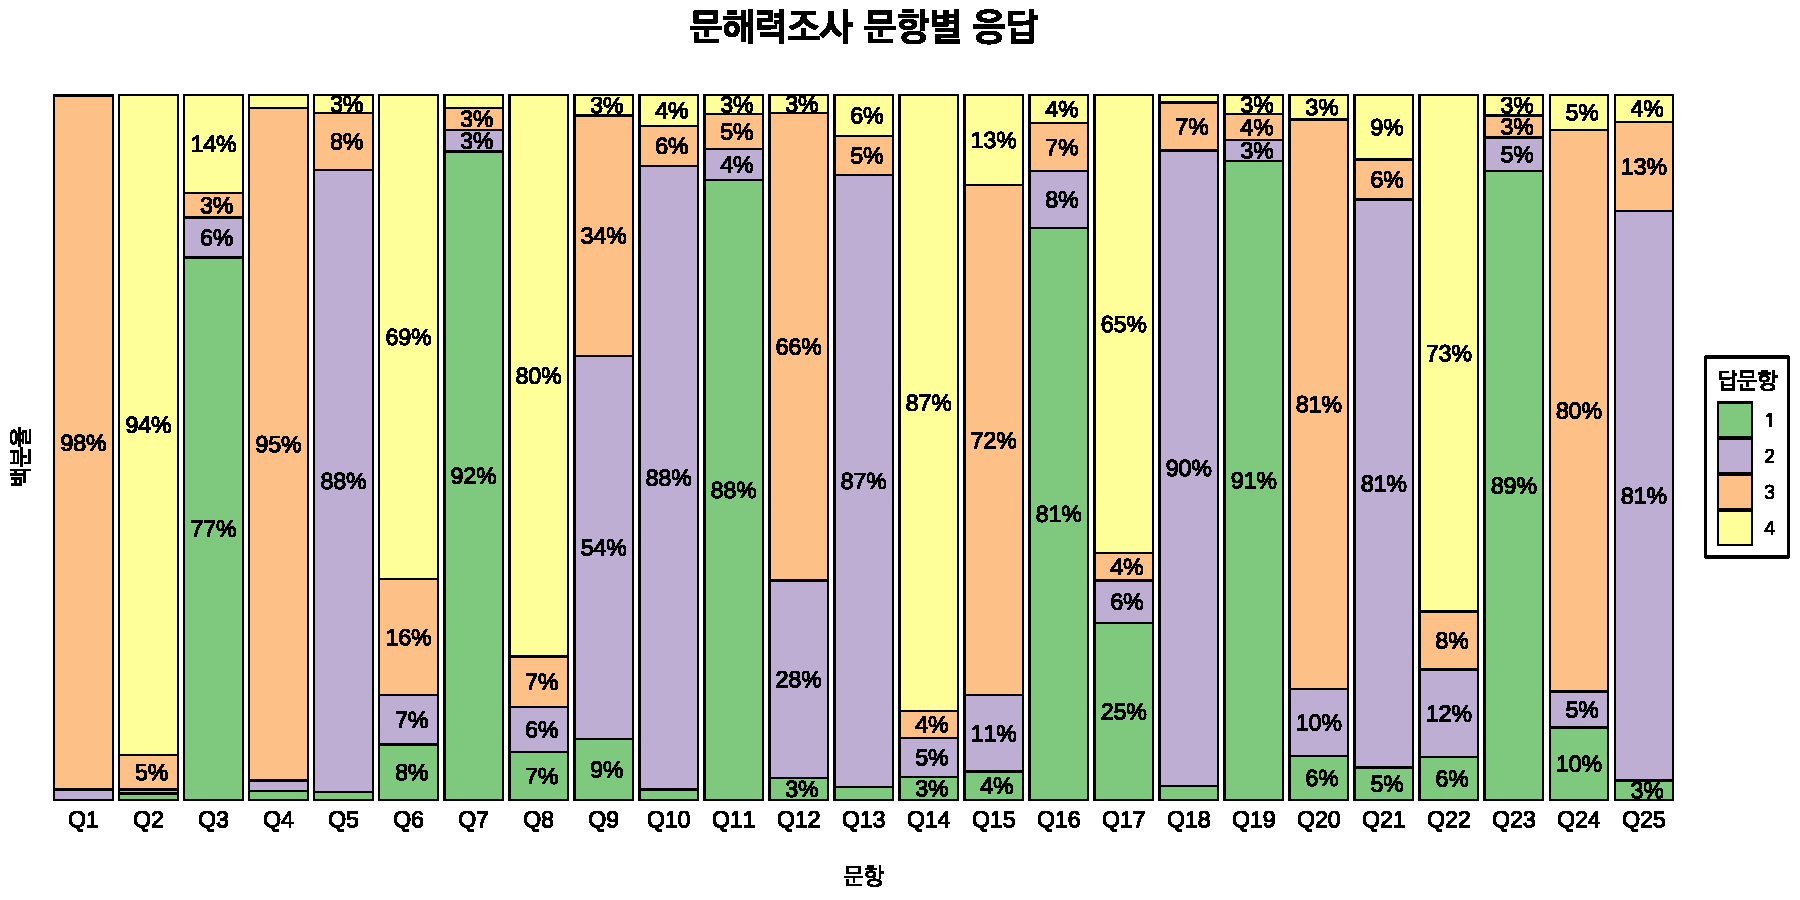
\includegraphics{_main_files/figure-latex/unnamed-chunk-5-1.pdf}

\section{문해력 점수 계산}\label{uxbb38uxd574uxb825-uxc810uxc218-uxacc4uxc0b0}

\subsection{정답과 대조하여 R(Right)/W(Wrong) 표시}\label{uxc815uxb2f5uxacfc-uxb300uxc870uxd558uxc5ec-rrightwwrong-uxd45cuxc2dc}

\begin{longtable}[]{@{}
  >{\raggedleft\arraybackslash}p{(\columnwidth - 48\tabcolsep) * \real{0.0355}}
  >{\raggedleft\arraybackslash}p{(\columnwidth - 48\tabcolsep) * \real{0.0355}}
  >{\raggedleft\arraybackslash}p{(\columnwidth - 48\tabcolsep) * \real{0.0355}}
  >{\raggedleft\arraybackslash}p{(\columnwidth - 48\tabcolsep) * \real{0.0355}}
  >{\raggedleft\arraybackslash}p{(\columnwidth - 48\tabcolsep) * \real{0.0355}}
  >{\raggedleft\arraybackslash}p{(\columnwidth - 48\tabcolsep) * \real{0.0355}}
  >{\raggedleft\arraybackslash}p{(\columnwidth - 48\tabcolsep) * \real{0.0355}}
  >{\raggedleft\arraybackslash}p{(\columnwidth - 48\tabcolsep) * \real{0.0355}}
  >{\raggedleft\arraybackslash}p{(\columnwidth - 48\tabcolsep) * \real{0.0355}}
  >{\raggedleft\arraybackslash}p{(\columnwidth - 48\tabcolsep) * \real{0.0426}}
  >{\raggedleft\arraybackslash}p{(\columnwidth - 48\tabcolsep) * \real{0.0426}}
  >{\raggedleft\arraybackslash}p{(\columnwidth - 48\tabcolsep) * \real{0.0426}}
  >{\raggedleft\arraybackslash}p{(\columnwidth - 48\tabcolsep) * \real{0.0426}}
  >{\raggedleft\arraybackslash}p{(\columnwidth - 48\tabcolsep) * \real{0.0426}}
  >{\raggedleft\arraybackslash}p{(\columnwidth - 48\tabcolsep) * \real{0.0426}}
  >{\raggedleft\arraybackslash}p{(\columnwidth - 48\tabcolsep) * \real{0.0426}}
  >{\raggedleft\arraybackslash}p{(\columnwidth - 48\tabcolsep) * \real{0.0426}}
  >{\raggedleft\arraybackslash}p{(\columnwidth - 48\tabcolsep) * \real{0.0426}}
  >{\raggedleft\arraybackslash}p{(\columnwidth - 48\tabcolsep) * \real{0.0426}}
  >{\raggedleft\arraybackslash}p{(\columnwidth - 48\tabcolsep) * \real{0.0426}}
  >{\raggedleft\arraybackslash}p{(\columnwidth - 48\tabcolsep) * \real{0.0426}}
  >{\raggedleft\arraybackslash}p{(\columnwidth - 48\tabcolsep) * \real{0.0426}}
  >{\raggedleft\arraybackslash}p{(\columnwidth - 48\tabcolsep) * \real{0.0426}}
  >{\raggedleft\arraybackslash}p{(\columnwidth - 48\tabcolsep) * \real{0.0426}}
  >{\raggedleft\arraybackslash}p{(\columnwidth - 48\tabcolsep) * \real{0.0426}}@{}}
\toprule\noalign{}
\begin{minipage}[b]{\linewidth}\raggedleft
Q1
\end{minipage} & \begin{minipage}[b]{\linewidth}\raggedleft
Q2
\end{minipage} & \begin{minipage}[b]{\linewidth}\raggedleft
Q3
\end{minipage} & \begin{minipage}[b]{\linewidth}\raggedleft
Q4
\end{minipage} & \begin{minipage}[b]{\linewidth}\raggedleft
Q5
\end{minipage} & \begin{minipage}[b]{\linewidth}\raggedleft
Q6
\end{minipage} & \begin{minipage}[b]{\linewidth}\raggedleft
Q7
\end{minipage} & \begin{minipage}[b]{\linewidth}\raggedleft
Q8
\end{minipage} & \begin{minipage}[b]{\linewidth}\raggedleft
Q9
\end{minipage} & \begin{minipage}[b]{\linewidth}\raggedleft
Q10
\end{minipage} & \begin{minipage}[b]{\linewidth}\raggedleft
Q11
\end{minipage} & \begin{minipage}[b]{\linewidth}\raggedleft
Q12
\end{minipage} & \begin{minipage}[b]{\linewidth}\raggedleft
Q13
\end{minipage} & \begin{minipage}[b]{\linewidth}\raggedleft
Q14
\end{minipage} & \begin{minipage}[b]{\linewidth}\raggedleft
Q15
\end{minipage} & \begin{minipage}[b]{\linewidth}\raggedleft
Q16
\end{minipage} & \begin{minipage}[b]{\linewidth}\raggedleft
Q17
\end{minipage} & \begin{minipage}[b]{\linewidth}\raggedleft
Q18
\end{minipage} & \begin{minipage}[b]{\linewidth}\raggedleft
Q19
\end{minipage} & \begin{minipage}[b]{\linewidth}\raggedleft
Q20
\end{minipage} & \begin{minipage}[b]{\linewidth}\raggedleft
Q21
\end{minipage} & \begin{minipage}[b]{\linewidth}\raggedleft
Q22
\end{minipage} & \begin{minipage}[b]{\linewidth}\raggedleft
Q23
\end{minipage} & \begin{minipage}[b]{\linewidth}\raggedleft
Q24
\end{minipage} & \begin{minipage}[b]{\linewidth}\raggedleft
Q25
\end{minipage} \\
\midrule\noalign{}
\endhead
\bottomrule\noalign{}
\endlastfoot
R & R & R & R & R & W & W & W & W & W & R & R & R & R & R & R & R & R & R & R & R & R & R & R & R \\
R & R & R & R & R & R & R & R & R & R & R & R & R & R & R & R & W & R & R & R & R & R & R & R & R \\
R & R & R & R & R & R & R & R & R & R & R & R & R & R & R & R & W & R & R & R & R & R & R & R & R \\
R & R & R & R & R & R & R & R & R & R & R & R & R & R & R & R & R & R & R & R & R & R & R & R & R \\
R & R & R & R & R & R & R & W & W & R & R & W & R & R & W & R & W & R & R & W & R & R & R & R & R \\
R & R & R & R & R & R & R & R & R & R & R & R & R & R & R & R & R & R & R & R & R & R & R & R & R \\
\end{longtable}

\subsection{학생별 점수 산출}\label{uxd559uxc0dduxbcc4-uxc810uxc218-uxc0b0uxcd9c}

\emph{80}, \emph{96}, \emph{96}, \emph{100}, \emph{76}, \emph{100}, \emph{88}, \emph{20}, \emph{92}, \emph{92}, \emph{88}, \emph{80}, \emph{100}, \emph{100}, \emph{80}, \emph{100}, \emph{92}, \emph{84}, \emph{100}, \emph{92}, \emph{84}, \emph{100}, \emph{92}, \emph{100}, \emph{96}, \emph{92}, \emph{84}, \emph{88}, \emph{48}, \emph{92}, \emph{96}, \emph{100}, \emph{80}, \emph{96}, \emph{92}, \emph{84}, \emph{92}, \emph{72}, \emph{96}, \emph{96}, \emph{96}, \emph{60}, \emph{100}, \emph{76}, \emph{76}, \emph{72}, \emph{80}, \emph{32}, \emph{64}, \emph{88}, \emph{92}, \emph{92}, \emph{92}, \emph{88}, \emph{96}, \emph{96}, \emph{48}, \emph{84}, \emph{72}, \emph{100}, \emph{88}, \emph{88}, \emph{88}, \emph{92}, \emph{76}, \emph{96}, \emph{96}, \emph{84}, \emph{92}, \emph{88}, \emph{96}, \emph{88}, \emph{100}, \emph{68}, \emph{80}, \emph{76}, \emph{84}, \emph{92}, \emph{92}, \emph{92}, \emph{80}, \emph{88}, \emph{84}, \emph{56}, \emph{72}, \emph{80}, \emph{84}, \emph{28}, \emph{100}, \emph{96}, \emph{92}, \emph{92}, \emph{88}, \emph{84}, \emph{88}, \emph{96}, \emph{84}, \emph{84}, \emph{88}, \emph{88}, \emph{92}, \emph{88}, \emph{88}, \emph{84}, \emph{76}, \emph{88}, \emph{88}, \emph{92}, \emph{44}, \emph{80}, \emph{84}, \emph{20}, \emph{80}, \emph{72}, \emph{92}, \emph{100}, \emph{96}, \emph{92}, \emph{88}, \emph{72}, \emph{88}, \emph{64}, \emph{56}, \emph{96}, \emph{80}, \emph{92}, \emph{84}, \emph{88}, \emph{76}, \emph{80}, \emph{84}, \emph{76}, \emph{88}, \emph{36}, \emph{80}, \emph{92}, \emph{84}, \emph{68}, \emph{80}, \emph{76}, \emph{80}, \emph{96}, \emph{96}, \emph{84}, \emph{96}, \emph{88}, \emph{68}, \emph{92}, \emph{92}, \emph{88}, \emph{92}, \emph{28}, \emph{80}, \emph{44}, \emph{100}, \emph{84}, \emph{84}, \emph{96}, \emph{68}, \emph{100}, \emph{88}, \emph{84}, \emph{92}, \emph{92}, \emph{100}, \emph{96}, \emph{92}, \emph{96}, \emph{12}, \emph{92}, \emph{72}, \emph{92}, \emph{88}, \emph{100}, \emph{20}, \emph{80}, \emph{92}, \emph{100}, \emph{100}, \emph{100}, \emph{92}, \emph{100}, \emph{92}, \emph{92}, \emph{80}, \emph{84}, \emph{92}, \emph{88}, \emph{88}, \emph{100}, \emph{88}, \emph{88}, \emph{96}, \emph{92}, \emph{80}, \emph{100}, \emph{92}, \emph{88}, \emph{96}, \emph{84}, \emph{96}, \emph{96}, \emph{96}, \emph{80}, \emph{96}, \emph{96}, \emph{52}, \emph{80}, \emph{84}, \emph{68}, \emph{92}, \emph{84}, \emph{80}, \emph{48}, \emph{84}, \emph{80}, \emph{88}, \emph{84}, \emph{96}, \emph{36}, \emph{88}, \emph{92}, \emph{88}, \emph{88}, \emph{60}, \emph{80}, \emph{84}, \emph{88}, \emph{92}, \emph{84}, \emph{64}, \emph{92}, \emph{92}, \emph{96}, \emph{88}, \emph{88}, \emph{88}, \emph{88}, \emph{88}, \emph{36}, \emph{64}, \emph{84}, \emph{76}, \emph{80}, \emph{80}, \emph{24}, \emph{100}, \emph{88}, \emph{80}, \emph{88}, \emph{92}, \emph{64}, \emph{76}, \emph{80}, \emph{24}, \emph{80}, \emph{96}, \emph{56}, \emph{64}, \emph{84}, \emph{88}, \emph{64}, \emph{84}, \emph{84}, \emph{96}, \emph{84}, \emph{92}, \emph{88}, \emph{80}, \emph{84}, \emph{24}, \emph{76}, \emph{48}, \emph{96}, \emph{88}, \emph{40}, \emph{80}, \emph{84}, \emph{80}, \emph{88}, \emph{92}, \emph{92}, \emph{80}, \emph{96}, \emph{64}, \emph{96}, \emph{40}, \emph{92}, \emph{92}, \emph{88}, \emph{84}, \emph{100}, \emph{36}, \emph{80}, \emph{92}, \emph{84}, \emph{84}, \emph{32}, \emph{96}, \emph{96}, \emph{96}, \emph{96}, \emph{96}, \emph{92}, \emph{92}, \emph{96}, \emph{84}, \emph{88}, \emph{92}, \emph{92}, \emph{88}, \emph{84}, \emph{80}, \emph{100}, \emph{80}, \emph{64}, \emph{28}, \emph{92}, \emph{88}, \emph{80}, \emph{92}, \emph{100}, \emph{92}, \emph{88}, \emph{100}, \emph{84}, \emph{80}, \emph{56}, \emph{84}, \emph{16}, \emph{76}, \emph{96}, \emph{80}, \emph{84}, \emph{68}, \emph{92}, \emph{88}, \emph{84}, \emph{88}, \emph{96}, \emph{88}, \emph{56}, \emph{36}, \emph{88}, \emph{88}, \emph{72}, \emph{76}, \emph{92}, \emph{96}, \emph{80}, \emph{92}, \emph{100}, \emph{80}, \emph{48}, \emph{28}, \emph{36}, \emph{92}, \emph{88}, \emph{84}, \emph{68}, \emph{88}, \emph{36}, \emph{92}, \emph{88}, \emph{92}, \emph{72}, \emph{84}, \emph{96}, \emph{60}, \emph{88}, \emph{96}, \emph{84}, \emph{92}, \emph{72}, \emph{100}, \emph{84}, \emph{88}, \emph{96}, \emph{80}, \emph{96}, \emph{72}, \emph{96}, \emph{80}, \emph{24}, \emph{88}, \emph{96}, \emph{36}, \emph{64}, \emph{80}, \emph{88}, \emph{92}, \emph{92}, \emph{80}, \emph{96}, \emph{92}, \emph{88}, \emph{80}, \emph{96}, \emph{88}, \emph{80}, \emph{52}, \emph{92}, \emph{92}, \emph{44}, \emph{96}, \emph{44}, \emph{88}, \emph{100}, \emph{88}, \emph{92}, \emph{96}, \emph{100}, \emph{92}, \emph{96}, \emph{88}, \emph{92}, \emph{96}, \emph{36}, \emph{92}, \emph{84}, \emph{88}, \emph{92}, \emph{56}, \emph{84}, \emph{72}, \emph{84}, \emph{88}, \emph{96}, \emph{100}, \emph{96}, \emph{76}, \emph{76}, \emph{88}, \emph{88}, \emph{88}, \emph{96}, \emph{92}, \emph{28}, \emph{96}, \emph{92}, \emph{88}, \emph{84}, \emph{76}, \emph{100}, \emph{92}, \emph{92}, \emph{88}, \emph{100}, \emph{84}, \emph{60}, \emph{84}, \emph{84}, \emph{84}, \emph{76}, \emph{100}, \emph{100}, \emph{92}, \emph{16}, \emph{84}, \emph{52}, \emph{84}, \emph{88}, \emph{88}, \emph{96}, \emph{96}, \emph{88}, \emph{88}, \emph{80}, \emph{56}, \emph{92}, \emph{28}, \emph{76}, \emph{72}, \emph{96}, \emph{80}, \emph{84}, \emph{40}, \emph{88}, \emph{88}, \emph{80}, \emph{96}, \emph{76}, \emph{96}, \emph{100}, \emph{32}, \emph{76}, \emph{88}, \emph{100}, \emph{100}, \emph{36}, \emph{92}, \emph{16}, \emph{84}, \emph{96}, \emph{92}, \emph{88}, \emph{52}, \emph{80}, \emph{84}, \emph{92}, \emph{40}, \emph{96}, \emph{96}, \emph{32}, \emph{48}, \emph{60}, \emph{92}, \emph{96}, \emph{68}, \emph{48}, \emph{48}, \emph{88}, \emph{52}, \emph{92}, \emph{52}, \emph{88}, \emph{80}, \emph{24}, \emph{76}, \emph{100}, \emph{88}, \emph{92}, \emph{80}, \emph{92}, \emph{88}, \emph{20}, \emph{92}, \emph{84}, \emph{52}, \emph{96}, \emph{96}, \emph{88}, \emph{52}, \emph{84}, \emph{40}, \emph{88}, \emph{48}, \emph{60}, \emph{72}, \emph{48}, \emph{64}, \emph{60}, \emph{40}, \emph{92}, \emph{76} and \emph{28}

\section{Red and Black 비교}\label{red-and-black-uxbe44uxad50}

\subsection{Summary}\label{summary}

\begin{itemize}
\item
  \textbf{Red}:

  \begin{longtable}[]{@{}
    >{\raggedleft\arraybackslash}p{(\columnwidth - 10\tabcolsep) * \real{0.0972}}
    >{\raggedleft\arraybackslash}p{(\columnwidth - 10\tabcolsep) * \real{0.1389}}
    >{\raggedleft\arraybackslash}p{(\columnwidth - 10\tabcolsep) * \real{0.1250}}
    >{\raggedleft\arraybackslash}p{(\columnwidth - 10\tabcolsep) * \real{0.0972}}
    >{\raggedleft\arraybackslash}p{(\columnwidth - 10\tabcolsep) * \real{0.1389}}
    >{\raggedleft\arraybackslash}p{(\columnwidth - 10\tabcolsep) * \real{0.0972}}@{}}
  \toprule\noalign{}
  \begin{minipage}[b]{\linewidth}\raggedleft
  Min.
  \end{minipage} & \begin{minipage}[b]{\linewidth}\raggedleft
  1st Qu.
  \end{minipage} & \begin{minipage}[b]{\linewidth}\raggedleft
  Median
  \end{minipage} & \begin{minipage}[b]{\linewidth}\raggedleft
  Mean
  \end{minipage} & \begin{minipage}[b]{\linewidth}\raggedleft
  3rd Qu.
  \end{minipage} & \begin{minipage}[b]{\linewidth}\raggedleft
  Max.
  \end{minipage} \\
  \midrule\noalign{}
  \endhead
  \bottomrule\noalign{}
  \endlastfoot
  16 & 77 & 88 & 79.9 & 92 & 100 \\
  \end{longtable}
\item
  \textbf{Black}:

  \begin{longtable}[]{@{}
    >{\raggedleft\arraybackslash}p{(\columnwidth - 10\tabcolsep) * \real{0.0972}}
    >{\raggedleft\arraybackslash}p{(\columnwidth - 10\tabcolsep) * \real{0.1389}}
    >{\raggedleft\arraybackslash}p{(\columnwidth - 10\tabcolsep) * \real{0.1250}}
    >{\raggedleft\arraybackslash}p{(\columnwidth - 10\tabcolsep) * \real{0.0972}}
    >{\raggedleft\arraybackslash}p{(\columnwidth - 10\tabcolsep) * \real{0.1389}}
    >{\raggedleft\arraybackslash}p{(\columnwidth - 10\tabcolsep) * \real{0.0972}}@{}}
  \toprule\noalign{}
  \begin{minipage}[b]{\linewidth}\raggedleft
  Min.
  \end{minipage} & \begin{minipage}[b]{\linewidth}\raggedleft
  1st Qu.
  \end{minipage} & \begin{minipage}[b]{\linewidth}\raggedleft
  Median
  \end{minipage} & \begin{minipage}[b]{\linewidth}\raggedleft
  Mean
  \end{minipage} & \begin{minipage}[b]{\linewidth}\raggedleft
  3rd Qu.
  \end{minipage} & \begin{minipage}[b]{\linewidth}\raggedleft
  Max.
  \end{minipage} \\
  \midrule\noalign{}
  \endhead
  \bottomrule\noalign{}
  \endlastfoot
  12 & 80 & 88 & 82.2 & 92 & 100 \\
  \end{longtable}
\end{itemize}

\subsection{줄기-잎 그림}\label{uxc904uxae30-uxc78e-uxadf8uxb9bc}

\begin{itemize}
\tightlist
\item
  Red
\end{itemize}

\begin{verbatim}
## 
##   The decimal point is 1 digit(s) to the right of the |
## 
##    1 | 6
##    2 | 000048888
##    3 | 222666666
##    4 | 00004488888888
##    5 | 2226666
##    6 | 0000444448888
##    7 | 222266666666666
##    8 | 00000000000000000000000000000000000044444444444444444444444448888888+28
##    9 | 22222222222222222222222222222222222222666666666666666666666666666666
##   10 | 00000000000000000000
\end{verbatim}

\begin{itemize}
\tightlist
\item
  Black
\end{itemize}

\begin{verbatim}
## 
##   The decimal point is 1 digit(s) to the right of the |
## 
##    1 | 266
##    2 | 4444888
##    3 | 26666
##    4 | 004488
##    5 | 22222666
##    6 | 0004444448888
##    7 | 2222222222666666666666
##    8 | 00000000000000000444444444444444444444444444444444444444888888888888+20
##    9 | 22222222222222222222222222222222222222222222222222222666666666666666+10
##   10 | 0000000000000000000000
\end{verbatim}

\subsection{Box Plots}\label{box-plots}

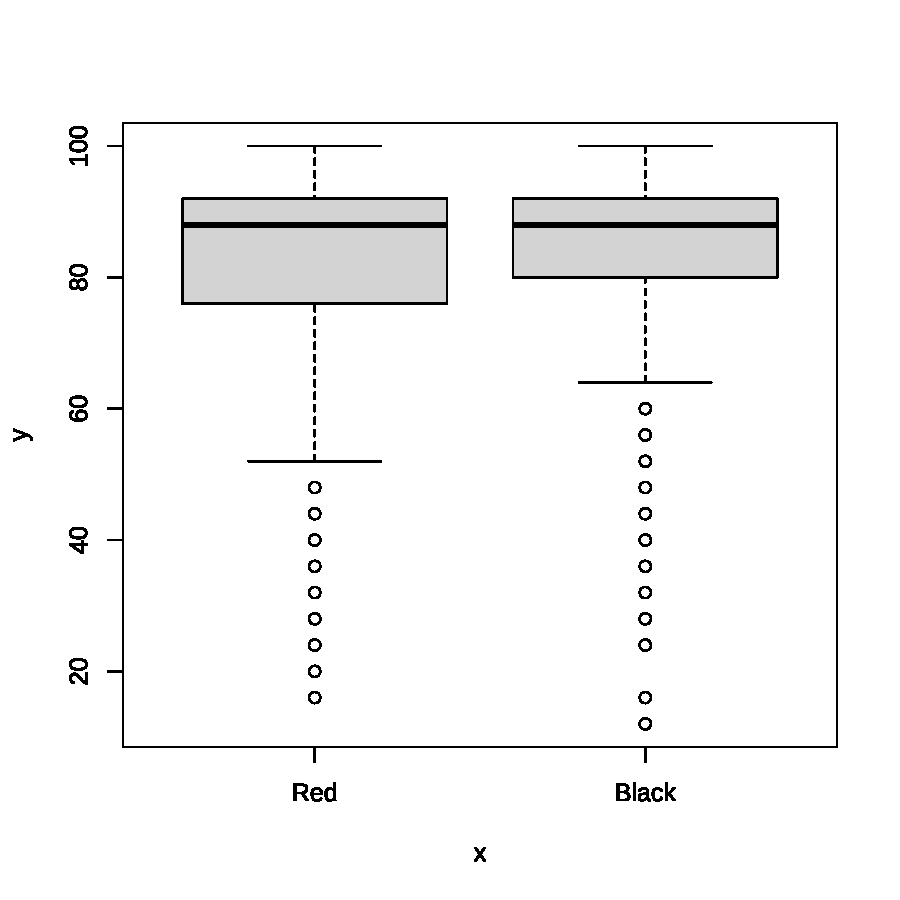
\includegraphics{_main_files/figure-latex/boxplots-1.pdf}

\subsection{QQ plot}\label{qq-plot}

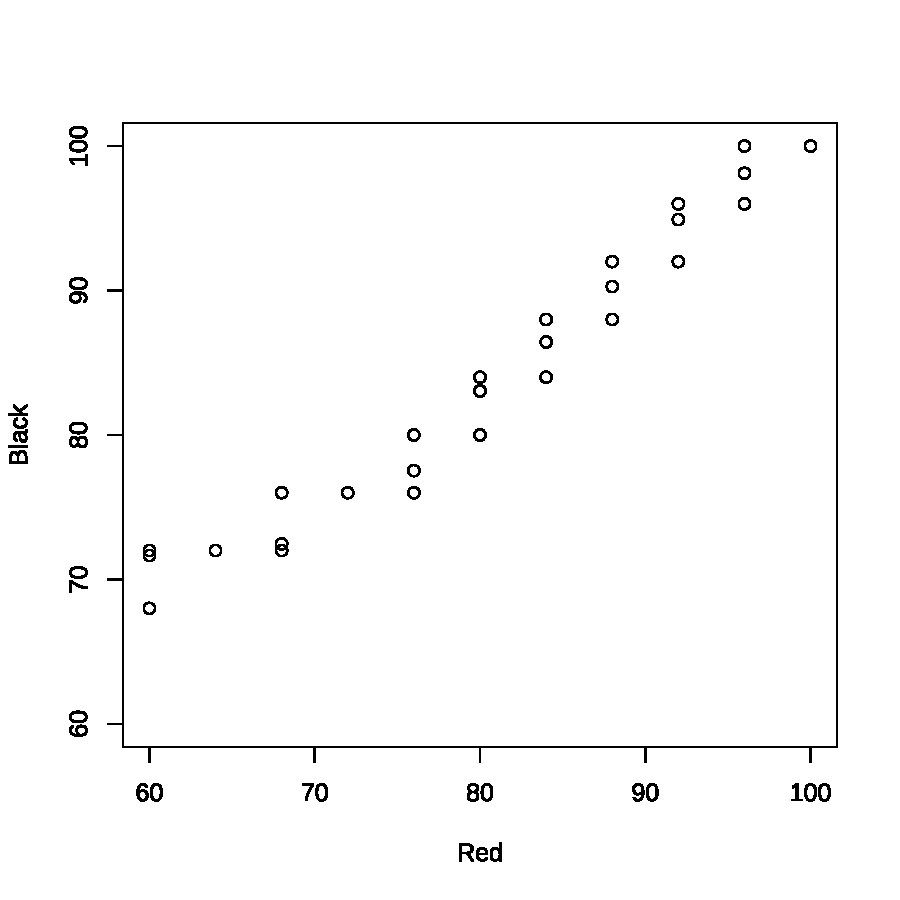
\includegraphics{_main_files/figure-latex/qqplots-1.pdf}

\subsection{ECDF plot}\label{ecdf-plot}

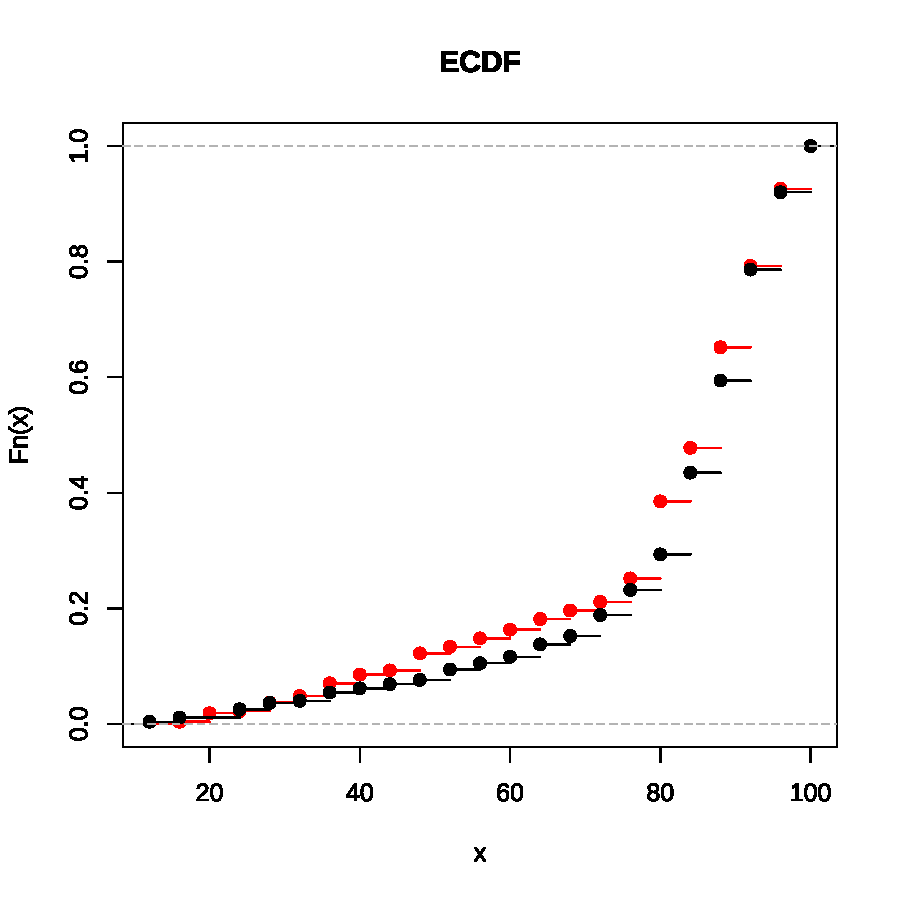
\includegraphics{_main_files/figure-latex/ECDF-1.pdf}

\subsection{t-test}\label{t-test}

Red 와 Black으로부터 관찰된 점수들의 평균에 대하여 t test를 적용하였더니 기초통계량에서 살핀 것을 뒷받침해 주듯이 p-value 가 0.05보다 큰 값이 나왔습니다. 평균은 닮았다는 뜻입니다.

\begin{longtable}[]{@{}
  >{\raggedleft\arraybackslash}p{(\columnwidth - 10\tabcolsep) * \real{0.1667}}
  >{\raggedleft\arraybackslash}p{(\columnwidth - 10\tabcolsep) * \real{0.0784}}
  >{\raggedleft\arraybackslash}p{(\columnwidth - 10\tabcolsep) * \real{0.0980}}
  >{\raggedleft\arraybackslash}p{(\columnwidth - 10\tabcolsep) * \real{0.2451}}
  >{\raggedleft\arraybackslash}p{(\columnwidth - 10\tabcolsep) * \real{0.1961}}
  >{\raggedleft\arraybackslash}p{(\columnwidth - 10\tabcolsep) * \real{0.2157}}@{}}
\caption{Welch Two Sample t-test: \texttt{score} by \texttt{.\$group}}\tabularnewline
\toprule\noalign{}
\begin{minipage}[b]{\linewidth}\raggedleft
Test statistic
\end{minipage} & \begin{minipage}[b]{\linewidth}\raggedleft
df
\end{minipage} & \begin{minipage}[b]{\linewidth}\raggedleft
P value
\end{minipage} & \begin{minipage}[b]{\linewidth}\raggedleft
Alternative hypothesis
\end{minipage} & \begin{minipage}[b]{\linewidth}\raggedleft
mean in group Red
\end{minipage} & \begin{minipage}[b]{\linewidth}\raggedleft
mean in group Black
\end{minipage} \\
\midrule\noalign{}
\endfirsthead
\toprule\noalign{}
\begin{minipage}[b]{\linewidth}\raggedleft
Test statistic
\end{minipage} & \begin{minipage}[b]{\linewidth}\raggedleft
df
\end{minipage} & \begin{minipage}[b]{\linewidth}\raggedleft
P value
\end{minipage} & \begin{minipage}[b]{\linewidth}\raggedleft
Alternative hypothesis
\end{minipage} & \begin{minipage}[b]{\linewidth}\raggedleft
mean in group Red
\end{minipage} & \begin{minipage}[b]{\linewidth}\raggedleft
mean in group Black
\end{minipage} \\
\midrule\noalign{}
\endhead
\bottomrule\noalign{}
\endlastfoot
-1.433 & 538.2 & 0.1524 & two.sided & 79.93 & 82.23 \\
\end{longtable}

\section{문해력 등급 판정}\label{uxbb38uxd574uxb825-uxb4f1uxae09-uxd310uxc815}

\subsection{분포표}\label{uxbd84uxd3ecuxd45c}

\begin{itemize}
\tightlist
\item
  I수준(24점 이하), II수준(28 \textasciitilde{} 48점), III수준(52 \textasciitilde{} 72점), IV수준(76점 이상)
\end{itemize}

\begin{table}

\caption{(\#tab:literacy grade)문해력 등급 분포}
\centering
\begin{tabular}[t]{r|r|r|r|r}
\hline
I & II & III & IV & 계\\
\hline
13 & 41 & 55 & 437 & 546\\
\hline
\end{tabular}
\end{table}

\textbackslash begin\{table\}

\textbackslash caption\{(\#tab:literacy grade)문해력 등급 분포(\%)\}
\centering

\begin{tabular}[t]{r|r|r|r|r}
\hline
I & II & III & IV & 계\\
\hline
2.38 & 7.51 & 10.07 & 80.04 & 100\\
\hline
\end{tabular}

\textbackslash end\{table\}

\subsection{Red and Black}\label{red-and-black}

\textbf{카이제곱 테스트}로 Red와 Black에 들어간 등급별 인원수가 얼마나 닮았는지를 살펴보았지만 t-test와 마찬가지로 통계적으로 유의한 차이가 관찰되지 않았습니다.

\begin{table}

\caption{(\#tab:literacy grade RnB)그룹별 문해력 등급 분포}
\centering
\begin{tabular}[t]{l|r|r|r|r|r}
\hline
  & I & II & III & IV & 계\\
\hline
Red & 6 & 27 & 24 & 213 & 270\\
\hline
Black & 7 & 14 & 31 & 224 & 276\\
\hline
계 & 13 & 41 & 55 & 437 & 546\\
\hline
\end{tabular}
\end{table}

\begin{longtable}[]{@{}
  >{\raggedleft\arraybackslash}p{(\columnwidth - 4\tabcolsep) * \real{0.2361}}
  >{\raggedleft\arraybackslash}p{(\columnwidth - 4\tabcolsep) * \real{0.0694}}
  >{\raggedleft\arraybackslash}p{(\columnwidth - 4\tabcolsep) * \real{0.1389}}@{}}
\caption{Pearson's Chi-squared test: \texttt{.}}\tabularnewline
\toprule\noalign{}
\begin{minipage}[b]{\linewidth}\raggedleft
Test statistic
\end{minipage} & \begin{minipage}[b]{\linewidth}\raggedleft
df
\end{minipage} & \begin{minipage}[b]{\linewidth}\raggedleft
P value
\end{minipage} \\
\midrule\noalign{}
\endfirsthead
\toprule\noalign{}
\begin{minipage}[b]{\linewidth}\raggedleft
Test statistic
\end{minipage} & \begin{minipage}[b]{\linewidth}\raggedleft
df
\end{minipage} & \begin{minipage}[b]{\linewidth}\raggedleft
P value
\end{minipage} \\
\midrule\noalign{}
\endhead
\bottomrule\noalign{}
\endlastfoot
5.301 & 3 & 0.151 \\
\end{longtable}

\section{유형별 정답률}\label{uxc720uxd615uxbcc4-uxc815uxb2f5uxb960}

\begin{tabular}{l|l|r}
\hline
  & 유형 & 정답률(\%)\\
\hline
문1 & 사실적 & 98.4\\
\hline
문2 & 사실적 & 93.6\\
\hline
문3 & 비판적 & 76.9\\
\hline
문4 & 사실적 & 95.4\\
\hline
문5 & 추론적 & 88.3\\
\hline
문6 & 추론적 & 68.7\\
\hline
문7 & 추론적 & 91.9\\
\hline
문8 & 사실적 & 79.7\\
\hline
문9 & 추론적 & 34.1\\
\hline
문10 & 추론적 & 88.5\\
\hline
문11 & 사실적 & 87.9\\
\hline
문12 & 사실적 & 66.3\\
\hline
문13 & 사실적 & 86.8\\
\hline
문14 & 추론적 & 87.4\\
\hline
문15 & 사실적 & 72.3\\
\hline
문16 & 사실적 & 81.1\\
\hline
문17 & 추론적 & 65.0\\
\hline
문18 & 비판적 & 90.1\\
\hline
문19 & 사실적 & 90.7\\
\hline
문20 & 사실적 & 80.8\\
\hline
문21 & 사실적 & 80.6\\
\hline
문22 & 비판적 & 73.3\\
\hline
문23 & 추론적 & 89.2\\
\hline
문24 & 사실적 & 79.7\\
\hline
문25 & 추론적 & 80.8\\
\hline
\end{tabular}

\section{어려운 문제?}\label{uxc5b4uxb824uxc6b4-uxbb38uxc81c}

\subsection{정답률 80\% 이하}\label{uxc815uxb2f5uxb960-80-uxc774uxd558}

\begin{tabular}{l|r|r|r|r|r|r|r|r|r}
\hline
  & 문3 & 문6 & 문8 & 문9 & 문12 & 문15 & 문17 & 문22 & 문24\\
\hline
정답률 & 76.9 & 68.7 & 79.7 & 34.1 & 66.3 & 72.3 & 65 & 73.3 & 79.7\\
\hline
\end{tabular}

\subsection{정답률 70\% 이하}\label{uxc815uxb2f5uxb960-70-uxc774uxd558}

\begin{tabular}{l|r|r|r|r}
\hline
  & 문6 & 문9 & 문12 & 문17\\
\hline
정답률 & 68.7 & 34.1 & 66.3 & 65\\
\hline
\end{tabular}

\subsection{정답률 60\% 이하}\label{uxc815uxb2f5uxb960-60-uxc774uxd558}

\begin{tabular}{l|r}
\hline
  & 문9\\
\hline
정답률 & 34.1\\
\hline
\end{tabular}

\subsection{정답률 50\% 이하}\label{uxc815uxb2f5uxb960-50-uxc774uxd558}

\begin{tabular}{l|r}
\hline
  & 문9\\
\hline
정답률 & 34.1\\
\hline
\end{tabular}

\section{정답률이 낮은 문제들}\label{uxc815uxb2f5uxb960uxc774-uxb0aeuxc740-uxbb38uxc81cuxb4e4}

\subsection{문6.}\label{uxbb386.}

\begin{flushleft}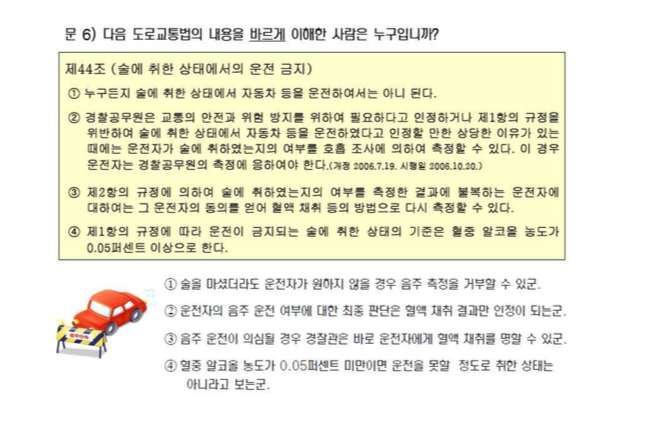
\includegraphics[width=0.75\linewidth]{./pics/Q06} \end{flushleft}

\subsection{문9.}\label{uxbb389.}

\begin{flushleft}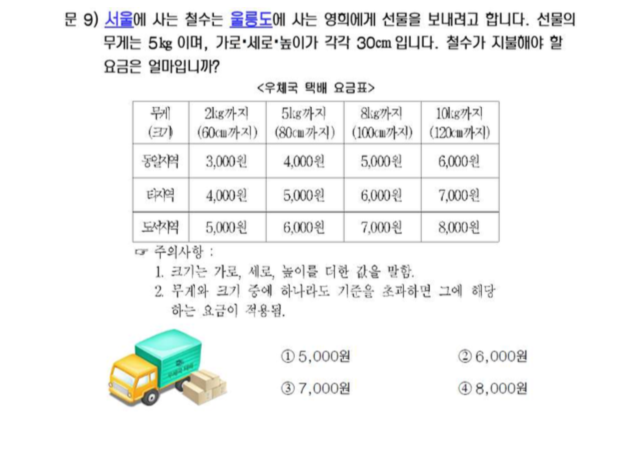
\includegraphics[width=0.75\linewidth]{./pics/Q09} \end{flushleft}

\subsection{문12.}\label{uxbb3812.}

\begin{flushleft}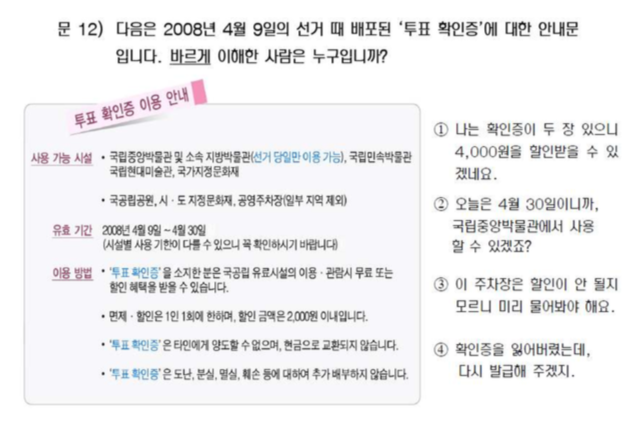
\includegraphics[width=0.75\linewidth]{./pics/Q12} \end{flushleft}

\subsection{문15.}\label{uxbb3815.}

\begin{flushleft}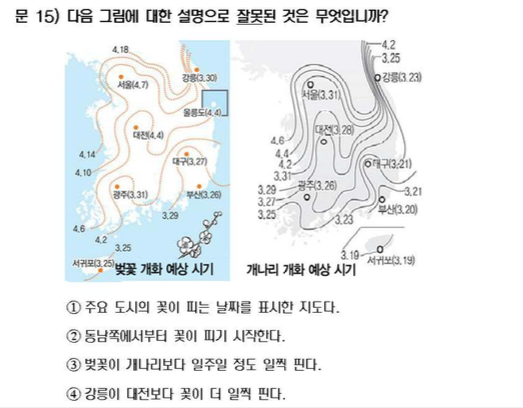
\includegraphics[width=0.75\linewidth]{./pics/Q15} \end{flushleft}

\subsection{문17.}\label{uxbb3817.}

\begin{flushleft}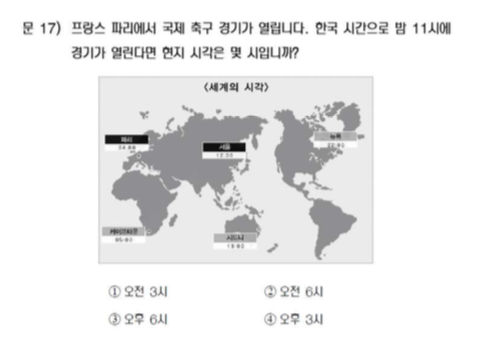
\includegraphics[width=0.75\linewidth]{./pics/Q17} \end{flushleft}

\subsection{문22.}\label{uxbb3822.}

\begin{flushleft}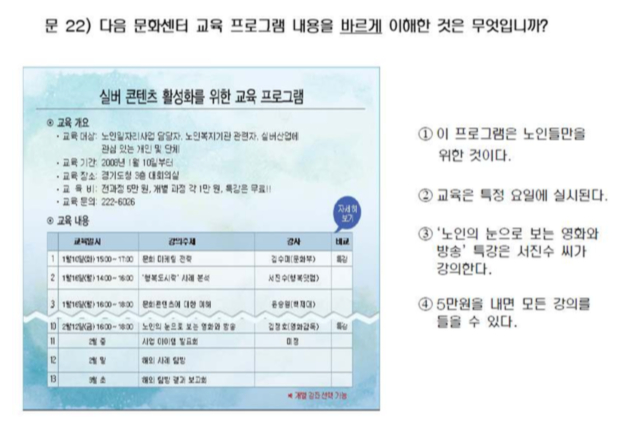
\includegraphics[width=0.75\linewidth]{./pics/Q22} \end{flushleft}

\chapter{1주차 데이터 실험 집계}\label{uxc8fcuxcc28-uxb370uxc774uxd130-uxc2e4uxd5d8-uxc9d1uxacc4}

\section{실험의 목적}\label{uxc2e4uxd5d8uxc758-uxbaa9uxc801}

1주차 구글 예습 설문지 집계결과를 분석합니다.

Q1\textasciitilde Q3에서는 랜덤화의 효과로 Red, Black 이 얼마나 닮았는지 알아봅니다.

Q4에서는 같은 내용의 질문지인데 ``바람직한 논의이다''라는 선택지에 부연설명을 붙이거나(Red), ``부적절한 논의이다''라는 선택지에 부연설명을 붙였을 때(Black), 부연설명의 여부에 따라 응답이 달라지는 지 살펴봅니다.

끝으로 제출시간의 분포가 날마다 고른지, Red, Black 간에는 닮았는지 알아봅니다.

\subsection{Red, Black을 잘못 표시한 사람들}\label{red-blackuxc744-uxc798uxbabb-uxd45cuxc2dcuxd55c-uxc0acuxb78cuxb4e4}

랜덤화출석부(2월 25일 기준)에 있는 Red, Black 과 실제 구글예습설문지에 올린 Red, Black 이 다른 사람들의 분포를 파악해 보았습니다.

\begin{longtable}[]{@{}
  >{\raggedright\arraybackslash}p{(\columnwidth - 4\tabcolsep) * \real{0.3611}}
  >{\centering\arraybackslash}p{(\columnwidth - 4\tabcolsep) * \real{0.2778}}
  >{\centering\arraybackslash}p{(\columnwidth - 4\tabcolsep) * \real{0.3056}}@{}}
\toprule\noalign{}
\begin{minipage}[b]{\linewidth}\raggedright
~
\end{minipage} & \begin{minipage}[b]{\linewidth}\centering
Red(구글예습퀴즈)
\end{minipage} & \begin{minipage}[b]{\linewidth}\centering
Black(구글예습퀴즈)
\end{minipage} \\
\midrule\noalign{}
\endhead
\bottomrule\noalign{}
\endlastfoot
\textbf{Red(랜덤화출석부)} & 286 & 8 \\
\textbf{Black(랜덤화출석부)} & 6 & 276 \\
\textbf{계} & 292 & 284 \\
\end{longtable}

랜덤화출석부에 있는 Red, Black 과 실제 구글 설문지에서 선택한 Red, Black 이 다른 사람들의 수효는 14명입니다.

Red를 Black 이라고 한 사람이 8명, Black 을 Red 라고 한 사람이 6명입니다.

두 가지 방법으로 분석합니다.

우선 Red, Black 을 잘못 선택한 14명을 랜덤하게 둘로 나누면 어느 한 쪽 집단에 들어갈 기대인원은 14명을 둘로 나눈 7(명)이고, 표준오차는 14의 제곱근에 1/2을 곱해 준 1.9명이 됩니다.

실제로 Red를 Black 이라고 한 사람수, 8명이나 Black 을 Red 라고 한 사람수, 6명은 기대인원으로부터 표준오차 범위 안에 아주 잘 들어갑니다.

두 번째 분석 방법은 확률을 계산해 보는 것입니다.

Red, Black 을 잘못 선택한 14명을 랜덤하게 둘로 나눌 때, 실제로 관찰된 8명 이상이나 6명이하로 잘못 선택한 사람수가 나올 가능성은 얼마나 되는가 입니다.

이 경우 공평한 동전던지기를 확률 법칙으로 표현한 이항분포로부터 계산할 수 있습니다.

시행횟수가 14이고 한 번 시행에서 성공확률이 1/2 인 이항분포에서 성공갯수가 6이하이거나 8이상을 관찰할 확률은 0.791입니다.

공평한 동전 던지기에서 앞면이 6개 이하 나오는 확률은 8개 이상 나오는 확률과 같기 때문에 사실상 한쪽만 계산해서 2배 해 주면 됩니다.

이 값을 p-value 라고 하는데, p-value가 0.05보다 작을 때 \textbf{통계적으로 유의한 차이를 관찰}하였다고 말합니다.

즉, 공평한 동전을 던지는 것과 같은 과정이라고 가정하였을 때 실제로 관찰된 값들이 가정으로부터 얼마나 떨어져 있는지를 표현한 것입니다.

0.05, 즉 1/20은 이런 실험을 스무 번 정도 반복하면 1번 나올 정도로 드문 사건을 의미합니다.

즉 가정이 타당하다면 나오기 힘든 결과라는 것입니다.

그런데 Red, Black 을 잘못 표시한 사람들의 분포에서 관찰된 p-value 는 0.05와는 비교도 안될 정도로 큰 값입니다.

따라서 두 집단이 랜덤화 효과가 작동하여 \textbf{통계적으로 유의한 차이를 보이지 않는다}고 할 수 있습니다.

\subsection{응답인원의 Red, Black}\label{uxc751uxb2f5uxc778uxc6d0uxc758-red-black}

Red 로 응답한 인원은 292명, Black 에 응답한 인원은 284명입니다.

전체 응답인원 576 명을 랜덤하게 둘로 나눌 때 어느 한 쪽의 기대인원은 전체 응답인원의 절반인 288명이고, 표준오차는 전체 응답인원의 제곱근에 1/2을 곱해 준 12 명입니다.

따라서 Red, Black 각 그룹에 관찰된 인원은 기대인원으로부터 표준오차 범위 안에 들어갑니다.

간혹 이 범위를 살짝 벗어나는 경우들이 가끔 나오지만 두배의 표준오차 범위 안에는 거의 다 들어갑니다.

\section{Q1. Dewey as good as elected, statistics convince Roper}\label{q1.-dewey-as-good-as-elected-statistics-convince-roper}

\begin{flushleft}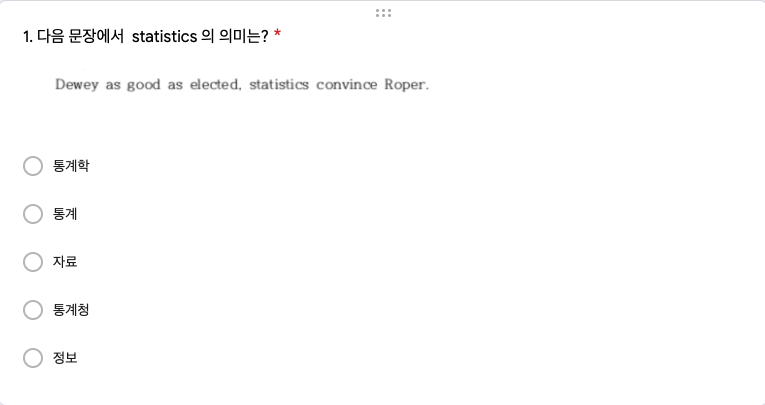
\includegraphics[width=1\linewidth]{./pics/Quiz210302_01} \end{flushleft}

\subsection{Roper(Counts)}\label{ropercounts}

\begin{longtable}[]{@{}
  >{\raggedright\arraybackslash}p{(\columnwidth - 12\tabcolsep) * \real{0.1667}}
  >{\centering\arraybackslash}p{(\columnwidth - 12\tabcolsep) * \real{0.1250}}
  >{\centering\arraybackslash}p{(\columnwidth - 12\tabcolsep) * \real{0.0972}}
  >{\centering\arraybackslash}p{(\columnwidth - 12\tabcolsep) * \real{0.0972}}
  >{\centering\arraybackslash}p{(\columnwidth - 12\tabcolsep) * \real{0.1250}}
  >{\centering\arraybackslash}p{(\columnwidth - 12\tabcolsep) * \real{0.0972}}
  >{\centering\arraybackslash}p{(\columnwidth - 12\tabcolsep) * \real{0.0972}}@{}}
\toprule\noalign{}
\begin{minipage}[b]{\linewidth}\raggedright
~
\end{minipage} & \begin{minipage}[b]{\linewidth}\centering
통계학
\end{minipage} & \begin{minipage}[b]{\linewidth}\centering
통계
\end{minipage} & \begin{minipage}[b]{\linewidth}\centering
자료
\end{minipage} & \begin{minipage}[b]{\linewidth}\centering
통계청
\end{minipage} & \begin{minipage}[b]{\linewidth}\centering
정보
\end{minipage} & \begin{minipage}[b]{\linewidth}\centering
계
\end{minipage} \\
\midrule\noalign{}
\endhead
\bottomrule\noalign{}
\endlastfoot
\textbf{Red} & 26 & 230 & 25 & 6 & 5 & 292 \\
\textbf{Black} & 13 & 244 & 14 & 8 & 5 & 284 \\
\textbf{계} & 39 & 474 & 39 & 14 & 10 & 576 \\
\end{longtable}

\begin{longtable}[]{@{}
  >{\raggedleft\arraybackslash}p{(\columnwidth - 4\tabcolsep) * \real{0.2361}}
  >{\raggedleft\arraybackslash}p{(\columnwidth - 4\tabcolsep) * \real{0.0694}}
  >{\raggedleft\arraybackslash}p{(\columnwidth - 4\tabcolsep) * \real{0.1389}}@{}}
\caption{Pearson's Chi-squared test: \texttt{.}}\tabularnewline
\toprule\noalign{}
\begin{minipage}[b]{\linewidth}\raggedleft
Test statistic
\end{minipage} & \begin{minipage}[b]{\linewidth}\raggedleft
df
\end{minipage} & \begin{minipage}[b]{\linewidth}\raggedleft
P value
\end{minipage} \\
\midrule\noalign{}
\endfirsthead
\toprule\noalign{}
\begin{minipage}[b]{\linewidth}\raggedleft
Test statistic
\end{minipage} & \begin{minipage}[b]{\linewidth}\raggedleft
df
\end{minipage} & \begin{minipage}[b]{\linewidth}\raggedleft
P value
\end{minipage} \\
\midrule\noalign{}
\endhead
\bottomrule\noalign{}
\endlastfoot
8.026 & 4 & 0.09065 \\
\end{longtable}

Q1의 집계 결과가 Red, Black 간에 통계적으로 유의한 차이가 있는지 알아보기 위하여 카이제곱 테스트를 수행하였습니다.

그 결과 카이제곱 통계량은 8.03, 자유도는 4, p-value 는 0.0906이므로 Red, Black 간에 통계적으로 유의한 차이를 보이지 않습니다.

실제로 닮은 게 느껴집니까?

\subsection{Roper(\%)}\label{roper}

\begin{longtable}[]{@{}
  >{\centering\arraybackslash}p{(\columnwidth - 10\tabcolsep) * \real{0.1250}}
  >{\centering\arraybackslash}p{(\columnwidth - 10\tabcolsep) * \real{0.0972}}
  >{\centering\arraybackslash}p{(\columnwidth - 10\tabcolsep) * \real{0.0972}}
  >{\centering\arraybackslash}p{(\columnwidth - 10\tabcolsep) * \real{0.1250}}
  >{\centering\arraybackslash}p{(\columnwidth - 10\tabcolsep) * \real{0.0972}}
  >{\centering\arraybackslash}p{(\columnwidth - 10\tabcolsep) * \real{0.1111}}@{}}
\toprule\noalign{}
\begin{minipage}[b]{\linewidth}\centering
통계학
\end{minipage} & \begin{minipage}[b]{\linewidth}\centering
통계
\end{minipage} & \begin{minipage}[b]{\linewidth}\centering
자료
\end{minipage} & \begin{minipage}[b]{\linewidth}\centering
통계청
\end{minipage} & \begin{minipage}[b]{\linewidth}\centering
정보
\end{minipage} & \begin{minipage}[b]{\linewidth}\centering
계
\end{minipage} \\
\midrule\noalign{}
\endhead
\bottomrule\noalign{}
\endlastfoot
6.8 & 82.3 & 6.8 & 2.4 & 1.7 & 100.0 \\
\end{longtable}

정답률은 Red, Black 을 합하여 계산하는데, 82.3(\%) 입니다.

\section{Q2. Statistics is the science of learning from data, \ldots{}}\label{q2.-statistics-is-the-science-of-learning-from-data}

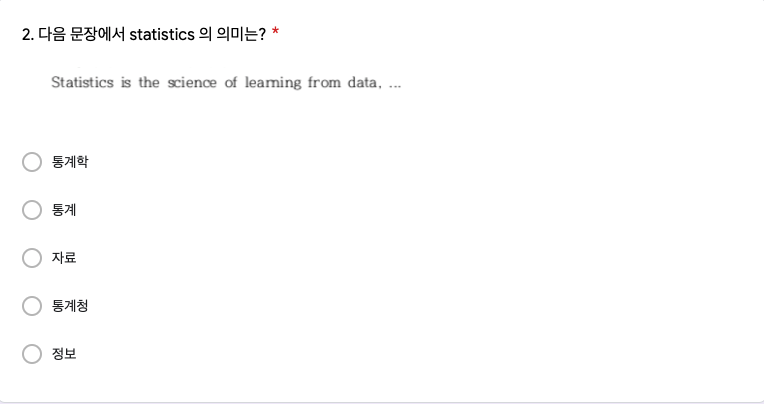
\includegraphics[width=1\linewidth]{./pics/Quiz210302_02}

\subsection{ASA(Counts)}\label{asacounts}

\begin{longtable}[]{@{}
  >{\raggedright\arraybackslash}p{(\columnwidth - 12\tabcolsep) * \real{0.1667}}
  >{\centering\arraybackslash}p{(\columnwidth - 12\tabcolsep) * \real{0.1250}}
  >{\centering\arraybackslash}p{(\columnwidth - 12\tabcolsep) * \real{0.0972}}
  >{\centering\arraybackslash}p{(\columnwidth - 12\tabcolsep) * \real{0.0972}}
  >{\centering\arraybackslash}p{(\columnwidth - 12\tabcolsep) * \real{0.1250}}
  >{\centering\arraybackslash}p{(\columnwidth - 12\tabcolsep) * \real{0.0972}}
  >{\centering\arraybackslash}p{(\columnwidth - 12\tabcolsep) * \real{0.0972}}@{}}
\toprule\noalign{}
\begin{minipage}[b]{\linewidth}\raggedright
~
\end{minipage} & \begin{minipage}[b]{\linewidth}\centering
통계학
\end{minipage} & \begin{minipage}[b]{\linewidth}\centering
통계
\end{minipage} & \begin{minipage}[b]{\linewidth}\centering
자료
\end{minipage} & \begin{minipage}[b]{\linewidth}\centering
통계청
\end{minipage} & \begin{minipage}[b]{\linewidth}\centering
정보
\end{minipage} & \begin{minipage}[b]{\linewidth}\centering
계
\end{minipage} \\
\midrule\noalign{}
\endhead
\bottomrule\noalign{}
\endlastfoot
\textbf{Red} & 257 & 27 & 4 & 3 & 1 & 292 \\
\textbf{Black} & 262 & 14 & 3 & 2 & 3 & 284 \\
\textbf{계} & 519 & 41 & 7 & 5 & 4 & 576 \\
\end{longtable}

\begin{longtable}[]{@{}
  >{\raggedleft\arraybackslash}p{(\columnwidth - 4\tabcolsep) * \real{0.2361}}
  >{\raggedleft\arraybackslash}p{(\columnwidth - 4\tabcolsep) * \real{0.0694}}
  >{\raggedleft\arraybackslash}p{(\columnwidth - 4\tabcolsep) * \real{0.1389}}@{}}
\caption{Pearson's Chi-squared test: \texttt{.}}\tabularnewline
\toprule\noalign{}
\begin{minipage}[b]{\linewidth}\raggedleft
Test statistic
\end{minipage} & \begin{minipage}[b]{\linewidth}\raggedleft
df
\end{minipage} & \begin{minipage}[b]{\linewidth}\raggedleft
P value
\end{minipage} \\
\midrule\noalign{}
\endfirsthead
\toprule\noalign{}
\begin{minipage}[b]{\linewidth}\raggedleft
Test statistic
\end{minipage} & \begin{minipage}[b]{\linewidth}\raggedleft
df
\end{minipage} & \begin{minipage}[b]{\linewidth}\raggedleft
P value
\end{minipage} \\
\midrule\noalign{}
\endhead
\bottomrule\noalign{}
\endlastfoot
5.403 & 4 & 0.2484 \\
\end{longtable}

Q2의 집계 결과가 Red, Black 간에 통계적으로 유의한 차이가 있는지 알아보기 위하여 카이제곱 테스트를 수행하였습니다.

그 결과 카이제곱 통계량은 5.403, 자유도는 4, p-value 는 0.2484이므로 Red, Black 간에 통계적으로 유의한 차이를 보이지 않습니다.

실제로 닮은 게 느껴집니까?

\subsection{ASA(\%)}\label{asa}

\begin{longtable}[]{@{}
  >{\centering\arraybackslash}p{(\columnwidth - 10\tabcolsep) * \real{0.1250}}
  >{\centering\arraybackslash}p{(\columnwidth - 10\tabcolsep) * \real{0.0972}}
  >{\centering\arraybackslash}p{(\columnwidth - 10\tabcolsep) * \real{0.0972}}
  >{\centering\arraybackslash}p{(\columnwidth - 10\tabcolsep) * \real{0.1250}}
  >{\centering\arraybackslash}p{(\columnwidth - 10\tabcolsep) * \real{0.0972}}
  >{\centering\arraybackslash}p{(\columnwidth - 10\tabcolsep) * \real{0.1250}}@{}}
\toprule\noalign{}
\begin{minipage}[b]{\linewidth}\centering
통계학
\end{minipage} & \begin{minipage}[b]{\linewidth}\centering
통계
\end{minipage} & \begin{minipage}[b]{\linewidth}\centering
자료
\end{minipage} & \begin{minipage}[b]{\linewidth}\centering
통계청
\end{minipage} & \begin{minipage}[b]{\linewidth}\centering
정보
\end{minipage} & \begin{minipage}[b]{\linewidth}\centering
계
\end{minipage} \\
\midrule\noalign{}
\endhead
\bottomrule\noalign{}
\endlastfoot
90.10 & 7.12 & 1.22 & 0.87 & 0.69 & 100.00 \\
\end{longtable}

정답률은 Red, Black 을 합하여 계산하는데, 90.1(\%) 입니다.

\section{Q3. How to lie with statistics}\label{q3.-how-to-lie-with-statistics}

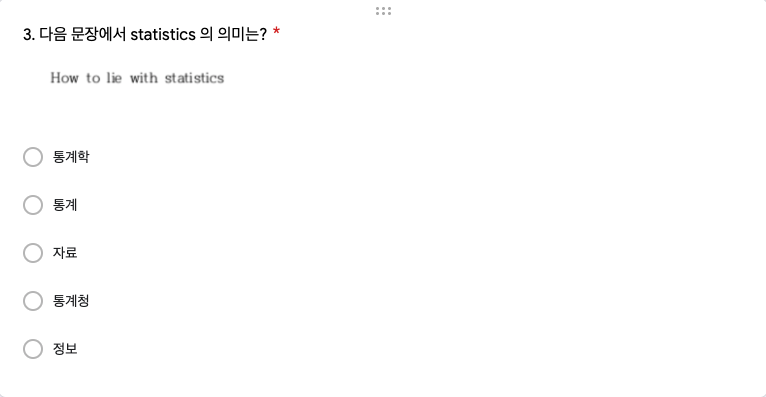
\includegraphics[width=1\linewidth]{./pics/Quiz210302_03}

\subsection{D.Huff(Counts)}\label{d.huffcounts}

\begin{longtable}[]{@{}
  >{\raggedright\arraybackslash}p{(\columnwidth - 12\tabcolsep) * \real{0.1667}}
  >{\centering\arraybackslash}p{(\columnwidth - 12\tabcolsep) * \real{0.1250}}
  >{\centering\arraybackslash}p{(\columnwidth - 12\tabcolsep) * \real{0.0972}}
  >{\centering\arraybackslash}p{(\columnwidth - 12\tabcolsep) * \real{0.0972}}
  >{\centering\arraybackslash}p{(\columnwidth - 12\tabcolsep) * \real{0.1250}}
  >{\centering\arraybackslash}p{(\columnwidth - 12\tabcolsep) * \real{0.0972}}
  >{\centering\arraybackslash}p{(\columnwidth - 12\tabcolsep) * \real{0.0972}}@{}}
\toprule\noalign{}
\begin{minipage}[b]{\linewidth}\raggedright
~
\end{minipage} & \begin{minipage}[b]{\linewidth}\centering
통계학
\end{minipage} & \begin{minipage}[b]{\linewidth}\centering
통계
\end{minipage} & \begin{minipage}[b]{\linewidth}\centering
자료
\end{minipage} & \begin{minipage}[b]{\linewidth}\centering
통계청
\end{minipage} & \begin{minipage}[b]{\linewidth}\centering
정보
\end{minipage} & \begin{minipage}[b]{\linewidth}\centering
계
\end{minipage} \\
\midrule\noalign{}
\endhead
\bottomrule\noalign{}
\endlastfoot
\textbf{Red} & 14 & 204 & 41 & 14 & 19 & 292 \\
\textbf{Black} & 16 & 213 & 28 & 6 & 21 & 284 \\
\textbf{계} & 30 & 417 & 69 & 20 & 40 & 576 \\
\end{longtable}

\begin{longtable}[]{@{}
  >{\raggedleft\arraybackslash}p{(\columnwidth - 4\tabcolsep) * \real{0.2361}}
  >{\raggedleft\arraybackslash}p{(\columnwidth - 4\tabcolsep) * \real{0.0694}}
  >{\raggedleft\arraybackslash}p{(\columnwidth - 4\tabcolsep) * \real{0.1389}}@{}}
\caption{Pearson's Chi-squared test: \texttt{.}}\tabularnewline
\toprule\noalign{}
\begin{minipage}[b]{\linewidth}\raggedleft
Test statistic
\end{minipage} & \begin{minipage}[b]{\linewidth}\raggedleft
df
\end{minipage} & \begin{minipage}[b]{\linewidth}\raggedleft
P value
\end{minipage} \\
\midrule\noalign{}
\endfirsthead
\toprule\noalign{}
\begin{minipage}[b]{\linewidth}\raggedleft
Test statistic
\end{minipage} & \begin{minipage}[b]{\linewidth}\raggedleft
df
\end{minipage} & \begin{minipage}[b]{\linewidth}\raggedleft
P value
\end{minipage} \\
\midrule\noalign{}
\endhead
\bottomrule\noalign{}
\endlastfoot
5.967 & 4 & 0.2016 \\
\end{longtable}

Q3의 집계 결과가 Red, Black 간에 통계적으로 유의한 차이가 있는지 알아보기 위하여 카이제곱 테스트를 수행하였습니다.

그 결과 카이제곱 통계량은 5.967, 자유도는 4, p-value 는 0.2016이므로 Red, Black 간에 통계적으로 유의한 차이를 보이지 않습니다.

실제로 닮은 게 느껴집니까?

\subsection{D.Huff(\%)}\label{d.huff}

\begin{longtable}[]{@{}
  >{\centering\arraybackslash}p{(\columnwidth - 10\tabcolsep) * \real{0.1250}}
  >{\centering\arraybackslash}p{(\columnwidth - 10\tabcolsep) * \real{0.0972}}
  >{\centering\arraybackslash}p{(\columnwidth - 10\tabcolsep) * \real{0.0972}}
  >{\centering\arraybackslash}p{(\columnwidth - 10\tabcolsep) * \real{0.1250}}
  >{\centering\arraybackslash}p{(\columnwidth - 10\tabcolsep) * \real{0.0972}}
  >{\centering\arraybackslash}p{(\columnwidth - 10\tabcolsep) * \real{0.1111}}@{}}
\toprule\noalign{}
\begin{minipage}[b]{\linewidth}\centering
통계학
\end{minipage} & \begin{minipage}[b]{\linewidth}\centering
통계
\end{minipage} & \begin{minipage}[b]{\linewidth}\centering
자료
\end{minipage} & \begin{minipage}[b]{\linewidth}\centering
통계청
\end{minipage} & \begin{minipage}[b]{\linewidth}\centering
정보
\end{minipage} & \begin{minipage}[b]{\linewidth}\centering
계
\end{minipage} \\
\midrule\noalign{}
\endhead
\bottomrule\noalign{}
\endlastfoot
5.2 & 72.4 & 12.0 & 3.5 & 6.9 & 100.0 \\
\end{longtable}

정답률은 Red, Black 을 합하여 계산하는데, 72.4(\%) 입니다.

\section{Q4. 종부세}\label{q4.-uxc885uxbd80uxc138}

``바람직한 논의이다''라는 선택지에 부연설명을 붙이거나(Red), ``부적절한 논의이다''라는 선택지에 부연설명을 붙였을 때(Black), 부연설명의 여부에 따라 응답이 달라지는 지 살펴본 결과 기대와는 달리 통계적으로 유의한 수준의 차이를 관찰하지 못하였습니다.

앞에서 본 바와 같이 Red, Black 두 집단은 출석부의 다섯 변수에 대하여 랜덤화 과정을 거쳐서 가장 닮은 구성을 찾은 것이기에 Q1, Q2, Q3의 응답 결과도 매우 닮게 나오는데 만약 부연설명이 효과가 없다면 Q4에서의 응답도 닮게 나왔을 것입니다.

지난 학기들과 달리 통계적으로 유의한 차이를 관찰하지 못한 이유를 따져 볼 필요가 있겠습니다.

\subsection{질문지 선택지에 부연설명}\label{uxc9c8uxbb38uxc9c0-uxc120uxd0dduxc9c0uxc5d0-uxbd80uxc5f0uxc124uxba85}

\begin{flushleft}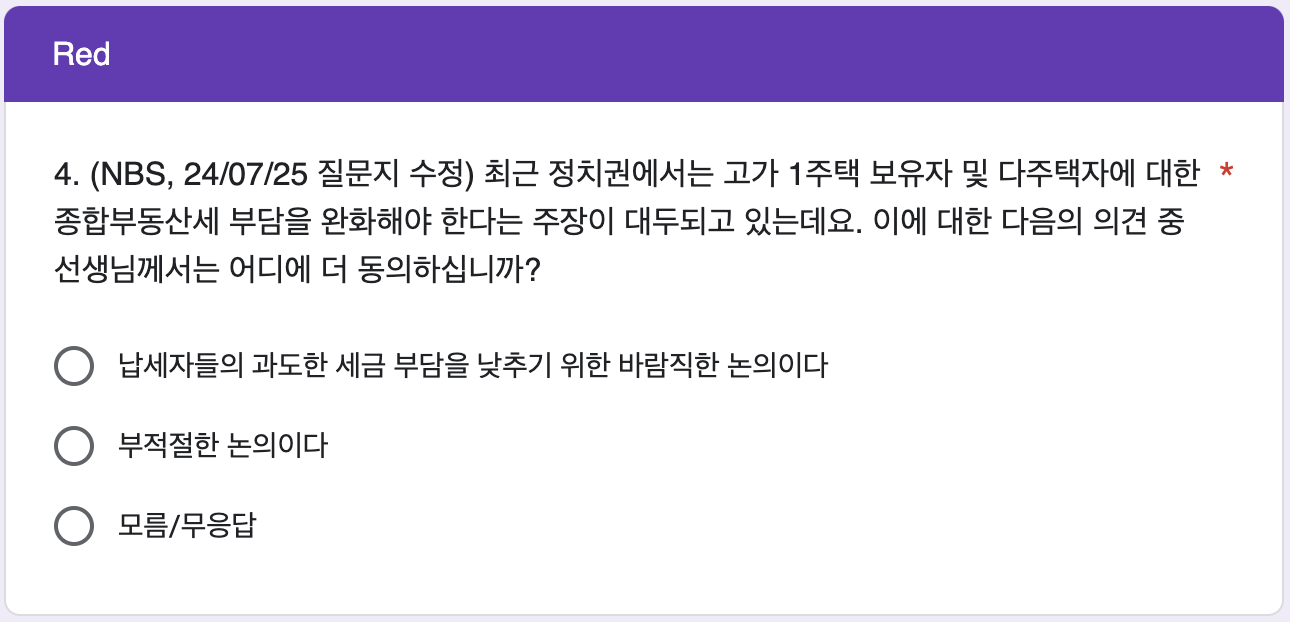
\includegraphics[width=0.67\linewidth]{./pics/Quiz240902_Q4_Red} \end{flushleft}

\begin{flushleft}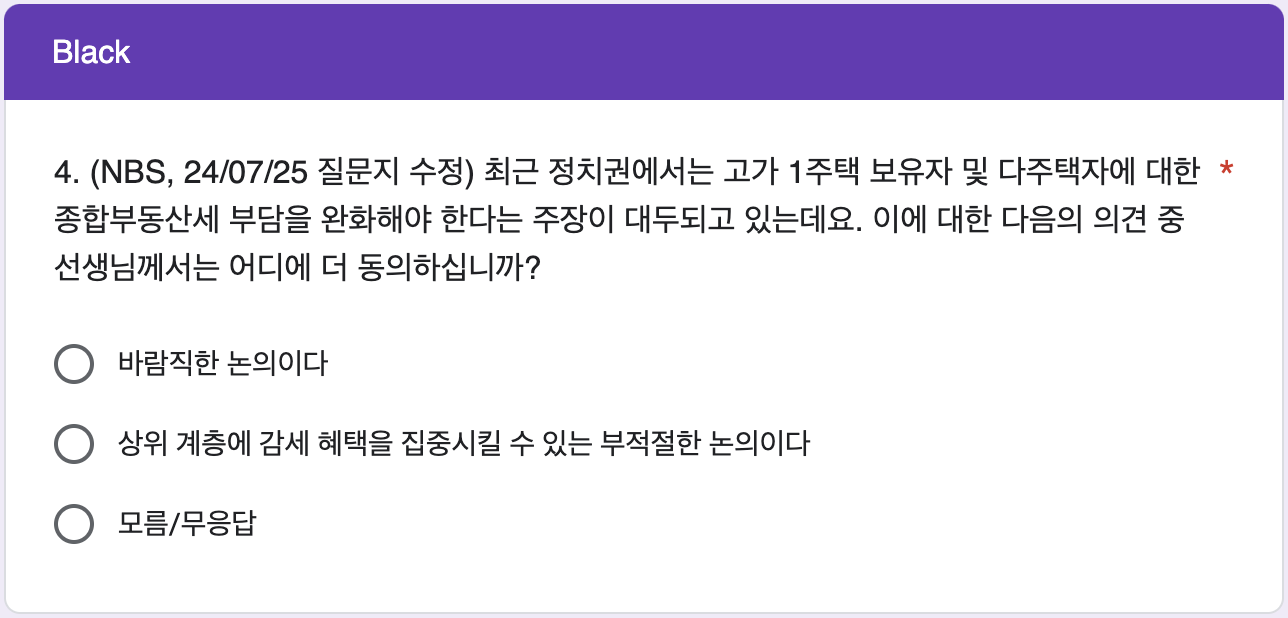
\includegraphics[width=0.67\linewidth]{./pics/Quiz240902_Q4_Black} \end{flushleft}

\subsection{집계}\label{uxc9d1uxacc4}

\begin{longtable}[]{@{}
  >{\raggedright\arraybackslash}p{(\columnwidth - 8\tabcolsep) * \real{0.3023}}
  >{\centering\arraybackslash}p{(\columnwidth - 8\tabcolsep) * \real{0.2326}}
  >{\centering\arraybackslash}p{(\columnwidth - 8\tabcolsep) * \real{0.2326}}
  >{\centering\arraybackslash}p{(\columnwidth - 8\tabcolsep) * \real{0.1628}}
  >{\centering\arraybackslash}p{(\columnwidth - 8\tabcolsep) * \real{0.0698}}@{}}
\toprule\noalign{}
\begin{minipage}[b]{\linewidth}\raggedright
~
\end{minipage} & \begin{minipage}[b]{\linewidth}\centering
바람직한 논의이다
\end{minipage} & \begin{minipage}[b]{\linewidth}\centering
부적절한 논의이다
\end{minipage} & \begin{minipage}[b]{\linewidth}\centering
모름/무응답
\end{minipage} & \begin{minipage}[b]{\linewidth}\centering
계
\end{minipage} \\
\midrule\noalign{}
\endhead
\bottomrule\noalign{}
\endlastfoot
\textbf{Red(바람직한 논의에
부연설명)} & 95 & 113 & 84 & 292 \\
\textbf{Black(부적절한 논의에
부연설명)} & 72 & 130 & 82 & 284 \\
\textbf{계} & 167 & 243 & 166 & 576 \\
\end{longtable}

\begin{longtable}[]{@{}
  >{\raggedleft\arraybackslash}p{(\columnwidth - 4\tabcolsep) * \real{0.2361}}
  >{\raggedleft\arraybackslash}p{(\columnwidth - 4\tabcolsep) * \real{0.0694}}
  >{\raggedleft\arraybackslash}p{(\columnwidth - 4\tabcolsep) * \real{0.1389}}@{}}
\caption{Pearson's Chi-squared test: \texttt{.}}\tabularnewline
\toprule\noalign{}
\begin{minipage}[b]{\linewidth}\raggedleft
Test statistic
\end{minipage} & \begin{minipage}[b]{\linewidth}\raggedleft
df
\end{minipage} & \begin{minipage}[b]{\linewidth}\raggedleft
P value
\end{minipage} \\
\midrule\noalign{}
\endfirsthead
\toprule\noalign{}
\begin{minipage}[b]{\linewidth}\raggedleft
Test statistic
\end{minipage} & \begin{minipage}[b]{\linewidth}\raggedleft
df
\end{minipage} & \begin{minipage}[b]{\linewidth}\raggedleft
P value
\end{minipage} \\
\midrule\noalign{}
\endhead
\bottomrule\noalign{}
\endlastfoot
4.271 & 2 & 0.1182 \\
\end{longtable}

Q4의 Red에는 종합부동산세 부담을 완화해야 한다는 주장에 대하여 바람직한 논의라는 쪽에 긍정적인 부연설명을 붙였는데, 292명이 응답한 가운데 95명이 ``바람직한 논의이다''라는 반응을 보이고, 113명이 ``부적절한 논의이다''라는 반응을 보입니다.

Black에는 같은 주장에 대하여 부적절한 논의라는 쪽에 부정적인 부연설명을 붙였는데, 284명이 응답한 가운데 72명이 ``바람직한 논의이다''라는 반응을 보이고, 130명이 ``부적절한 논의이다''라는 반응을 보입니다.

그리고 ``모름/무응답''에 답한 인원은 Red에 84명, Black 에 82명이 응답하였습니다.

지난 학기 자료들에서 볼 수 있다시피 카이제곱 테스트는 이와 같은 상황에서 부연설명의 유무가 응답에 미치는 영향이 대부분 통계적으로 유의하다는 것을 보여 줍니다.

그런데, 이번 학기는 매우 예외적으로 그렇지 않은 경우가 관찰되었습니다.

카이제곱 통계량은 4.271, 자유도는 2, p-value 는 0.1182으로 부연설명을 어떻게 붙이느냐에 따라 반응이 다르게 나온다는 것을 보여주고 싶었지만 실제로 관찰된 차이는 Q1 \textasciitilde{} Q3와 마찬가지로 통계적으로 유의한 수준은 아닙니다.

여기서 부연설명이 응답에 영향을 끼치지 않는다고 가정해 봅시다.

그렇다면 Red, Black 의 응답은 Q1\textasciitilde Q3 에서와 같이 랜덤화 효과에 의하여 통계적으로 유의한 차이를 보이지 않을 것입니다.

그런데 실제로 관찰된 카이제곱 통계값과 P-value 는 통계적으로 유의한 차이를 보여 주지 못하는 수준입니다.

따라서 부연설명이 영향을 끼치지 않는다는 가정을 받아들일 수밖에 없게 되었습니다.

지난 학기 자료들이 모두 통계적으로 유의한 차이를 보여 주었던 것과는 달리 이번 학기에 유독 통계적으로 유의한 차이를 보이지 않는 이유는 무엇일까요?

\subsection{\% 비교.}\label{uxbe44uxad50.}

\begin{longtable}[]{@{}
  >{\raggedright\arraybackslash}p{(\columnwidth - 8\tabcolsep) * \real{0.2955}}
  >{\centering\arraybackslash}p{(\columnwidth - 8\tabcolsep) * \real{0.2273}}
  >{\centering\arraybackslash}p{(\columnwidth - 8\tabcolsep) * \real{0.2273}}
  >{\centering\arraybackslash}p{(\columnwidth - 8\tabcolsep) * \real{0.1591}}
  >{\centering\arraybackslash}p{(\columnwidth - 8\tabcolsep) * \real{0.0909}}@{}}
\toprule\noalign{}
\begin{minipage}[b]{\linewidth}\raggedright
~
\end{minipage} & \begin{minipage}[b]{\linewidth}\centering
바람직한 논의이다
\end{minipage} & \begin{minipage}[b]{\linewidth}\centering
부적절한 논의이다
\end{minipage} & \begin{minipage}[b]{\linewidth}\centering
모름/무응답
\end{minipage} & \begin{minipage}[b]{\linewidth}\centering
계
\end{minipage} \\
\midrule\noalign{}
\endhead
\bottomrule\noalign{}
\endlastfoot
\textbf{Red(바람직한 논의에
부연설명)} & 32.5 & 38.7 & 28.8 & 100.0 \\
\textbf{Black(부적절한 논의에
부연설명)} & 25.4 & 45.8 & 28.9 & 100.0 \\
\end{longtable}

``바람직한 논의이다''에 부연설명을 붙인 Red에서 ``바람직한 논의이다''라고 응답하는 사람들의 백분율, 32.5(\%)은 ``부적절한 논의이다''에 부연설명을 붙인 Black 에서 ``바람직한 논의이다''라고 응답하는 사람들의 백분율, 25.4(\%) 보다 높습니다.

반면 ``부적절한 논의이다''에 부연설명을 붙인 Black 에서 ``부적절한 논의이다''라고 응답하는 사람들의 백분율, 45.8(\%)은 Red 에서 ``부적절한 논의이다''라고 응답하는 사람들의 백분율, 38.7(\%) 보다 높습니다.

부연설명을 어디에 붙이느냐에 따라 반응이 치우치는 것을 알 수 있지만 p-value 가 보여주듯이 \textbf{그 차이가 통계적으로 유의한 수준은 아닌 것}입니다.

\subsection{Mosaic Plot}\label{mosaic-plot}

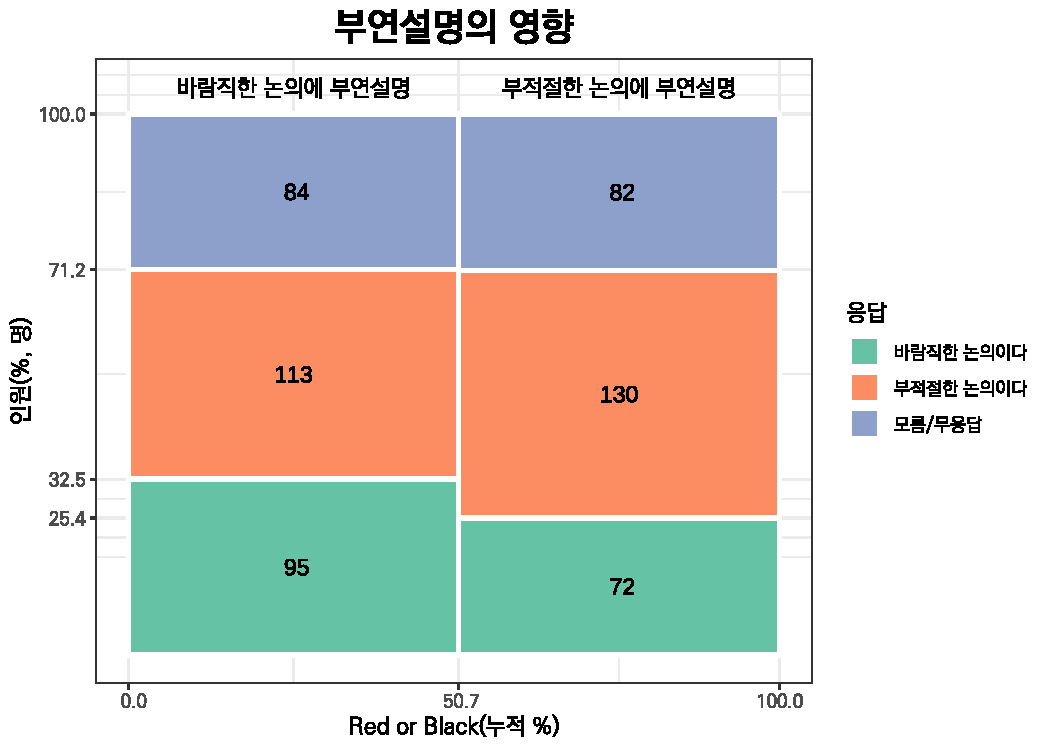
\includegraphics{_main_files/figure-latex/unnamed-chunk-26-1.pdf}

Mosaic Plot 은 이 집계결과를 시각적으로 잘 보여줍니다.

``바람직한 논의이다''에 부연설명을 붙인 Red 에서 ``바람직힌 논의이다''라고 응답한 백분율이 ``부적절한 논의이다''에 부연설명을 붙인 Black 에서 ``바람직한 논의이다''라고 응답한 백분율보다 높고, Black 에서 ``부적절한 논의이다''라고 응답한 백분율은 Red 에서 ``부적절한 논의이다''라고 응답한 백분율보다 월등히 높습니다.

\section{마감 시간으로부터 제출 시간의 분포}\label{uxb9c8uxac10-uxc2dcuxac04uxc73cuxb85cuxbd80uxd130-uxc81cuxcd9c-uxc2dcuxac04uxc758-uxbd84uxd3ec}

\subsection{분포표}\label{uxbd84uxd3ecuxd45c-1}

\begin{longtable}[]{@{}
  >{\raggedright\arraybackslash}p{(\columnwidth - 30\tabcolsep) * \real{0.0863}}
  >{\raggedleft\arraybackslash}p{(\columnwidth - 30\tabcolsep) * \real{0.0576}}
  >{\raggedleft\arraybackslash}p{(\columnwidth - 30\tabcolsep) * \real{0.0576}}
  >{\raggedleft\arraybackslash}p{(\columnwidth - 30\tabcolsep) * \real{0.0576}}
  >{\raggedleft\arraybackslash}p{(\columnwidth - 30\tabcolsep) * \real{0.0576}}
  >{\raggedleft\arraybackslash}p{(\columnwidth - 30\tabcolsep) * \real{0.0576}}
  >{\raggedleft\arraybackslash}p{(\columnwidth - 30\tabcolsep) * \real{0.0576}}
  >{\raggedleft\arraybackslash}p{(\columnwidth - 30\tabcolsep) * \real{0.0576}}
  >{\raggedleft\arraybackslash}p{(\columnwidth - 30\tabcolsep) * \real{0.0576}}
  >{\raggedleft\arraybackslash}p{(\columnwidth - 30\tabcolsep) * \real{0.0576}}
  >{\raggedleft\arraybackslash}p{(\columnwidth - 30\tabcolsep) * \real{0.0647}}
  >{\raggedleft\arraybackslash}p{(\columnwidth - 30\tabcolsep) * \real{0.0719}}
  >{\raggedleft\arraybackslash}p{(\columnwidth - 30\tabcolsep) * \real{0.0719}}
  >{\raggedleft\arraybackslash}p{(\columnwidth - 30\tabcolsep) * \real{0.0719}}
  >{\raggedleft\arraybackslash}p{(\columnwidth - 30\tabcolsep) * \real{0.0719}}
  >{\centering\arraybackslash}p{(\columnwidth - 30\tabcolsep) * \real{0.0432}}@{}}
\caption{일 단위}\tabularnewline
\toprule\noalign{}
\begin{minipage}[b]{\linewidth}\raggedright
~
\end{minipage} & \begin{minipage}[b]{\linewidth}\raggedleft
{[}0,1{]}
\end{minipage} & \begin{minipage}[b]{\linewidth}\raggedleft
(1,2{]}
\end{minipage} & \begin{minipage}[b]{\linewidth}\raggedleft
(2,3{]}
\end{minipage} & \begin{minipage}[b]{\linewidth}\raggedleft
(3,4{]}
\end{minipage} & \begin{minipage}[b]{\linewidth}\raggedleft
(4,5{]}
\end{minipage} & \begin{minipage}[b]{\linewidth}\raggedleft
(5,6{]}
\end{minipage} & \begin{minipage}[b]{\linewidth}\raggedleft
(6,7{]}
\end{minipage} & \begin{minipage}[b]{\linewidth}\raggedleft
(7,8{]}
\end{minipage} & \begin{minipage}[b]{\linewidth}\raggedleft
(8,9{]}
\end{minipage} & \begin{minipage}[b]{\linewidth}\raggedleft
(9,10{]}
\end{minipage} & \begin{minipage}[b]{\linewidth}\raggedleft
(10,11{]}
\end{minipage} & \begin{minipage}[b]{\linewidth}\raggedleft
(11,12{]}
\end{minipage} & \begin{minipage}[b]{\linewidth}\raggedleft
(12,13{]}
\end{minipage} & \begin{minipage}[b]{\linewidth}\raggedleft
(13,14{]}
\end{minipage} & \begin{minipage}[b]{\linewidth}\centering
계
\end{minipage} \\
\midrule\noalign{}
\endfirsthead
\toprule\noalign{}
\begin{minipage}[b]{\linewidth}\raggedright
~
\end{minipage} & \begin{minipage}[b]{\linewidth}\raggedleft
{[}0,1{]}
\end{minipage} & \begin{minipage}[b]{\linewidth}\raggedleft
(1,2{]}
\end{minipage} & \begin{minipage}[b]{\linewidth}\raggedleft
(2,3{]}
\end{minipage} & \begin{minipage}[b]{\linewidth}\raggedleft
(3,4{]}
\end{minipage} & \begin{minipage}[b]{\linewidth}\raggedleft
(4,5{]}
\end{minipage} & \begin{minipage}[b]{\linewidth}\raggedleft
(5,6{]}
\end{minipage} & \begin{minipage}[b]{\linewidth}\raggedleft
(6,7{]}
\end{minipage} & \begin{minipage}[b]{\linewidth}\raggedleft
(7,8{]}
\end{minipage} & \begin{minipage}[b]{\linewidth}\raggedleft
(8,9{]}
\end{minipage} & \begin{minipage}[b]{\linewidth}\raggedleft
(9,10{]}
\end{minipage} & \begin{minipage}[b]{\linewidth}\raggedleft
(10,11{]}
\end{minipage} & \begin{minipage}[b]{\linewidth}\raggedleft
(11,12{]}
\end{minipage} & \begin{minipage}[b]{\linewidth}\raggedleft
(12,13{]}
\end{minipage} & \begin{minipage}[b]{\linewidth}\raggedleft
(13,14{]}
\end{minipage} & \begin{minipage}[b]{\linewidth}\centering
계
\end{minipage} \\
\midrule\noalign{}
\endhead
\bottomrule\noalign{}
\endlastfoot
\textbf{Red} & 46 & 11 & 6 & 11 & 6 & 14 & 10 & 42 & 21 & 19 & 15 & 30 & 35 & 26 & 292 \\
\textbf{Black} & 35 & 10 & 6 & 7 & 5 & 12 & 12 & 34 & 22 & 17 & 26 & 37 & 29 & 32 & 284 \\
\textbf{계} & 81 & 21 & 12 & 18 & 11 & 26 & 22 & 76 & 43 & 36 & 41 & 67 & 64 & 58 & 576 \\
\end{longtable}

분포표로부터 두 가지 문제를 살펴보겠습니다.

첫째, 날마다 고르게 제출하는가?

둘째, Red, Black 간에 통계적으로 유의한 차이가 있는가?

각 문제를 살펴보기 위해서는 분포표의 일부분을 대상으로 카이제곱 테스트를 수행합니다.

\subsection{날마다 고르게 제출하는가?}\label{uxb0a0uxb9c8uxb2e4-uxace0uxb974uxac8c-uxc81cuxcd9cuxd558uxb294uxac00}

\begin{longtable}[]{@{}
  >{\raggedleft\arraybackslash}p{(\columnwidth - 26\tabcolsep) * \real{0.0661}}
  >{\raggedleft\arraybackslash}p{(\columnwidth - 26\tabcolsep) * \real{0.0661}}
  >{\raggedleft\arraybackslash}p{(\columnwidth - 26\tabcolsep) * \real{0.0661}}
  >{\raggedleft\arraybackslash}p{(\columnwidth - 26\tabcolsep) * \real{0.0661}}
  >{\raggedleft\arraybackslash}p{(\columnwidth - 26\tabcolsep) * \real{0.0661}}
  >{\raggedleft\arraybackslash}p{(\columnwidth - 26\tabcolsep) * \real{0.0661}}
  >{\raggedleft\arraybackslash}p{(\columnwidth - 26\tabcolsep) * \real{0.0661}}
  >{\raggedleft\arraybackslash}p{(\columnwidth - 26\tabcolsep) * \real{0.0661}}
  >{\raggedleft\arraybackslash}p{(\columnwidth - 26\tabcolsep) * \real{0.0661}}
  >{\raggedleft\arraybackslash}p{(\columnwidth - 26\tabcolsep) * \real{0.0744}}
  >{\raggedleft\arraybackslash}p{(\columnwidth - 26\tabcolsep) * \real{0.0826}}
  >{\raggedleft\arraybackslash}p{(\columnwidth - 26\tabcolsep) * \real{0.0826}}
  >{\raggedleft\arraybackslash}p{(\columnwidth - 26\tabcolsep) * \real{0.0826}}
  >{\raggedleft\arraybackslash}p{(\columnwidth - 26\tabcolsep) * \real{0.0826}}@{}}
\toprule\noalign{}
\begin{minipage}[b]{\linewidth}\raggedleft
{[}0,1{]}
\end{minipage} & \begin{minipage}[b]{\linewidth}\raggedleft
(1,2{]}
\end{minipage} & \begin{minipage}[b]{\linewidth}\raggedleft
(2,3{]}
\end{minipage} & \begin{minipage}[b]{\linewidth}\raggedleft
(3,4{]}
\end{minipage} & \begin{minipage}[b]{\linewidth}\raggedleft
(4,5{]}
\end{minipage} & \begin{minipage}[b]{\linewidth}\raggedleft
(5,6{]}
\end{minipage} & \begin{minipage}[b]{\linewidth}\raggedleft
(6,7{]}
\end{minipage} & \begin{minipage}[b]{\linewidth}\raggedleft
(7,8{]}
\end{minipage} & \begin{minipage}[b]{\linewidth}\raggedleft
(8,9{]}
\end{minipage} & \begin{minipage}[b]{\linewidth}\raggedleft
(9,10{]}
\end{minipage} & \begin{minipage}[b]{\linewidth}\raggedleft
(10,11{]}
\end{minipage} & \begin{minipage}[b]{\linewidth}\raggedleft
(11,12{]}
\end{minipage} & \begin{minipage}[b]{\linewidth}\raggedleft
(12,13{]}
\end{minipage} & \begin{minipage}[b]{\linewidth}\raggedleft
(13,14{]}
\end{minipage} \\
\midrule\noalign{}
\endhead
\bottomrule\noalign{}
\endlastfoot
81 & 21 & 12 & 18 & 11 & 26 & 22 & 76 & 43 & 36 & 41 & 67 & 64 & 58 \\
\end{longtable}

\begin{longtable}[]{@{}
  >{\raggedleft\arraybackslash}p{(\columnwidth - 4\tabcolsep) * \real{0.2361}}
  >{\raggedleft\arraybackslash}p{(\columnwidth - 4\tabcolsep) * \real{0.0694}}
  >{\raggedleft\arraybackslash}p{(\columnwidth - 4\tabcolsep) * \real{0.2500}}@{}}
\caption{Chi-squared test for given probabilities: \texttt{.}}\tabularnewline
\toprule\noalign{}
\begin{minipage}[b]{\linewidth}\raggedleft
Test statistic
\end{minipage} & \begin{minipage}[b]{\linewidth}\raggedleft
df
\end{minipage} & \begin{minipage}[b]{\linewidth}\raggedleft
P value
\end{minipage} \\
\midrule\noalign{}
\endfirsthead
\toprule\noalign{}
\begin{minipage}[b]{\linewidth}\raggedleft
Test statistic
\end{minipage} & \begin{minipage}[b]{\linewidth}\raggedleft
df
\end{minipage} & \begin{minipage}[b]{\linewidth}\raggedleft
P value
\end{minipage} \\
\midrule\noalign{}
\endhead
\bottomrule\noalign{}
\endlastfoot
184.8 & 13 & 1.766e-32 * * * \\
\end{longtable}

날마다 고르게 제출하는지 알아 보았습니다.

분포표의 ``계''행에서 '계'열을 제외하고 카이제곱테스트를 수행합니다.

분포표 만으로도 쉽게 파악할 수 있지만 카이제곱테스트가 명확히 해 줍니다.

카이제곱 통계량은 184.812, 자유도는 13, p-value 는 1.8e-32 이므로 결코 고르게 제출한다고 말할 수 없겠습니다.

막대그래프로 살펴 보겠습니다.

\subsection{막대그래프}\label{uxb9c9uxb300uxadf8uxb798uxd504-1}

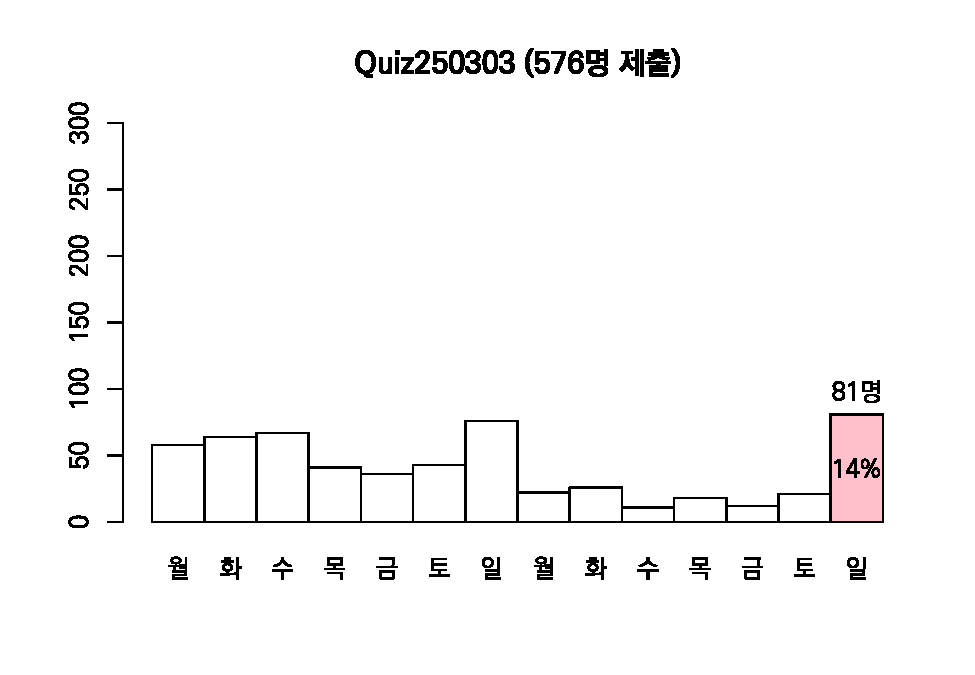
\includegraphics{_main_files/figure-latex/unnamed-chunk-30-1.pdf}

막대그래프는 총 제출인원 576(명) 중에 81(명), 14(\%)가 마감일에 몰리는 것을 보여주고 있습니다.

\subsection{Red, Black 간에 닮았는가?}\label{red-black-uxac04uxc5d0-uxb2eeuxc558uxb294uxac00}

\begin{longtable}[]{@{}
  >{\raggedright\arraybackslash}p{(\columnwidth - 28\tabcolsep) * \real{0.0902}}
  >{\raggedleft\arraybackslash}p{(\columnwidth - 28\tabcolsep) * \real{0.0602}}
  >{\raggedleft\arraybackslash}p{(\columnwidth - 28\tabcolsep) * \real{0.0602}}
  >{\raggedleft\arraybackslash}p{(\columnwidth - 28\tabcolsep) * \real{0.0602}}
  >{\raggedleft\arraybackslash}p{(\columnwidth - 28\tabcolsep) * \real{0.0602}}
  >{\raggedleft\arraybackslash}p{(\columnwidth - 28\tabcolsep) * \real{0.0602}}
  >{\raggedleft\arraybackslash}p{(\columnwidth - 28\tabcolsep) * \real{0.0602}}
  >{\raggedleft\arraybackslash}p{(\columnwidth - 28\tabcolsep) * \real{0.0602}}
  >{\raggedleft\arraybackslash}p{(\columnwidth - 28\tabcolsep) * \real{0.0602}}
  >{\raggedleft\arraybackslash}p{(\columnwidth - 28\tabcolsep) * \real{0.0602}}
  >{\raggedleft\arraybackslash}p{(\columnwidth - 28\tabcolsep) * \real{0.0677}}
  >{\raggedleft\arraybackslash}p{(\columnwidth - 28\tabcolsep) * \real{0.0752}}
  >{\raggedleft\arraybackslash}p{(\columnwidth - 28\tabcolsep) * \real{0.0752}}
  >{\raggedleft\arraybackslash}p{(\columnwidth - 28\tabcolsep) * \real{0.0752}}
  >{\raggedleft\arraybackslash}p{(\columnwidth - 28\tabcolsep) * \real{0.0752}}@{}}
\toprule\noalign{}
\begin{minipage}[b]{\linewidth}\raggedright
~
\end{minipage} & \begin{minipage}[b]{\linewidth}\raggedleft
{[}0,1{]}
\end{minipage} & \begin{minipage}[b]{\linewidth}\raggedleft
(1,2{]}
\end{minipage} & \begin{minipage}[b]{\linewidth}\raggedleft
(2,3{]}
\end{minipage} & \begin{minipage}[b]{\linewidth}\raggedleft
(3,4{]}
\end{minipage} & \begin{minipage}[b]{\linewidth}\raggedleft
(4,5{]}
\end{minipage} & \begin{minipage}[b]{\linewidth}\raggedleft
(5,6{]}
\end{minipage} & \begin{minipage}[b]{\linewidth}\raggedleft
(6,7{]}
\end{minipage} & \begin{minipage}[b]{\linewidth}\raggedleft
(7,8{]}
\end{minipage} & \begin{minipage}[b]{\linewidth}\raggedleft
(8,9{]}
\end{minipage} & \begin{minipage}[b]{\linewidth}\raggedleft
(9,10{]}
\end{minipage} & \begin{minipage}[b]{\linewidth}\raggedleft
(10,11{]}
\end{minipage} & \begin{minipage}[b]{\linewidth}\raggedleft
(11,12{]}
\end{minipage} & \begin{minipage}[b]{\linewidth}\raggedleft
(12,13{]}
\end{minipage} & \begin{minipage}[b]{\linewidth}\raggedleft
(13,14{]}
\end{minipage} \\
\midrule\noalign{}
\endhead
\bottomrule\noalign{}
\endlastfoot
\textbf{Red} & 46 & 11 & 6 & 11 & 6 & 14 & 10 & 42 & 21 & 19 & 15 & 30 & 35 & 26 \\
\textbf{Black} & 35 & 10 & 6 & 7 & 5 & 12 & 12 & 34 & 22 & 17 & 26 & 37 & 29 & 32 \\
\end{longtable}

\begin{longtable}[]{@{}
  >{\raggedleft\arraybackslash}p{(\columnwidth - 4\tabcolsep) * \real{0.2361}}
  >{\raggedleft\arraybackslash}p{(\columnwidth - 4\tabcolsep) * \real{0.0694}}
  >{\raggedleft\arraybackslash}p{(\columnwidth - 4\tabcolsep) * \real{0.1389}}@{}}
\caption{Pearson's Chi-squared test: \texttt{.}}\tabularnewline
\toprule\noalign{}
\begin{minipage}[b]{\linewidth}\raggedleft
Test statistic
\end{minipage} & \begin{minipage}[b]{\linewidth}\raggedleft
df
\end{minipage} & \begin{minipage}[b]{\linewidth}\raggedleft
P value
\end{minipage} \\
\midrule\noalign{}
\endfirsthead
\toprule\noalign{}
\begin{minipage}[b]{\linewidth}\raggedleft
Test statistic
\end{minipage} & \begin{minipage}[b]{\linewidth}\raggedleft
df
\end{minipage} & \begin{minipage}[b]{\linewidth}\raggedleft
P value
\end{minipage} \\
\midrule\noalign{}
\endhead
\bottomrule\noalign{}
\endlastfoot
8.59 & 13 & 0.8032 \\
\end{longtable}

제출시간의 분포가 Red, Black 간에 닮았는지 알아 보았습니다.

이번에는 분포표의 첫번째와 두번째 행, '계'열을 제외한 나머지 열에 대해서 카이제곱테스트를 수행합니다.

카이제곱 통계량은 8.590, 자유도는 13, p-value 는 0.8032 이므로 제출 시간의 분포는 Red, Black 간에 통계적으로 유의한 차이가 관찰되지 않습니다.

이 사실을 Mosaic Plot 을 이용하여 시각적으로 살펴보겠습니다.

닮았다고 느껴지나요?

\subsection{Mosaic Plot}\label{mosaic-plot-1}

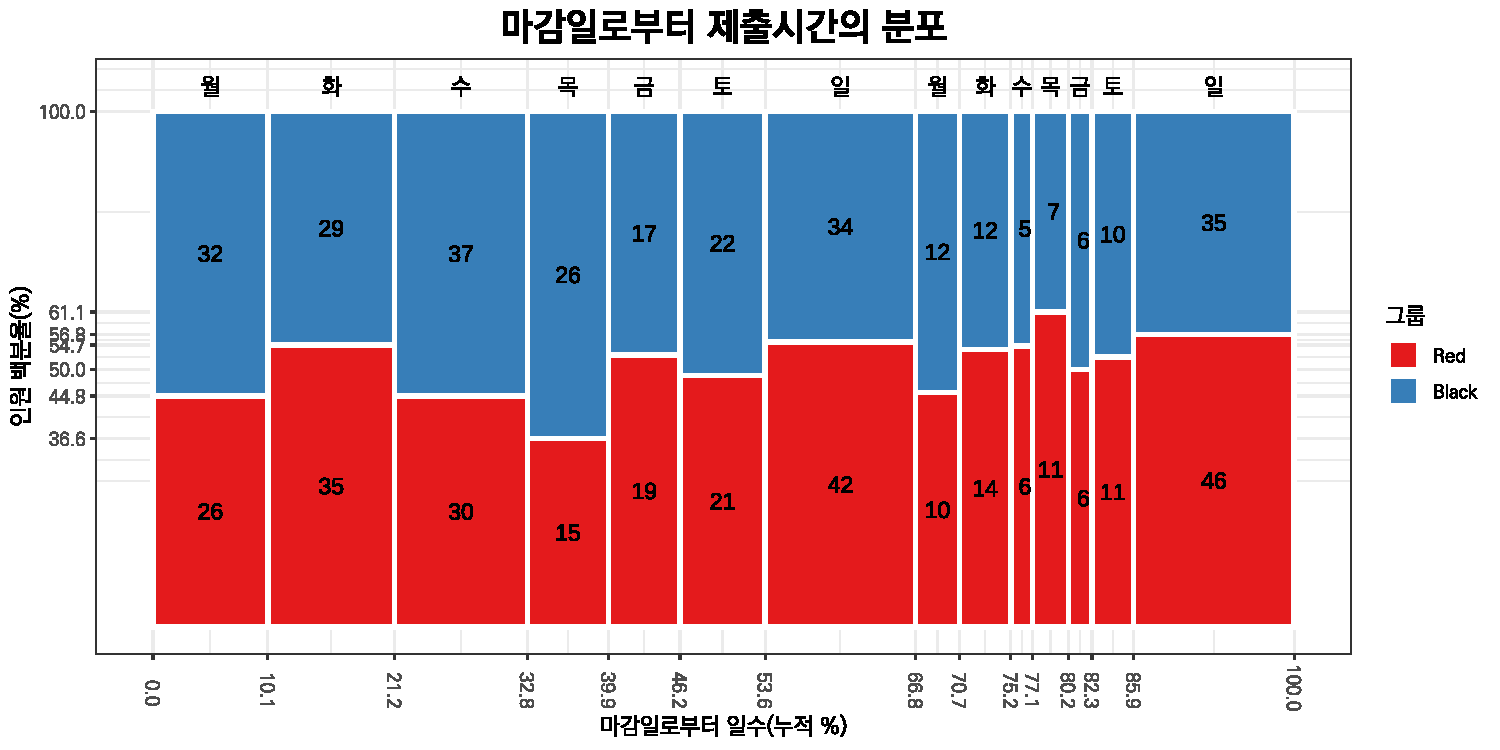
\includegraphics{_main_files/figure-latex/unnamed-chunk-32-1.pdf}

\chapter{2주차 데이터 실험 집계}\label{uxc8fcuxcc28-uxb370uxc774uxd130-uxc2e4uxd5d8-uxc9d1uxacc4-1}

\section{실험의 목적}\label{uxc2e4uxd5d8uxc758-uxbaa9uxc801-1}

2주차 구글 예습 설문지 집계결과를 분석합니다.

Q1\textasciitilde Q6에서는 랜덤화의 효과로 Red, Black 이 얼마나 닮았는지 알아봅니다.

Q7에서는 같은 눈속임 그래프인데 원형그래프의 각도를 속일 떄(Red)와 막대그래프의 높이를 속일 때(Black) 오류를 지각하는 데 차이가 있는지 알아봅니다.

끝으로 제출시간의 분포가 날마다 고른지, Red, Black 간에는 닮았는지 알아봅니다.

\subsection{Red, Black을 잘못 표시한 사람들}\label{red-blackuxc744-uxc798uxbabb-uxd45cuxc2dcuxd55c-uxc0acuxb78cuxb4e4-1}

\begin{longtable}[]{@{}
  >{\centering\arraybackslash}p{(\columnwidth - 6\tabcolsep) * \real{0.3056}}
  >{\centering\arraybackslash}p{(\columnwidth - 6\tabcolsep) * \real{0.1528}}
  >{\centering\arraybackslash}p{(\columnwidth - 6\tabcolsep) * \real{0.2083}}
  >{\centering\arraybackslash}p{(\columnwidth - 6\tabcolsep) * \real{0.2083}}@{}}
\toprule\noalign{}
\begin{minipage}[b]{\linewidth}\centering
제출시간
\end{minipage} & \begin{minipage}[b]{\linewidth}\centering
학번
\end{minipage} & \begin{minipage}[b]{\linewidth}\centering
랜덤화출석부
\end{minipage} & \begin{minipage}[b]{\linewidth}\centering
구글예습퀴즈
\end{minipage} \\
\midrule\noalign{}
\endhead
\bottomrule\noalign{}
\endlastfoot
2025-03-11 21:44:18 & 20223501 & Red & Black \\
2025-03-12 01:12:52 & 20246792 & Black & Red \\
2025-03-12 02:27:14 & 20242601 & Red & Black \\
2025-03-13 02:06:41 & 20246737 & Red & Black \\
2025-03-13 19:03:57 & 20241216 & Red & Black \\
2025-03-14 09:32:05 & 20241022 & Black & Red \\
2025-03-14 10:22:29 & 20231725 & Red & Black \\
2025-03-14 15:07:21 & 20243233 & Black & Red \\
2025-03-15 15:21:53 & 20213033 & Red & Black \\
2025-03-15 22:20:27 & 20241201 & Red & Black \\
2025-03-15 22:46:42 & 20243720 & Red & Black \\
2025-03-16 15:31:37 & 20223329 & Black & Red \\
2025-03-16 17:32:57 & 20211021 & Black & Red \\
2025-03-16 19:50:32 & 20241011 & Red & Black \\
2025-03-16 20:56:30 & 20213040 & Red & Black \\
2025-03-16 23:10:55 & 20241028 & Black & Red \\
2025-03-17 21:59:54 & 20242960 & Black & Red \\
2025-03-20 11:14:21 & 20246272 & Black & Red \\
2025-03-20 14:54:36 & 20246923 & Black & Red \\
2025-03-20 20:52:14 & 20242949 & Black & Red \\
2025-03-22 00:55:57 & 20246606 & Black & Red \\
2025-03-23 11:51:35 & 20242585 & Red & Black \\
2025-03-23 14:27:48 & 20243513 & Black & Red \\
2025-03-23 19:53:42 & 20227107 & Red & Black \\
\end{longtable}

\begin{longtable}[]{@{}
  >{\raggedright\arraybackslash}p{(\columnwidth - 4\tabcolsep) * \real{0.3611}}
  >{\centering\arraybackslash}p{(\columnwidth - 4\tabcolsep) * \real{0.2778}}
  >{\centering\arraybackslash}p{(\columnwidth - 4\tabcolsep) * \real{0.3056}}@{}}
\toprule\noalign{}
\begin{minipage}[b]{\linewidth}\raggedright
~
\end{minipage} & \begin{minipage}[b]{\linewidth}\centering
Red(구글예습퀴즈)
\end{minipage} & \begin{minipage}[b]{\linewidth}\centering
Black(구글예습퀴즈)
\end{minipage} \\
\midrule\noalign{}
\endhead
\bottomrule\noalign{}
\endlastfoot
\textbf{Red(랜덤화출석부)} & 268 & 12 \\
\textbf{Black(랜덤화출석부)} & 12 & 269 \\
\textbf{계} & 280 & 281 \\
\end{longtable}

랜덤화출석부에 있는 Red, Black 과 실제 구글설문에 올린 Red, Black 이 다른 사람들의 수효는 24명입니다.

Red를 Black 이라고 한 사람이 12명, Black 을 Red 라고 한 사람이 12명입니다.

두 가지 방법으로 분석합니다.

우선 Red, Black 을 잘못 선택한 24명을 랜덤하게 둘로 나누면 어느 한 쪽 집단에 들어갈 기대인원은 24명을 둘로 나눈 12(명)이고, 표준오차는 24의 제곱근에 1/2을 곱해 준 2.4명이 됩니다.

실제로 Red를 Black 이라고 한 사람수, 12명이나 Black 을 Red 라고 한 사람수, 12명은 기대인원으로부터 표준오차 범위 안에 아주 잘 들어갑니다.

두 번째 분석 방법은 확률을 계산해 보는 것입니다.

Red, Black 을 잘못 선택한 24명을 랜덤하게 둘로 나눌 때, 실제로 관찰된 12명 이상이나 12명이하로 잘못 선택한 사람수가 나올 가능성은 얼마나 되는가 입니다.

이 경우 공평한 동전던지기를 확률 법칙으로 표현한 이항분포로부터 계산할 수 있습니다.

시행횟수가 24이고 한 번 시행에서 성공확률이 1/2 인 이항분포에서 성공횟수가 12이하이거나 12이상을 관찰할 확률은 1.161입니다.

공평한 동전 던지기에서 앞면이 12개 이하 나오는 확률은 12개 이상 나오는 확률과 같기 때문에 사실상 한쪽만 계산해서 2배 해 주면 됩니다.

이 값을 p-value 라고 하는데, p-value가 0.05보다 작을 때 \textbf{통계적으로 유의한 차이를 관찰}하였다고 말합니다.

즉, 공평한 동전을 던지는 것과 같은 과정이라고 가정하였을 때 실제로 관찰된 값들이 가정으로부터 얼마나 떨어져 있는지를 표현한 것입니다.

0.05, 즉 1/20은 이런 실험을 스무 번 정도 반복하면 1번 나올 정도로 드문 사건을 의미합니다.

즉 가정이 타당하다면 나오기 힘든 결과라는 것입니다.

그런데 Red, Black 을 잘못 표시한 사람들의 분포에서 관찰된 p-value 는 0.05와는 비교도 안될 정도로 큰 값입니다.

따라서 두 집단이 랜덤화 효과가 작동하여 \textbf{통계적으로 유의한 차이를 보이지 않는다}고 할 수 있습니다.

\subsection{응답인원의 Red, Black}\label{uxc751uxb2f5uxc778uxc6d0uxc758-red-black-1}

Red 로 응답한 인원은 280명, Black 에 응답한 인원은 281명입니다.

전체 응답인원 561 명을 랜덤하게 둘로 나눌 때 어느 한 쪽의 기대인원은 전체 응답인원의 절반인 280.5명이고, 표준오차는 전체 응답인원의 제곱근에 1/2을 곱해 준 11.8 명입니다.

따라서 Red, Black 각 그룹에 관찰된 인원은 기대인원으로부터 표준오차 범위, 혹은 두배의 표준오차 범위 안에 들어갑니다.

\section{Q1. 춘추전국시대에 국가통계관리의 중요성 강조}\label{q1.-uxcd98uxcd94uxc804uxad6duxc2dcuxb300uxc5d0-uxad6duxac00uxd1b5uxacc4uxad00uxb9acuxc758-uxc911uxc694uxc131-uxac15uxc870}

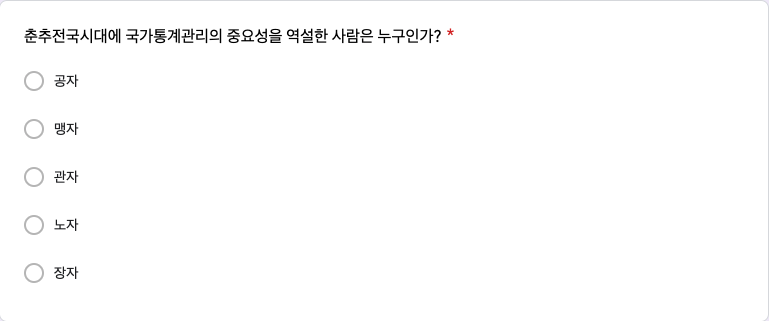
\includegraphics[width=0.75\linewidth]{./pics/Quiz210309_01}

\subsection{관자(집계표)}\label{uxad00uxc790uxc9d1uxacc4uxd45c}

\begin{longtable}[]{@{}
  >{\raggedright\arraybackslash}p{(\columnwidth - 12\tabcolsep) * \real{0.1667}}
  >{\centering\arraybackslash}p{(\columnwidth - 12\tabcolsep) * \real{0.0972}}
  >{\centering\arraybackslash}p{(\columnwidth - 12\tabcolsep) * \real{0.0972}}
  >{\centering\arraybackslash}p{(\columnwidth - 12\tabcolsep) * \real{0.0972}}
  >{\centering\arraybackslash}p{(\columnwidth - 12\tabcolsep) * \real{0.0972}}
  >{\centering\arraybackslash}p{(\columnwidth - 12\tabcolsep) * \real{0.0972}}
  >{\centering\arraybackslash}p{(\columnwidth - 12\tabcolsep) * \real{0.0972}}@{}}
\toprule\noalign{}
\begin{minipage}[b]{\linewidth}\raggedright
~
\end{minipage} & \begin{minipage}[b]{\linewidth}\centering
공자
\end{minipage} & \begin{minipage}[b]{\linewidth}\centering
맹자
\end{minipage} & \begin{minipage}[b]{\linewidth}\centering
관자
\end{minipage} & \begin{minipage}[b]{\linewidth}\centering
노자
\end{minipage} & \begin{minipage}[b]{\linewidth}\centering
장자
\end{minipage} & \begin{minipage}[b]{\linewidth}\centering
계
\end{minipage} \\
\midrule\noalign{}
\endhead
\bottomrule\noalign{}
\endlastfoot
\textbf{Red} & 40 & 9 & 224 & 8 & 1 & 282 \\
\textbf{Black} & 25 & 17 & 223 & 11 & 5 & 281 \\
\textbf{계} & 65 & 26 & 447 & 19 & 6 & 563 \\
\end{longtable}

\begin{longtable}[]{@{}
  >{\raggedleft\arraybackslash}p{(\columnwidth - 4\tabcolsep) * \real{0.2361}}
  >{\raggedleft\arraybackslash}p{(\columnwidth - 4\tabcolsep) * \real{0.0694}}
  >{\raggedleft\arraybackslash}p{(\columnwidth - 4\tabcolsep) * \real{0.1389}}@{}}
\caption{Pearson's Chi-squared test with simulated p-value
(based on 2000 replicates): \texttt{.}}\tabularnewline
\toprule\noalign{}
\begin{minipage}[b]{\linewidth}\raggedleft
Test statistic
\end{minipage} & \begin{minipage}[b]{\linewidth}\raggedleft
df
\end{minipage} & \begin{minipage}[b]{\linewidth}\raggedleft
P value
\end{minipage} \\
\midrule\noalign{}
\endfirsthead
\toprule\noalign{}
\begin{minipage}[b]{\linewidth}\raggedleft
Test statistic
\end{minipage} & \begin{minipage}[b]{\linewidth}\raggedleft
df
\end{minipage} & \begin{minipage}[b]{\linewidth}\raggedleft
P value
\end{minipage} \\
\midrule\noalign{}
\endhead
\bottomrule\noalign{}
\endlastfoot
9.064 & NA & 0.05197 \\
\end{longtable}

Q1의 집계 결과가 Red, Black 간에 통계적으로 유의한 차이가 있는지 알아보기 위하여 카이제곱 테스트를 수행하였습니다.

그 결과 카이제곱 통계량은 9.06, 자유도는 NA , p-value 는 0.0520이므로 Red, Black 간에 통계적으로 유의한 차이를 보이지 않습니다.

실제로 닮은 게 느껴집니까?

\subsection{관자(\%)}\label{uxad00uxc790}

\begin{longtable}[]{@{}
  >{\centering\arraybackslash}p{(\columnwidth - 10\tabcolsep) * \real{0.0972}}
  >{\centering\arraybackslash}p{(\columnwidth - 10\tabcolsep) * \real{0.0972}}
  >{\centering\arraybackslash}p{(\columnwidth - 10\tabcolsep) * \real{0.0972}}
  >{\centering\arraybackslash}p{(\columnwidth - 10\tabcolsep) * \real{0.0972}}
  >{\centering\arraybackslash}p{(\columnwidth - 10\tabcolsep) * \real{0.0972}}
  >{\centering\arraybackslash}p{(\columnwidth - 10\tabcolsep) * \real{0.1111}}@{}}
\toprule\noalign{}
\begin{minipage}[b]{\linewidth}\centering
공자
\end{minipage} & \begin{minipage}[b]{\linewidth}\centering
맹자
\end{minipage} & \begin{minipage}[b]{\linewidth}\centering
관자
\end{minipage} & \begin{minipage}[b]{\linewidth}\centering
노자
\end{minipage} & \begin{minipage}[b]{\linewidth}\centering
장자
\end{minipage} & \begin{minipage}[b]{\linewidth}\centering
계
\end{minipage} \\
\midrule\noalign{}
\endhead
\bottomrule\noalign{}
\endlastfoot
11.5 & 4.6 & 79.4 & 3.4 & 1.1 & 100.0 \\
\end{longtable}

정답률은 Red, Black 을 합하여 계산하는데, 79.4(\%) 입니다.

\section{Q2. 국가정책을 수립하는 데 통계의 역할}\label{q2.-uxad6duxac00uxc815uxcc45uxc744-uxc218uxb9bduxd558uxb294-uxb370-uxd1b5uxacc4uxc758-uxc5eduxd560}

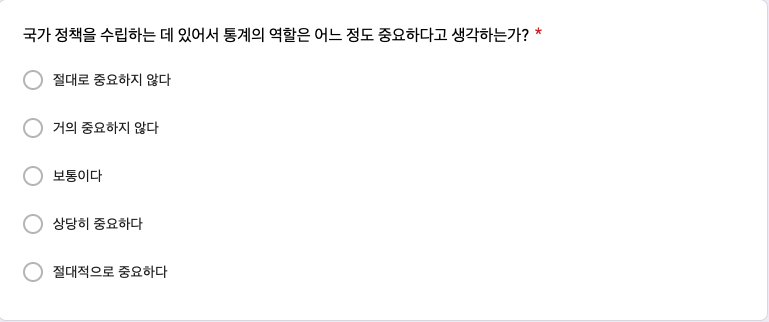
\includegraphics[width=0.75\linewidth]{./pics/Quiz210309_02}

\subsection{통계의 중요성(집계표)}\label{uxd1b5uxacc4uxc758-uxc911uxc694uxc131uxc9d1uxacc4uxd45c}

\begin{longtable}[]{@{}
  >{\raggedright\arraybackslash}p{(\columnwidth - 12\tabcolsep) * \real{0.1062}}
  >{\centering\arraybackslash}p{(\columnwidth - 12\tabcolsep) * \real{0.2035}}
  >{\centering\arraybackslash}p{(\columnwidth - 12\tabcolsep) * \real{0.1858}}
  >{\centering\arraybackslash}p{(\columnwidth - 12\tabcolsep) * \real{0.0973}}
  >{\centering\arraybackslash}p{(\columnwidth - 12\tabcolsep) * \real{0.1593}}
  >{\centering\arraybackslash}p{(\columnwidth - 12\tabcolsep) * \real{0.1947}}
  >{\centering\arraybackslash}p{(\columnwidth - 12\tabcolsep) * \real{0.0531}}@{}}
\toprule\noalign{}
\begin{minipage}[b]{\linewidth}\raggedright
~
\end{minipage} & \begin{minipage}[b]{\linewidth}\centering
절대로 중요하지 않다
\end{minipage} & \begin{minipage}[b]{\linewidth}\centering
거의 중요하지 않다
\end{minipage} & \begin{minipage}[b]{\linewidth}\centering
보통이다
\end{minipage} & \begin{minipage}[b]{\linewidth}\centering
상당히 중요하다
\end{minipage} & \begin{minipage}[b]{\linewidth}\centering
절대적으로 중요하다
\end{minipage} & \begin{minipage}[b]{\linewidth}\centering
계
\end{minipage} \\
\midrule\noalign{}
\endhead
\bottomrule\noalign{}
\endlastfoot
\textbf{Red} & 0 & 2 & 9 & 94 & 177 & 282 \\
\textbf{Black} & 2 & 4 & 9 & 94 & 172 & 281 \\
\textbf{계} & 2 & 6 & 18 & 188 & 349 & 563 \\
\end{longtable}

\begin{longtable}[]{@{}
  >{\raggedleft\arraybackslash}p{(\columnwidth - 4\tabcolsep) * \real{0.2361}}
  >{\raggedleft\arraybackslash}p{(\columnwidth - 4\tabcolsep) * \real{0.0694}}
  >{\raggedleft\arraybackslash}p{(\columnwidth - 4\tabcolsep) * \real{0.1389}}@{}}
\caption{Pearson's Chi-squared test with simulated p-value
(based on 2000 replicates): \texttt{.}}\tabularnewline
\toprule\noalign{}
\begin{minipage}[b]{\linewidth}\raggedleft
Test statistic
\end{minipage} & \begin{minipage}[b]{\linewidth}\raggedleft
df
\end{minipage} & \begin{minipage}[b]{\linewidth}\raggedleft
P value
\end{minipage} \\
\midrule\noalign{}
\endfirsthead
\toprule\noalign{}
\begin{minipage}[b]{\linewidth}\raggedleft
Test statistic
\end{minipage} & \begin{minipage}[b]{\linewidth}\raggedleft
df
\end{minipage} & \begin{minipage}[b]{\linewidth}\raggedleft
P value
\end{minipage} \\
\midrule\noalign{}
\endhead
\bottomrule\noalign{}
\endlastfoot
2.056 & NA & 0.6687 \\
\end{longtable}

Q2의 집계 결과가 Red, Black 간에 통계적으로 유의한 차이가 있는지 알아보기 위하여 카이제곱 테스트를 수행하였습니다.

그 결과 카이제곱 통계량은 2.056, 자유도는 NA, p-value 는 0.6687이므로 Red, Black 간에 통계적으로 유의한 차이를 보이지 않습니다.

실제로 닮은 게 느껴집니까?

\subsection{통계의 중요성(\%)}\label{uxd1b5uxacc4uxc758-uxc911uxc694uxc131}

\begin{longtable}[]{@{}
  >{\centering\arraybackslash}p{(\columnwidth - 10\tabcolsep) * \real{0.2212}}
  >{\centering\arraybackslash}p{(\columnwidth - 10\tabcolsep) * \real{0.2019}}
  >{\centering\arraybackslash}p{(\columnwidth - 10\tabcolsep) * \real{0.1058}}
  >{\centering\arraybackslash}p{(\columnwidth - 10\tabcolsep) * \real{0.1731}}
  >{\centering\arraybackslash}p{(\columnwidth - 10\tabcolsep) * \real{0.2115}}
  >{\centering\arraybackslash}p{(\columnwidth - 10\tabcolsep) * \real{0.0865}}@{}}
\toprule\noalign{}
\begin{minipage}[b]{\linewidth}\centering
절대로 중요하지 않다
\end{minipage} & \begin{minipage}[b]{\linewidth}\centering
거의 중요하지 않다
\end{minipage} & \begin{minipage}[b]{\linewidth}\centering
보통이다
\end{minipage} & \begin{minipage}[b]{\linewidth}\centering
상당히 중요하다
\end{minipage} & \begin{minipage}[b]{\linewidth}\centering
절대적으로 중요하다
\end{minipage} & \begin{minipage}[b]{\linewidth}\centering
계
\end{minipage} \\
\midrule\noalign{}
\endhead
\bottomrule\noalign{}
\endlastfoot
0.36 & 1.07 & 3.20 & 33.39 & 61.99 & 100.00 \\
\end{longtable}

정답률은 Red, Black 을 합하여 계산하는데, 62.0(\%) 입니다.

\section{Q3. 우리나라 생산가능인구 감소 시기}\label{q3.-uxc6b0uxb9acuxb098uxb77c-uxc0dduxc0b0uxac00uxb2a5uxc778uxad6c-uxac10uxc18c-uxc2dcuxae30}

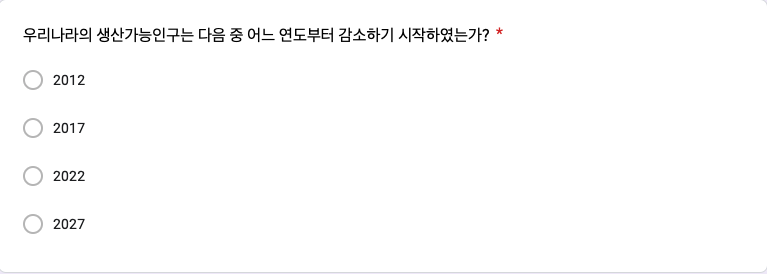
\includegraphics[width=0.75\linewidth]{./pics/Quiz210309_03}

\subsection{생산가능인구 감소 시기(집계표)}\label{uxc0dduxc0b0uxac00uxb2a5uxc778uxad6c-uxac10uxc18c-uxc2dcuxae30uxc9d1uxacc4uxd45c}

\begin{longtable}[]{@{}
  >{\raggedright\arraybackslash}p{(\columnwidth - 10\tabcolsep) * \real{0.1667}}
  >{\raggedleft\arraybackslash}p{(\columnwidth - 10\tabcolsep) * \real{0.0972}}
  >{\raggedleft\arraybackslash}p{(\columnwidth - 10\tabcolsep) * \real{0.0972}}
  >{\raggedleft\arraybackslash}p{(\columnwidth - 10\tabcolsep) * \real{0.0972}}
  >{\raggedleft\arraybackslash}p{(\columnwidth - 10\tabcolsep) * \real{0.0972}}
  >{\centering\arraybackslash}p{(\columnwidth - 10\tabcolsep) * \real{0.0972}}@{}}
\toprule\noalign{}
\begin{minipage}[b]{\linewidth}\raggedright
~
\end{minipage} & \begin{minipage}[b]{\linewidth}\raggedleft
2012
\end{minipage} & \begin{minipage}[b]{\linewidth}\raggedleft
2017
\end{minipage} & \begin{minipage}[b]{\linewidth}\raggedleft
2022
\end{minipage} & \begin{minipage}[b]{\linewidth}\raggedleft
2027
\end{minipage} & \begin{minipage}[b]{\linewidth}\centering
계
\end{minipage} \\
\midrule\noalign{}
\endhead
\bottomrule\noalign{}
\endlastfoot
\textbf{Red} & 31 & 224 & 23 & 4 & 282 \\
\textbf{Black} & 23 & 227 & 25 & 6 & 281 \\
\textbf{계} & 54 & 451 & 48 & 10 & 563 \\
\end{longtable}

\begin{longtable}[]{@{}
  >{\raggedleft\arraybackslash}p{(\columnwidth - 4\tabcolsep) * \real{0.2361}}
  >{\raggedleft\arraybackslash}p{(\columnwidth - 4\tabcolsep) * \real{0.0694}}
  >{\raggedleft\arraybackslash}p{(\columnwidth - 4\tabcolsep) * \real{0.1389}}@{}}
\caption{Pearson's Chi-squared test: \texttt{.}}\tabularnewline
\toprule\noalign{}
\begin{minipage}[b]{\linewidth}\raggedleft
Test statistic
\end{minipage} & \begin{minipage}[b]{\linewidth}\raggedleft
df
\end{minipage} & \begin{minipage}[b]{\linewidth}\raggedleft
P value
\end{minipage} \\
\midrule\noalign{}
\endfirsthead
\toprule\noalign{}
\begin{minipage}[b]{\linewidth}\raggedleft
Test statistic
\end{minipage} & \begin{minipage}[b]{\linewidth}\raggedleft
df
\end{minipage} & \begin{minipage}[b]{\linewidth}\raggedleft
P value
\end{minipage} \\
\midrule\noalign{}
\endhead
\bottomrule\noalign{}
\endlastfoot
1.687 & 3 & 0.6399 \\
\end{longtable}

Q3의 집계 결과가 Red, Black 간에 통계적으로 유의한 차이가 있는지 알아보기 위하여 카이제곱 테스트를 수행하였습니다.

그 결과 카이제곱 통계량은 1.687, 자유도는 3, p-value 는 0.6399이므로 Red, Black 간에 통계적으로 유의한 차이를 보이지 않습니다.

실제로 닮은 게 느껴집니까?

\subsection{생산가능인구 감소 시기(\%)}\label{uxc0dduxc0b0uxac00uxb2a5uxc778uxad6c-uxac10uxc18c-uxc2dcuxae30}

\begin{longtable}[]{@{}
  >{\raggedleft\arraybackslash}p{(\columnwidth - 8\tabcolsep) * \real{0.0972}}
  >{\raggedleft\arraybackslash}p{(\columnwidth - 8\tabcolsep) * \real{0.0972}}
  >{\raggedleft\arraybackslash}p{(\columnwidth - 8\tabcolsep) * \real{0.0972}}
  >{\raggedleft\arraybackslash}p{(\columnwidth - 8\tabcolsep) * \real{0.0972}}
  >{\centering\arraybackslash}p{(\columnwidth - 8\tabcolsep) * \real{0.1111}}@{}}
\toprule\noalign{}
\begin{minipage}[b]{\linewidth}\raggedleft
2012
\end{minipage} & \begin{minipage}[b]{\linewidth}\raggedleft
2017
\end{minipage} & \begin{minipage}[b]{\linewidth}\raggedleft
2022
\end{minipage} & \begin{minipage}[b]{\linewidth}\raggedleft
2027
\end{minipage} & \begin{minipage}[b]{\linewidth}\centering
계
\end{minipage} \\
\midrule\noalign{}
\endhead
\bottomrule\noalign{}
\endlastfoot
9.6 & 80.1 & 8.5 & 1.8 & 100.0 \\
\end{longtable}

정답률은 Red, Black 을 합하여 계산하는데, 80.1(\%) 입니다.

\section{Q4. 우리나라 총인구 최대 시기}\label{q4.-uxc6b0uxb9acuxb098uxb77c-uxcd1duxc778uxad6c-uxcd5cuxb300-uxc2dcuxae30}


\includegraphics[width=0.75\linewidth]{./pics/Quiz230308_Q4}

\subsection{총인구 최대 시기(집계표)}\label{uxcd1duxc778uxad6c-uxcd5cuxb300-uxc2dcuxae30uxc9d1uxacc4uxd45c}

\begin{longtable}[]{@{}
  >{\raggedright\arraybackslash}p{(\columnwidth - 10\tabcolsep) * \real{0.1667}}
  >{\raggedleft\arraybackslash}p{(\columnwidth - 10\tabcolsep) * \real{0.0972}}
  >{\raggedleft\arraybackslash}p{(\columnwidth - 10\tabcolsep) * \real{0.0972}}
  >{\raggedleft\arraybackslash}p{(\columnwidth - 10\tabcolsep) * \real{0.0972}}
  >{\raggedleft\arraybackslash}p{(\columnwidth - 10\tabcolsep) * \real{0.0972}}
  >{\centering\arraybackslash}p{(\columnwidth - 10\tabcolsep) * \real{0.0972}}@{}}
\toprule\noalign{}
\begin{minipage}[b]{\linewidth}\raggedright
~
\end{minipage} & \begin{minipage}[b]{\linewidth}\raggedleft
2018
\end{minipage} & \begin{minipage}[b]{\linewidth}\raggedleft
2019
\end{minipage} & \begin{minipage}[b]{\linewidth}\raggedleft
2020
\end{minipage} & \begin{minipage}[b]{\linewidth}\raggedleft
2021
\end{minipage} & \begin{minipage}[b]{\linewidth}\centering
계
\end{minipage} \\
\midrule\noalign{}
\endhead
\bottomrule\noalign{}
\endlastfoot
\textbf{Red} & 47 & 27 & 205 & 3 & 282 \\
\textbf{Black} & 29 & 27 & 215 & 10 & 281 \\
\textbf{계} & 76 & 54 & 420 & 13 & 563 \\
\end{longtable}

\begin{longtable}[]{@{}
  >{\raggedleft\arraybackslash}p{(\columnwidth - 4\tabcolsep) * \real{0.2361}}
  >{\raggedleft\arraybackslash}p{(\columnwidth - 4\tabcolsep) * \real{0.0694}}
  >{\raggedleft\arraybackslash}p{(\columnwidth - 4\tabcolsep) * \real{0.1667}}@{}}
\caption{Pearson's Chi-squared test with simulated p-value
(based on 2000 replicates): \texttt{.}}\tabularnewline
\toprule\noalign{}
\begin{minipage}[b]{\linewidth}\raggedleft
Test statistic
\end{minipage} & \begin{minipage}[b]{\linewidth}\raggedleft
df
\end{minipage} & \begin{minipage}[b]{\linewidth}\raggedleft
P value
\end{minipage} \\
\midrule\noalign{}
\endfirsthead
\toprule\noalign{}
\begin{minipage}[b]{\linewidth}\raggedleft
Test statistic
\end{minipage} & \begin{minipage}[b]{\linewidth}\raggedleft
df
\end{minipage} & \begin{minipage}[b]{\linewidth}\raggedleft
P value
\end{minipage} \\
\midrule\noalign{}
\endhead
\bottomrule\noalign{}
\endlastfoot
8.269 & NA & 0.03248 * \\
\end{longtable}

Q4의 집계 결과가 Red, Black 간에 통계적으로 유의한 차이가 있는지 알아보기 위하여 카이제곱 테스트를 수행하였습니다.

그 결과 카이제곱 통계량은 8.269, 자유도는 NA, p-value 는 0.0325이므로 Red, Black 간에 통계적으로 유의한 차이를 보이고 있습니다.

\subsection{총인구 최대 시기(\%)}\label{uxcd1duxc778uxad6c-uxcd5cuxb300-uxc2dcuxae30}

\begin{longtable}[]{@{}
  >{\raggedleft\arraybackslash}p{(\columnwidth - 8\tabcolsep) * \real{0.0972}}
  >{\raggedleft\arraybackslash}p{(\columnwidth - 8\tabcolsep) * \real{0.0972}}
  >{\raggedleft\arraybackslash}p{(\columnwidth - 8\tabcolsep) * \real{0.0972}}
  >{\raggedleft\arraybackslash}p{(\columnwidth - 8\tabcolsep) * \real{0.0972}}
  >{\centering\arraybackslash}p{(\columnwidth - 8\tabcolsep) * \real{0.1111}}@{}}
\toprule\noalign{}
\begin{minipage}[b]{\linewidth}\raggedleft
2018
\end{minipage} & \begin{minipage}[b]{\linewidth}\raggedleft
2019
\end{minipage} & \begin{minipage}[b]{\linewidth}\raggedleft
2020
\end{minipage} & \begin{minipage}[b]{\linewidth}\raggedleft
2021
\end{minipage} & \begin{minipage}[b]{\linewidth}\centering
계
\end{minipage} \\
\midrule\noalign{}
\endhead
\bottomrule\noalign{}
\endlastfoot
13.5 & 9.6 & 74.6 & 2.3 & 100.0 \\
\end{longtable}

정답률은 Red, Black 을 합하여 계산하는데, 74.6(\%) 입니다.

\section{Q5. 소멸위험 단계 개선 지역}\label{q5.-uxc18cuxba78uxc704uxd5d8-uxb2e8uxacc4-uxac1cuxc120-uxc9c0uxc5ed}


\includegraphics[width=0.75\linewidth]{./pics/Quiz230308_Q5}

\subsection{소멸위험 단계 개선 지역(집계표)}\label{uxc18cuxba78uxc704uxd5d8-uxb2e8uxacc4-uxac1cuxc120-uxc9c0uxc5eduxc9d1uxacc4uxd45c}

\begin{longtable}[]{@{}
  >{\raggedright\arraybackslash}p{(\columnwidth - 10\tabcolsep) * \real{0.1667}}
  >{\centering\arraybackslash}p{(\columnwidth - 10\tabcolsep) * \real{0.0972}}
  >{\centering\arraybackslash}p{(\columnwidth - 10\tabcolsep) * \real{0.0972}}
  >{\centering\arraybackslash}p{(\columnwidth - 10\tabcolsep) * \real{0.0972}}
  >{\centering\arraybackslash}p{(\columnwidth - 10\tabcolsep) * \real{0.0972}}
  >{\centering\arraybackslash}p{(\columnwidth - 10\tabcolsep) * \real{0.0972}}@{}}
\toprule\noalign{}
\begin{minipage}[b]{\linewidth}\raggedright
~
\end{minipage} & \begin{minipage}[b]{\linewidth}\centering
서울
\end{minipage} & \begin{minipage}[b]{\linewidth}\centering
경기
\end{minipage} & \begin{minipage}[b]{\linewidth}\centering
세종
\end{minipage} & \begin{minipage}[b]{\linewidth}\centering
제주
\end{minipage} & \begin{minipage}[b]{\linewidth}\centering
계
\end{minipage} \\
\midrule\noalign{}
\endhead
\bottomrule\noalign{}
\endlastfoot
\textbf{Red} & 13 & 14 & 241 & 14 & 282 \\
\textbf{Black} & 9 & 14 & 245 & 13 & 281 \\
\textbf{계} & 22 & 28 & 486 & 27 & 563 \\
\end{longtable}

\begin{longtable}[]{@{}
  >{\raggedleft\arraybackslash}p{(\columnwidth - 4\tabcolsep) * \real{0.2361}}
  >{\raggedleft\arraybackslash}p{(\columnwidth - 4\tabcolsep) * \real{0.0694}}
  >{\raggedleft\arraybackslash}p{(\columnwidth - 4\tabcolsep) * \real{0.1389}}@{}}
\caption{Pearson's Chi-squared test with simulated p-value
(based on 2000 replicates): \texttt{.}}\tabularnewline
\toprule\noalign{}
\begin{minipage}[b]{\linewidth}\raggedleft
Test statistic
\end{minipage} & \begin{minipage}[b]{\linewidth}\raggedleft
df
\end{minipage} & \begin{minipage}[b]{\linewidth}\raggedleft
P value
\end{minipage} \\
\midrule\noalign{}
\endfirsthead
\toprule\noalign{}
\begin{minipage}[b]{\linewidth}\raggedleft
Test statistic
\end{minipage} & \begin{minipage}[b]{\linewidth}\raggedleft
df
\end{minipage} & \begin{minipage}[b]{\linewidth}\raggedleft
P value
\end{minipage} \\
\midrule\noalign{}
\endhead
\bottomrule\noalign{}
\endlastfoot
0.7955 & NA & 0.8691 \\
\end{longtable}

Q5의 집계 결과가 Red, Black 간에 통계적으로 유의한 차이가 있는지 알아보기 위하여 카이제곱 테스트를 수행하였습니다.

그 결과 카이제곱 통계량은 0.795, 자유도는 NA, p-value 는 0.8691이므로 Red, Black 간에 통계적으로 유의한 차이를 보이지 않습니다.

실제로 닮은 게 느껴집니까?

\subsection{소멸위험 단계 개선 지역(\%)}\label{uxc18cuxba78uxc704uxd5d8-uxb2e8uxacc4-uxac1cuxc120-uxc9c0uxc5ed}

\begin{longtable}[]{@{}
  >{\centering\arraybackslash}p{(\columnwidth - 8\tabcolsep) * \real{0.0972}}
  >{\centering\arraybackslash}p{(\columnwidth - 8\tabcolsep) * \real{0.0972}}
  >{\centering\arraybackslash}p{(\columnwidth - 8\tabcolsep) * \real{0.0972}}
  >{\centering\arraybackslash}p{(\columnwidth - 8\tabcolsep) * \real{0.0972}}
  >{\centering\arraybackslash}p{(\columnwidth - 8\tabcolsep) * \real{0.1111}}@{}}
\toprule\noalign{}
\begin{minipage}[b]{\linewidth}\centering
서울
\end{minipage} & \begin{minipage}[b]{\linewidth}\centering
경기
\end{minipage} & \begin{minipage}[b]{\linewidth}\centering
세종
\end{minipage} & \begin{minipage}[b]{\linewidth}\centering
제주
\end{minipage} & \begin{minipage}[b]{\linewidth}\centering
계
\end{minipage} \\
\midrule\noalign{}
\endhead
\bottomrule\noalign{}
\endlastfoot
3.9 & 5.0 & 86.3 & 4.8 & 100.0 \\
\end{longtable}

정답률은 Red, Black 을 합하여 계산하는데, 86.3(\%) 입니다.

\section{Q6. 조출생률과 합계출산율}\label{q6.-uxc870uxcd9cuxc0dduxb960uxacfc-uxd569uxacc4uxcd9cuxc0b0uxc728}

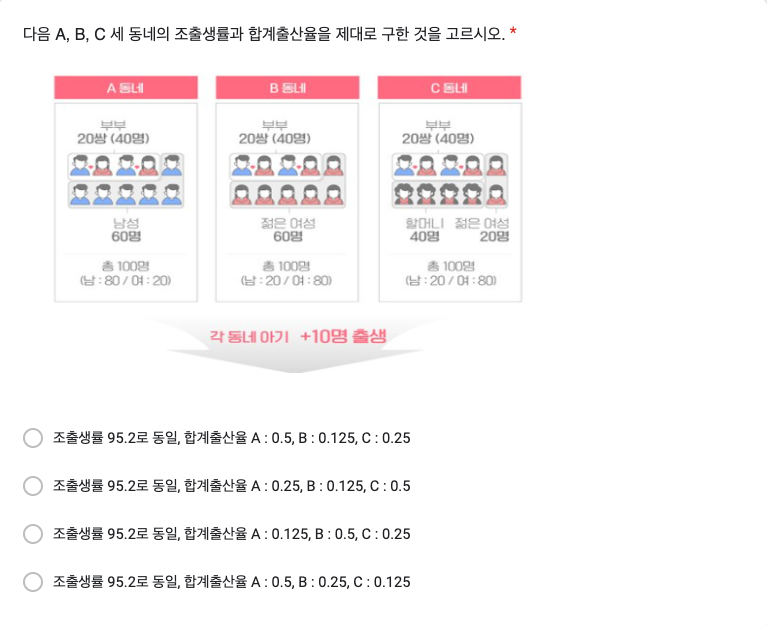
\includegraphics[width=0.75\linewidth]{./pics/Quiz230308_Q6}

\subsection{조출생률과 합계출산율(집계표)}\label{uxc870uxcd9cuxc0dduxb960uxacfc-uxd569uxacc4uxcd9cuxc0b0uxc728uxc9d1uxacc4uxd45c}

\begin{longtable}[]{@{}
  >{\raggedright\arraybackslash}p{(\columnwidth - 10\tabcolsep) * \real{0.0839}}
  >{\centering\arraybackslash}p{(\columnwidth - 10\tabcolsep) * \real{0.2308}}
  >{\centering\arraybackslash}p{(\columnwidth - 10\tabcolsep) * \real{0.1888}}
  >{\centering\arraybackslash}p{(\columnwidth - 10\tabcolsep) * \real{0.2308}}
  >{\centering\arraybackslash}p{(\columnwidth - 10\tabcolsep) * \real{0.2238}}
  >{\centering\arraybackslash}p{(\columnwidth - 10\tabcolsep) * \real{0.0420}}@{}}
\toprule\noalign{}
\begin{minipage}[b]{\linewidth}\raggedright
~
\end{minipage} & \begin{minipage}[b]{\linewidth}\centering
합계출산율 A : 0.5, B : 0.125,
C : 0.25
\end{minipage} & \begin{minipage}[b]{\linewidth}\centering
합계출산율 A : 0.25, B :
0.125, C : 0.5
\end{minipage} & \begin{minipage}[b]{\linewidth}\centering
합계출산율 A : 0.125, B : 0.5,
C : 0.25
\end{minipage} & \begin{minipage}[b]{\linewidth}\centering
합계출산율 A : 0.5, B : 0.25,
C : 0.125
\end{minipage} & \begin{minipage}[b]{\linewidth}\centering
계
\end{minipage} \\
\midrule\noalign{}
\endhead
\bottomrule\noalign{}
\endlastfoot
\textbf{Red} & 163 & 34 & 56 & 29 & 282 \\
\textbf{Black} & 140 & 56 & 48 & 37 & 281 \\
\textbf{계} & 303 & 90 & 104 & 66 & 563 \\
\end{longtable}

\begin{longtable}[]{@{}
  >{\raggedleft\arraybackslash}p{(\columnwidth - 4\tabcolsep) * \real{0.2361}}
  >{\raggedleft\arraybackslash}p{(\columnwidth - 4\tabcolsep) * \real{0.0694}}
  >{\raggedleft\arraybackslash}p{(\columnwidth - 4\tabcolsep) * \real{0.1667}}@{}}
\caption{Pearson's Chi-squared test: \texttt{.}}\tabularnewline
\toprule\noalign{}
\begin{minipage}[b]{\linewidth}\raggedleft
Test statistic
\end{minipage} & \begin{minipage}[b]{\linewidth}\raggedleft
df
\end{minipage} & \begin{minipage}[b]{\linewidth}\raggedleft
P value
\end{minipage} \\
\midrule\noalign{}
\endfirsthead
\toprule\noalign{}
\begin{minipage}[b]{\linewidth}\raggedleft
Test statistic
\end{minipage} & \begin{minipage}[b]{\linewidth}\raggedleft
df
\end{minipage} & \begin{minipage}[b]{\linewidth}\raggedleft
P value
\end{minipage} \\
\midrule\noalign{}
\endhead
\bottomrule\noalign{}
\endlastfoot
8.707 & 3 & 0.03345 * \\
\end{longtable}

Q6의 집계 결과가 Red, Black 간에 통계적으로 유의한 차이가 있는지 알아보기 위하여 카이제곱 테스트를 수행하였습니다.

그 결과 카이제곱 통계량은 8.707, 자유도는 3, p-value 는 0.0335이므로 Red, Black 간에 통계적으로 유의한 차이를 보이고 있습니다.

\subsection{조출생률과 합계출산율(\%)}\label{uxc870uxcd9cuxc0dduxb960uxacfc-uxd569uxacc4uxcd9cuxc0b0uxc728}

\begin{longtable}[]{@{}
  >{\centering\arraybackslash}p{(\columnwidth - 8\tabcolsep) * \real{0.2481}}
  >{\centering\arraybackslash}p{(\columnwidth - 8\tabcolsep) * \real{0.2030}}
  >{\centering\arraybackslash}p{(\columnwidth - 8\tabcolsep) * \real{0.2481}}
  >{\centering\arraybackslash}p{(\columnwidth - 8\tabcolsep) * \real{0.2406}}
  >{\centering\arraybackslash}p{(\columnwidth - 8\tabcolsep) * \real{0.0602}}@{}}
\toprule\noalign{}
\begin{minipage}[b]{\linewidth}\centering
합계출산율 A : 0.5, B : 0.125,
C : 0.25
\end{minipage} & \begin{minipage}[b]{\linewidth}\centering
합계출산율 A : 0.25, B :
0.125, C : 0.5
\end{minipage} & \begin{minipage}[b]{\linewidth}\centering
합계출산율 A : 0.125, B : 0.5,
C : 0.25
\end{minipage} & \begin{minipage}[b]{\linewidth}\centering
합계출산율 A : 0.5, B : 0.25,
C : 0.125
\end{minipage} & \begin{minipage}[b]{\linewidth}\centering
계
\end{minipage} \\
\midrule\noalign{}
\endhead
\bottomrule\noalign{}
\endlastfoot
53.8 & 16.0 & 18.5 & 11.7 & 100.0 \\
\end{longtable}

정답률은 Red, Black 을 합하여 계산하는데, 53.8(\%) 입니다.

\section{Q7. 눈속임 그래프(Cheating Charts)}\label{q7.-uxb208uxc18duxc784-uxadf8uxb798uxd504cheating-charts}

지난 학기까지 앞에 나오는 선지를 고르기 쉽다는 1번효과에 대한 질문을 만들어서 테스트해 왔지만 효과를 검증하기 어려워 문제를 바꿔 보았습니다.

언론방송에서 가끔 원형그래프나 막대그래프를 제시하면서 숫자와 그림이 맞지 않는 경우를 볼 수 있습니다.

여러분들은 그런 경우에 어떻게 인식하는 지 언론기관에서 발표한 눈속임 그래프를 보여줍니다.

Red에는 원형그래프의 각도를 속이고, Black 에는 막대그래프의 높이를 속여 어떤 응답이 나오는 지 살펴보았습니다.

여러분들은 대부분 눈속임 그래프에 속지 않고 있습니다.

언론기관들이 왜 이런 짓들을 하는지 궁금해집니다.

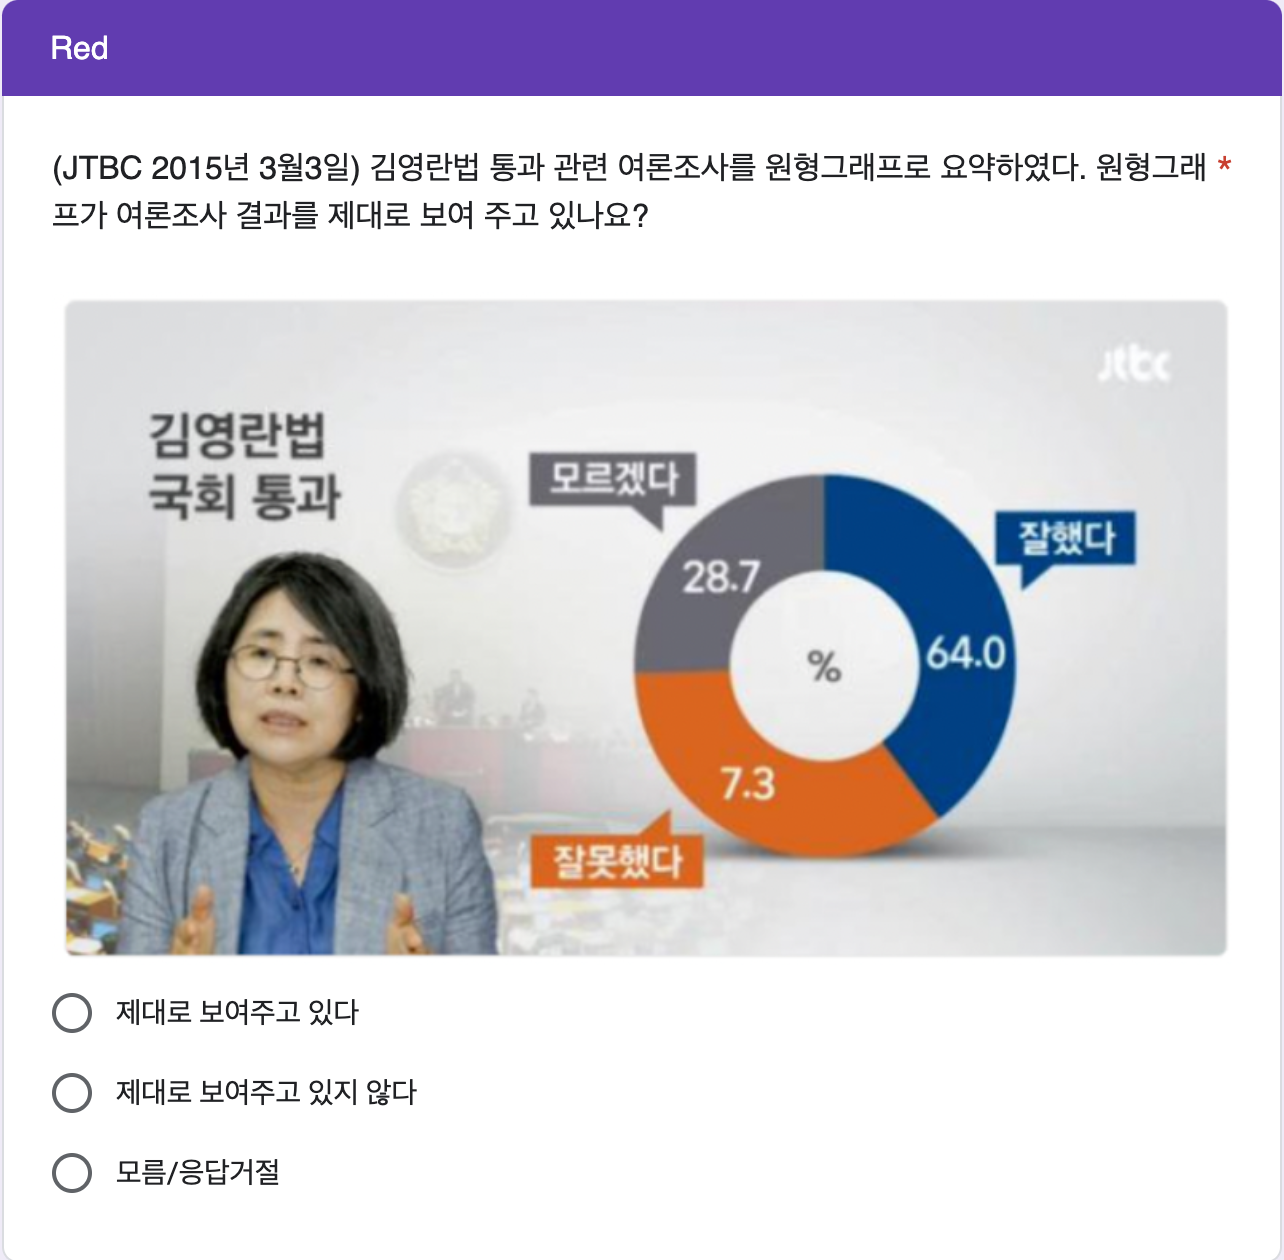
\includegraphics[width=0.67\linewidth]{./pics/Quiz240308_Q7_Red}

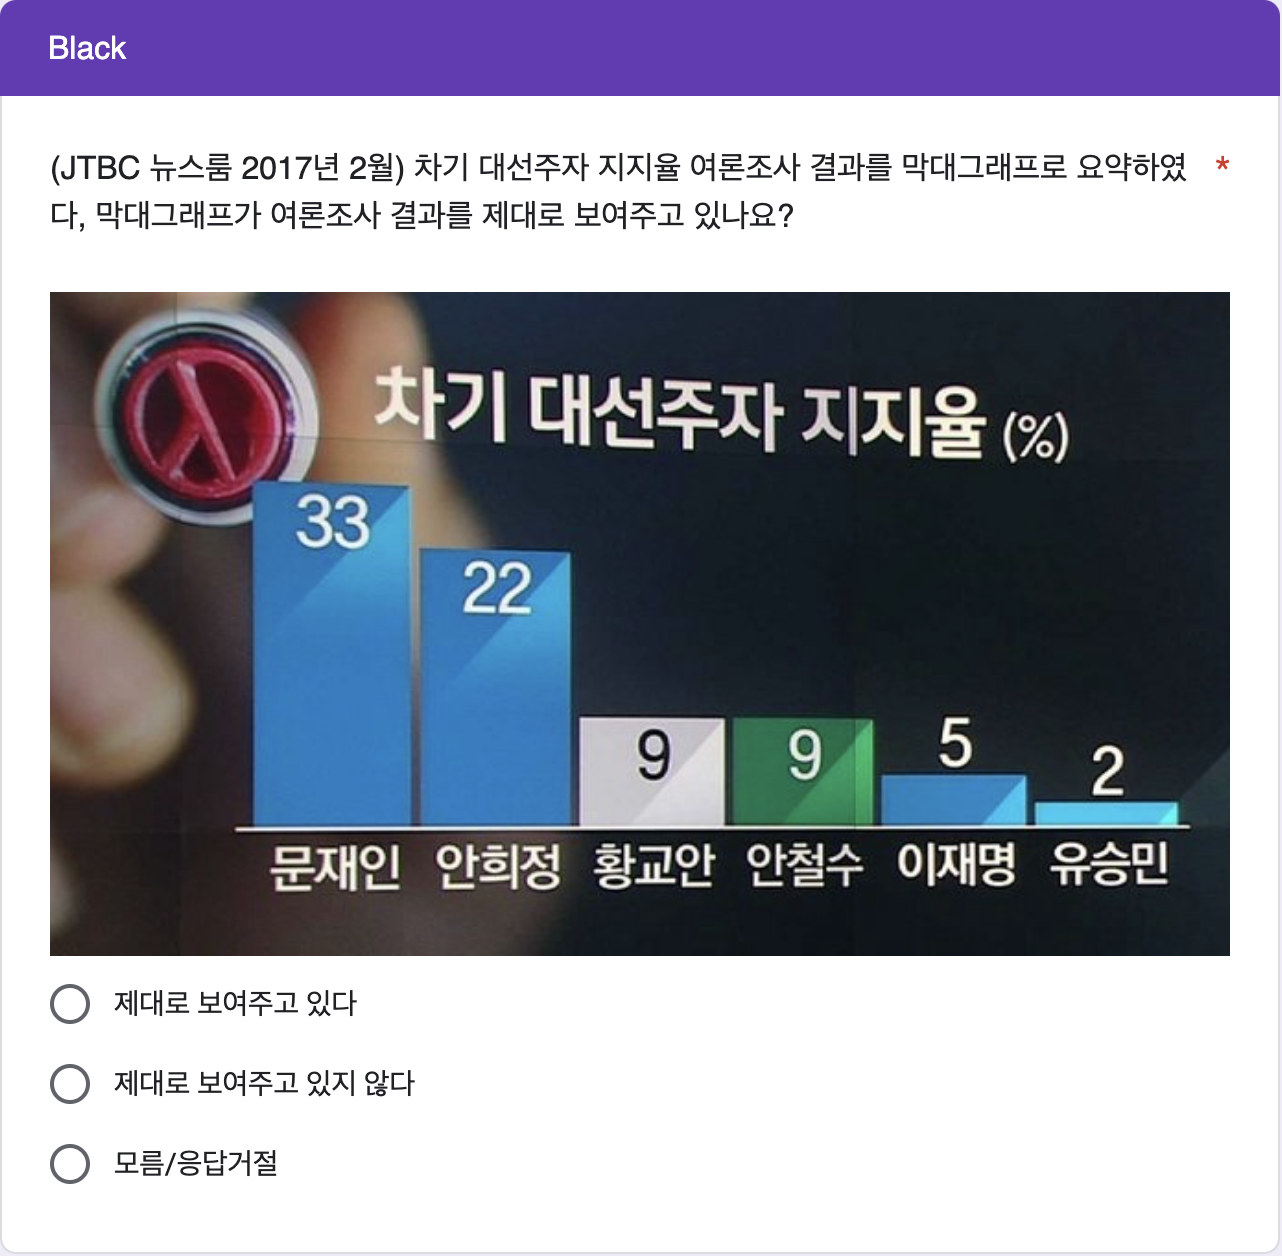
\includegraphics[width=0.67\linewidth]{./pics/Quiz240308_Q7_Black}

\subsection{집계표}\label{uxc9d1uxacc4uxd45c}

\begin{longtable}[]{@{}
  >{\raggedright\arraybackslash}p{(\columnwidth - 8\tabcolsep) * \real{0.3048}}
  >{\centering\arraybackslash}p{(\columnwidth - 8\tabcolsep) * \real{0.2190}}
  >{\centering\arraybackslash}p{(\columnwidth - 8\tabcolsep) * \real{0.2667}}
  >{\centering\arraybackslash}p{(\columnwidth - 8\tabcolsep) * \real{0.1524}}
  >{\centering\arraybackslash}p{(\columnwidth - 8\tabcolsep) * \real{0.0571}}@{}}
\toprule\noalign{}
\begin{minipage}[b]{\linewidth}\raggedright
~
\end{minipage} & \begin{minipage}[b]{\linewidth}\centering
제대로 보여주고 있다
\end{minipage} & \begin{minipage}[b]{\linewidth}\centering
제대로 보여주고 있지 않다
\end{minipage} & \begin{minipage}[b]{\linewidth}\centering
모름/응답거절
\end{minipage} & \begin{minipage}[b]{\linewidth}\centering
계
\end{minipage} \\
\midrule\noalign{}
\endhead
\bottomrule\noalign{}
\endlastfoot
\textbf{Red(김영란법 국회통과)} & 65 & 180 & 37 & 282 \\
\textbf{Black(고위공직자 범죄수사처
설립)} & 100 & 119 & 62 & 281 \\
\textbf{계} & 165 & 299 & 99 & 563 \\
\end{longtable}

\begin{longtable}[]{@{}
  >{\raggedleft\arraybackslash}p{(\columnwidth - 4\tabcolsep) * \real{0.2361}}
  >{\raggedleft\arraybackslash}p{(\columnwidth - 4\tabcolsep) * \real{0.0694}}
  >{\raggedleft\arraybackslash}p{(\columnwidth - 4\tabcolsep) * \real{0.2500}}@{}}
\caption{Pearson's Chi-squared test: \texttt{.}}\tabularnewline
\toprule\noalign{}
\begin{minipage}[b]{\linewidth}\raggedleft
Test statistic
\end{minipage} & \begin{minipage}[b]{\linewidth}\raggedleft
df
\end{minipage} & \begin{minipage}[b]{\linewidth}\raggedleft
P value
\end{minipage} \\
\midrule\noalign{}
\endfirsthead
\toprule\noalign{}
\begin{minipage}[b]{\linewidth}\raggedleft
Test statistic
\end{minipage} & \begin{minipage}[b]{\linewidth}\raggedleft
df
\end{minipage} & \begin{minipage}[b]{\linewidth}\raggedleft
P value
\end{minipage} \\
\midrule\noalign{}
\endhead
\bottomrule\noalign{}
\endlastfoot
26.18 & 2 & 2.065e-06 * * * \\
\end{longtable}

Q7의 Red에는 김영란법 국회통과에 대한 여론조사 결과를 원형그래프로 나타내었는데 잘했다(64\%), 잘못했다(7.3\%), 모르겠다(28.7\%)의 각도를 데이터와 전혀 맞지 않게 왜곡하여 마치 잘했다와 잘못했다의 비율이 거의 대등한 것처럼 각도를 조정하였습니다.

282명이 응답한 가운데 65명이 결과를 ``제대로 보여주고 있다''는 반응을 보이고, 180명이 결과를 ``제대로 보여주고 있지 않다''는 반응을 보입니다.

Black은 2017년 대선의 대선주자 여론조사에서 33\%의 지지율을 기록한 문재인 예비후보와 22\%의 지지율을 기록한 안희정 예비후보의 지지율 막대가 거의 비슷한 것처럼 왜곡하였습니다.

281명이 응답한 가운데 100명이 여론조사 결과를 ''
제대로 보여주고 있다''는 반응을 보이고, 119명이 여론조사 결과를 ``제대로 보여주고 있지 않다''는 반응을 보입니다.

그리고 ``모름/무응답''에 답한 인원은 Red에 37명, Black 에 62명이 었습니다.

카이제곱 테스트는 이와 같은 상황에서 원형그래프를 왜곡할 떄와 막대그래프를 왜곡할 때 인식의 차이가 통계적으로 유의하다는 것을 보여 줍니다.

카이제곱 통계량은 26.180, 자유도는 2, p-value 는 2.1e-06(으)로
그래프의 유형에 따라 눈속임의 인식에 통계적으로 유의한 차이가 관찰된다는 것을 보여줍니다.

여기서 그래프의 유형이 눈속임의 인식에 차이를 주지 않는다고 가정합니다.

랜덤화의 효과로 Red, Black 의 응답은 닮게 마련입니다.

즉, 통계적으로 유의한 차이를 보이지 않게 됩니다.

그러나 실제로 관찰된 카이제곱 통계값의 P-value 는 0.05보다 매우 작은 값입니다.

따라서, 그래프의 유형이 눈속임의 인식에 영향을 끼치지 않는다는 가정은 잘못된 것이죠.

이러한 논증 방식을 귀류법이라고 합니다.

\subsection{\% 비교}\label{uxbe44uxad50}

\begin{longtable}[]{@{}
  >{\raggedright\arraybackslash}p{(\columnwidth - 8\tabcolsep) * \real{0.2991}}
  >{\centering\arraybackslash}p{(\columnwidth - 8\tabcolsep) * \real{0.2150}}
  >{\centering\arraybackslash}p{(\columnwidth - 8\tabcolsep) * \real{0.2617}}
  >{\centering\arraybackslash}p{(\columnwidth - 8\tabcolsep) * \real{0.1495}}
  >{\centering\arraybackslash}p{(\columnwidth - 8\tabcolsep) * \real{0.0748}}@{}}
\toprule\noalign{}
\begin{minipage}[b]{\linewidth}\raggedright
~
\end{minipage} & \begin{minipage}[b]{\linewidth}\centering
제대로 보여주고 있다
\end{minipage} & \begin{minipage}[b]{\linewidth}\centering
제대로 보여주고 있지 않다
\end{minipage} & \begin{minipage}[b]{\linewidth}\centering
모름/응답거절
\end{minipage} & \begin{minipage}[b]{\linewidth}\centering
계
\end{minipage} \\
\midrule\noalign{}
\endhead
\bottomrule\noalign{}
\endlastfoot
\textbf{Red(김영란법 국회통과)} & 23.0 & 63.8 & 13.1 & 100.0 \\
\textbf{Black(고위공직자 범죄수사처
설립)} & 35.6 & 42.3 & 22.1 & 100.0 \\
\end{longtable}

원형그래프의 각도를 왜곡한 Red에서 여론조사 결과를 ``제대로 보여주고 있다''고 응답하는 사람들의 백분율, 23.0(\%)은 ``제대로 보여주고 있지 않다''고 응답하는 사람들의 백분율, 63.8(\%) 보다 매우 낮습니다.

반면 막대그래프의 높이를 왜곡한 Black에서 여론조사 결과를 ``제대로 보여주고 있다''고 응답하는 사람들의 백분율, 35.6(\%)은 ``제대로 보여주고 있지 않다''고 응답하는 사람들의 백분율, 42.3(\%) 보다 적습니다.

원형그래프에서 눈속임을 지각하는 백분율이 막대그래프에서 눈속임을 지각하는 백분율보다 훨씬 높게 나타나고 있습니다.

원형그래프의 각도를 속이느냐, 막대그래프의 높이를 속이느냐에 따라 반응이 달라진다는 것을 잘 알 수 있습니다.

\subsection{Mosaic Plot}\label{mosaic-plot-2}

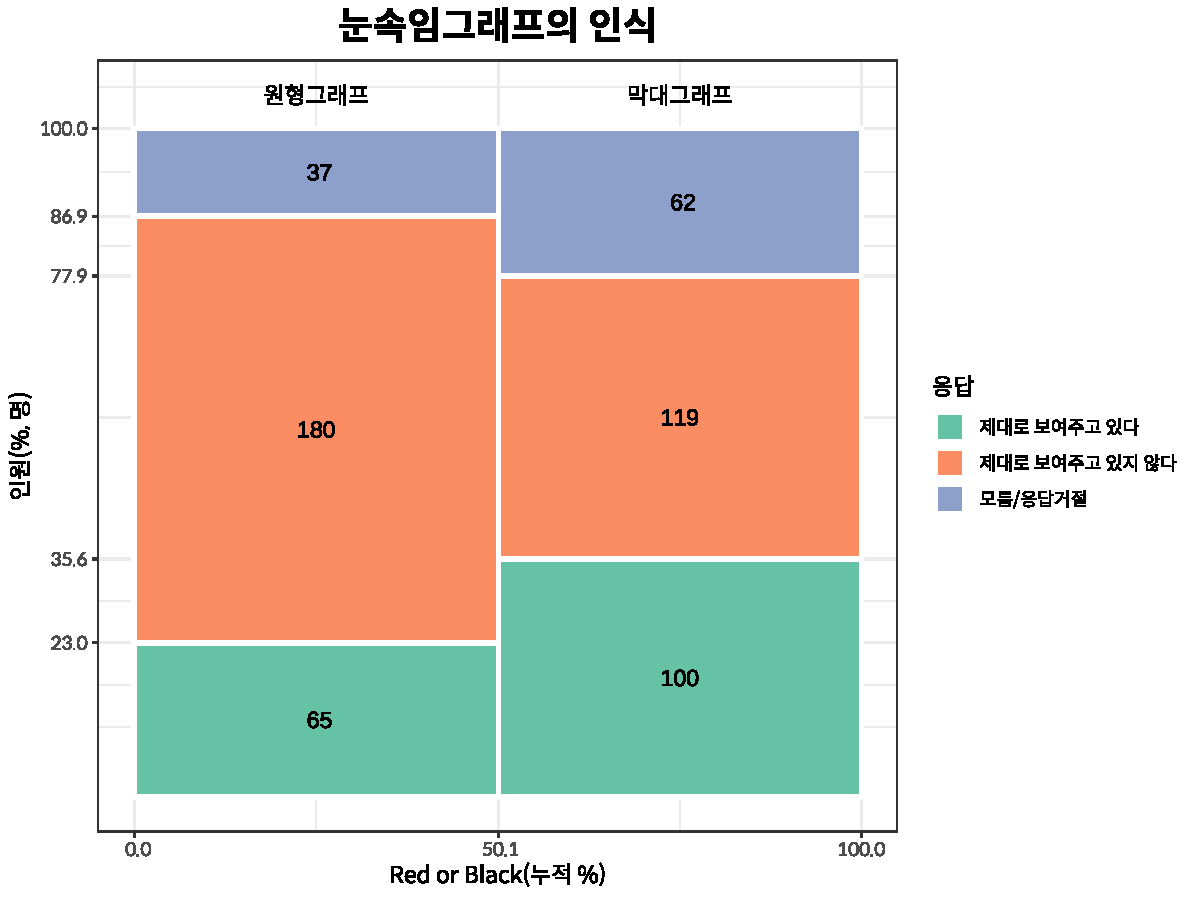
\includegraphics{_main_files/figure-latex/unnamed-chunk-49-1.pdf}

Mosaic Plot 은 이 집계결과를 시각적으로 잘 보여줍니다.

원형그래프의 각도를 왜곡한 Red 에서 여론조사 결과를 ``제대로 보여주고 있다''고 응답한 백분율이 매우 낮고, 막대그래프의 높이를 왜곡한 Black 에서 여론조사 결과를 ``제대로 보여주고 있다''고 응답한 백분율은 상대적으로 덜 낮은 것을 시각적으로 알 수 있습니다.

\section{마감 시간으로부터 제출 시간의 분포}\label{uxb9c8uxac10-uxc2dcuxac04uxc73cuxb85cuxbd80uxd130-uxc81cuxcd9c-uxc2dcuxac04uxc758-uxbd84uxd3ec-1}

\subsection{분포표}\label{uxbd84uxd3ecuxd45c-2}

\begin{longtable}[]{@{}
  >{\raggedright\arraybackslash}p{(\columnwidth - 30\tabcolsep) * \real{0.0863}}
  >{\raggedleft\arraybackslash}p{(\columnwidth - 30\tabcolsep) * \real{0.0576}}
  >{\raggedleft\arraybackslash}p{(\columnwidth - 30\tabcolsep) * \real{0.0576}}
  >{\raggedleft\arraybackslash}p{(\columnwidth - 30\tabcolsep) * \real{0.0576}}
  >{\raggedleft\arraybackslash}p{(\columnwidth - 30\tabcolsep) * \real{0.0576}}
  >{\raggedleft\arraybackslash}p{(\columnwidth - 30\tabcolsep) * \real{0.0576}}
  >{\raggedleft\arraybackslash}p{(\columnwidth - 30\tabcolsep) * \real{0.0576}}
  >{\raggedleft\arraybackslash}p{(\columnwidth - 30\tabcolsep) * \real{0.0576}}
  >{\raggedleft\arraybackslash}p{(\columnwidth - 30\tabcolsep) * \real{0.0576}}
  >{\raggedleft\arraybackslash}p{(\columnwidth - 30\tabcolsep) * \real{0.0576}}
  >{\raggedleft\arraybackslash}p{(\columnwidth - 30\tabcolsep) * \real{0.0647}}
  >{\raggedleft\arraybackslash}p{(\columnwidth - 30\tabcolsep) * \real{0.0719}}
  >{\raggedleft\arraybackslash}p{(\columnwidth - 30\tabcolsep) * \real{0.0719}}
  >{\raggedleft\arraybackslash}p{(\columnwidth - 30\tabcolsep) * \real{0.0719}}
  >{\raggedleft\arraybackslash}p{(\columnwidth - 30\tabcolsep) * \real{0.0719}}
  >{\centering\arraybackslash}p{(\columnwidth - 30\tabcolsep) * \real{0.0432}}@{}}
\caption{일 단위}\tabularnewline
\toprule\noalign{}
\begin{minipage}[b]{\linewidth}\raggedright
~
\end{minipage} & \begin{minipage}[b]{\linewidth}\raggedleft
{[}0,1{]}
\end{minipage} & \begin{minipage}[b]{\linewidth}\raggedleft
(1,2{]}
\end{minipage} & \begin{minipage}[b]{\linewidth}\raggedleft
(2,3{]}
\end{minipage} & \begin{minipage}[b]{\linewidth}\raggedleft
(3,4{]}
\end{minipage} & \begin{minipage}[b]{\linewidth}\raggedleft
(4,5{]}
\end{minipage} & \begin{minipage}[b]{\linewidth}\raggedleft
(5,6{]}
\end{minipage} & \begin{minipage}[b]{\linewidth}\raggedleft
(6,7{]}
\end{minipage} & \begin{minipage}[b]{\linewidth}\raggedleft
(7,8{]}
\end{minipage} & \begin{minipage}[b]{\linewidth}\raggedleft
(8,9{]}
\end{minipage} & \begin{minipage}[b]{\linewidth}\raggedleft
(9,10{]}
\end{minipage} & \begin{minipage}[b]{\linewidth}\raggedleft
(10,11{]}
\end{minipage} & \begin{minipage}[b]{\linewidth}\raggedleft
(11,12{]}
\end{minipage} & \begin{minipage}[b]{\linewidth}\raggedleft
(12,13{]}
\end{minipage} & \begin{minipage}[b]{\linewidth}\raggedleft
(13,14{]}
\end{minipage} & \begin{minipage}[b]{\linewidth}\centering
계
\end{minipage} \\
\midrule\noalign{}
\endfirsthead
\toprule\noalign{}
\begin{minipage}[b]{\linewidth}\raggedright
~
\end{minipage} & \begin{minipage}[b]{\linewidth}\raggedleft
{[}0,1{]}
\end{minipage} & \begin{minipage}[b]{\linewidth}\raggedleft
(1,2{]}
\end{minipage} & \begin{minipage}[b]{\linewidth}\raggedleft
(2,3{]}
\end{minipage} & \begin{minipage}[b]{\linewidth}\raggedleft
(3,4{]}
\end{minipage} & \begin{minipage}[b]{\linewidth}\raggedleft
(4,5{]}
\end{minipage} & \begin{minipage}[b]{\linewidth}\raggedleft
(5,6{]}
\end{minipage} & \begin{minipage}[b]{\linewidth}\raggedleft
(6,7{]}
\end{minipage} & \begin{minipage}[b]{\linewidth}\raggedleft
(7,8{]}
\end{minipage} & \begin{minipage}[b]{\linewidth}\raggedleft
(8,9{]}
\end{minipage} & \begin{minipage}[b]{\linewidth}\raggedleft
(9,10{]}
\end{minipage} & \begin{minipage}[b]{\linewidth}\raggedleft
(10,11{]}
\end{minipage} & \begin{minipage}[b]{\linewidth}\raggedleft
(11,12{]}
\end{minipage} & \begin{minipage}[b]{\linewidth}\raggedleft
(12,13{]}
\end{minipage} & \begin{minipage}[b]{\linewidth}\raggedleft
(13,14{]}
\end{minipage} & \begin{minipage}[b]{\linewidth}\centering
계
\end{minipage} \\
\midrule\noalign{}
\endhead
\bottomrule\noalign{}
\endlastfoot
\textbf{Red} & 52 & 17 & 9 & 6 & 12 & 8 & 12 & 51 & 20 & 13 & 21 & 13 & 21 & 27 & 282 \\
\textbf{Black} & 59 & 11 & 11 & 3 & 6 & 7 & 9 & 43 & 19 & 18 & 20 & 21 & 26 & 28 & 281 \\
\textbf{계} & 111 & 28 & 20 & 9 & 18 & 15 & 21 & 94 & 39 & 31 & 41 & 34 & 47 & 55 & 563 \\
\end{longtable}

분포표로부터 두 가지 문제를 살펴보겠습니다.

첫째, 날마다 고르게 제출하는가?

둘째, Red, Black 간에 통계적으로 유의한 차이가 있는가?

각 문제를 살펴보기 위해서는 분포표의 일부분을 대상으로 카이제곱 테스트를 수행합니다.

\subsection{날마다 고르게 제출하는가?}\label{uxb0a0uxb9c8uxb2e4-uxace0uxb974uxac8c-uxc81cuxcd9cuxd558uxb294uxac00-1}

\begin{longtable}[]{@{}
  >{\raggedleft\arraybackslash}p{(\columnwidth - 24\tabcolsep) * \real{0.0708}}
  >{\raggedleft\arraybackslash}p{(\columnwidth - 24\tabcolsep) * \real{0.0708}}
  >{\raggedleft\arraybackslash}p{(\columnwidth - 24\tabcolsep) * \real{0.0708}}
  >{\raggedleft\arraybackslash}p{(\columnwidth - 24\tabcolsep) * \real{0.0708}}
  >{\raggedleft\arraybackslash}p{(\columnwidth - 24\tabcolsep) * \real{0.0708}}
  >{\raggedleft\arraybackslash}p{(\columnwidth - 24\tabcolsep) * \real{0.0708}}
  >{\raggedleft\arraybackslash}p{(\columnwidth - 24\tabcolsep) * \real{0.0708}}
  >{\raggedleft\arraybackslash}p{(\columnwidth - 24\tabcolsep) * \real{0.0708}}
  >{\raggedleft\arraybackslash}p{(\columnwidth - 24\tabcolsep) * \real{0.0796}}
  >{\raggedleft\arraybackslash}p{(\columnwidth - 24\tabcolsep) * \real{0.0885}}
  >{\raggedleft\arraybackslash}p{(\columnwidth - 24\tabcolsep) * \real{0.0885}}
  >{\raggedleft\arraybackslash}p{(\columnwidth - 24\tabcolsep) * \real{0.0885}}
  >{\raggedleft\arraybackslash}p{(\columnwidth - 24\tabcolsep) * \real{0.0885}}@{}}
\toprule\noalign{}
\begin{minipage}[b]{\linewidth}\raggedleft
(1,2{]}
\end{minipage} & \begin{minipage}[b]{\linewidth}\raggedleft
(2,3{]}
\end{minipage} & \begin{minipage}[b]{\linewidth}\raggedleft
(3,4{]}
\end{minipage} & \begin{minipage}[b]{\linewidth}\raggedleft
(4,5{]}
\end{minipage} & \begin{minipage}[b]{\linewidth}\raggedleft
(5,6{]}
\end{minipage} & \begin{minipage}[b]{\linewidth}\raggedleft
(6,7{]}
\end{minipage} & \begin{minipage}[b]{\linewidth}\raggedleft
(7,8{]}
\end{minipage} & \begin{minipage}[b]{\linewidth}\raggedleft
(8,9{]}
\end{minipage} & \begin{minipage}[b]{\linewidth}\raggedleft
(9,10{]}
\end{minipage} & \begin{minipage}[b]{\linewidth}\raggedleft
(10,11{]}
\end{minipage} & \begin{minipage}[b]{\linewidth}\raggedleft
(11,12{]}
\end{minipage} & \begin{minipage}[b]{\linewidth}\raggedleft
(12,13{]}
\end{minipage} & \begin{minipage}[b]{\linewidth}\raggedleft
(13,14{]}
\end{minipage} \\
\midrule\noalign{}
\endhead
\bottomrule\noalign{}
\endlastfoot
28 & 20 & 9 & 18 & 15 & 21 & 94 & 39 & 31 & 41 & 34 & 47 & 55 \\
\end{longtable}

\begin{longtable}[]{@{}
  >{\raggedleft\arraybackslash}p{(\columnwidth - 4\tabcolsep) * \real{0.2361}}
  >{\raggedleft\arraybackslash}p{(\columnwidth - 4\tabcolsep) * \real{0.0694}}
  >{\raggedleft\arraybackslash}p{(\columnwidth - 4\tabcolsep) * \real{0.2500}}@{}}
\caption{Chi-squared test for given probabilities: \texttt{.}}\tabularnewline
\toprule\noalign{}
\begin{minipage}[b]{\linewidth}\raggedleft
Test statistic
\end{minipage} & \begin{minipage}[b]{\linewidth}\raggedleft
df
\end{minipage} & \begin{minipage}[b]{\linewidth}\raggedleft
P value
\end{minipage} \\
\midrule\noalign{}
\endfirsthead
\toprule\noalign{}
\begin{minipage}[b]{\linewidth}\raggedleft
Test statistic
\end{minipage} & \begin{minipage}[b]{\linewidth}\raggedleft
df
\end{minipage} & \begin{minipage}[b]{\linewidth}\raggedleft
P value
\end{minipage} \\
\midrule\noalign{}
\endhead
\bottomrule\noalign{}
\endlastfoot
170.5 & 12 & 3.764e-30 * * * \\
\end{longtable}

날마다 고르게 제출하는지 알아 보았습니다.

분포표의 ``계''행에서 '계'열을 제외하고 카이제곱테스트를 수행합니다.

분포표 만으로도 쉽게 파악할 수 있지만 카이제곱테스트가 명확히 해 줍니다.

카이제곱 통계량은 170.50, 자유도는 12.00, p-value 는 3.8e-30 이므로 결코 고르게 제출한다고 말할 수 없겠습니다.

막대그래프로 살펴 보겠습니다.

\subsection{막대그래프}\label{uxb9c9uxb300uxadf8uxb798uxd504-2}

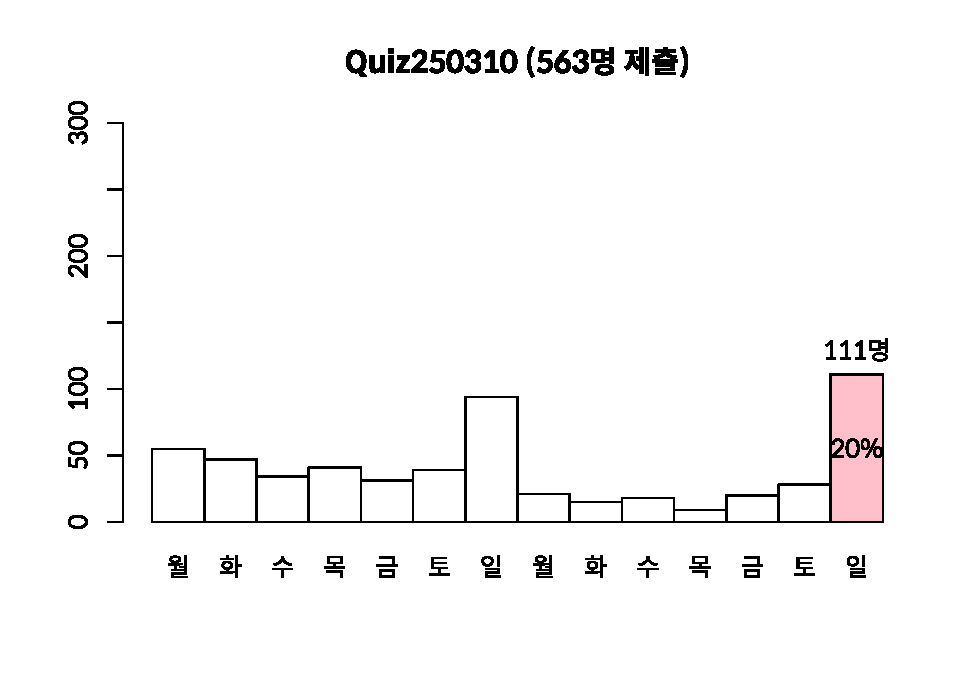
\includegraphics{_main_files/figure-latex/unnamed-chunk-52-1.pdf}

막대그래프는 총 제출인원 563(명) 중에 111(명), 20(\%)가 마감일에 몰리는 것을 명확히 보여주고 있습니다.

\subsection{Red, Black 간에 닮았는가?}\label{red-black-uxac04uxc5d0-uxb2eeuxc558uxb294uxac00-1}

\begin{longtable}[]{@{}
  >{\raggedright\arraybackslash}p{(\columnwidth - 26\tabcolsep) * \real{0.0960}}
  >{\raggedleft\arraybackslash}p{(\columnwidth - 26\tabcolsep) * \real{0.0640}}
  >{\raggedleft\arraybackslash}p{(\columnwidth - 26\tabcolsep) * \real{0.0640}}
  >{\raggedleft\arraybackslash}p{(\columnwidth - 26\tabcolsep) * \real{0.0640}}
  >{\raggedleft\arraybackslash}p{(\columnwidth - 26\tabcolsep) * \real{0.0640}}
  >{\raggedleft\arraybackslash}p{(\columnwidth - 26\tabcolsep) * \real{0.0640}}
  >{\raggedleft\arraybackslash}p{(\columnwidth - 26\tabcolsep) * \real{0.0640}}
  >{\raggedleft\arraybackslash}p{(\columnwidth - 26\tabcolsep) * \real{0.0640}}
  >{\raggedleft\arraybackslash}p{(\columnwidth - 26\tabcolsep) * \real{0.0640}}
  >{\raggedleft\arraybackslash}p{(\columnwidth - 26\tabcolsep) * \real{0.0720}}
  >{\raggedleft\arraybackslash}p{(\columnwidth - 26\tabcolsep) * \real{0.0800}}
  >{\raggedleft\arraybackslash}p{(\columnwidth - 26\tabcolsep) * \real{0.0800}}
  >{\raggedleft\arraybackslash}p{(\columnwidth - 26\tabcolsep) * \real{0.0800}}
  >{\raggedleft\arraybackslash}p{(\columnwidth - 26\tabcolsep) * \real{0.0800}}@{}}
\toprule\noalign{}
\begin{minipage}[b]{\linewidth}\raggedright
~
\end{minipage} & \begin{minipage}[b]{\linewidth}\raggedleft
(1,2{]}
\end{minipage} & \begin{minipage}[b]{\linewidth}\raggedleft
(2,3{]}
\end{minipage} & \begin{minipage}[b]{\linewidth}\raggedleft
(3,4{]}
\end{minipage} & \begin{minipage}[b]{\linewidth}\raggedleft
(4,5{]}
\end{minipage} & \begin{minipage}[b]{\linewidth}\raggedleft
(5,6{]}
\end{minipage} & \begin{minipage}[b]{\linewidth}\raggedleft
(6,7{]}
\end{minipage} & \begin{minipage}[b]{\linewidth}\raggedleft
(7,8{]}
\end{minipage} & \begin{minipage}[b]{\linewidth}\raggedleft
(8,9{]}
\end{minipage} & \begin{minipage}[b]{\linewidth}\raggedleft
(9,10{]}
\end{minipage} & \begin{minipage}[b]{\linewidth}\raggedleft
(10,11{]}
\end{minipage} & \begin{minipage}[b]{\linewidth}\raggedleft
(11,12{]}
\end{minipage} & \begin{minipage}[b]{\linewidth}\raggedleft
(12,13{]}
\end{minipage} & \begin{minipage}[b]{\linewidth}\raggedleft
(13,14{]}
\end{minipage} \\
\midrule\noalign{}
\endhead
\bottomrule\noalign{}
\endlastfoot
\textbf{Red} & 17 & 9 & 6 & 12 & 8 & 12 & 51 & 20 & 13 & 21 & 13 & 21 & 27 \\
\textbf{Black} & 11 & 11 & 3 & 6 & 7 & 9 & 43 & 19 & 18 & 20 & 21 & 26 & 28 \\
\end{longtable}

\begin{longtable}[]{@{}
  >{\raggedleft\arraybackslash}p{(\columnwidth - 4\tabcolsep) * \real{0.2361}}
  >{\raggedleft\arraybackslash}p{(\columnwidth - 4\tabcolsep) * \real{0.0694}}
  >{\raggedleft\arraybackslash}p{(\columnwidth - 4\tabcolsep) * \real{0.1389}}@{}}
\caption{Pearson's Chi-squared test: \texttt{.}}\tabularnewline
\toprule\noalign{}
\begin{minipage}[b]{\linewidth}\raggedleft
Test statistic
\end{minipage} & \begin{minipage}[b]{\linewidth}\raggedleft
df
\end{minipage} & \begin{minipage}[b]{\linewidth}\raggedleft
P value
\end{minipage} \\
\midrule\noalign{}
\endfirsthead
\toprule\noalign{}
\begin{minipage}[b]{\linewidth}\raggedleft
Test statistic
\end{minipage} & \begin{minipage}[b]{\linewidth}\raggedleft
df
\end{minipage} & \begin{minipage}[b]{\linewidth}\raggedleft
P value
\end{minipage} \\
\midrule\noalign{}
\endhead
\bottomrule\noalign{}
\endlastfoot
8.812 & 12 & 0.7189 \\
\end{longtable}

제출시간의 분포가 Red, Black 간에 닮았는지 알아 보았습니다.

이번에는 분포표의 첫번째와 두번째 행, '계'열을 제외한 나머지 열에 대해서 카이제곱테스트를 수행합니다.

카이제곱 통계량은 8.812, 자유도는 12, p-value 는 0.7189 이므로 제출 시간의 분포는 Red, Black 간에 통계적으로 유의한 차이가 관찰되지 않습니다.

이 사실을 Mosaic Plot 을 이용하여 시각적으로 살펴보겠습니다.

닮았다고 느껴지나요?

\subsection{Mosaic Plot}\label{mosaic-plot-3}

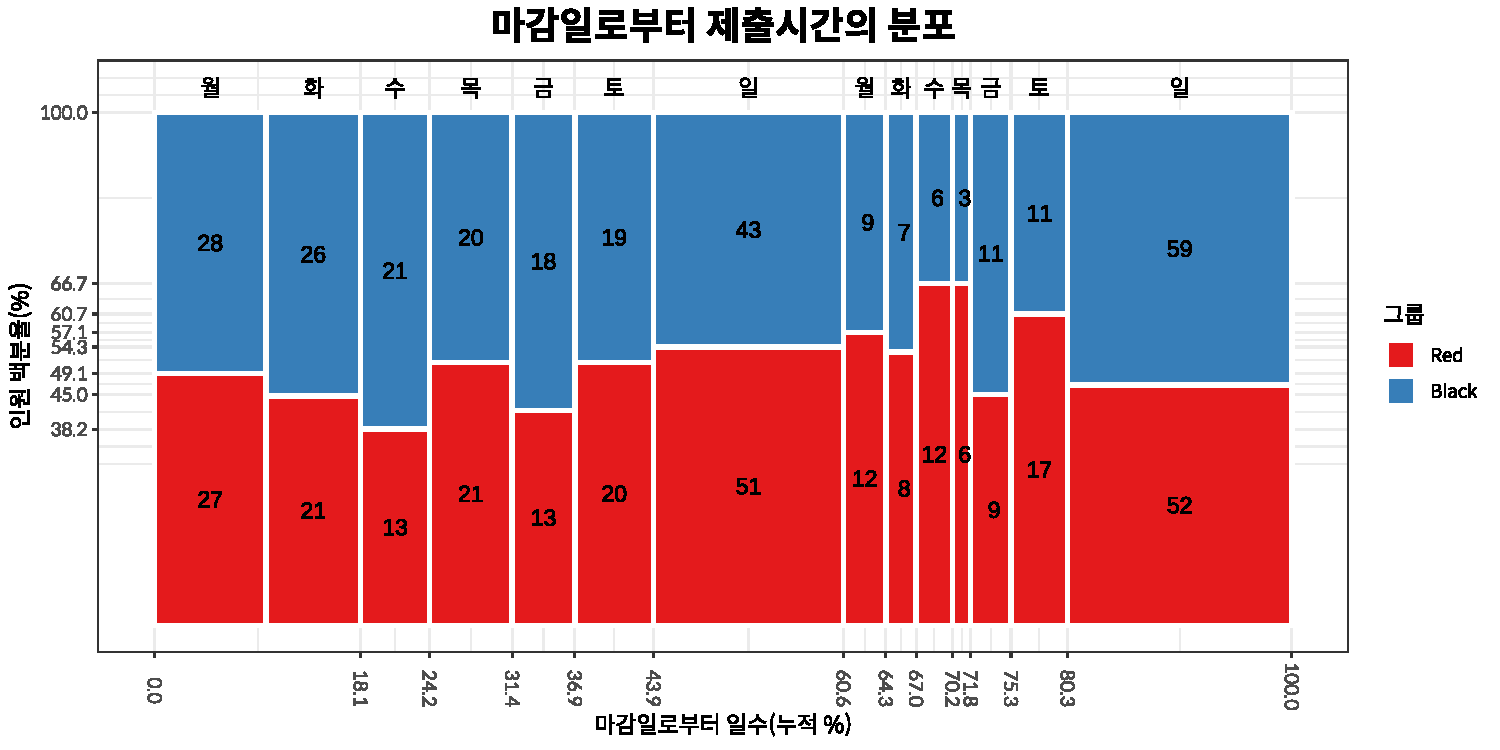
\includegraphics{_main_files/figure-latex/unnamed-chunk-54-1.pdf}

\chapter{3주차 데이터 실험 집계}\label{uxc8fcuxcc28-uxb370uxc774uxd130-uxc2e4uxd5d8-uxc9d1uxacc4-2}

\section{실험의 목적}\label{uxc2e4uxd5d8uxc758-uxbaa9uxc801-2}

3주차 구글 예습 설문지 집계결과를 분석합니다.

Q1\textasciitilde Q6에서는 랜덤화의 효과로 Red, Black 이 얼마나 닮았는지 알아봅니다.

Q7에서는 같은 사안에 대해서 질문 안에 편향된 정보를 담아 넣었을 때 Red, Black 의 응답이 어떻게 달라지는 지 알아봅니다.

끝으로 제출시간의 분포가 날마다 고른지, Red, Black 간에는 닮았는지 알아봅니다.

\subsection{Red, Black을 잘못 표시한 사람들}\label{red-blackuxc744-uxc798uxbabb-uxd45cuxc2dcuxd55c-uxc0acuxb78cuxb4e4-2}

\begin{longtable}[]{@{}
  >{\raggedright\arraybackslash}p{(\columnwidth - 4\tabcolsep) * \real{0.3611}}
  >{\centering\arraybackslash}p{(\columnwidth - 4\tabcolsep) * \real{0.2778}}
  >{\centering\arraybackslash}p{(\columnwidth - 4\tabcolsep) * \real{0.3056}}@{}}
\toprule\noalign{}
\begin{minipage}[b]{\linewidth}\raggedright
~
\end{minipage} & \begin{minipage}[b]{\linewidth}\centering
Red(구글예습퀴즈)
\end{minipage} & \begin{minipage}[b]{\linewidth}\centering
Black(구글예습퀴즈)
\end{minipage} \\
\midrule\noalign{}
\endhead
\bottomrule\noalign{}
\endlastfoot
\textbf{Red(랜덤화출석부)} & 273 & 5 \\
\textbf{Black(랜덤화출석부)} & 4 & 271 \\
\textbf{계} & 277 & 276 \\
\end{longtable}

랜덤화출석부에 있는 Red, Black 과 실제 구글설문에 올린 Red, Black 이 다른 사람들의 수효는 9명입니다.

Red를 Black 이라고 한 사람이 5명, Black 을 Red 라고 한 사람이 4명입니다.

두 가지 방법으로 분석합니다.

우선 Red, Black 을 잘못 선택한 9명을 랜덤하게 둘로 나누면 어느 한 쪽 집단에 들어갈 기대인원은 9명을 둘로 나눈 4.5(명)이고, 표준오차는 9의 제곱근에 1/2을 곱해 준 1.5명이 됩니다.

실제로 Red를 Black 이라고 한 사람수, 5명이나 Black 을 Red 라고 한 사람수, 4명은 기대인원으로부터 표준오차 범위 안에 아주 잘 들어갑니다.

두 번째 분석 방법은 확률을 계산해 보는 것입니다.

Red, Black 을 잘못 선택한 9명을 랜덤하게 둘로 나눌 때, 실제로 관찰된 5명 이상이나 4명이하로 잘못 선택한 사람수가 나올 가능성은 얼마나 되는가 입니다.

이 경우 공평한 동전던지기를 확률 법칙으로 표현한 이항분포로부터 계산할 수 있습니다.

시행횟수가 9이고 한 번 시행에서 성공확률이 1/2 인 이항분포에서 성공횟수가 4이하이거나 5이상을 관찰할 확률은 1입니다.

공평한 동전 던지기에서 앞면이 4개 이하 나오는 확률은 5개 이상 나오는 확률과 같기 때문에 사실상 한쪽만 계산해서 2배 해 주면 됩니다.

이 값을 p-value 라고 하는데, p-value가 0.05보다 작을 때 \textbf{통계적으로 유의한 차이를 관찰}하였다고 말합니다.

즉, 공평한 동전을 던지는 것과 같은 과정이라고 가정하였을 때 실제로 관찰된 값들이 가정으로부터 얼마나 떨어져 있는지를 표현한 것입니다.

0.05, 즉 1/20은 이런 실험을 스무 번 정도 반복하면 1번 나올 정도로 드문 사건을 의미합니다.

즉 가정이 타당하다면 나오기 힘든 결과라는 것입니다.

그런데 Red, Black 을 잘못 표시한 사람들의 분포에서 관찰된 p-value 는 0.05와는 비교도 안될 정도로 큰 값입니다.

따라서 두 집단이 랜덤화 효과가 작동하여 \textbf{통계적으로 유의한 차이를 보이지 않는다}고 할 수 있습니다.

\subsection{응답인원의 Red, Black}\label{uxc751uxb2f5uxc778uxc6d0uxc758-red-black-2}

Red 로 응답한 인원은 277명, Black 에 응답한 인원은 276명입니다.

전체 응답인원 553 명을 랜덤하게 둘로 나눌 때 어느 한 쪽의 기대인원은 전체 응답인원의 절반인 276.5명이고, 표준오차는 전체 응답인원의 제곱근에 1/2을 곱해 준 11.8 명입니다.

따라서 Red, Black 각 그룹에 관찰된 인원은 기대인원으로부터 표준오차 범위 안에 들어갑니다.

\section{Q1. 국세와 지방세 비중}\label{q1.-uxad6duxc138uxc640-uxc9c0uxbc29uxc138-uxbe44uxc911}

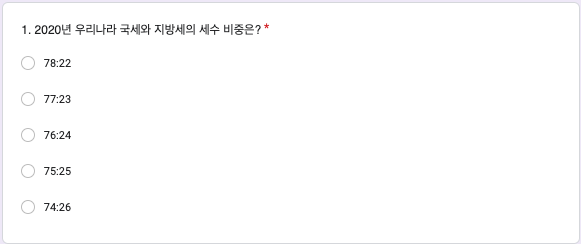
\includegraphics[width=0.75\linewidth]{./pics/Quiz230315_Q1}

\subsection{국세와 지방세 비중(집계표)}\label{uxad6duxc138uxc640-uxc9c0uxbc29uxc138-uxbe44uxc911uxc9d1uxacc4uxd45c}

\begin{longtable}[]{@{}
  >{\raggedright\arraybackslash}p{(\columnwidth - 12\tabcolsep) * \real{0.1667}}
  >{\raggedleft\arraybackslash}p{(\columnwidth - 12\tabcolsep) * \real{0.1111}}
  >{\raggedleft\arraybackslash}p{(\columnwidth - 12\tabcolsep) * \real{0.1111}}
  >{\raggedleft\arraybackslash}p{(\columnwidth - 12\tabcolsep) * \real{0.1111}}
  >{\raggedleft\arraybackslash}p{(\columnwidth - 12\tabcolsep) * \real{0.1111}}
  >{\raggedleft\arraybackslash}p{(\columnwidth - 12\tabcolsep) * \real{0.1111}}
  >{\centering\arraybackslash}p{(\columnwidth - 12\tabcolsep) * \real{0.1111}}@{}}
\toprule\noalign{}
\begin{minipage}[b]{\linewidth}\raggedright
~
\end{minipage} & \begin{minipage}[b]{\linewidth}\raggedleft
78:22
\end{minipage} & \begin{minipage}[b]{\linewidth}\raggedleft
77:23
\end{minipage} & \begin{minipage}[b]{\linewidth}\raggedleft
76:24
\end{minipage} & \begin{minipage}[b]{\linewidth}\raggedleft
75:25
\end{minipage} & \begin{minipage}[b]{\linewidth}\raggedleft
74:26
\end{minipage} & \begin{minipage}[b]{\linewidth}\centering
계
\end{minipage} \\
\midrule\noalign{}
\endhead
\bottomrule\noalign{}
\endlastfoot
\textbf{Red} & 16 & 35 & 45 & 29 & 152 & 277 \\
\textbf{Black} & 16 & 33 & 55 & 23 & 149 & 276 \\
\textbf{계} & 32 & 68 & 100 & 52 & 301 & 553 \\
\end{longtable}

\begin{longtable}[]{@{}
  >{\raggedleft\arraybackslash}p{(\columnwidth - 4\tabcolsep) * \real{0.2361}}
  >{\raggedleft\arraybackslash}p{(\columnwidth - 4\tabcolsep) * \real{0.0694}}
  >{\raggedleft\arraybackslash}p{(\columnwidth - 4\tabcolsep) * \real{0.1389}}@{}}
\caption{Pearson's Chi-squared test: \texttt{.}}\tabularnewline
\toprule\noalign{}
\begin{minipage}[b]{\linewidth}\raggedleft
Test statistic
\end{minipage} & \begin{minipage}[b]{\linewidth}\raggedleft
df
\end{minipage} & \begin{minipage}[b]{\linewidth}\raggedleft
P value
\end{minipage} \\
\midrule\noalign{}
\endfirsthead
\toprule\noalign{}
\begin{minipage}[b]{\linewidth}\raggedleft
Test statistic
\end{minipage} & \begin{minipage}[b]{\linewidth}\raggedleft
df
\end{minipage} & \begin{minipage}[b]{\linewidth}\raggedleft
P value
\end{minipage} \\
\midrule\noalign{}
\endhead
\bottomrule\noalign{}
\endlastfoot
1.779 & 4 & 0.7763 \\
\end{longtable}

Q1의 집계 결과가 Red, Black 간에 통계적으로 유의한 차이가 있는지 알아보기 위하여 카이제곱 테스트를 수행하였습니다.

그 결과 카이제곱 통계량은 1.78, 자유도는 4 , p-value 는 0.7763이므로 Red, Black 간에 통계적으로 유의한 차이를 보이지 않습니다.

실제로 닮은 게 느껴집니까?

\subsection{국세와 지방세 비중(\%)}\label{uxad6duxc138uxc640-uxc9c0uxbc29uxc138-uxbe44uxc911}

\begin{longtable}[]{@{}
  >{\raggedleft\arraybackslash}p{(\columnwidth - 10\tabcolsep) * \real{0.1111}}
  >{\raggedleft\arraybackslash}p{(\columnwidth - 10\tabcolsep) * \real{0.1111}}
  >{\raggedleft\arraybackslash}p{(\columnwidth - 10\tabcolsep) * \real{0.1111}}
  >{\raggedleft\arraybackslash}p{(\columnwidth - 10\tabcolsep) * \real{0.1111}}
  >{\raggedleft\arraybackslash}p{(\columnwidth - 10\tabcolsep) * \real{0.1111}}
  >{\centering\arraybackslash}p{(\columnwidth - 10\tabcolsep) * \real{0.1111}}@{}}
\toprule\noalign{}
\begin{minipage}[b]{\linewidth}\raggedleft
78:22
\end{minipage} & \begin{minipage}[b]{\linewidth}\raggedleft
77:23
\end{minipage} & \begin{minipage}[b]{\linewidth}\raggedleft
76:24
\end{minipage} & \begin{minipage}[b]{\linewidth}\raggedleft
75:25
\end{minipage} & \begin{minipage}[b]{\linewidth}\raggedleft
74:26
\end{minipage} & \begin{minipage}[b]{\linewidth}\centering
계
\end{minipage} \\
\midrule\noalign{}
\endhead
\bottomrule\noalign{}
\endlastfoot
5.8 & 12.3 & 18.1 & 9.4 & 54.4 & 100.0 \\
\end{longtable}

정답률은 Red, Black 을 합하여 계산하는데, 54.4(\%) 입니다.

\section{Q2. 조세부담률}\label{q2.-uxc870uxc138uxbd80uxb2f4uxb960}


\includegraphics[width=0.75\linewidth]{./pics/Quiz230315_Q2}

\subsection{조세부담률(집계표)}\label{uxc870uxc138uxbd80uxb2f4uxb960uxc9d1uxacc4uxd45c}

\begin{longtable}[]{@{}
  >{\raggedright\arraybackslash}p{(\columnwidth - 12\tabcolsep) * \real{0.1667}}
  >{\raggedleft\arraybackslash}p{(\columnwidth - 12\tabcolsep) * \real{0.0833}}
  >{\raggedleft\arraybackslash}p{(\columnwidth - 12\tabcolsep) * \real{0.0833}}
  >{\raggedleft\arraybackslash}p{(\columnwidth - 12\tabcolsep) * \real{0.0833}}
  >{\raggedleft\arraybackslash}p{(\columnwidth - 12\tabcolsep) * \real{0.0833}}
  >{\raggedleft\arraybackslash}p{(\columnwidth - 12\tabcolsep) * \real{0.0833}}
  >{\centering\arraybackslash}p{(\columnwidth - 12\tabcolsep) * \real{0.0833}}@{}}
\toprule\noalign{}
\begin{minipage}[b]{\linewidth}\raggedright
~
\end{minipage} & \begin{minipage}[b]{\linewidth}\raggedleft
10\%
\end{minipage} & \begin{minipage}[b]{\linewidth}\raggedleft
15\%
\end{minipage} & \begin{minipage}[b]{\linewidth}\raggedleft
20\%
\end{minipage} & \begin{minipage}[b]{\linewidth}\raggedleft
25\%
\end{minipage} & \begin{minipage}[b]{\linewidth}\raggedleft
30\%
\end{minipage} & \begin{minipage}[b]{\linewidth}\centering
계
\end{minipage} \\
\midrule\noalign{}
\endhead
\bottomrule\noalign{}
\endlastfoot
\textbf{Red} & 6 & 28 & 223 & 17 & 3 & 277 \\
\textbf{Black} & 7 & 24 & 221 & 19 & 5 & 276 \\
\textbf{계} & 13 & 52 & 444 & 36 & 8 & 553 \\
\end{longtable}

\begin{longtable}[]{@{}
  >{\raggedleft\arraybackslash}p{(\columnwidth - 4\tabcolsep) * \real{0.2361}}
  >{\raggedleft\arraybackslash}p{(\columnwidth - 4\tabcolsep) * \real{0.0694}}
  >{\raggedleft\arraybackslash}p{(\columnwidth - 4\tabcolsep) * \real{0.1389}}@{}}
\caption{Pearson's Chi-squared test: \texttt{.}}\tabularnewline
\toprule\noalign{}
\begin{minipage}[b]{\linewidth}\raggedleft
Test statistic
\end{minipage} & \begin{minipage}[b]{\linewidth}\raggedleft
df
\end{minipage} & \begin{minipage}[b]{\linewidth}\raggedleft
P value
\end{minipage} \\
\midrule\noalign{}
\endfirsthead
\toprule\noalign{}
\begin{minipage}[b]{\linewidth}\raggedleft
Test statistic
\end{minipage} & \begin{minipage}[b]{\linewidth}\raggedleft
df
\end{minipage} & \begin{minipage}[b]{\linewidth}\raggedleft
P value
\end{minipage} \\
\midrule\noalign{}
\endhead
\bottomrule\noalign{}
\endlastfoot
1.003 & 4 & 0.9094 \\
\end{longtable}

Q2의 집계 결과가 Red, Black 간에 통계적으로 유의한 차이가 있는지 알아보기 위하여 카이제곱 테스트를 수행하였습니다.

그 결과 카이제곱 통계량은 1.003, 자유도는 4, p-value 는 0.9094이므로 Red, Black 간에 통계적으로 유의한 차이를 보이지 않습니다.

실제로 닮은 게 느껴집니까?

\subsection{조세부담률(\%)}\label{uxc870uxc138uxbd80uxb2f4uxb960}

\begin{longtable}[]{@{}
  >{\raggedleft\arraybackslash}p{(\columnwidth - 10\tabcolsep) * \real{0.0833}}
  >{\raggedleft\arraybackslash}p{(\columnwidth - 10\tabcolsep) * \real{0.0833}}
  >{\raggedleft\arraybackslash}p{(\columnwidth - 10\tabcolsep) * \real{0.0972}}
  >{\raggedleft\arraybackslash}p{(\columnwidth - 10\tabcolsep) * \real{0.0833}}
  >{\raggedleft\arraybackslash}p{(\columnwidth - 10\tabcolsep) * \real{0.0833}}
  >{\centering\arraybackslash}p{(\columnwidth - 10\tabcolsep) * \real{0.1111}}@{}}
\toprule\noalign{}
\begin{minipage}[b]{\linewidth}\raggedleft
10\%
\end{minipage} & \begin{minipage}[b]{\linewidth}\raggedleft
15\%
\end{minipage} & \begin{minipage}[b]{\linewidth}\raggedleft
20\%
\end{minipage} & \begin{minipage}[b]{\linewidth}\raggedleft
25\%
\end{minipage} & \begin{minipage}[b]{\linewidth}\raggedleft
30\%
\end{minipage} & \begin{minipage}[b]{\linewidth}\centering
계
\end{minipage} \\
\midrule\noalign{}
\endhead
\bottomrule\noalign{}
\endlastfoot
2.4 & 9.4 & 80.3 & 6.5 & 1.4 & 100.0 \\
\end{longtable}

정답률은 Red, Black 을 합하여 계산하는데, 80.3(\%) 입니다.

\section{Q3. OECD 국민부담률}\label{q3.-oecd-uxad6duxbbfcuxbd80uxb2f4uxb960}

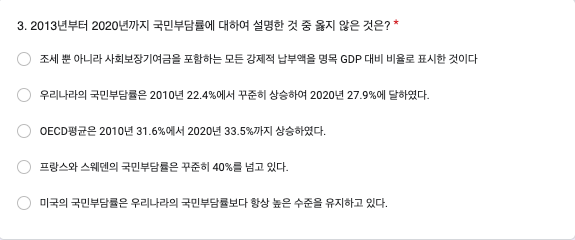
\includegraphics[width=0.75\linewidth]{./pics/Quiz230315_Q3}

\subsection{OECD 국민부담률(집계표)}\label{oecd-uxad6duxbbfcuxbd80uxb2f4uxb960uxc9d1uxacc4uxd45c}

\begin{longtable}[]{@{}
  >{\raggedright\arraybackslash}p{(\columnwidth - 12\tabcolsep) * \real{0.0663}}
  >{\centering\arraybackslash}p{(\columnwidth - 12\tabcolsep) * \real{0.1823}}
  >{\centering\arraybackslash}p{(\columnwidth - 12\tabcolsep) * \real{0.1823}}
  >{\centering\arraybackslash}p{(\columnwidth - 12\tabcolsep) * \real{0.1713}}
  >{\centering\arraybackslash}p{(\columnwidth - 12\tabcolsep) * \real{0.1823}}
  >{\centering\arraybackslash}p{(\columnwidth - 12\tabcolsep) * \real{0.1823}}
  >{\centering\arraybackslash}p{(\columnwidth - 12\tabcolsep) * \real{0.0331}}@{}}
\toprule\noalign{}
\begin{minipage}[b]{\linewidth}\raggedright
~
\end{minipage} & \begin{minipage}[b]{\linewidth}\centering
조세 뿐 아니라
사회보장기여금을 포함하는 모든
강제적 납부액을 명목 GDP 대비
비율로 표시한 것이다
\end{minipage} & \begin{minipage}[b]{\linewidth}\centering
우리나라의 국민부담률은 2010년
22.4\%에서 꾸준히 상승하여
2020년 27.9\%에 달하였다.
\end{minipage} & \begin{minipage}[b]{\linewidth}\centering
OECD평균은 2010년 31.6\%에서
2020년 33.5\%까지 상승하였다.
\end{minipage} & \begin{minipage}[b]{\linewidth}\centering
프랑스와 스웨덴의 국민부담률은
꾸준히 40\%를 넘고 있다.
\end{minipage} & \begin{minipage}[b]{\linewidth}\centering
미국의 국민부담률은 우리나라의
국민부담률보다 항상 높은
수준을 유지하고 있다.
\end{minipage} & \begin{minipage}[b]{\linewidth}\centering
계
\end{minipage} \\
\midrule\noalign{}
\endhead
\bottomrule\noalign{}
\endlastfoot
\textbf{Red} & 11 & 40 & 16 & 12 & 198 & 277 \\
\textbf{Black} & 8 & 32 & 18 & 19 & 199 & 276 \\
\textbf{계} & 19 & 72 & 34 & 31 & 397 & 553 \\
\end{longtable}

\begin{longtable}[]{@{}
  >{\raggedleft\arraybackslash}p{(\columnwidth - 4\tabcolsep) * \real{0.2361}}
  >{\raggedleft\arraybackslash}p{(\columnwidth - 4\tabcolsep) * \real{0.0694}}
  >{\raggedleft\arraybackslash}p{(\columnwidth - 4\tabcolsep) * \real{0.1389}}@{}}
\caption{Pearson's Chi-squared test: \texttt{.}}\tabularnewline
\toprule\noalign{}
\begin{minipage}[b]{\linewidth}\raggedleft
Test statistic
\end{minipage} & \begin{minipage}[b]{\linewidth}\raggedleft
df
\end{minipage} & \begin{minipage}[b]{\linewidth}\raggedleft
P value
\end{minipage} \\
\midrule\noalign{}
\endfirsthead
\toprule\noalign{}
\begin{minipage}[b]{\linewidth}\raggedleft
Test statistic
\end{minipage} & \begin{minipage}[b]{\linewidth}\raggedleft
df
\end{minipage} & \begin{minipage}[b]{\linewidth}\raggedleft
P value
\end{minipage} \\
\midrule\noalign{}
\endhead
\bottomrule\noalign{}
\endlastfoot
3.062 & 4 & 0.5476 \\
\end{longtable}

Q3의 집계 결과가 Red, Black 간에 통계적으로 유의한 차이가 있는지 알아보기 위하여 카이제곱 테스트를 수행하였습니다.

그 결과 카이제곱 통계량은 3.062, 자유도는 4, p-value 는 0.5476이므로 Red, Black 간에 통계적으로 유의한 차이를 보이지 않습니다.

실제로 닮은 게 느껴집니까?

\subsection{OECD 국민부담률(\%)}\label{oecd-uxad6duxbbfcuxbd80uxb2f4uxb960}

\begin{longtable}[]{@{}
  >{\centering\arraybackslash}p{(\columnwidth - 10\tabcolsep) * \real{0.1930}}
  >{\centering\arraybackslash}p{(\columnwidth - 10\tabcolsep) * \real{0.1930}}
  >{\centering\arraybackslash}p{(\columnwidth - 10\tabcolsep) * \real{0.1813}}
  >{\centering\arraybackslash}p{(\columnwidth - 10\tabcolsep) * \real{0.1930}}
  >{\centering\arraybackslash}p{(\columnwidth - 10\tabcolsep) * \real{0.1930}}
  >{\centering\arraybackslash}p{(\columnwidth - 10\tabcolsep) * \real{0.0468}}@{}}
\toprule\noalign{}
\begin{minipage}[b]{\linewidth}\centering
조세 뿐 아니라
사회보장기여금을 포함하는 모든
강제적 납부액을 명목 GDP 대비
비율로 표시한 것이다
\end{minipage} & \begin{minipage}[b]{\linewidth}\centering
우리나라의 국민부담률은 2010년
22.4\%에서 꾸준히 상승하여
2020년 27.9\%에 달하였다.
\end{minipage} & \begin{minipage}[b]{\linewidth}\centering
OECD평균은 2010년 31.6\%에서
2020년 33.5\%까지 상승하였다.
\end{minipage} & \begin{minipage}[b]{\linewidth}\centering
프랑스와 스웨덴의 국민부담률은
꾸준히 40\%를 넘고 있다.
\end{minipage} & \begin{minipage}[b]{\linewidth}\centering
미국의 국민부담률은 우리나라의
국민부담률보다 항상 높은
수준을 유지하고 있다.
\end{minipage} & \begin{minipage}[b]{\linewidth}\centering
계
\end{minipage} \\
\midrule\noalign{}
\endhead
\bottomrule\noalign{}
\endlastfoot
3.4 & 13.0 & 6.1 & 5.6 & 71.8 & 100.0 \\
\end{longtable}

정답률은 Red, Black 을 합하여 계산하는데, 71.8(\%) 입니다.

\section{Q4. 과세대상 근로소득 1,200만 원}\label{q4.-uxacfcuxc138uxb300uxc0c1-uxadfcuxb85cuxc18cuxb4dd-1200uxb9cc-uxc6d0}

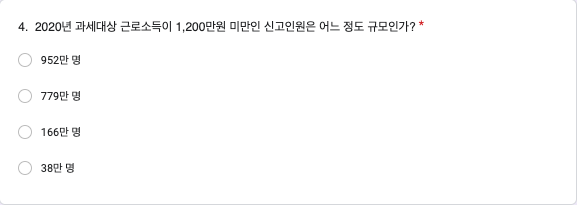
\includegraphics[width=0.75\linewidth]{./pics/Quiz230315_Q4}

\subsection{과세대상 근로소득 1,200만 원(집계표)}\label{uxacfcuxc138uxb300uxc0c1-uxadfcuxb85cuxc18cuxb4dd-1200uxb9cc-uxc6d0uxc9d1uxacc4uxd45c}

\begin{longtable}[]{@{}
  >{\raggedright\arraybackslash}p{(\columnwidth - 10\tabcolsep) * \real{0.1667}}
  >{\centering\arraybackslash}p{(\columnwidth - 10\tabcolsep) * \real{0.1528}}
  >{\centering\arraybackslash}p{(\columnwidth - 10\tabcolsep) * \real{0.1528}}
  >{\centering\arraybackslash}p{(\columnwidth - 10\tabcolsep) * \real{0.1528}}
  >{\centering\arraybackslash}p{(\columnwidth - 10\tabcolsep) * \real{0.1389}}
  >{\centering\arraybackslash}p{(\columnwidth - 10\tabcolsep) * \real{0.0833}}@{}}
\toprule\noalign{}
\begin{minipage}[b]{\linewidth}\raggedright
~
\end{minipage} & \begin{minipage}[b]{\linewidth}\centering
952만 명
\end{minipage} & \begin{minipage}[b]{\linewidth}\centering
779만 명
\end{minipage} & \begin{minipage}[b]{\linewidth}\centering
166만 명
\end{minipage} & \begin{minipage}[b]{\linewidth}\centering
38만 명
\end{minipage} & \begin{minipage}[b]{\linewidth}\centering
계
\end{minipage} \\
\midrule\noalign{}
\endhead
\bottomrule\noalign{}
\endlastfoot
\textbf{Red} & 158 & 71 & 39 & 9 & 277 \\
\textbf{Black} & 150 & 74 & 47 & 5 & 276 \\
\textbf{계} & 308 & 145 & 86 & 14 & 553 \\
\end{longtable}

\begin{longtable}[]{@{}
  >{\raggedleft\arraybackslash}p{(\columnwidth - 4\tabcolsep) * \real{0.2361}}
  >{\raggedleft\arraybackslash}p{(\columnwidth - 4\tabcolsep) * \real{0.0694}}
  >{\raggedleft\arraybackslash}p{(\columnwidth - 4\tabcolsep) * \real{0.1389}}@{}}
\caption{Pearson's Chi-squared test: \texttt{.}}\tabularnewline
\toprule\noalign{}
\begin{minipage}[b]{\linewidth}\raggedleft
Test statistic
\end{minipage} & \begin{minipage}[b]{\linewidth}\raggedleft
df
\end{minipage} & \begin{minipage}[b]{\linewidth}\raggedleft
P value
\end{minipage} \\
\midrule\noalign{}
\endfirsthead
\toprule\noalign{}
\begin{minipage}[b]{\linewidth}\raggedleft
Test statistic
\end{minipage} & \begin{minipage}[b]{\linewidth}\raggedleft
df
\end{minipage} & \begin{minipage}[b]{\linewidth}\raggedleft
P value
\end{minipage} \\
\midrule\noalign{}
\endhead
\bottomrule\noalign{}
\endlastfoot
2.155 & 3 & 0.5408 \\
\end{longtable}

Q4의 집계 결과가 Red, Black 간에 통계적으로 유의한 차이가 있는지 알아보기 위하여 카이제곱 테스트를 수행하였습니다.

그 결과 카이제곱 통계량은 2.155, 자유도는 3, p-value 는 0.5408이므로 Red, Black 간에 통계적으로 유의한 차이를 보이지 않습니다.

실제로 닮은 게 느껴집니까?

\subsection{과세대상 근로소득 1,200만 원(\%)}\label{uxacfcuxc138uxb300uxc0c1-uxadfcuxb85cuxc18cuxb4dd-1200uxb9cc-uxc6d0}

\begin{longtable}[]{@{}
  >{\centering\arraybackslash}p{(\columnwidth - 8\tabcolsep) * \real{0.1528}}
  >{\centering\arraybackslash}p{(\columnwidth - 8\tabcolsep) * \real{0.1528}}
  >{\centering\arraybackslash}p{(\columnwidth - 8\tabcolsep) * \real{0.1528}}
  >{\centering\arraybackslash}p{(\columnwidth - 8\tabcolsep) * \real{0.1389}}
  >{\centering\arraybackslash}p{(\columnwidth - 8\tabcolsep) * \real{0.1389}}@{}}
\toprule\noalign{}
\begin{minipage}[b]{\linewidth}\centering
952만 명
\end{minipage} & \begin{minipage}[b]{\linewidth}\centering
779만 명
\end{minipage} & \begin{minipage}[b]{\linewidth}\centering
166만 명
\end{minipage} & \begin{minipage}[b]{\linewidth}\centering
38만 명
\end{minipage} & \begin{minipage}[b]{\linewidth}\centering
계
\end{minipage} \\
\midrule\noalign{}
\endhead
\bottomrule\noalign{}
\endlastfoot
55.7 & 26.2 & 15.6 & 2.5 & 100.0 \\
\end{longtable}

정답률은 Red, Black 을 합하여 계산하는데, 55.7(\%) 입니다.

\section{Q5. 소득세 실효세율}\label{q5.-uxc18cuxb4dduxc138-uxc2e4uxd6a8uxc138uxc728}


\includegraphics[width=0.75\linewidth]{./pics/Quiz230315_Q5}

\subsection{소득세 실효세율(집계표)}\label{uxc18cuxb4dduxc138-uxc2e4uxd6a8uxc138uxc728uxc9d1uxacc4uxd45c}

\begin{longtable}[]{@{}
  >{\raggedright\arraybackslash}p{(\columnwidth - 10\tabcolsep) * \real{0.1667}}
  >{\raggedleft\arraybackslash}p{(\columnwidth - 10\tabcolsep) * \real{0.0972}}
  >{\raggedleft\arraybackslash}p{(\columnwidth - 10\tabcolsep) * \real{0.1111}}
  >{\raggedleft\arraybackslash}p{(\columnwidth - 10\tabcolsep) * \real{0.1111}}
  >{\raggedleft\arraybackslash}p{(\columnwidth - 10\tabcolsep) * \real{0.0972}}
  >{\centering\arraybackslash}p{(\columnwidth - 10\tabcolsep) * \real{0.0972}}@{}}
\toprule\noalign{}
\begin{minipage}[b]{\linewidth}\raggedright
~
\end{minipage} & \begin{minipage}[b]{\linewidth}\raggedleft
0.2\%
\end{minipage} & \begin{minipage}[b]{\linewidth}\raggedleft
15.1\%
\end{minipage} & \begin{minipage}[b]{\linewidth}\raggedleft
37.4\%
\end{minipage} & \begin{minipage}[b]{\linewidth}\raggedleft
5.9\%
\end{minipage} & \begin{minipage}[b]{\linewidth}\centering
계
\end{minipage} \\
\midrule\noalign{}
\endhead
\bottomrule\noalign{}
\endlastfoot
\textbf{Red} & 2 & 58 & 19 & 198 & 277 \\
\textbf{Black} & 8 & 48 & 16 & 204 & 276 \\
\textbf{계} & 10 & 106 & 35 & 402 & 553 \\
\end{longtable}

\begin{longtable}[]{@{}
  >{\raggedleft\arraybackslash}p{(\columnwidth - 4\tabcolsep) * \real{0.2361}}
  >{\raggedleft\arraybackslash}p{(\columnwidth - 4\tabcolsep) * \real{0.0694}}
  >{\raggedleft\arraybackslash}p{(\columnwidth - 4\tabcolsep) * \real{0.1389}}@{}}
\caption{Pearson's Chi-squared test: \texttt{.}}\tabularnewline
\toprule\noalign{}
\begin{minipage}[b]{\linewidth}\raggedleft
Test statistic
\end{minipage} & \begin{minipage}[b]{\linewidth}\raggedleft
df
\end{minipage} & \begin{minipage}[b]{\linewidth}\raggedleft
P value
\end{minipage} \\
\midrule\noalign{}
\endfirsthead
\toprule\noalign{}
\begin{minipage}[b]{\linewidth}\raggedleft
Test statistic
\end{minipage} & \begin{minipage}[b]{\linewidth}\raggedleft
df
\end{minipage} & \begin{minipage}[b]{\linewidth}\raggedleft
P value
\end{minipage} \\
\midrule\noalign{}
\endhead
\bottomrule\noalign{}
\endlastfoot
4.888 & 3 & 0.1802 \\
\end{longtable}

Q5의 집계 결과가 Red, Black 간에 통계적으로 유의한 차이가 있는지 알아보기 위하여 카이제곱 테스트를 수행하였습니다.

그 결과 카이제곱 통계량은 4.888, 자유도는 3, p-value 는 0.1802이므로 Red, Black 간에 통계적으로 유의한 차이를 보이지 않습니다.

실제로 닮은 게 느껴집니까?

\subsection{소득세 실효세율(\%)}\label{uxc18cuxb4dduxc138-uxc2e4uxd6a8uxc138uxc728}

\begin{longtable}[]{@{}
  >{\raggedleft\arraybackslash}p{(\columnwidth - 8\tabcolsep) * \real{0.0972}}
  >{\raggedleft\arraybackslash}p{(\columnwidth - 8\tabcolsep) * \real{0.1111}}
  >{\raggedleft\arraybackslash}p{(\columnwidth - 8\tabcolsep) * \real{0.1111}}
  >{\raggedleft\arraybackslash}p{(\columnwidth - 8\tabcolsep) * \real{0.0972}}
  >{\centering\arraybackslash}p{(\columnwidth - 8\tabcolsep) * \real{0.1111}}@{}}
\toprule\noalign{}
\begin{minipage}[b]{\linewidth}\raggedleft
0.2\%
\end{minipage} & \begin{minipage}[b]{\linewidth}\raggedleft
15.1\%
\end{minipage} & \begin{minipage}[b]{\linewidth}\raggedleft
37.4\%
\end{minipage} & \begin{minipage}[b]{\linewidth}\raggedleft
5.9\%
\end{minipage} & \begin{minipage}[b]{\linewidth}\centering
계
\end{minipage} \\
\midrule\noalign{}
\endhead
\bottomrule\noalign{}
\endlastfoot
1.8 & 19.2 & 6.3 & 72.7 & 100.0 \\
\end{longtable}

정답률은 Red, Black 을 합하여 계산하는데, 72.7(\%) 입니다.

\section{Q6. 기업규모별 과세 현황}\label{q6.-uxae30uxc5c5uxaddcuxbaa8uxbcc4-uxacfcuxc138-uxd604uxd669}

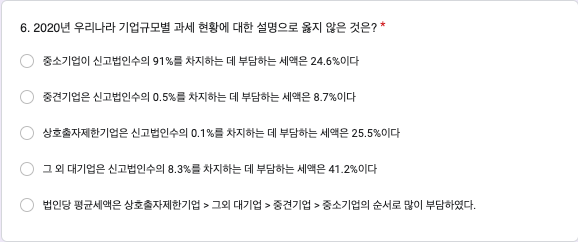
\includegraphics[width=0.75\linewidth]{./pics/Quiz230315_Q6}

\subsection{기업규모별 과세 현황(집계표)}\label{uxae30uxc5c5uxaddcuxbaa8uxbcc4-uxacfcuxc138-uxd604uxd669uxc9d1uxacc4uxd45c}

\begin{longtable}[]{@{}
  >{\raggedright\arraybackslash}p{(\columnwidth - 12\tabcolsep) * \real{0.0678}}
  >{\centering\arraybackslash}p{(\columnwidth - 12\tabcolsep) * \real{0.1808}}
  >{\centering\arraybackslash}p{(\columnwidth - 12\tabcolsep) * \real{0.1864}}
  >{\centering\arraybackslash}p{(\columnwidth - 12\tabcolsep) * \real{0.1751}}
  >{\centering\arraybackslash}p{(\columnwidth - 12\tabcolsep) * \real{0.1695}}
  >{\centering\arraybackslash}p{(\columnwidth - 12\tabcolsep) * \real{0.1864}}
  >{\centering\arraybackslash}p{(\columnwidth - 12\tabcolsep) * \real{0.0339}}@{}}
\toprule\noalign{}
\begin{minipage}[b]{\linewidth}\raggedright
~
\end{minipage} & \begin{minipage}[b]{\linewidth}\centering
중소기업이 신고법인수의 91\%를
차지하는 데 부담하는 세액은
24.6\%이다
\end{minipage} & \begin{minipage}[b]{\linewidth}\centering
중견기업은 신고법인수의 0.5\%를
차지하는 데 부담하는 세액은
8.7\%이다
\end{minipage} & \begin{minipage}[b]{\linewidth}\centering
상호출자제한기업은
신고법인수의 0.1\%를 차지하는
데 부담하는 세액은 25.5\%이다
\end{minipage} & \begin{minipage}[b]{\linewidth}\centering
그 외 대기업은 신고법인수의
8.3\%를 차지하는 데 부담하는
세액은 41.2\%이다
\end{minipage} & \begin{minipage}[b]{\linewidth}\centering
법인당 평균세액은
상호출자제한기업 \textgreater{} 그외 대기업
\textgreater{} 중견기업 \textgreater{} 중소기업의 순서로
많이 부담하였다.
\end{minipage} & \begin{minipage}[b]{\linewidth}\centering
계
\end{minipage} \\
\midrule\noalign{}
\endhead
\bottomrule\noalign{}
\endlastfoot
\textbf{Red} & 14 & 37 & 38 & 50 & 138 & 277 \\
\textbf{Black} & 18 & 33 & 21 & 61 & 143 & 276 \\
\textbf{계} & 32 & 70 & 59 & 111 & 281 & 553 \\
\end{longtable}

\begin{longtable}[]{@{}
  >{\raggedleft\arraybackslash}p{(\columnwidth - 4\tabcolsep) * \real{0.2361}}
  >{\raggedleft\arraybackslash}p{(\columnwidth - 4\tabcolsep) * \real{0.0694}}
  >{\raggedleft\arraybackslash}p{(\columnwidth - 4\tabcolsep) * \real{0.1389}}@{}}
\caption{Pearson's Chi-squared test: \texttt{.}}\tabularnewline
\toprule\noalign{}
\begin{minipage}[b]{\linewidth}\raggedleft
Test statistic
\end{minipage} & \begin{minipage}[b]{\linewidth}\raggedleft
df
\end{minipage} & \begin{minipage}[b]{\linewidth}\raggedleft
P value
\end{minipage} \\
\midrule\noalign{}
\endfirsthead
\toprule\noalign{}
\begin{minipage}[b]{\linewidth}\raggedleft
Test statistic
\end{minipage} & \begin{minipage}[b]{\linewidth}\raggedleft
df
\end{minipage} & \begin{minipage}[b]{\linewidth}\raggedleft
P value
\end{minipage} \\
\midrule\noalign{}
\endhead
\bottomrule\noalign{}
\endlastfoot
6.804 & 4 & 0.1466 \\
\end{longtable}

Q6의 집계 결과가 Red, Black 간에 통계적으로 유의한 차이가 있는지 알아보기 위하여 카이제곱 테스트를 수행하였습니다.

그 결과 카이제곱 통계량은 6.804, 자유도는 4, p-value 는 0.1466이므로 Red, Black 간에 통계적으로 유의한 차이를 보이지 않습니다.

실제로 닮은 게 느껴집니까?

\subsection{기업규모별 과세 현황(\%)}\label{uxae30uxc5c5uxaddcuxbaa8uxbcc4-uxacfcuxc138-uxd604uxd669}

\begin{longtable}[]{@{}
  >{\centering\arraybackslash}p{(\columnwidth - 10\tabcolsep) * \real{0.1916}}
  >{\centering\arraybackslash}p{(\columnwidth - 10\tabcolsep) * \real{0.1976}}
  >{\centering\arraybackslash}p{(\columnwidth - 10\tabcolsep) * \real{0.1856}}
  >{\centering\arraybackslash}p{(\columnwidth - 10\tabcolsep) * \real{0.1796}}
  >{\centering\arraybackslash}p{(\columnwidth - 10\tabcolsep) * \real{0.1976}}
  >{\centering\arraybackslash}p{(\columnwidth - 10\tabcolsep) * \real{0.0479}}@{}}
\toprule\noalign{}
\begin{minipage}[b]{\linewidth}\centering
중소기업이 신고법인수의 91\%를
차지하는 데 부담하는 세액은
24.6\%이다
\end{minipage} & \begin{minipage}[b]{\linewidth}\centering
중견기업은 신고법인수의 0.5\%를
차지하는 데 부담하는 세액은
8.7\%이다
\end{minipage} & \begin{minipage}[b]{\linewidth}\centering
상호출자제한기업은
신고법인수의 0.1\%를 차지하는
데 부담하는 세액은 25.5\%이다
\end{minipage} & \begin{minipage}[b]{\linewidth}\centering
그 외 대기업은 신고법인수의
8.3\%를 차지하는 데 부담하는
세액은 41.2\%이다
\end{minipage} & \begin{minipage}[b]{\linewidth}\centering
법인당 평균세액은
상호출자제한기업 \textgreater{} 그외 대기업
\textgreater{} 중견기업 \textgreater{} 중소기업의 순서로
많이 부담하였다.
\end{minipage} & \begin{minipage}[b]{\linewidth}\centering
계
\end{minipage} \\
\midrule\noalign{}
\endhead
\bottomrule\noalign{}
\endlastfoot
5.8 & 12.7 & 10.7 & 20.1 & 50.8 & 100.0 \\
\end{longtable}

정답률은 Red, Black 을 합하여 계산하는데, 50.8(\%) 입니다.

\section{Q7. 국민부담률 적정 수준 : 아일랜드와 OECD 평균}\label{q7.-uxad6duxbbfcuxbd80uxb2f4uxb960-uxc801uxc815-uxc218uxc900-uxc544uxc77cuxb79cuxb4dcuxc640-oecd-uxd3c9uxade0}

질문 내용에 의도하는 바를 담으면 어떨까요?

OECD 국가 중 국민부담률이 매우 낮은 편인 아일랜드의 사례를 들어서 감세정책이 가져온 긍정적인 효과에 대해서 설명하고 우리나라의 바람직한 조정 방향은 무엇이냐고 묻는 것을 Red, 감세 정책이 가져온 부정적인 효과에 대해서 설명하고 우리나라의 바람직한 조정 방향은 무엇이냐고 묻는 것을 Black 에 배치했을 때, 설명이 응답에 영향을 미치지 않으면 Red 와 Black에 차이가 없어야 할텐데 집계결과는 어떻게 나오고 있나요?

분명히 영향을 미치고 있는 것으로 보입니다.

통계적으로 매우 유의한 차이가 관찰되고 있습니다.

감세정책의 효과가 긍정적이라고 설명한 Red 에서는 낮춰야 한다는 응답이, 감세정책의 효과가 부정적이라고 설명한 Black 에서는 높여야 한다는 응답이 높게 나온 것을 볼 수 있고, 따라서 p-value 가 엄청나게 작은 값을 보여주고 있습니다.

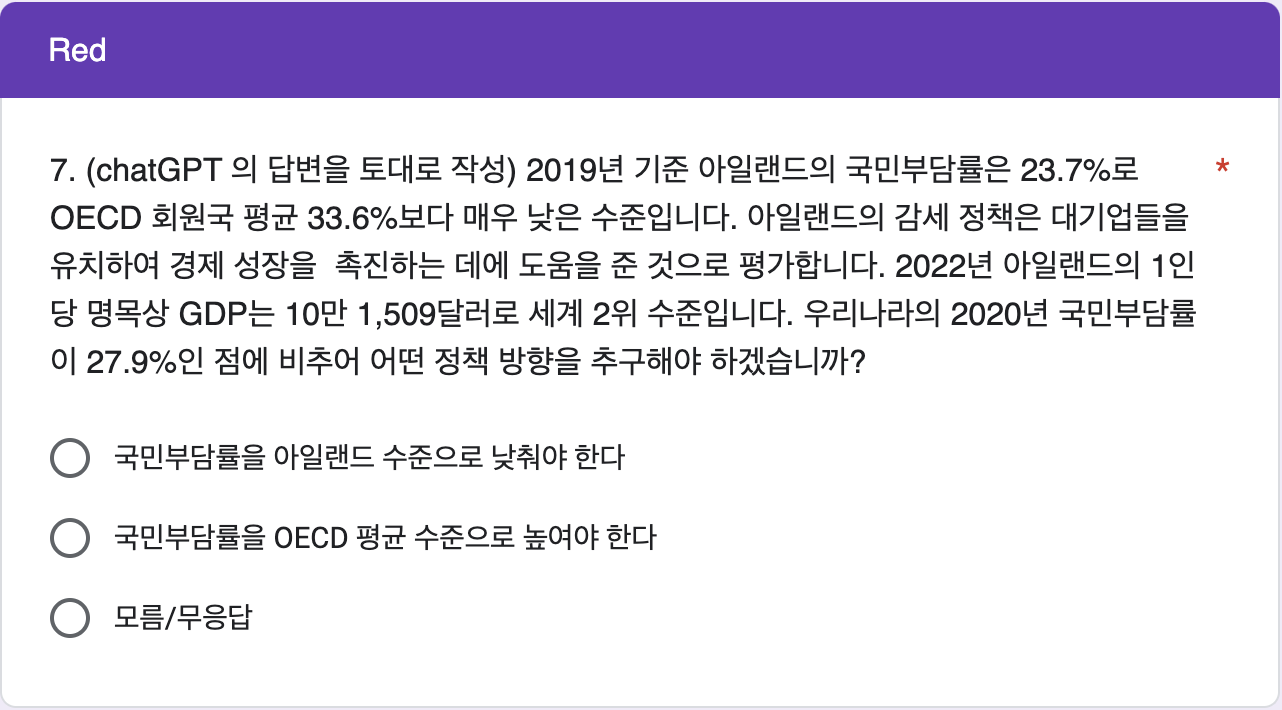
\includegraphics[width=0.67\linewidth]{./pics/Quiz240315_Q7_Red}

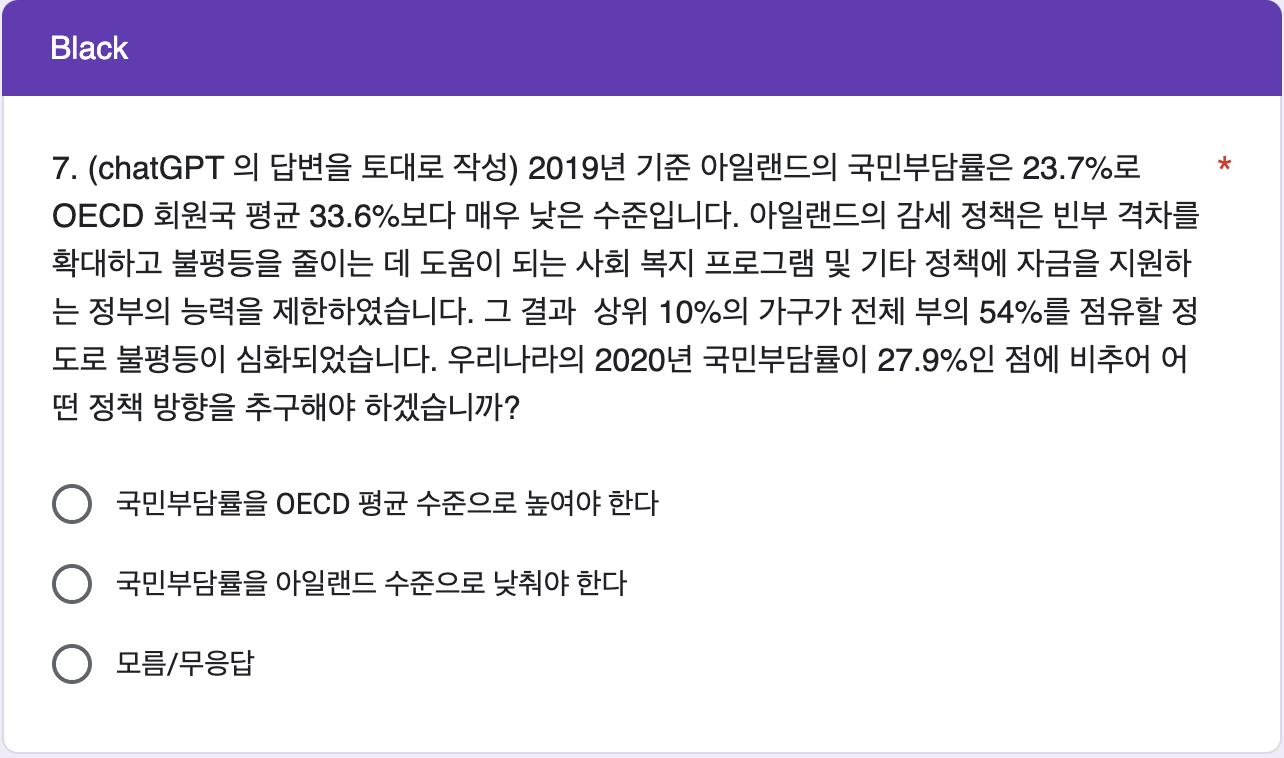
\includegraphics[width=0.67\linewidth]{./pics/Quiz240315_Q7_Black}

\subsection{집계표}\label{uxc9d1uxacc4uxd45c-1}

\begin{longtable}[]{@{}
  >{\raggedright\arraybackslash}p{(\columnwidth - 8\tabcolsep) * \real{0.3766}}
  >{\centering\arraybackslash}p{(\columnwidth - 8\tabcolsep) * \real{0.1818}}
  >{\centering\arraybackslash}p{(\columnwidth - 8\tabcolsep) * \real{0.1818}}
  >{\centering\arraybackslash}p{(\columnwidth - 8\tabcolsep) * \real{0.1818}}
  >{\centering\arraybackslash}p{(\columnwidth - 8\tabcolsep) * \real{0.0779}}@{}}
\toprule\noalign{}
\begin{minipage}[b]{\linewidth}\raggedright
~
\end{minipage} & \begin{minipage}[b]{\linewidth}\centering
낮춰야 한다
\end{minipage} & \begin{minipage}[b]{\linewidth}\centering
높여야 한다
\end{minipage} & \begin{minipage}[b]{\linewidth}\centering
모름/무응답
\end{minipage} & \begin{minipage}[b]{\linewidth}\centering
계
\end{minipage} \\
\midrule\noalign{}
\endhead
\bottomrule\noalign{}
\endlastfoot
\textbf{Red(감세의 긍정적효과
설명)} & 90 & 120 & 67 & 277 \\
\textbf{Black(감세의 부정적 효과
설명)} & 46 & 168 & 62 & 276 \\
\textbf{계} & 136 & 288 & 129 & 553 \\
\end{longtable}

\begin{longtable}[]{@{}
  >{\raggedleft\arraybackslash}p{(\columnwidth - 4\tabcolsep) * \real{0.2361}}
  >{\raggedleft\arraybackslash}p{(\columnwidth - 4\tabcolsep) * \real{0.0694}}
  >{\raggedleft\arraybackslash}p{(\columnwidth - 4\tabcolsep) * \real{0.2500}}@{}}
\caption{Pearson's Chi-squared test: \texttt{.}}\tabularnewline
\toprule\noalign{}
\begin{minipage}[b]{\linewidth}\raggedleft
Test statistic
\end{minipage} & \begin{minipage}[b]{\linewidth}\raggedleft
df
\end{minipage} & \begin{minipage}[b]{\linewidth}\raggedleft
P value
\end{minipage} \\
\midrule\noalign{}
\endfirsthead
\toprule\noalign{}
\begin{minipage}[b]{\linewidth}\raggedleft
Test statistic
\end{minipage} & \begin{minipage}[b]{\linewidth}\raggedleft
df
\end{minipage} & \begin{minipage}[b]{\linewidth}\raggedleft
P value
\end{minipage} \\
\midrule\noalign{}
\endhead
\bottomrule\noalign{}
\endlastfoot
22.43 & 2 & 1.349e-05 * * * \\
\end{longtable}

Q7의 Red에는 아일랜드의 사례에서 감세 정책의 긍정적 측면을 설명한 후 우리나라 조세 정책의 방향에 대하여 물었을 때, 277명이 응답한 가운데 90명이 우리나라의 국민부담률을 아일랜드 수준으로 ``낮춰야 한다''는 반응을 보이고, 120명이 OECD평균 수준으로 ``높여야 한다''는 반응을 보입니다.

Black은 같은 아일랜드의 사례에서 감세 정책의 부정적 측면을 설명한 후 우리나라 조세 정책의 방향에 대하여 물었을 떄, 276명이 응답한 가운데 46명이 우리나라의 국민부담률을 아일랜드 수준으로 ``낮춰야 한다''는 반응을 보이고, 168명이 OECD 평균 수준으로 ``높여야 한다''는 반응을 보입니다.

그리고 ``모름/무응답''에 답한 인원은 Red에 67명, Black 에 62명이 응답하였습니다.

우연일까요?

모름/무응답에 있어서는 Red, Black이 몹시 닮았습니다.

카이제곱 테스트는 이와 같은 상황에서 감세정책의 긍정적 측면을 부각시킨 경우와 부정적 측면을 부각시킨 경우에 그 차이가 통계적으로 매우, 매우, \ldots{} 유의하다는 것을 보여 줍니다.

카이제곱 통계량은 22.427, 자유도는 2, p-value 는 1.3e-05으로
감세정책의 어떤 측면을 설명하느냐에 따라 반응이 다르게 나온다는 것을 보여줍니다.

여기서 질문 내용에 의도하는 바를 담더라도 응답에 영향을 끼치지 않는다고 가정합니다.

랜덤화의 효과로 Red, Black 의 응답은 닮게 마련입니다.

즉, 통계적으로 유의한 차이를 보이지 않게 됩니다.

그러나 실제로 관찰된 카이제곱 통계값의 P-value 는 0.05보다 매우 작은 값입니다.

따라서, 질문 내용에 의도하는 바를 담더라도 영향을 끼치지 않는다는 가정은 잘못된 것이죠.

이러한 논증 방식을 귀류법이라고 합니다.

\subsection{\% 비교}\label{uxbe44uxad50-1}

\begin{longtable}[]{@{}
  >{\raggedright\arraybackslash}p{(\columnwidth - 8\tabcolsep) * \real{0.3671}}
  >{\centering\arraybackslash}p{(\columnwidth - 8\tabcolsep) * \real{0.1772}}
  >{\centering\arraybackslash}p{(\columnwidth - 8\tabcolsep) * \real{0.1772}}
  >{\centering\arraybackslash}p{(\columnwidth - 8\tabcolsep) * \real{0.1772}}
  >{\centering\arraybackslash}p{(\columnwidth - 8\tabcolsep) * \real{0.1013}}@{}}
\toprule\noalign{}
\begin{minipage}[b]{\linewidth}\raggedright
~
\end{minipage} & \begin{minipage}[b]{\linewidth}\centering
낮춰야 한다
\end{minipage} & \begin{minipage}[b]{\linewidth}\centering
높여야 한다
\end{minipage} & \begin{minipage}[b]{\linewidth}\centering
모름/무응답
\end{minipage} & \begin{minipage}[b]{\linewidth}\centering
계
\end{minipage} \\
\midrule\noalign{}
\endhead
\bottomrule\noalign{}
\endlastfoot
\textbf{Red(감세의 긍정적효과
설명)} & 32.5 & 43.3 & 24.2 & 100.0 \\
\textbf{Black(감세의 부정적 효과
설명)} & 16.7 & 60.9 & 22.5 & 100.0 \\
\end{longtable}

감세정책의 긍정적 측면을 설명한 Red에서 우리나라의 국민부담률을 ``낮춰야 한다''고 응답하는사람들의 백분율, 32.5(\%)은 ``높여야 한다''고 응답하는 사람들의 백분율, 43.3(\%) 보다 높습니다.

반면 감세정책의 부정적 측면을 설명한 Black에서 우리나라의 국민 부담률을 ``낮춰야 한다''고 응답하는 사람들의 백분율, 16.7(\%)은 ``높여야 한다''고 응답하는 사람들의 백분율, 60.9(\%) 보다 훨씬 적습니다.

어느 정책의 긍정적 측면을 설명하느냐, 부정적 측면을 설명하느냐에 따라 반응이 달라진다는 것을 잘 알 수 있습니다.

Red 와 Black 이 워낙 차이가 나지만 전체적으로 어느 정도가 우리나라의 국민부담률을 ``낮춰야 한다''하고 어느 정도가 ``높여야 한다''고 응답하였는지 합쳐 보겠습니다.

\subsection{\% 합계}\label{uxd569uxacc4}

\begin{longtable}[]{@{}
  >{\centering\arraybackslash}p{(\columnwidth - 6\tabcolsep) * \real{0.1944}}
  >{\centering\arraybackslash}p{(\columnwidth - 6\tabcolsep) * \real{0.1944}}
  >{\centering\arraybackslash}p{(\columnwidth - 6\tabcolsep) * \real{0.1944}}
  >{\centering\arraybackslash}p{(\columnwidth - 6\tabcolsep) * \real{0.1111}}@{}}
\toprule\noalign{}
\begin{minipage}[b]{\linewidth}\centering
낮춰야 한다
\end{minipage} & \begin{minipage}[b]{\linewidth}\centering
높여야 한다
\end{minipage} & \begin{minipage}[b]{\linewidth}\centering
모름/무응답
\end{minipage} & \begin{minipage}[b]{\linewidth}\centering
계
\end{minipage} \\
\midrule\noalign{}
\endhead
\bottomrule\noalign{}
\endlastfoot
24.6 & 52.1 & 23.3 & 100.0 \\
\end{longtable}

우리나라의 국민부담률을 ``낮춰야 한다''고 응답한 백분율은 Red, Black 합쳐서 24.6(\%)(으)로 우리나라의 국민부담률을 '높여야한다''고 응답한 백분율, 52.1(\%) 보다 상당히 적습니다.

다만, 모름/무응답이 23.3(\%)로 적지 않습니다.

\subsection{Mosaic Plot}\label{mosaic-plot-4}

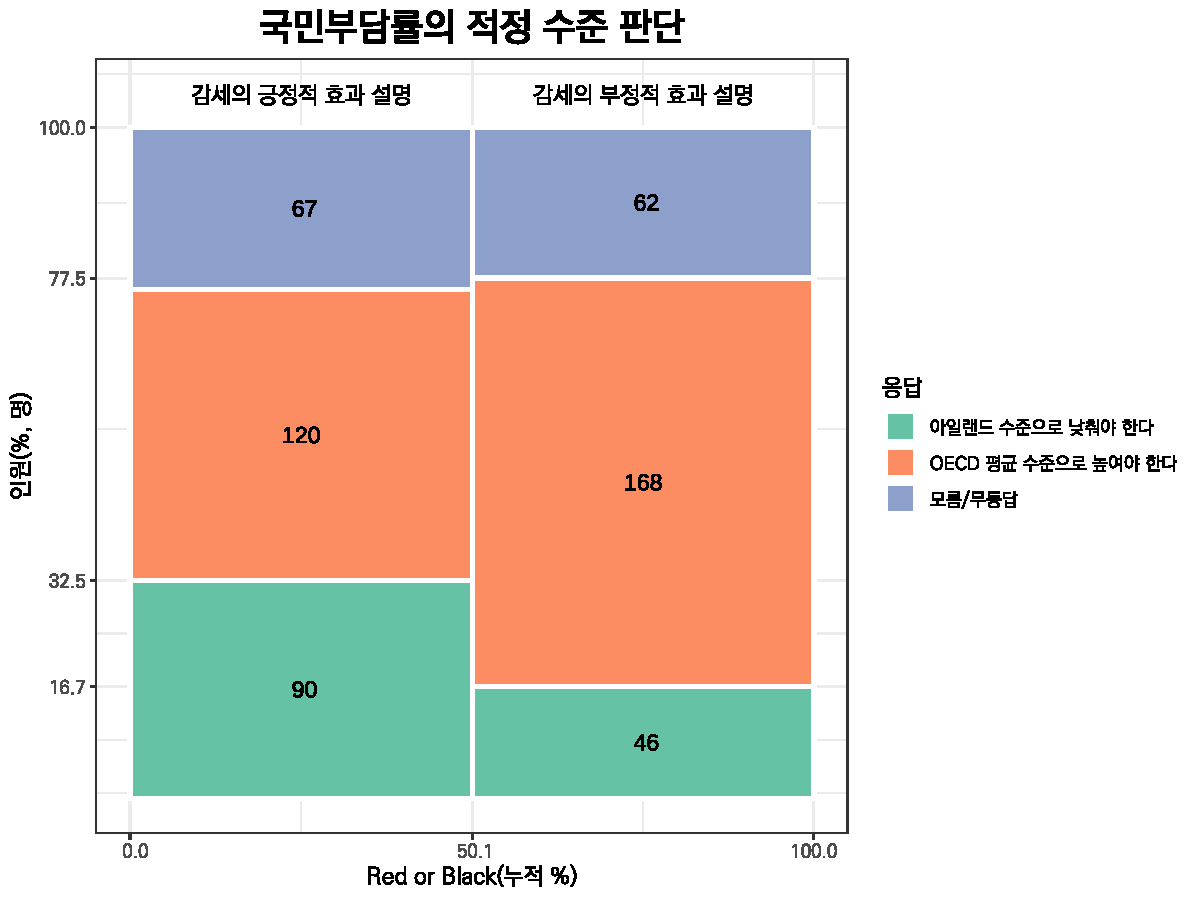
\includegraphics{_main_files/figure-latex/unnamed-chunk-72-1.pdf}

Mosaic Plot 은 이 집계결과를 시각적으로 잘 보여줍니다.

감세정책의 긍정적 측면을 설명한 Red 에서 우리나라의 국민부담률을 ``낮춰야 한다''고 응답한 백분율이 높고, 감세정책의 부정적 측면을 설명한 Black 에서 우리나라의 국민부담률을 ``높여야 한다''고 응답한 백분율이 월등히 높은 것을 시각적으로 알 수 있습니다.

\section{마감 시간으로부터 제출 시간의 분포}\label{uxb9c8uxac10-uxc2dcuxac04uxc73cuxb85cuxbd80uxd130-uxc81cuxcd9c-uxc2dcuxac04uxc758-uxbd84uxd3ec-2}

\subsection{분포표}\label{uxbd84uxd3ecuxd45c-3}

\begin{longtable}[]{@{}
  >{\raggedright\arraybackslash}p{(\columnwidth - 30\tabcolsep) * \real{0.0863}}
  >{\raggedleft\arraybackslash}p{(\columnwidth - 30\tabcolsep) * \real{0.0576}}
  >{\raggedleft\arraybackslash}p{(\columnwidth - 30\tabcolsep) * \real{0.0576}}
  >{\raggedleft\arraybackslash}p{(\columnwidth - 30\tabcolsep) * \real{0.0576}}
  >{\raggedleft\arraybackslash}p{(\columnwidth - 30\tabcolsep) * \real{0.0576}}
  >{\raggedleft\arraybackslash}p{(\columnwidth - 30\tabcolsep) * \real{0.0576}}
  >{\raggedleft\arraybackslash}p{(\columnwidth - 30\tabcolsep) * \real{0.0576}}
  >{\raggedleft\arraybackslash}p{(\columnwidth - 30\tabcolsep) * \real{0.0576}}
  >{\raggedleft\arraybackslash}p{(\columnwidth - 30\tabcolsep) * \real{0.0576}}
  >{\raggedleft\arraybackslash}p{(\columnwidth - 30\tabcolsep) * \real{0.0576}}
  >{\raggedleft\arraybackslash}p{(\columnwidth - 30\tabcolsep) * \real{0.0647}}
  >{\raggedleft\arraybackslash}p{(\columnwidth - 30\tabcolsep) * \real{0.0719}}
  >{\raggedleft\arraybackslash}p{(\columnwidth - 30\tabcolsep) * \real{0.0719}}
  >{\raggedleft\arraybackslash}p{(\columnwidth - 30\tabcolsep) * \real{0.0719}}
  >{\raggedleft\arraybackslash}p{(\columnwidth - 30\tabcolsep) * \real{0.0719}}
  >{\centering\arraybackslash}p{(\columnwidth - 30\tabcolsep) * \real{0.0432}}@{}}
\caption{일 단위}\tabularnewline
\toprule\noalign{}
\begin{minipage}[b]{\linewidth}\raggedright
~
\end{minipage} & \begin{minipage}[b]{\linewidth}\raggedleft
{[}0,1{]}
\end{minipage} & \begin{minipage}[b]{\linewidth}\raggedleft
(1,2{]}
\end{minipage} & \begin{minipage}[b]{\linewidth}\raggedleft
(2,3{]}
\end{minipage} & \begin{minipage}[b]{\linewidth}\raggedleft
(3,4{]}
\end{minipage} & \begin{minipage}[b]{\linewidth}\raggedleft
(4,5{]}
\end{minipage} & \begin{minipage}[b]{\linewidth}\raggedleft
(5,6{]}
\end{minipage} & \begin{minipage}[b]{\linewidth}\raggedleft
(6,7{]}
\end{minipage} & \begin{minipage}[b]{\linewidth}\raggedleft
(7,8{]}
\end{minipage} & \begin{minipage}[b]{\linewidth}\raggedleft
(8,9{]}
\end{minipage} & \begin{minipage}[b]{\linewidth}\raggedleft
(9,10{]}
\end{minipage} & \begin{minipage}[b]{\linewidth}\raggedleft
(10,11{]}
\end{minipage} & \begin{minipage}[b]{\linewidth}\raggedleft
(11,12{]}
\end{minipage} & \begin{minipage}[b]{\linewidth}\raggedleft
(12,13{]}
\end{minipage} & \begin{minipage}[b]{\linewidth}\raggedleft
(13,14{]}
\end{minipage} & \begin{minipage}[b]{\linewidth}\centering
계
\end{minipage} \\
\midrule\noalign{}
\endfirsthead
\toprule\noalign{}
\begin{minipage}[b]{\linewidth}\raggedright
~
\end{minipage} & \begin{minipage}[b]{\linewidth}\raggedleft
{[}0,1{]}
\end{minipage} & \begin{minipage}[b]{\linewidth}\raggedleft
(1,2{]}
\end{minipage} & \begin{minipage}[b]{\linewidth}\raggedleft
(2,3{]}
\end{minipage} & \begin{minipage}[b]{\linewidth}\raggedleft
(3,4{]}
\end{minipage} & \begin{minipage}[b]{\linewidth}\raggedleft
(4,5{]}
\end{minipage} & \begin{minipage}[b]{\linewidth}\raggedleft
(5,6{]}
\end{minipage} & \begin{minipage}[b]{\linewidth}\raggedleft
(6,7{]}
\end{minipage} & \begin{minipage}[b]{\linewidth}\raggedleft
(7,8{]}
\end{minipage} & \begin{minipage}[b]{\linewidth}\raggedleft
(8,9{]}
\end{minipage} & \begin{minipage}[b]{\linewidth}\raggedleft
(9,10{]}
\end{minipage} & \begin{minipage}[b]{\linewidth}\raggedleft
(10,11{]}
\end{minipage} & \begin{minipage}[b]{\linewidth}\raggedleft
(11,12{]}
\end{minipage} & \begin{minipage}[b]{\linewidth}\raggedleft
(12,13{]}
\end{minipage} & \begin{minipage}[b]{\linewidth}\raggedleft
(13,14{]}
\end{minipage} & \begin{minipage}[b]{\linewidth}\centering
계
\end{minipage} \\
\midrule\noalign{}
\endhead
\bottomrule\noalign{}
\endlastfoot
\textbf{Red} & 71 & 12 & 6 & 8 & 4 & 6 & 16 & 48 & 20 & 14 & 18 & 17 & 16 & 21 & 277 \\
\textbf{Black} & 64 & 14 & 3 & 6 & 10 & 4 & 4 & 47 & 30 & 18 & 12 & 17 & 22 & 25 & 276 \\
\textbf{계} & 135 & 26 & 9 & 14 & 14 & 10 & 20 & 95 & 50 & 32 & 30 & 34 & 38 & 46 & 553 \\
\end{longtable}

분포표로부터 두 가지 문제를 살펴보겠습니다.

첫째, 날마다 고르게 제출하는가?

둘째, Red, Black 간에 통계적으로 유의한 차이가 있는가?

각 문제를 살펴보기 위해서는 분포표의 일부분을 대상으로 카이제곱 테스트를 수행합니다.

\subsection{날마다 고르게 제출하는가?}\label{uxb0a0uxb9c8uxb2e4-uxace0uxb974uxac8c-uxc81cuxcd9cuxd558uxb294uxac00-2}

\begin{longtable}[]{@{}
  >{\raggedleft\arraybackslash}p{(\columnwidth - 26\tabcolsep) * \real{0.0661}}
  >{\raggedleft\arraybackslash}p{(\columnwidth - 26\tabcolsep) * \real{0.0661}}
  >{\raggedleft\arraybackslash}p{(\columnwidth - 26\tabcolsep) * \real{0.0661}}
  >{\raggedleft\arraybackslash}p{(\columnwidth - 26\tabcolsep) * \real{0.0661}}
  >{\raggedleft\arraybackslash}p{(\columnwidth - 26\tabcolsep) * \real{0.0661}}
  >{\raggedleft\arraybackslash}p{(\columnwidth - 26\tabcolsep) * \real{0.0661}}
  >{\raggedleft\arraybackslash}p{(\columnwidth - 26\tabcolsep) * \real{0.0661}}
  >{\raggedleft\arraybackslash}p{(\columnwidth - 26\tabcolsep) * \real{0.0661}}
  >{\raggedleft\arraybackslash}p{(\columnwidth - 26\tabcolsep) * \real{0.0661}}
  >{\raggedleft\arraybackslash}p{(\columnwidth - 26\tabcolsep) * \real{0.0744}}
  >{\raggedleft\arraybackslash}p{(\columnwidth - 26\tabcolsep) * \real{0.0826}}
  >{\raggedleft\arraybackslash}p{(\columnwidth - 26\tabcolsep) * \real{0.0826}}
  >{\raggedleft\arraybackslash}p{(\columnwidth - 26\tabcolsep) * \real{0.0826}}
  >{\raggedleft\arraybackslash}p{(\columnwidth - 26\tabcolsep) * \real{0.0826}}@{}}
\toprule\noalign{}
\begin{minipage}[b]{\linewidth}\raggedleft
{[}0,1{]}
\end{minipage} & \begin{minipage}[b]{\linewidth}\raggedleft
(1,2{]}
\end{minipage} & \begin{minipage}[b]{\linewidth}\raggedleft
(2,3{]}
\end{minipage} & \begin{minipage}[b]{\linewidth}\raggedleft
(3,4{]}
\end{minipage} & \begin{minipage}[b]{\linewidth}\raggedleft
(4,5{]}
\end{minipage} & \begin{minipage}[b]{\linewidth}\raggedleft
(5,6{]}
\end{minipage} & \begin{minipage}[b]{\linewidth}\raggedleft
(6,7{]}
\end{minipage} & \begin{minipage}[b]{\linewidth}\raggedleft
(7,8{]}
\end{minipage} & \begin{minipage}[b]{\linewidth}\raggedleft
(8,9{]}
\end{minipage} & \begin{minipage}[b]{\linewidth}\raggedleft
(9,10{]}
\end{minipage} & \begin{minipage}[b]{\linewidth}\raggedleft
(10,11{]}
\end{minipage} & \begin{minipage}[b]{\linewidth}\raggedleft
(11,12{]}
\end{minipage} & \begin{minipage}[b]{\linewidth}\raggedleft
(12,13{]}
\end{minipage} & \begin{minipage}[b]{\linewidth}\raggedleft
(13,14{]}
\end{minipage} \\
\midrule\noalign{}
\endhead
\bottomrule\noalign{}
\endlastfoot
135 & 26 & 9 & 14 & 14 & 10 & 20 & 95 & 50 & 32 & 30 & 34 & 38 & 46 \\
\end{longtable}

\begin{longtable}[]{@{}
  >{\raggedleft\arraybackslash}p{(\columnwidth - 4\tabcolsep) * \real{0.2361}}
  >{\raggedleft\arraybackslash}p{(\columnwidth - 4\tabcolsep) * \real{0.0694}}
  >{\raggedleft\arraybackslash}p{(\columnwidth - 4\tabcolsep) * \real{0.2500}}@{}}
\caption{Chi-squared test for given probabilities: \texttt{.}}\tabularnewline
\toprule\noalign{}
\begin{minipage}[b]{\linewidth}\raggedleft
Test statistic
\end{minipage} & \begin{minipage}[b]{\linewidth}\raggedleft
df
\end{minipage} & \begin{minipage}[b]{\linewidth}\raggedleft
P value
\end{minipage} \\
\midrule\noalign{}
\endfirsthead
\toprule\noalign{}
\begin{minipage}[b]{\linewidth}\raggedleft
Test statistic
\end{minipage} & \begin{minipage}[b]{\linewidth}\raggedleft
df
\end{minipage} & \begin{minipage}[b]{\linewidth}\raggedleft
P value
\end{minipage} \\
\midrule\noalign{}
\endhead
\bottomrule\noalign{}
\endlastfoot
410 & 13 & 1.714e-79 * * * \\
\end{longtable}

날마다 고르게 제출하는지 알아 보았습니다.

분포표의 ``계''행에서 '계'열을 제외하고 카이제곱테스트를 수행합니다.

분포표 만으로도 쉽게 파악할 수 있지만 카이제곱테스트가 명확히 해 줍니다.

카이제곱 통계량은 410.01, 자유도는 13.00, p-value 는 1.7e-79 이므로 결코 고르게 제출한다고 말할 수 없겠습니다.

막대그래프로 살펴 보겠습니다.

\subsection{막대그래프}\label{uxb9c9uxb300uxadf8uxb798uxd504-3}

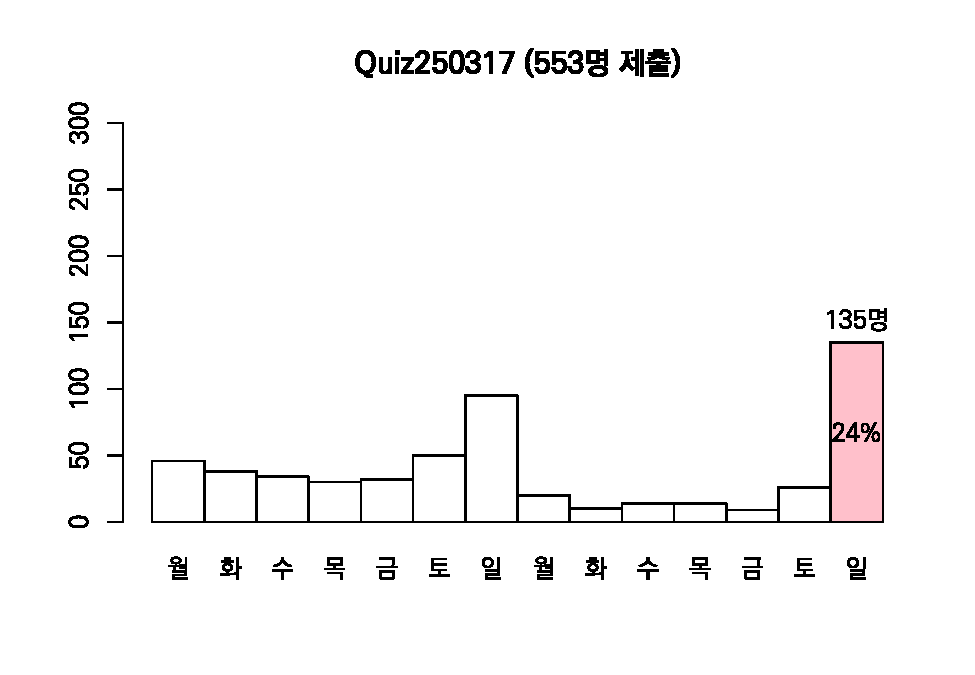
\includegraphics{_main_files/figure-latex/unnamed-chunk-75-1.pdf}

막대그래프는 총 제출인원 553(명) 중에 135(명), 24(\%)가 마감일에 몰리는 것을 명확히 보여주고 있습니다.

\subsection{Red, Black 간에 닮았는가?}\label{red-black-uxac04uxc5d0-uxb2eeuxc558uxb294uxac00-2}

\begin{longtable}[]{@{}
  >{\raggedright\arraybackslash}p{(\columnwidth - 28\tabcolsep) * \real{0.0902}}
  >{\raggedleft\arraybackslash}p{(\columnwidth - 28\tabcolsep) * \real{0.0602}}
  >{\raggedleft\arraybackslash}p{(\columnwidth - 28\tabcolsep) * \real{0.0602}}
  >{\raggedleft\arraybackslash}p{(\columnwidth - 28\tabcolsep) * \real{0.0602}}
  >{\raggedleft\arraybackslash}p{(\columnwidth - 28\tabcolsep) * \real{0.0602}}
  >{\raggedleft\arraybackslash}p{(\columnwidth - 28\tabcolsep) * \real{0.0602}}
  >{\raggedleft\arraybackslash}p{(\columnwidth - 28\tabcolsep) * \real{0.0602}}
  >{\raggedleft\arraybackslash}p{(\columnwidth - 28\tabcolsep) * \real{0.0602}}
  >{\raggedleft\arraybackslash}p{(\columnwidth - 28\tabcolsep) * \real{0.0602}}
  >{\raggedleft\arraybackslash}p{(\columnwidth - 28\tabcolsep) * \real{0.0602}}
  >{\raggedleft\arraybackslash}p{(\columnwidth - 28\tabcolsep) * \real{0.0677}}
  >{\raggedleft\arraybackslash}p{(\columnwidth - 28\tabcolsep) * \real{0.0752}}
  >{\raggedleft\arraybackslash}p{(\columnwidth - 28\tabcolsep) * \real{0.0752}}
  >{\raggedleft\arraybackslash}p{(\columnwidth - 28\tabcolsep) * \real{0.0752}}
  >{\raggedleft\arraybackslash}p{(\columnwidth - 28\tabcolsep) * \real{0.0752}}@{}}
\toprule\noalign{}
\begin{minipage}[b]{\linewidth}\raggedright
~
\end{minipage} & \begin{minipage}[b]{\linewidth}\raggedleft
{[}0,1{]}
\end{minipage} & \begin{minipage}[b]{\linewidth}\raggedleft
(1,2{]}
\end{minipage} & \begin{minipage}[b]{\linewidth}\raggedleft
(2,3{]}
\end{minipage} & \begin{minipage}[b]{\linewidth}\raggedleft
(3,4{]}
\end{minipage} & \begin{minipage}[b]{\linewidth}\raggedleft
(4,5{]}
\end{minipage} & \begin{minipage}[b]{\linewidth}\raggedleft
(5,6{]}
\end{minipage} & \begin{minipage}[b]{\linewidth}\raggedleft
(6,7{]}
\end{minipage} & \begin{minipage}[b]{\linewidth}\raggedleft
(7,8{]}
\end{minipage} & \begin{minipage}[b]{\linewidth}\raggedleft
(8,9{]}
\end{minipage} & \begin{minipage}[b]{\linewidth}\raggedleft
(9,10{]}
\end{minipage} & \begin{minipage}[b]{\linewidth}\raggedleft
(10,11{]}
\end{minipage} & \begin{minipage}[b]{\linewidth}\raggedleft
(11,12{]}
\end{minipage} & \begin{minipage}[b]{\linewidth}\raggedleft
(12,13{]}
\end{minipage} & \begin{minipage}[b]{\linewidth}\raggedleft
(13,14{]}
\end{minipage} \\
\midrule\noalign{}
\endhead
\bottomrule\noalign{}
\endlastfoot
\textbf{Red} & 71 & 12 & 6 & 8 & 4 & 6 & 16 & 48 & 20 & 14 & 18 & 17 & 16 & 21 \\
\textbf{Black} & 64 & 14 & 3 & 6 & 10 & 4 & 4 & 47 & 30 & 18 & 12 & 17 & 22 & 25 \\
\end{longtable}

\begin{longtable}[]{@{}
  >{\raggedleft\arraybackslash}p{(\columnwidth - 4\tabcolsep) * \real{0.2361}}
  >{\raggedleft\arraybackslash}p{(\columnwidth - 4\tabcolsep) * \real{0.0694}}
  >{\raggedleft\arraybackslash}p{(\columnwidth - 4\tabcolsep) * \real{0.1389}}@{}}
\caption{Pearson's Chi-squared test: \texttt{.}}\tabularnewline
\toprule\noalign{}
\begin{minipage}[b]{\linewidth}\raggedleft
Test statistic
\end{minipage} & \begin{minipage}[b]{\linewidth}\raggedleft
df
\end{minipage} & \begin{minipage}[b]{\linewidth}\raggedleft
P value
\end{minipage} \\
\midrule\noalign{}
\endfirsthead
\toprule\noalign{}
\begin{minipage}[b]{\linewidth}\raggedleft
Test statistic
\end{minipage} & \begin{minipage}[b]{\linewidth}\raggedleft
df
\end{minipage} & \begin{minipage}[b]{\linewidth}\raggedleft
P value
\end{minipage} \\
\midrule\noalign{}
\endhead
\bottomrule\noalign{}
\endlastfoot
16.98 & 13 & 0.2003 \\
\end{longtable}

제출시간의 분포가 Red, Black 간에 닮았는지 알아 보았습니다.

이번에는 분포표의 첫번째와 두번째 행, '계'열을 제외한 나머지 열에 대해서 카이제곱테스트를 수행합니다.
카이제곱 통계량은 16.978, 자유도는 13, p-value 는 0.2003 이므로 제출 시간의 분포는 Red, Black 간에 통계적으로 유의한 차이가 관찰되지 않습니다.

이 사실을 Mosaic Plot을 이용하여 시각적으로 살펴보겠습니다.

닮았다고 느껴지나요?

\subsection{Mosaic Plot}\label{mosaic-plot-5}

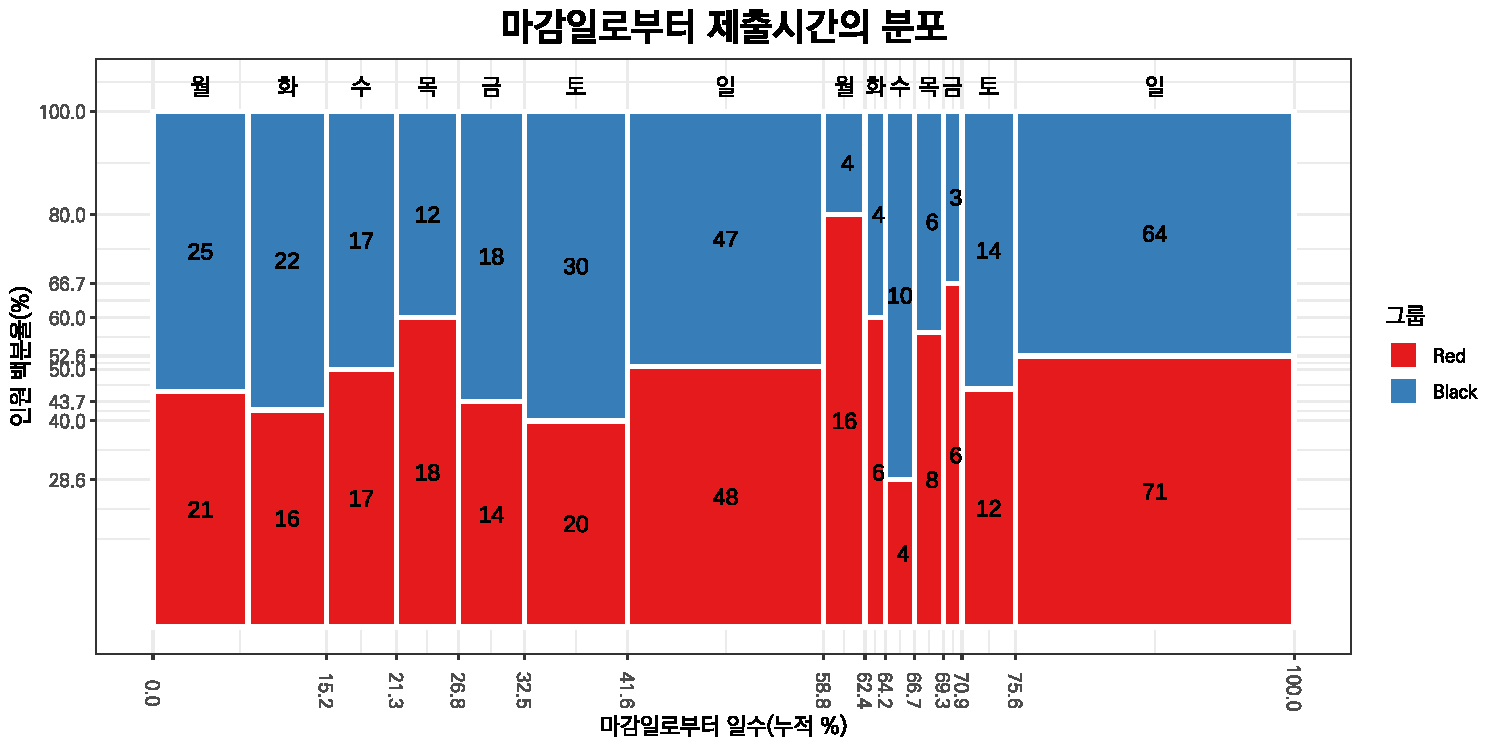
\includegraphics{_main_files/figure-latex/unnamed-chunk-77-1.pdf}

\chapter{4주차 데이터 실험 집계}\label{uxc8fcuxcc28-uxb370uxc774uxd130-uxc2e4uxd5d8-uxc9d1uxacc4-3}

\section{실험의 목적}\label{uxc2e4uxd5d8uxc758-uxbaa9uxc801-3}

4주차 구글 예습 설문지 집계결과를 분석합니다.

Q1\textasciitilde Q6에서는 랜덤화의 효과로 Red, Black 이 얼마나 닮았는지 알아봅니다.

Q7에서는 부연설명을 어느 쪽에 붙이느냐에 따라서 Red 와 Black 의 응답이 달라지는 것을 알아봅니다.

끝으로 제출시간의 분포가 날마다 고른지, Red, Black 간에는 닮았는지 알아봅니다.

\subsection{Red, Black을 잘못 표시한 사람들}\label{red-blackuxc744-uxc798uxbabb-uxd45cuxc2dcuxd55c-uxc0acuxb78cuxb4e4-3}

\begin{longtable}[]{@{}
  >{\raggedright\arraybackslash}p{(\columnwidth - 4\tabcolsep) * \real{0.3611}}
  >{\centering\arraybackslash}p{(\columnwidth - 4\tabcolsep) * \real{0.2778}}
  >{\centering\arraybackslash}p{(\columnwidth - 4\tabcolsep) * \real{0.3056}}@{}}
\toprule\noalign{}
\begin{minipage}[b]{\linewidth}\raggedright
~
\end{minipage} & \begin{minipage}[b]{\linewidth}\centering
Red(구글예습퀴즈)
\end{minipage} & \begin{minipage}[b]{\linewidth}\centering
Black(구글예습퀴즈)
\end{minipage} \\
\midrule\noalign{}
\endhead
\bottomrule\noalign{}
\endlastfoot
\textbf{Red(랜덤화출석부)} & 275 & 1 \\
\textbf{Black(랜덤화출석부)} & 3 & 285 \\
\textbf{계} & 278 & 286 \\
\end{longtable}

랜덤화출석부에 있는 Red, Black 과 실제 구글설문에 올린 Red, Black 이 다른 사람들의 수효는 4명입니다.

Red를 Black 이라고 한 사람이 1명, Black 을 Red 라고 한 사람이 3명입니다.

두 가지 방법으로 분석합니다.

우선 Red, Black 을 잘못 선택한 4명을 랜덤하게 둘로 나누면 어느 한 쪽 집단에 들어갈 기대인원은 4명을 둘로 나눈 2(명)이고, 표준오차는 4의 제곱근에 1/2을 곱해 준 1명이 됩니다.

실제로 Red를 Black 이라고 한 사람수, 1명이나 Black 을 Red 라고 한 사람수, 3명은 기대인원으로부터 표준오차 범위, 혹은 표준오차 두 배 범위에는 잘 들어갑니다.

두 번째 분석 방법은 확률을 계산해 보는 것입니다.

Red, Black 을 잘못 선택한 4명을 랜덤하게 둘로 나눌 때, 실제로 관찰된 3명 이상이나 1명이하로 잘못 선택한 사람수가 나올 가능성은 얼마나 되는가 입니다.

이 경우 공평한 동전던지기를 확률 법칙으로 표현한 이항분포로부터 계산할 수 있습니다.

시행횟수가 4이고 한 번 시행에서 성공확률이 1/2 인 이항분포에서 성공횟수가 1이하이거나 3이상을 관찰할 확률은 0.625입니다.

공평한 동전 던지기에서 앞면이 1개 이하 나오는 확률은 3개 이상 나오는 확률과 같기 때문에 사실상 한쪽만 계산해서 2배 해 주면 됩니다.

이 값을 p-value 라고 하는데, p-value가 0.05보다 작을 때 \textbf{통계적으로 유의한 차이를 관찰}하였다고 말합니다.

즉, 공평한 동전을 던지는 것과 같은 과정이라고 가정하였을 때 실제로 관찰된 값들이 가정으로부터 얼마나 떨어져 있는지를 표현한 것입니다.

0.05는 이런 실험을 스무 번 정도 반복하면 1번 나올 정도로 드문 사건을 의미합니다.

즉 가정이 잘못되었다는 것입니다.

그런데 Red, Black 을 잘못 표시한 사람들의 분포에서 관찰된 p-value 는 0.05와는 비교도 안될 정도로 큰 값입니다.

따라서 두 집단이 랜덤화 효과가 작동하여 \textbf{통계적으로 유의한 차이를 보이지 않는다}고 할 수 있습니다.

\subsection{응답인원의 Red, Black}\label{uxc751uxb2f5uxc778uxc6d0uxc758-red-black-3}

Red 로 응답한 인원은 278명, Black 에 응답한 인원은 286명입니다.

전체 응답인원 564 명을 랜덤하게 둘로 나눌 때 어느 한 쪽의 기대인원은 전체 응답인원의 절반인 282명이고, 표준오차는 전체 응답인원의 제곱근에 1/2을 곱해 준 11.9 명입니다.

따라서 Red, Black 각 그룹에 관찰된 인원은 기대인원으로부터 표준오차 범위, 혹은 2배의 표준오차 범위 안에 들어갑니다.

\section{Q1. 세종대왕 시대 조세제도}\label{q1.-uxc138uxc885uxb300uxc655-uxc2dcuxb300-uxc870uxc138uxc81cuxb3c4}

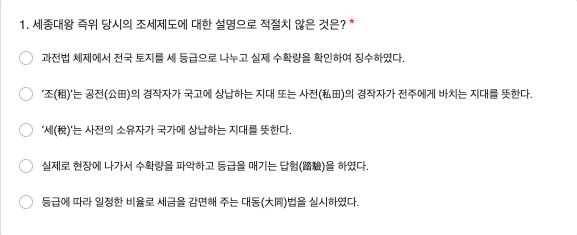
\includegraphics[width=0.75\linewidth]{./pics/Quiz230322_Q1}

\subsection{조선초기 조세제도}\label{uxc870uxc120uxcd08uxae30-uxc870uxc138uxc81cuxb3c4}

\begin{longtable}[]{@{}
  >{\raggedright\arraybackslash}p{(\columnwidth - 12\tabcolsep) * \real{0.0674}}
  >{\centering\arraybackslash}p{(\columnwidth - 12\tabcolsep) * \real{0.1854}}
  >{\centering\arraybackslash}p{(\columnwidth - 12\tabcolsep) * \real{0.1854}}
  >{\centering\arraybackslash}p{(\columnwidth - 12\tabcolsep) * \real{0.1854}}
  >{\centering\arraybackslash}p{(\columnwidth - 12\tabcolsep) * \real{0.1798}}
  >{\centering\arraybackslash}p{(\columnwidth - 12\tabcolsep) * \real{0.1629}}
  >{\centering\arraybackslash}p{(\columnwidth - 12\tabcolsep) * \real{0.0337}}@{}}
\toprule\noalign{}
\begin{minipage}[b]{\linewidth}\raggedright
~
\end{minipage} & \begin{minipage}[b]{\linewidth}\centering
과전법 체제에서 전국 토지를 세
등급으로 나누고 실제 수확량을
확인하여 징수하였다.
\end{minipage} & \begin{minipage}[b]{\linewidth}\centering
'조(租)'는 공전(公田)의
경작자가 국고에 상납하는 지대
또는 사전(私田)의 경작자가
전주에게 바치는 지대를 뜻한다.
\end{minipage} & \begin{minipage}[b]{\linewidth}\centering
'세(稅)'는 사전의 소유자가
국가에 상납하는 지세를 뜻한다.
\end{minipage} & \begin{minipage}[b]{\linewidth}\centering
실제로 현장에 나가서 수확량을
파악하고 등급을 매기는
답험(踏驗)을 하였다.
\end{minipage} & \begin{minipage}[b]{\linewidth}\centering
등급에 따라 일정한 비율로
세금을 감면해 주는
대동(大同)법을 실시하였다.
\end{minipage} & \begin{minipage}[b]{\linewidth}\centering
계
\end{minipage} \\
\midrule\noalign{}
\endhead
\bottomrule\noalign{}
\endlastfoot
\textbf{Red} & 22 & 28 & 26 & 22 & 180 & 278 \\
\textbf{Black} & 17 & 30 & 17 & 19 & 203 & 286 \\
\textbf{계} & 39 & 58 & 43 & 41 & 383 & 564 \\
\end{longtable}

\begin{longtable}[]{@{}
  >{\raggedleft\arraybackslash}p{(\columnwidth - 4\tabcolsep) * \real{0.2361}}
  >{\raggedleft\arraybackslash}p{(\columnwidth - 4\tabcolsep) * \real{0.0694}}
  >{\raggedleft\arraybackslash}p{(\columnwidth - 4\tabcolsep) * \real{0.1389}}@{}}
\caption{Pearson's Chi-squared test: \texttt{.}}\tabularnewline
\toprule\noalign{}
\begin{minipage}[b]{\linewidth}\raggedleft
Test statistic
\end{minipage} & \begin{minipage}[b]{\linewidth}\raggedleft
df
\end{minipage} & \begin{minipage}[b]{\linewidth}\raggedleft
P value
\end{minipage} \\
\midrule\noalign{}
\endfirsthead
\toprule\noalign{}
\begin{minipage}[b]{\linewidth}\raggedleft
Test statistic
\end{minipage} & \begin{minipage}[b]{\linewidth}\raggedleft
df
\end{minipage} & \begin{minipage}[b]{\linewidth}\raggedleft
P value
\end{minipage} \\
\midrule\noalign{}
\endhead
\bottomrule\noalign{}
\endlastfoot
4.082 & 4 & 0.3951 \\
\end{longtable}

Q1의 집계 결과가 Red, Black 간에 통계적으로 유의한 차이가 있는지 알아보기 위하여 카이제곱 테스트를 수행하였습니다.

그 결과 카이제곱 통계량은 4.08, 자유도는 4 , p-value 는 0.3951이므로 Red, Black 간에 통계적으로 유의한 차이를 보이지 않습니다.

실제로 닮은 게 느껴집니까?

\subsection{조선초기 조세제도(\%)}\label{uxc870uxc120uxcd08uxae30-uxc870uxc138uxc81cuxb3c4-1}

\begin{longtable}[]{@{}
  >{\centering\arraybackslash}p{(\columnwidth - 10\tabcolsep) * \real{0.1964}}
  >{\centering\arraybackslash}p{(\columnwidth - 10\tabcolsep) * \real{0.1964}}
  >{\centering\arraybackslash}p{(\columnwidth - 10\tabcolsep) * \real{0.1964}}
  >{\centering\arraybackslash}p{(\columnwidth - 10\tabcolsep) * \real{0.1905}}
  >{\centering\arraybackslash}p{(\columnwidth - 10\tabcolsep) * \real{0.1726}}
  >{\centering\arraybackslash}p{(\columnwidth - 10\tabcolsep) * \real{0.0476}}@{}}
\toprule\noalign{}
\begin{minipage}[b]{\linewidth}\centering
과전법 체제에서 전국 토지를 세
등급으로 나누고 실제 수확량을
확인하여 징수하였다.
\end{minipage} & \begin{minipage}[b]{\linewidth}\centering
'조(租)'는 공전(公田)의
경작자가 국고에 상납하는 지대
또는 사전(私田)의 경작자가
전주에게 바치는 지대를 뜻한다.
\end{minipage} & \begin{minipage}[b]{\linewidth}\centering
'세(稅)'는 사전의 소유자가
국가에 상납하는 지세를 뜻한다.
\end{minipage} & \begin{minipage}[b]{\linewidth}\centering
실제로 현장에 나가서 수확량을
파악하고 등급을 매기는
답험(踏驗)을 하였다.
\end{minipage} & \begin{minipage}[b]{\linewidth}\centering
등급에 따라 일정한 비율로
세금을 감면해 주는
대동(大同)법을 실시하였다.
\end{minipage} & \begin{minipage}[b]{\linewidth}\centering
계
\end{minipage} \\
\midrule\noalign{}
\endhead
\bottomrule\noalign{}
\endlastfoot
6.9 & 10.3 & 7.6 & 7.3 & 67.9 & 100.0 \\
\end{longtable}

정답률은 Red, Black 을 합하여 계산하는데, 67.9(\%) 입니다.

\section{Q2. 공법도입에 대한 대신들의 찬성율}\label{q2.-uxacf5uxbc95uxb3c4uxc785uxc5d0-uxb300uxd55c-uxb300uxc2e0uxb4e4uxc758-uxcc2cuxc131uxc728}

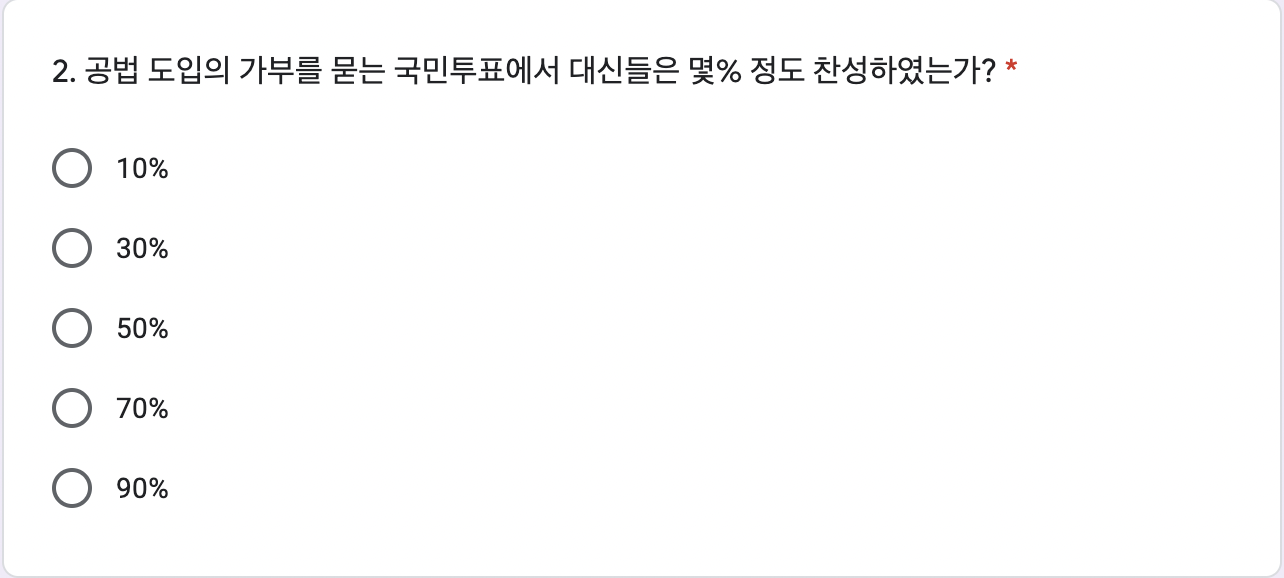
\includegraphics[width=0.75\linewidth]{./pics/Quiz210913_Q2}

\subsection{공법도입과 대신들(집계표)}\label{uxacf5uxbc95uxb3c4uxc785uxacfc-uxb300uxc2e0uxb4e4uxc9d1uxacc4uxd45c}

\begin{longtable}[]{@{}
  >{\raggedright\arraybackslash}p{(\columnwidth - 12\tabcolsep) * \real{0.1667}}
  >{\raggedleft\arraybackslash}p{(\columnwidth - 12\tabcolsep) * \real{0.0833}}
  >{\raggedleft\arraybackslash}p{(\columnwidth - 12\tabcolsep) * \real{0.0833}}
  >{\raggedleft\arraybackslash}p{(\columnwidth - 12\tabcolsep) * \real{0.0833}}
  >{\raggedleft\arraybackslash}p{(\columnwidth - 12\tabcolsep) * \real{0.0833}}
  >{\raggedleft\arraybackslash}p{(\columnwidth - 12\tabcolsep) * \real{0.0833}}
  >{\centering\arraybackslash}p{(\columnwidth - 12\tabcolsep) * \real{0.0833}}@{}}
\toprule\noalign{}
\begin{minipage}[b]{\linewidth}\raggedright
~
\end{minipage} & \begin{minipage}[b]{\linewidth}\raggedleft
10\%
\end{minipage} & \begin{minipage}[b]{\linewidth}\raggedleft
30\%
\end{minipage} & \begin{minipage}[b]{\linewidth}\raggedleft
50\%
\end{minipage} & \begin{minipage}[b]{\linewidth}\raggedleft
70\%
\end{minipage} & \begin{minipage}[b]{\linewidth}\raggedleft
90\%
\end{minipage} & \begin{minipage}[b]{\linewidth}\centering
계
\end{minipage} \\
\midrule\noalign{}
\endhead
\bottomrule\noalign{}
\endlastfoot
\textbf{Red} & 153 & 54 & 28 & 27 & 16 & 278 \\
\textbf{Black} & 160 & 46 & 26 & 32 & 22 & 286 \\
\textbf{계} & 313 & 100 & 54 & 59 & 38 & 564 \\
\end{longtable}

\begin{longtable}[]{@{}
  >{\raggedleft\arraybackslash}p{(\columnwidth - 4\tabcolsep) * \real{0.2361}}
  >{\raggedleft\arraybackslash}p{(\columnwidth - 4\tabcolsep) * \real{0.0694}}
  >{\raggedleft\arraybackslash}p{(\columnwidth - 4\tabcolsep) * \real{0.1389}}@{}}
\caption{Pearson's Chi-squared test: \texttt{.}}\tabularnewline
\toprule\noalign{}
\begin{minipage}[b]{\linewidth}\raggedleft
Test statistic
\end{minipage} & \begin{minipage}[b]{\linewidth}\raggedleft
df
\end{minipage} & \begin{minipage}[b]{\linewidth}\raggedleft
P value
\end{minipage} \\
\midrule\noalign{}
\endfirsthead
\toprule\noalign{}
\begin{minipage}[b]{\linewidth}\raggedleft
Test statistic
\end{minipage} & \begin{minipage}[b]{\linewidth}\raggedleft
df
\end{minipage} & \begin{minipage}[b]{\linewidth}\raggedleft
P value
\end{minipage} \\
\midrule\noalign{}
\endhead
\bottomrule\noalign{}
\endlastfoot
2.129 & 4 & 0.7121 \\
\end{longtable}

Q2의 집계 결과가 Red, Black 간에 통계적으로 유의한 차이가 있는지 알아보기 위하여 카이제곱 테스트를 수행하였습니다.

그 결과 카이제곱 통계량은 2.129, 자유도는 4, p-value 는 0.7121이므로 Red, Black 간에 통계적으로 유의한 차이를 보이지 않습니다.

실제로 닮은 게 느껴집니까?

\subsection{공법도입과 대신들(\%)}\label{uxacf5uxbc95uxb3c4uxc785uxacfc-uxb300uxc2e0uxb4e4}

\begin{longtable}[]{@{}
  >{\raggedleft\arraybackslash}p{(\columnwidth - 10\tabcolsep) * \real{0.0972}}
  >{\raggedleft\arraybackslash}p{(\columnwidth - 10\tabcolsep) * \real{0.0972}}
  >{\raggedleft\arraybackslash}p{(\columnwidth - 10\tabcolsep) * \real{0.0833}}
  >{\raggedleft\arraybackslash}p{(\columnwidth - 10\tabcolsep) * \real{0.0972}}
  >{\raggedleft\arraybackslash}p{(\columnwidth - 10\tabcolsep) * \real{0.0833}}
  >{\centering\arraybackslash}p{(\columnwidth - 10\tabcolsep) * \real{0.1111}}@{}}
\toprule\noalign{}
\begin{minipage}[b]{\linewidth}\raggedleft
10\%
\end{minipage} & \begin{minipage}[b]{\linewidth}\raggedleft
30\%
\end{minipage} & \begin{minipage}[b]{\linewidth}\raggedleft
50\%
\end{minipage} & \begin{minipage}[b]{\linewidth}\raggedleft
70\%
\end{minipage} & \begin{minipage}[b]{\linewidth}\raggedleft
90\%
\end{minipage} & \begin{minipage}[b]{\linewidth}\centering
계
\end{minipage} \\
\midrule\noalign{}
\endhead
\bottomrule\noalign{}
\endlastfoot
55.5 & 17.7 & 9.6 & 10.5 & 6.7 & 100.0 \\
\end{longtable}

정답률은 Red, Black 을 합하여 계산하는데, 55.5(\%) 입니다.

\section{Q3. 공법도입과 품관촌민들의 찬반}\label{q3.-uxacf5uxbc95uxb3c4uxc785uxacfc-uxd488uxad00uxcd0cuxbbfcuxb4e4uxc758-uxcc2cuxbc18}

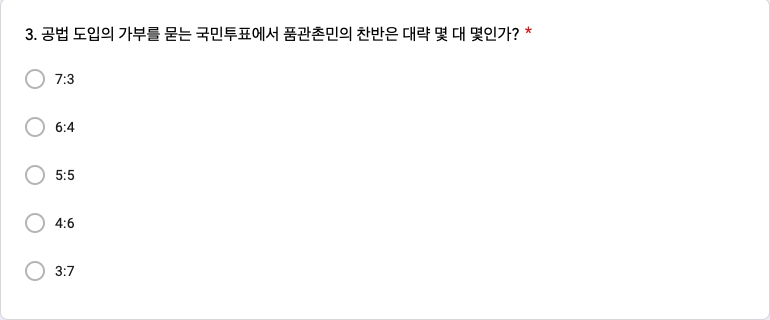
\includegraphics[width=0.75\linewidth]{./pics/Quiz210316_Q3}

\subsection{품관촌민들의 찬반(집계표)}\label{uxd488uxad00uxcd0cuxbbfcuxb4e4uxc758-uxcc2cuxbc18uxc9d1uxacc4uxd45c}

\begin{longtable}[]{@{}
  >{\raggedright\arraybackslash}p{(\columnwidth - 12\tabcolsep) * \real{0.1667}}
  >{\raggedleft\arraybackslash}p{(\columnwidth - 12\tabcolsep) * \real{0.0833}}
  >{\raggedleft\arraybackslash}p{(\columnwidth - 12\tabcolsep) * \real{0.0833}}
  >{\raggedleft\arraybackslash}p{(\columnwidth - 12\tabcolsep) * \real{0.0833}}
  >{\raggedleft\arraybackslash}p{(\columnwidth - 12\tabcolsep) * \real{0.0833}}
  >{\raggedleft\arraybackslash}p{(\columnwidth - 12\tabcolsep) * \real{0.0833}}
  >{\centering\arraybackslash}p{(\columnwidth - 12\tabcolsep) * \real{0.0833}}@{}}
\toprule\noalign{}
\begin{minipage}[b]{\linewidth}\raggedright
~
\end{minipage} & \begin{minipage}[b]{\linewidth}\raggedleft
7:3
\end{minipage} & \begin{minipage}[b]{\linewidth}\raggedleft
6:4
\end{minipage} & \begin{minipage}[b]{\linewidth}\raggedleft
5:5
\end{minipage} & \begin{minipage}[b]{\linewidth}\raggedleft
4:6
\end{minipage} & \begin{minipage}[b]{\linewidth}\raggedleft
3:7
\end{minipage} & \begin{minipage}[b]{\linewidth}\centering
계
\end{minipage} \\
\midrule\noalign{}
\endhead
\bottomrule\noalign{}
\endlastfoot
\textbf{Red} & 48 & 159 & 25 & 22 & 24 & 278 \\
\textbf{Black} & 62 & 162 & 25 & 18 & 19 & 286 \\
\textbf{계} & 110 & 321 & 50 & 40 & 43 & 564 \\
\end{longtable}

\begin{longtable}[]{@{}
  >{\raggedleft\arraybackslash}p{(\columnwidth - 4\tabcolsep) * \real{0.2361}}
  >{\raggedleft\arraybackslash}p{(\columnwidth - 4\tabcolsep) * \real{0.0694}}
  >{\raggedleft\arraybackslash}p{(\columnwidth - 4\tabcolsep) * \real{0.1389}}@{}}
\caption{Pearson's Chi-squared test: \texttt{.}}\tabularnewline
\toprule\noalign{}
\begin{minipage}[b]{\linewidth}\raggedleft
Test statistic
\end{minipage} & \begin{minipage}[b]{\linewidth}\raggedleft
df
\end{minipage} & \begin{minipage}[b]{\linewidth}\raggedleft
P value
\end{minipage} \\
\midrule\noalign{}
\endfirsthead
\toprule\noalign{}
\begin{minipage}[b]{\linewidth}\raggedleft
Test statistic
\end{minipage} & \begin{minipage}[b]{\linewidth}\raggedleft
df
\end{minipage} & \begin{minipage}[b]{\linewidth}\raggedleft
P value
\end{minipage} \\
\midrule\noalign{}
\endhead
\bottomrule\noalign{}
\endlastfoot
2.678 & 4 & 0.613 \\
\end{longtable}

Q3의 집계 결과가 Red, Black 간에 통계적으로 유의한 차이가 있는지 알아보기 위하여 카이제곱 테스트를 수행하였습니다.

그 결과 카이제곱 통계량은 2.678, 자유도는 4, p-value 는 0.6130이므로 Red, Black 간에 통계적으로 유의한 차이를 보이지 않습니다.

실제로 닮은 게 느껴집니까?

\subsection{품관촌민들의 찬반(\%)}\label{uxd488uxad00uxcd0cuxbbfcuxb4e4uxc758-uxcc2cuxbc18}

\begin{longtable}[]{@{}
  >{\raggedleft\arraybackslash}p{(\columnwidth - 10\tabcolsep) * \real{0.0972}}
  >{\raggedleft\arraybackslash}p{(\columnwidth - 10\tabcolsep) * \real{0.0972}}
  >{\raggedleft\arraybackslash}p{(\columnwidth - 10\tabcolsep) * \real{0.0833}}
  >{\raggedleft\arraybackslash}p{(\columnwidth - 10\tabcolsep) * \real{0.0833}}
  >{\raggedleft\arraybackslash}p{(\columnwidth - 10\tabcolsep) * \real{0.0833}}
  >{\centering\arraybackslash}p{(\columnwidth - 10\tabcolsep) * \real{0.1111}}@{}}
\toprule\noalign{}
\begin{minipage}[b]{\linewidth}\raggedleft
7:3
\end{minipage} & \begin{minipage}[b]{\linewidth}\raggedleft
6:4
\end{minipage} & \begin{minipage}[b]{\linewidth}\raggedleft
5:5
\end{minipage} & \begin{minipage}[b]{\linewidth}\raggedleft
4:6
\end{minipage} & \begin{minipage}[b]{\linewidth}\raggedleft
3:7
\end{minipage} & \begin{minipage}[b]{\linewidth}\centering
계
\end{minipage} \\
\midrule\noalign{}
\endhead
\bottomrule\noalign{}
\endlastfoot
19.5 & 56.9 & 8.9 & 7.1 & 7.6 & 100.0 \\
\end{longtable}

정답률은 Red, Black 을 합하여 계산하는데, 56.9(\%) 입니다.

\section{Q4. 공법}\label{q4.-uxacf5uxbc95}

\begin{flushleft}
\includegraphics[width=0.75\linewidth]{./pics/Quiz210316_Q4} \end{flushleft}

\subsection{기본세율}\label{uxae30uxbcf8uxc138uxc728}

\begin{longtable}[]{@{}
  >{\raggedright\arraybackslash}p{(\columnwidth - 10\tabcolsep) * \real{0.1667}}
  >{\raggedleft\arraybackslash}p{(\columnwidth - 10\tabcolsep) * \real{0.0972}}
  >{\raggedleft\arraybackslash}p{(\columnwidth - 10\tabcolsep) * \real{0.0972}}
  >{\raggedleft\arraybackslash}p{(\columnwidth - 10\tabcolsep) * \real{0.0972}}
  >{\raggedleft\arraybackslash}p{(\columnwidth - 10\tabcolsep) * \real{0.0972}}
  >{\centering\arraybackslash}p{(\columnwidth - 10\tabcolsep) * \real{0.0972}}@{}}
\toprule\noalign{}
\begin{minipage}[b]{\linewidth}\raggedright
~
\end{minipage} & \begin{minipage}[b]{\linewidth}\raggedleft
1/10
\end{minipage} & \begin{minipage}[b]{\linewidth}\raggedleft
1/15
\end{minipage} & \begin{minipage}[b]{\linewidth}\raggedleft
1/20
\end{minipage} & \begin{minipage}[b]{\linewidth}\raggedleft
1/30
\end{minipage} & \begin{minipage}[b]{\linewidth}\centering
계
\end{minipage} \\
\midrule\noalign{}
\endhead
\bottomrule\noalign{}
\endlastfoot
\textbf{Red} & 84 & 47 & 132 & 15 & 278 \\
\textbf{Black} & 88 & 29 & 154 & 15 & 286 \\
\textbf{계} & 172 & 76 & 286 & 30 & 564 \\
\end{longtable}

\begin{longtable}[]{@{}
  >{\raggedleft\arraybackslash}p{(\columnwidth - 4\tabcolsep) * \real{0.2361}}
  >{\raggedleft\arraybackslash}p{(\columnwidth - 4\tabcolsep) * \real{0.0694}}
  >{\raggedleft\arraybackslash}p{(\columnwidth - 4\tabcolsep) * \real{0.1389}}@{}}
\caption{Pearson's Chi-squared test: \texttt{.}}\tabularnewline
\toprule\noalign{}
\begin{minipage}[b]{\linewidth}\raggedleft
Test statistic
\end{minipage} & \begin{minipage}[b]{\linewidth}\raggedleft
df
\end{minipage} & \begin{minipage}[b]{\linewidth}\raggedleft
P value
\end{minipage} \\
\midrule\noalign{}
\endfirsthead
\toprule\noalign{}
\begin{minipage}[b]{\linewidth}\raggedleft
Test statistic
\end{minipage} & \begin{minipage}[b]{\linewidth}\raggedleft
df
\end{minipage} & \begin{minipage}[b]{\linewidth}\raggedleft
P value
\end{minipage} \\
\midrule\noalign{}
\endhead
\bottomrule\noalign{}
\endlastfoot
5.936 & 3 & 0.1148 \\
\end{longtable}

Q4의 집계 결과가 Red, Black 간에 통계적으로 유의한 차이가 있는지 알아보기 위하여 카이제곱 테스트를 수행하였습니다.

그 결과 카이제곱 통계량은 5.936, 자유도는 3, p-value 는 0.1148이므로 Red, Black 간에 통계적으로 유의한 차이를 보이지 않습니다.

실제로 닮은 게 느껴집니까?

\subsection{기본세율(\%)}\label{uxae30uxbcf8uxc138uxc728-1}

\begin{longtable}[]{@{}
  >{\raggedleft\arraybackslash}p{(\columnwidth - 8\tabcolsep) * \real{0.0972}}
  >{\raggedleft\arraybackslash}p{(\columnwidth - 8\tabcolsep) * \real{0.0972}}
  >{\raggedleft\arraybackslash}p{(\columnwidth - 8\tabcolsep) * \real{0.0972}}
  >{\raggedleft\arraybackslash}p{(\columnwidth - 8\tabcolsep) * \real{0.0972}}
  >{\centering\arraybackslash}p{(\columnwidth - 8\tabcolsep) * \real{0.1111}}@{}}
\toprule\noalign{}
\begin{minipage}[b]{\linewidth}\raggedleft
1/10
\end{minipage} & \begin{minipage}[b]{\linewidth}\raggedleft
1/15
\end{minipage} & \begin{minipage}[b]{\linewidth}\raggedleft
1/20
\end{minipage} & \begin{minipage}[b]{\linewidth}\raggedleft
1/30
\end{minipage} & \begin{minipage}[b]{\linewidth}\centering
계
\end{minipage} \\
\midrule\noalign{}
\endhead
\bottomrule\noalign{}
\endlastfoot
30.5 & 13.5 & 50.7 & 5.3 & 100.0 \\
\end{longtable}

정답률은 Red, Black 을 합하여 계산하는데, 30.5(\%) 입니다.

\section{Q5. 1423년 조선시대 호구와 인구}\label{q5.-1423uxb144-uxc870uxc120uxc2dcuxb300-uxd638uxad6cuxc640-uxc778uxad6c}

\begin{flushleft}
\includegraphics[width=0.75\linewidth]{./pics/Quiz210316_Q5} \end{flushleft}

\subsection{호구와 인구}\label{uxd638uxad6cuxc640-uxc778uxad6c}

\begin{longtable}[]{@{}
  >{\raggedright\arraybackslash}p{(\columnwidth - 10\tabcolsep) * \real{0.1667}}
  >{\centering\arraybackslash}p{(\columnwidth - 10\tabcolsep) * \real{0.1250}}
  >{\centering\arraybackslash}p{(\columnwidth - 10\tabcolsep) * \real{0.1250}}
  >{\centering\arraybackslash}p{(\columnwidth - 10\tabcolsep) * \real{0.1250}}
  >{\centering\arraybackslash}p{(\columnwidth - 10\tabcolsep) * \real{0.1389}}
  >{\centering\arraybackslash}p{(\columnwidth - 10\tabcolsep) * \real{0.0833}}@{}}
\toprule\noalign{}
\begin{minipage}[b]{\linewidth}\raggedright
~
\end{minipage} & \begin{minipage}[b]{\linewidth}\centering
15만호
\end{minipage} & \begin{minipage}[b]{\linewidth}\centering
20만호
\end{minipage} & \begin{minipage}[b]{\linewidth}\centering
44만호
\end{minipage} & \begin{minipage}[b]{\linewidth}\centering
130만호
\end{minipage} & \begin{minipage}[b]{\linewidth}\centering
계
\end{minipage} \\
\midrule\noalign{}
\endhead
\bottomrule\noalign{}
\endlastfoot
\textbf{Red} & 11 & 164 & 87 & 16 & 278 \\
\textbf{Black} & 22 & 151 & 105 & 8 & 286 \\
\textbf{계} & 33 & 315 & 192 & 24 & 564 \\
\end{longtable}

\begin{longtable}[]{@{}
  >{\raggedleft\arraybackslash}p{(\columnwidth - 4\tabcolsep) * \real{0.2361}}
  >{\raggedleft\arraybackslash}p{(\columnwidth - 4\tabcolsep) * \real{0.0694}}
  >{\raggedleft\arraybackslash}p{(\columnwidth - 4\tabcolsep) * \real{0.1667}}@{}}
\caption{Pearson's Chi-squared test: \texttt{.}}\tabularnewline
\toprule\noalign{}
\begin{minipage}[b]{\linewidth}\raggedleft
Test statistic
\end{minipage} & \begin{minipage}[b]{\linewidth}\raggedleft
df
\end{minipage} & \begin{minipage}[b]{\linewidth}\raggedleft
P value
\end{minipage} \\
\midrule\noalign{}
\endfirsthead
\toprule\noalign{}
\begin{minipage}[b]{\linewidth}\raggedleft
Test statistic
\end{minipage} & \begin{minipage}[b]{\linewidth}\raggedleft
df
\end{minipage} & \begin{minipage}[b]{\linewidth}\raggedleft
P value
\end{minipage} \\
\midrule\noalign{}
\endhead
\bottomrule\noalign{}
\endlastfoot
8.446 & 3 & 0.03765 * \\
\end{longtable}

Q5의 집계 결과가 Red, Black 간에 통계적으로 유의한 차이가 있는지 알아보기 위하여 카이제곱 테스트를 수행하였습니다.

그 결과 카이제곱 통계량은 8.446, 자유도는 3, p-value 는 0.0376이므로 Red, Black 간에 통계적으로 유의한 차이를 보이고 있습니다.

\subsection{호구와 인구(\%)}\label{uxd638uxad6cuxc640-uxc778uxad6c-1}

\begin{longtable}[]{@{}
  >{\centering\arraybackslash}p{(\columnwidth - 8\tabcolsep) * \real{0.1250}}
  >{\centering\arraybackslash}p{(\columnwidth - 8\tabcolsep) * \real{0.1250}}
  >{\centering\arraybackslash}p{(\columnwidth - 8\tabcolsep) * \real{0.1250}}
  >{\centering\arraybackslash}p{(\columnwidth - 8\tabcolsep) * \real{0.1389}}
  >{\centering\arraybackslash}p{(\columnwidth - 8\tabcolsep) * \real{0.1389}}@{}}
\toprule\noalign{}
\begin{minipage}[b]{\linewidth}\centering
15만호
\end{minipage} & \begin{minipage}[b]{\linewidth}\centering
20만호
\end{minipage} & \begin{minipage}[b]{\linewidth}\centering
44만호
\end{minipage} & \begin{minipage}[b]{\linewidth}\centering
130만호
\end{minipage} & \begin{minipage}[b]{\linewidth}\centering
계
\end{minipage} \\
\midrule\noalign{}
\endhead
\bottomrule\noalign{}
\endlastfoot
5.9 & 55.9 & 34.0 & 4.3 & 100.0 \\
\end{longtable}

정답률은 Red, Black 을 합하여 계산하는데, 55.9(\%) 입니다.

\section{Q6. 지방관료와 품관촌민}\label{q6.-uxc9c0uxbc29uxad00uxb8ccuxc640-uxd488uxad00uxcd0cuxbbfc}

\begin{flushleft}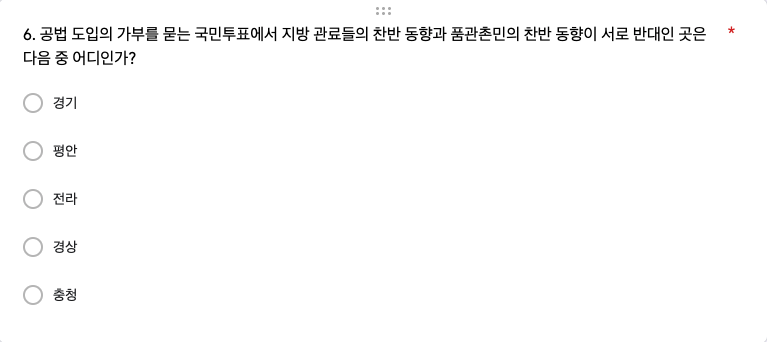
\includegraphics[width=0.75\linewidth]{./pics/Quiz210316_Q6} \end{flushleft}

\subsection{찬반이 반대인 곳(집계표)}\label{uxcc2cuxbc18uxc774-uxbc18uxb300uxc778-uxacf3uxc9d1uxacc4uxd45c}

\begin{longtable}[]{@{}
  >{\raggedright\arraybackslash}p{(\columnwidth - 12\tabcolsep) * \real{0.1667}}
  >{\centering\arraybackslash}p{(\columnwidth - 12\tabcolsep) * \real{0.0972}}
  >{\centering\arraybackslash}p{(\columnwidth - 12\tabcolsep) * \real{0.0972}}
  >{\centering\arraybackslash}p{(\columnwidth - 12\tabcolsep) * \real{0.0972}}
  >{\centering\arraybackslash}p{(\columnwidth - 12\tabcolsep) * \real{0.0972}}
  >{\centering\arraybackslash}p{(\columnwidth - 12\tabcolsep) * \real{0.0972}}
  >{\centering\arraybackslash}p{(\columnwidth - 12\tabcolsep) * \real{0.0972}}@{}}
\toprule\noalign{}
\begin{minipage}[b]{\linewidth}\raggedright
~
\end{minipage} & \begin{minipage}[b]{\linewidth}\centering
경기
\end{minipage} & \begin{minipage}[b]{\linewidth}\centering
평안
\end{minipage} & \begin{minipage}[b]{\linewidth}\centering
전라
\end{minipage} & \begin{minipage}[b]{\linewidth}\centering
경상
\end{minipage} & \begin{minipage}[b]{\linewidth}\centering
충청
\end{minipage} & \begin{minipage}[b]{\linewidth}\centering
계
\end{minipage} \\
\midrule\noalign{}
\endhead
\bottomrule\noalign{}
\endlastfoot
\textbf{Red} & 25 & 39 & 44 & 40 & 130 & 278 \\
\textbf{Black} & 25 & 37 & 51 & 43 & 130 & 286 \\
\textbf{계} & 50 & 76 & 95 & 83 & 260 & 564 \\
\end{longtable}

\begin{longtable}[]{@{}
  >{\raggedleft\arraybackslash}p{(\columnwidth - 4\tabcolsep) * \real{0.2361}}
  >{\raggedleft\arraybackslash}p{(\columnwidth - 4\tabcolsep) * \real{0.0694}}
  >{\raggedleft\arraybackslash}p{(\columnwidth - 4\tabcolsep) * \real{0.1389}}@{}}
\caption{Pearson's Chi-squared test: \texttt{.}}\tabularnewline
\toprule\noalign{}
\begin{minipage}[b]{\linewidth}\raggedleft
Test statistic
\end{minipage} & \begin{minipage}[b]{\linewidth}\raggedleft
df
\end{minipage} & \begin{minipage}[b]{\linewidth}\raggedleft
P value
\end{minipage} \\
\midrule\noalign{}
\endfirsthead
\toprule\noalign{}
\begin{minipage}[b]{\linewidth}\raggedleft
Test statistic
\end{minipage} & \begin{minipage}[b]{\linewidth}\raggedleft
df
\end{minipage} & \begin{minipage}[b]{\linewidth}\raggedleft
P value
\end{minipage} \\
\midrule\noalign{}
\endhead
\bottomrule\noalign{}
\endlastfoot
0.5635 & 4 & 0.967 \\
\end{longtable}

Q6의 집계 결과가 Red, Black 간에 통계적으로 유의한 차이가 있는지 알아보기 위하여 카이제곱 테스트를 수행하였습니다.

그 결과 카이제곱 통계량은 0.563, 자유도는 4, p-value 는 0.9670이므로 Red, Black 간에 통계적으로 유의한 차이를 보이지 않습니다.

실제로 닮은 게 느껴집니까?

\subsection{찬반이 반대인 곳(\%)}\label{uxcc2cuxbc18uxc774-uxbc18uxb300uxc778-uxacf3}

\begin{longtable}[]{@{}
  >{\centering\arraybackslash}p{(\columnwidth - 10\tabcolsep) * \real{0.0972}}
  >{\centering\arraybackslash}p{(\columnwidth - 10\tabcolsep) * \real{0.0972}}
  >{\centering\arraybackslash}p{(\columnwidth - 10\tabcolsep) * \real{0.0972}}
  >{\centering\arraybackslash}p{(\columnwidth - 10\tabcolsep) * \real{0.0972}}
  >{\centering\arraybackslash}p{(\columnwidth - 10\tabcolsep) * \real{0.0972}}
  >{\centering\arraybackslash}p{(\columnwidth - 10\tabcolsep) * \real{0.1111}}@{}}
\toprule\noalign{}
\begin{minipage}[b]{\linewidth}\centering
경기
\end{minipage} & \begin{minipage}[b]{\linewidth}\centering
평안
\end{minipage} & \begin{minipage}[b]{\linewidth}\centering
전라
\end{minipage} & \begin{minipage}[b]{\linewidth}\centering
경상
\end{minipage} & \begin{minipage}[b]{\linewidth}\centering
충청
\end{minipage} & \begin{minipage}[b]{\linewidth}\centering
계
\end{minipage} \\
\midrule\noalign{}
\endhead
\bottomrule\noalign{}
\endlastfoot
8.9 & 13.5 & 16.8 & 14.7 & 46.1 & 100.0 \\
\end{longtable}

정답률은 Red, Black 을 합하여 계산하는데, 46.1(\%) 입니다.

\section{Q7. 부연설명의 효과 : 주당 근로 69시간제 도입 찬반}\label{q7.-uxbd80uxc5f0uxc124uxba85uxc758-uxd6a8uxacfc-uxc8fcuxb2f9-uxadfcuxb85c-69uxc2dcuxac04uxc81c-uxb3c4uxc785-uxcc2cuxbc18}

부연설명을 찬성 쪽에 붙이는가(Red), 또는 반대 쪽에 붙이는가(Black)에 따라 응답이 영향을 받는 것으로 관찰됩니다.

찬반여부에 대한 카이제곱테스트의 p-value를 놓고 볼 때 그 차이가 통계적으로 매우 유의합니다.

\begin{flushleft}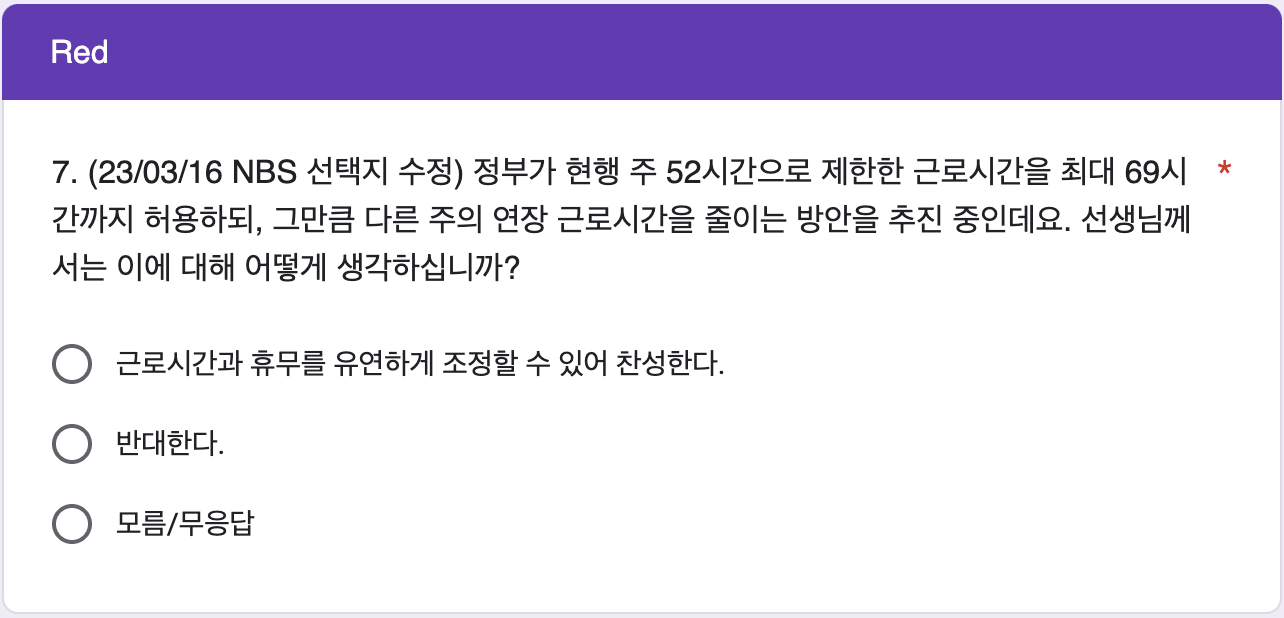
\includegraphics[width=0.67\linewidth]{./pics/Quiz240322_Q7_Red} \end{flushleft}

\begin{flushleft}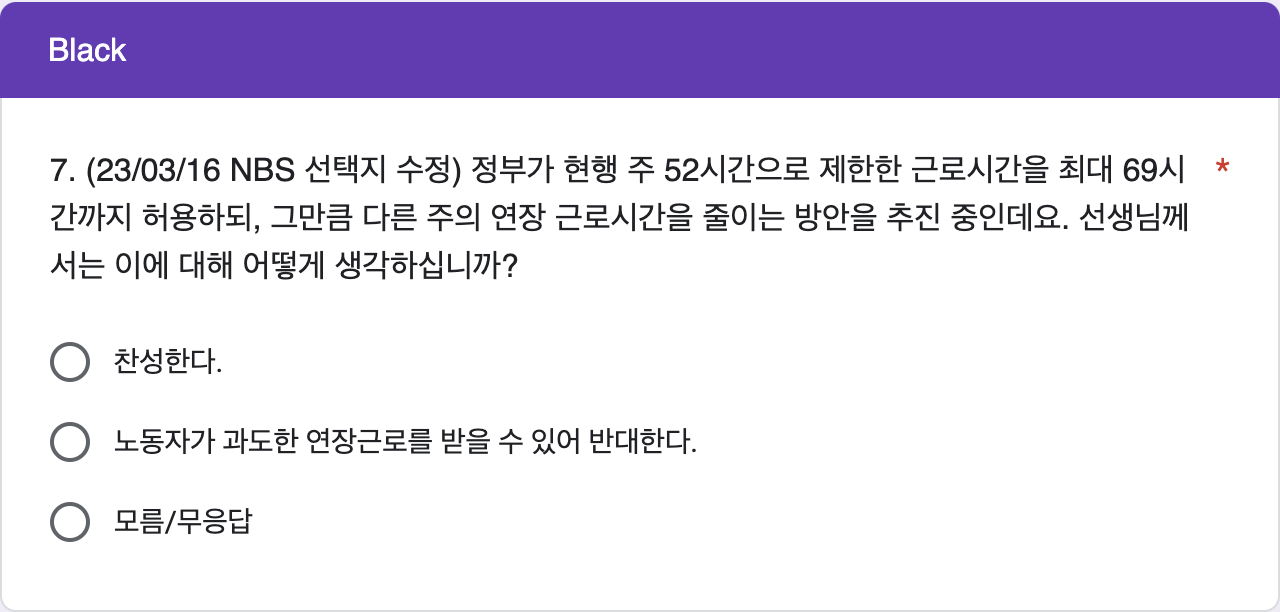
\includegraphics[width=0.67\linewidth]{./pics/Quiz240322_Q7_Black} \end{flushleft}

\subsection{집계}\label{uxc9d1uxacc4-1}

\begin{longtable}[]{@{}
  >{\raggedright\arraybackslash}p{(\columnwidth - 8\tabcolsep) * \real{0.4286}}
  >{\centering\arraybackslash}p{(\columnwidth - 8\tabcolsep) * \real{0.1558}}
  >{\centering\arraybackslash}p{(\columnwidth - 8\tabcolsep) * \real{0.1558}}
  >{\centering\arraybackslash}p{(\columnwidth - 8\tabcolsep) * \real{0.1818}}
  >{\centering\arraybackslash}p{(\columnwidth - 8\tabcolsep) * \real{0.0779}}@{}}
\toprule\noalign{}
\begin{minipage}[b]{\linewidth}\raggedright
~
\end{minipage} & \begin{minipage}[b]{\linewidth}\centering
찬성한다.
\end{minipage} & \begin{minipage}[b]{\linewidth}\centering
반대한다.
\end{minipage} & \begin{minipage}[b]{\linewidth}\centering
모름/무응답
\end{minipage} & \begin{minipage}[b]{\linewidth}\centering
계
\end{minipage} \\
\midrule\noalign{}
\endhead
\bottomrule\noalign{}
\endlastfoot
\textbf{Red(찬성한다에 부연설명)} & 132 & 78 & 68 & 278 \\
\textbf{Black(반대한다에 부연설명)} & 85 & 146 & 55 & 286 \\
\textbf{계} & 217 & 224 & 123 & 564 \\
\end{longtable}

\begin{longtable}[]{@{}
  >{\raggedleft\arraybackslash}p{(\columnwidth - 4\tabcolsep) * \real{0.2361}}
  >{\raggedleft\arraybackslash}p{(\columnwidth - 4\tabcolsep) * \real{0.0694}}
  >{\raggedleft\arraybackslash}p{(\columnwidth - 4\tabcolsep) * \real{0.2500}}@{}}
\caption{Pearson's Chi-squared test: \texttt{.}}\tabularnewline
\toprule\noalign{}
\begin{minipage}[b]{\linewidth}\raggedleft
Test statistic
\end{minipage} & \begin{minipage}[b]{\linewidth}\raggedleft
df
\end{minipage} & \begin{minipage}[b]{\linewidth}\raggedleft
P value
\end{minipage} \\
\midrule\noalign{}
\endfirsthead
\toprule\noalign{}
\begin{minipage}[b]{\linewidth}\raggedleft
Test statistic
\end{minipage} & \begin{minipage}[b]{\linewidth}\raggedleft
df
\end{minipage} & \begin{minipage}[b]{\linewidth}\raggedleft
P value
\end{minipage} \\
\midrule\noalign{}
\endhead
\bottomrule\noalign{}
\endlastfoot
32.09 & 2 & 1.076e-07 * * * \\
\end{longtable}

Q7의 Red는 주당 근로 69시간제의 도입에 찬반을 묻는 질문 중 찬성을 유도하는 부연설명을 붙였을 때 278명이 응답한 가운데 132명이 ``찬성한다''는 반응을 보이고, 78명이 ``반대한다''는 반응을 보입니다.

Black은 같은 상황에서 반대를 유도하는 부연설명을 붙였을 떄 286명이 응답한 가운데 85명이 ``찬성한다''는 반응을 보이고, 146명이 ``반대한다''는 반응을 보입니다.

그리고 ``모름/무응답''에 답한 인원은 Red에 68명, Black 에 55명이 응답하였습니다.

카이제곱 테스트는 이와 같은 상황에서
찬성을 유도하는 부연설명을 붙인 경우와 반대를 유도하는 부연설명을 붙인 경우에 그 응답의 차이가 통계적으로 유의하다는 것을 보여 줍니다.

카이제곱 통계량은 32.090, 자유도는 2, p-value 는 1.1e-07으로
부연설명을 어디에 붙이느냐에 따라 그 차이가 통계적으로 유의한 것으로 나왔습니다.

여기서 부연설명이 응답에 영향을 끼치지 않는다고 가정해 봅시다.

그렇다면 Red, Black 의 응답은 대부분의 Q1 \textasciitilde{} Q6 에서와 같이 랜덤화 효과에 의하여 통계적으로 유의한 차이를 보이지 않을 것입니다.

그런데 실제로 관찰된 카이제곱 통계값은 통계적으로 유의한 차이를 보여 주고 있습니다.

따라서 부연설명이 영향을 끼치지 않는다는 가정은 티당치 않은 것으로 볼 수밖에 없습니다.

이러한 논증 방식을 귀류법이라 합니다.

\subsection{\% 비교}\label{uxbe44uxad50-2}

\begin{longtable}[]{@{}
  >{\raggedright\arraybackslash}p{(\columnwidth - 8\tabcolsep) * \real{0.4177}}
  >{\centering\arraybackslash}p{(\columnwidth - 8\tabcolsep) * \real{0.1519}}
  >{\centering\arraybackslash}p{(\columnwidth - 8\tabcolsep) * \real{0.1519}}
  >{\centering\arraybackslash}p{(\columnwidth - 8\tabcolsep) * \real{0.1772}}
  >{\centering\arraybackslash}p{(\columnwidth - 8\tabcolsep) * \real{0.1013}}@{}}
\toprule\noalign{}
\begin{minipage}[b]{\linewidth}\raggedright
~
\end{minipage} & \begin{minipage}[b]{\linewidth}\centering
찬성한다.
\end{minipage} & \begin{minipage}[b]{\linewidth}\centering
반대한다.
\end{minipage} & \begin{minipage}[b]{\linewidth}\centering
모름/무응답
\end{minipage} & \begin{minipage}[b]{\linewidth}\centering
계
\end{minipage} \\
\midrule\noalign{}
\endhead
\bottomrule\noalign{}
\endlastfoot
\textbf{Red(찬성한다에 부연설명)} & 47.5 & 28.1 & 24.5 & 100.0 \\
\textbf{Black(반대한다에 부연설명)} & 29.7 & 51.0 & 19.2 & 100.0 \\
\end{longtable}

찬성을 유도하는 부연설명을 붙인 Red에서 ``찬성한다''고 응답하는사람들의 백분율, 47.5(\%)은 ``반대한다''고 응답하는 사람들의 백분율, 28.1(\%) 보다 높습니다.

반면 반대를 유도하는 부연설명을 붙인 Black에서 ``찬성한다''고 응답하는 사람들의 백분율, 29.7(\%)은 ``반대한다''고 응답하는 사람들의 백분율, 51.0(\%) 보다 훨씬 적습니다.

찬성을 유도하는 부연설명을 붙이느냐, 반대를 유도하는 부연설명을 붙이느냐에 따라 반응이 달라진다는 것을 잘 알 수 있습니다.

Red 와 Black 이 워낙 차이가 나지만 전체적으로 어느 정도가 ``찬성한다''하고 어느 정도가 ``반대한다''고 응답하였는지 합쳐 보겠습니다.

\subsection{\% 합계}\label{uxd569uxacc4-1}

\begin{longtable}[]{@{}
  >{\centering\arraybackslash}p{(\columnwidth - 6\tabcolsep) * \real{0.1667}}
  >{\centering\arraybackslash}p{(\columnwidth - 6\tabcolsep) * \real{0.1667}}
  >{\centering\arraybackslash}p{(\columnwidth - 6\tabcolsep) * \real{0.1944}}
  >{\centering\arraybackslash}p{(\columnwidth - 6\tabcolsep) * \real{0.1111}}@{}}
\toprule\noalign{}
\begin{minipage}[b]{\linewidth}\centering
찬성한다.
\end{minipage} & \begin{minipage}[b]{\linewidth}\centering
반대한다.
\end{minipage} & \begin{minipage}[b]{\linewidth}\centering
모름/무응답
\end{minipage} & \begin{minipage}[b]{\linewidth}\centering
계
\end{minipage} \\
\midrule\noalign{}
\endhead
\bottomrule\noalign{}
\endlastfoot
38.5 & 39.7 & 21.8 & 100.0 \\
\end{longtable}

``찬성한다''고 응답한 백분율은 Red, Black 합쳐서 38.5(\%)(으)로 '반대한다''고 응답한 백분율, 39.7(\%) 과 약간 적습니다.

그리고, 모름/무응답이 21.8(\%)로 적지 않습니다.

\subsection{Mosaic Plot}\label{mosaic-plot-6}

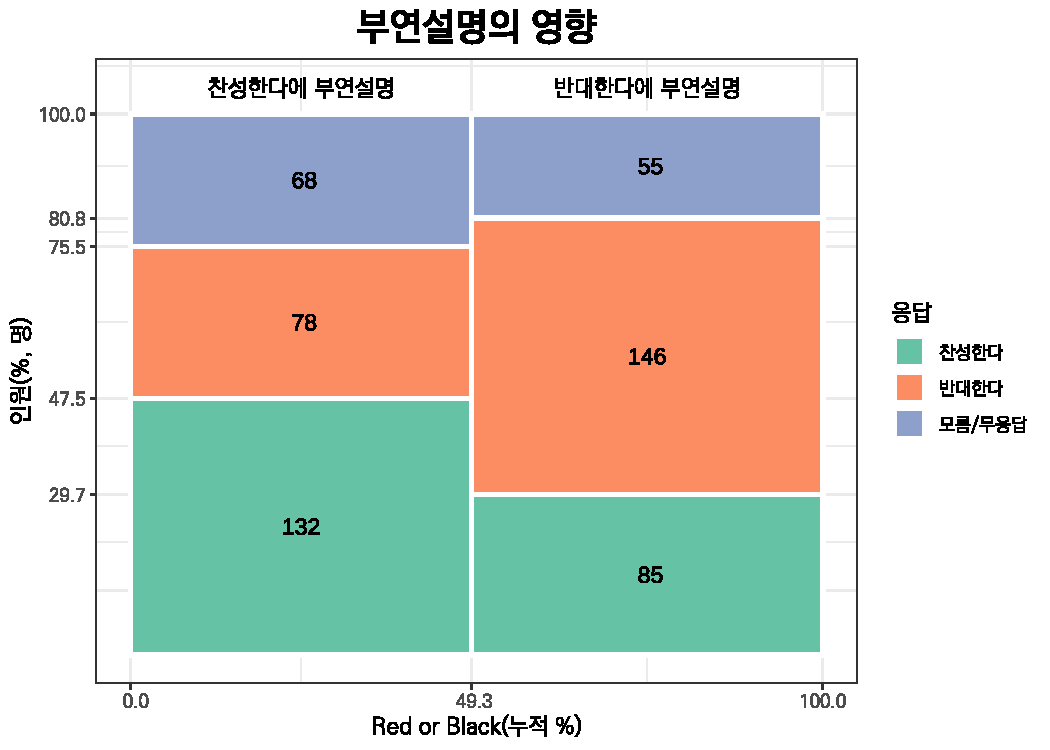
\includegraphics{_main_files/figure-latex/unnamed-chunk-95-1.pdf}

Mosaic Plot 은 이 집계결과를 시각적으로 잘 보여줍니다.

찬성을 유도하는 부연설명을 붙인 Red 에서 ``찬성한다''고 응답한 백분율이 높고, 반대를 유도하는 부연설명을 붙인 Black 에서 ``반대한다''고 응답한 백분율이 월등히 높은 것을 시각적으로 알 수 있습니다.

\section{마감 시간으로부터 제출 시간의 분포}\label{uxb9c8uxac10-uxc2dcuxac04uxc73cuxb85cuxbd80uxd130-uxc81cuxcd9c-uxc2dcuxac04uxc758-uxbd84uxd3ec-3}

\subsection{분포표}\label{uxbd84uxd3ecuxd45c-4}

\begin{longtable}[]{@{}
  >{\raggedright\arraybackslash}p{(\columnwidth - 30\tabcolsep) * \real{0.0863}}
  >{\raggedleft\arraybackslash}p{(\columnwidth - 30\tabcolsep) * \real{0.0576}}
  >{\raggedleft\arraybackslash}p{(\columnwidth - 30\tabcolsep) * \real{0.0576}}
  >{\raggedleft\arraybackslash}p{(\columnwidth - 30\tabcolsep) * \real{0.0576}}
  >{\raggedleft\arraybackslash}p{(\columnwidth - 30\tabcolsep) * \real{0.0576}}
  >{\raggedleft\arraybackslash}p{(\columnwidth - 30\tabcolsep) * \real{0.0576}}
  >{\raggedleft\arraybackslash}p{(\columnwidth - 30\tabcolsep) * \real{0.0576}}
  >{\raggedleft\arraybackslash}p{(\columnwidth - 30\tabcolsep) * \real{0.0576}}
  >{\raggedleft\arraybackslash}p{(\columnwidth - 30\tabcolsep) * \real{0.0576}}
  >{\raggedleft\arraybackslash}p{(\columnwidth - 30\tabcolsep) * \real{0.0576}}
  >{\raggedleft\arraybackslash}p{(\columnwidth - 30\tabcolsep) * \real{0.0647}}
  >{\raggedleft\arraybackslash}p{(\columnwidth - 30\tabcolsep) * \real{0.0719}}
  >{\raggedleft\arraybackslash}p{(\columnwidth - 30\tabcolsep) * \real{0.0719}}
  >{\raggedleft\arraybackslash}p{(\columnwidth - 30\tabcolsep) * \real{0.0719}}
  >{\raggedleft\arraybackslash}p{(\columnwidth - 30\tabcolsep) * \real{0.0719}}
  >{\centering\arraybackslash}p{(\columnwidth - 30\tabcolsep) * \real{0.0432}}@{}}
\caption{일 단위}\tabularnewline
\toprule\noalign{}
\begin{minipage}[b]{\linewidth}\raggedright
~
\end{minipage} & \begin{minipage}[b]{\linewidth}\raggedleft
{[}0,1{]}
\end{minipage} & \begin{minipage}[b]{\linewidth}\raggedleft
(1,2{]}
\end{minipage} & \begin{minipage}[b]{\linewidth}\raggedleft
(2,3{]}
\end{minipage} & \begin{minipage}[b]{\linewidth}\raggedleft
(3,4{]}
\end{minipage} & \begin{minipage}[b]{\linewidth}\raggedleft
(4,5{]}
\end{minipage} & \begin{minipage}[b]{\linewidth}\raggedleft
(5,6{]}
\end{minipage} & \begin{minipage}[b]{\linewidth}\raggedleft
(6,7{]}
\end{minipage} & \begin{minipage}[b]{\linewidth}\raggedleft
(7,8{]}
\end{minipage} & \begin{minipage}[b]{\linewidth}\raggedleft
(8,9{]}
\end{minipage} & \begin{minipage}[b]{\linewidth}\raggedleft
(9,10{]}
\end{minipage} & \begin{minipage}[b]{\linewidth}\raggedleft
(10,11{]}
\end{minipage} & \begin{minipage}[b]{\linewidth}\raggedleft
(11,12{]}
\end{minipage} & \begin{minipage}[b]{\linewidth}\raggedleft
(12,13{]}
\end{minipage} & \begin{minipage}[b]{\linewidth}\raggedleft
(13,14{]}
\end{minipage} & \begin{minipage}[b]{\linewidth}\centering
계
\end{minipage} \\
\midrule\noalign{}
\endfirsthead
\toprule\noalign{}
\begin{minipage}[b]{\linewidth}\raggedright
~
\end{minipage} & \begin{minipage}[b]{\linewidth}\raggedleft
{[}0,1{]}
\end{minipage} & \begin{minipage}[b]{\linewidth}\raggedleft
(1,2{]}
\end{minipage} & \begin{minipage}[b]{\linewidth}\raggedleft
(2,3{]}
\end{minipage} & \begin{minipage}[b]{\linewidth}\raggedleft
(3,4{]}
\end{minipage} & \begin{minipage}[b]{\linewidth}\raggedleft
(4,5{]}
\end{minipage} & \begin{minipage}[b]{\linewidth}\raggedleft
(5,6{]}
\end{minipage} & \begin{minipage}[b]{\linewidth}\raggedleft
(6,7{]}
\end{minipage} & \begin{minipage}[b]{\linewidth}\raggedleft
(7,8{]}
\end{minipage} & \begin{minipage}[b]{\linewidth}\raggedleft
(8,9{]}
\end{minipage} & \begin{minipage}[b]{\linewidth}\raggedleft
(9,10{]}
\end{minipage} & \begin{minipage}[b]{\linewidth}\raggedleft
(10,11{]}
\end{minipage} & \begin{minipage}[b]{\linewidth}\raggedleft
(11,12{]}
\end{minipage} & \begin{minipage}[b]{\linewidth}\raggedleft
(12,13{]}
\end{minipage} & \begin{minipage}[b]{\linewidth}\raggedleft
(13,14{]}
\end{minipage} & \begin{minipage}[b]{\linewidth}\centering
계
\end{minipage} \\
\midrule\noalign{}
\endhead
\bottomrule\noalign{}
\endlastfoot
\textbf{Red} & 71 & 15 & 13 & 4 & 10 & 3 & 6 & 46 & 20 & 22 & 14 & 20 & 16 & 18 & 278 \\
\textbf{Black} & 71 & 14 & 7 & 7 & 11 & 4 & 6 & 50 & 20 & 14 & 12 & 24 & 17 & 29 & 286 \\
\textbf{계} & 142 & 29 & 20 & 11 & 21 & 7 & 12 & 96 & 40 & 36 & 26 & 44 & 33 & 47 & 564 \\
\end{longtable}

분포표로부터 두 가지 문제를 살펴보겠습니다.

첫째, 날마다 고르게 제출하는가?

둘째, Red, Black 간에 통게적으로 유의한 차이가 있는가?

각 문제를 살펴보기 위해서는 분포표의 일부분을 대상으로 카이제곱 테스트를 수행합니다.

\subsection{날마다 고르게 제출하는가?}\label{uxb0a0uxb9c8uxb2e4-uxace0uxb974uxac8c-uxc81cuxcd9cuxd558uxb294uxac00-3}

\begin{longtable}[]{@{}
  >{\raggedleft\arraybackslash}p{(\columnwidth - 26\tabcolsep) * \real{0.0661}}
  >{\raggedleft\arraybackslash}p{(\columnwidth - 26\tabcolsep) * \real{0.0661}}
  >{\raggedleft\arraybackslash}p{(\columnwidth - 26\tabcolsep) * \real{0.0661}}
  >{\raggedleft\arraybackslash}p{(\columnwidth - 26\tabcolsep) * \real{0.0661}}
  >{\raggedleft\arraybackslash}p{(\columnwidth - 26\tabcolsep) * \real{0.0661}}
  >{\raggedleft\arraybackslash}p{(\columnwidth - 26\tabcolsep) * \real{0.0661}}
  >{\raggedleft\arraybackslash}p{(\columnwidth - 26\tabcolsep) * \real{0.0661}}
  >{\raggedleft\arraybackslash}p{(\columnwidth - 26\tabcolsep) * \real{0.0661}}
  >{\raggedleft\arraybackslash}p{(\columnwidth - 26\tabcolsep) * \real{0.0661}}
  >{\raggedleft\arraybackslash}p{(\columnwidth - 26\tabcolsep) * \real{0.0744}}
  >{\raggedleft\arraybackslash}p{(\columnwidth - 26\tabcolsep) * \real{0.0826}}
  >{\raggedleft\arraybackslash}p{(\columnwidth - 26\tabcolsep) * \real{0.0826}}
  >{\raggedleft\arraybackslash}p{(\columnwidth - 26\tabcolsep) * \real{0.0826}}
  >{\raggedleft\arraybackslash}p{(\columnwidth - 26\tabcolsep) * \real{0.0826}}@{}}
\toprule\noalign{}
\begin{minipage}[b]{\linewidth}\raggedleft
{[}0,1{]}
\end{minipage} & \begin{minipage}[b]{\linewidth}\raggedleft
(1,2{]}
\end{minipage} & \begin{minipage}[b]{\linewidth}\raggedleft
(2,3{]}
\end{minipage} & \begin{minipage}[b]{\linewidth}\raggedleft
(3,4{]}
\end{minipage} & \begin{minipage}[b]{\linewidth}\raggedleft
(4,5{]}
\end{minipage} & \begin{minipage}[b]{\linewidth}\raggedleft
(5,6{]}
\end{minipage} & \begin{minipage}[b]{\linewidth}\raggedleft
(6,7{]}
\end{minipage} & \begin{minipage}[b]{\linewidth}\raggedleft
(7,8{]}
\end{minipage} & \begin{minipage}[b]{\linewidth}\raggedleft
(8,9{]}
\end{minipage} & \begin{minipage}[b]{\linewidth}\raggedleft
(9,10{]}
\end{minipage} & \begin{minipage}[b]{\linewidth}\raggedleft
(10,11{]}
\end{minipage} & \begin{minipage}[b]{\linewidth}\raggedleft
(11,12{]}
\end{minipage} & \begin{minipage}[b]{\linewidth}\raggedleft
(12,13{]}
\end{minipage} & \begin{minipage}[b]{\linewidth}\raggedleft
(13,14{]}
\end{minipage} \\
\midrule\noalign{}
\endhead
\bottomrule\noalign{}
\endlastfoot
142 & 29 & 20 & 11 & 21 & 7 & 12 & 96 & 40 & 36 & 26 & 44 & 33 & 47 \\
\end{longtable}

\begin{longtable}[]{@{}
  >{\raggedleft\arraybackslash}p{(\columnwidth - 4\tabcolsep) * \real{0.2361}}
  >{\raggedleft\arraybackslash}p{(\columnwidth - 4\tabcolsep) * \real{0.0694}}
  >{\raggedleft\arraybackslash}p{(\columnwidth - 4\tabcolsep) * \real{0.2500}}@{}}
\caption{Chi-squared test for given probabilities: \texttt{.}}\tabularnewline
\toprule\noalign{}
\begin{minipage}[b]{\linewidth}\raggedleft
Test statistic
\end{minipage} & \begin{minipage}[b]{\linewidth}\raggedleft
df
\end{minipage} & \begin{minipage}[b]{\linewidth}\raggedleft
P value
\end{minipage} \\
\midrule\noalign{}
\endfirsthead
\toprule\noalign{}
\begin{minipage}[b]{\linewidth}\raggedleft
Test statistic
\end{minipage} & \begin{minipage}[b]{\linewidth}\raggedleft
df
\end{minipage} & \begin{minipage}[b]{\linewidth}\raggedleft
P value
\end{minipage} \\
\midrule\noalign{}
\endhead
\bottomrule\noalign{}
\endlastfoot
433.4 & 13 & 1.915e-84 * * * \\
\end{longtable}

날마다 고르게 제출하는지 알아 보았습니다.

분포표의 ``계''행에서 '계'열을 제외하고 카이제곱테스트를 수행합니다.

분포표 만으로도 쉽게 파악할 수 있지만 카이제곱테스트가 명확히 해 줍니다.

카이제곱 통계량은 433.43, 자유도는 13.00, p-value 는 1.9e-84 이므로 결코 고르게 제출한다고 말할 수 없습니다.

막대그래프로 살펴 보겠습니다.

\subsection{막대그래프}\label{uxb9c9uxb300uxadf8uxb798uxd504-4}

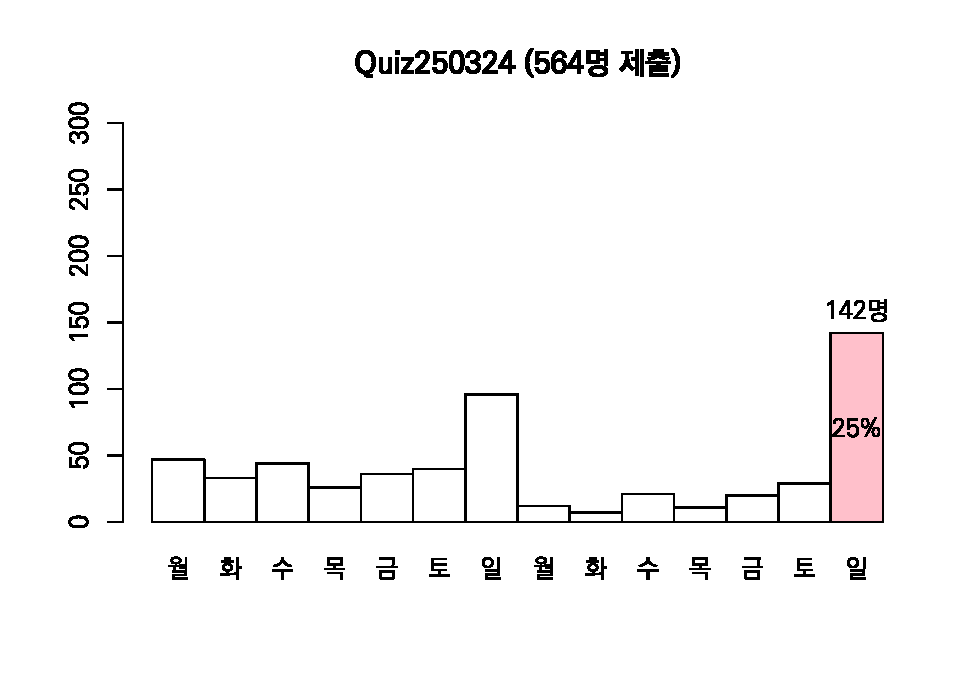
\includegraphics{_main_files/figure-latex/unnamed-chunk-98-1.pdf}

막대그래프는 총 제출인원 564(명) 중에 142(명), 25(\%)가 마감일에 몰리는 것을 명확히 보여주고 있습니다.

\subsection{Red, Black 간에 닮았는가?}\label{red-black-uxac04uxc5d0-uxb2eeuxc558uxb294uxac00-3}

\begin{longtable}[]{@{}
  >{\raggedright\arraybackslash}p{(\columnwidth - 28\tabcolsep) * \real{0.0902}}
  >{\raggedleft\arraybackslash}p{(\columnwidth - 28\tabcolsep) * \real{0.0602}}
  >{\raggedleft\arraybackslash}p{(\columnwidth - 28\tabcolsep) * \real{0.0602}}
  >{\raggedleft\arraybackslash}p{(\columnwidth - 28\tabcolsep) * \real{0.0602}}
  >{\raggedleft\arraybackslash}p{(\columnwidth - 28\tabcolsep) * \real{0.0602}}
  >{\raggedleft\arraybackslash}p{(\columnwidth - 28\tabcolsep) * \real{0.0602}}
  >{\raggedleft\arraybackslash}p{(\columnwidth - 28\tabcolsep) * \real{0.0602}}
  >{\raggedleft\arraybackslash}p{(\columnwidth - 28\tabcolsep) * \real{0.0602}}
  >{\raggedleft\arraybackslash}p{(\columnwidth - 28\tabcolsep) * \real{0.0602}}
  >{\raggedleft\arraybackslash}p{(\columnwidth - 28\tabcolsep) * \real{0.0602}}
  >{\raggedleft\arraybackslash}p{(\columnwidth - 28\tabcolsep) * \real{0.0677}}
  >{\raggedleft\arraybackslash}p{(\columnwidth - 28\tabcolsep) * \real{0.0752}}
  >{\raggedleft\arraybackslash}p{(\columnwidth - 28\tabcolsep) * \real{0.0752}}
  >{\raggedleft\arraybackslash}p{(\columnwidth - 28\tabcolsep) * \real{0.0752}}
  >{\raggedleft\arraybackslash}p{(\columnwidth - 28\tabcolsep) * \real{0.0752}}@{}}
\toprule\noalign{}
\begin{minipage}[b]{\linewidth}\raggedright
~
\end{minipage} & \begin{minipage}[b]{\linewidth}\raggedleft
{[}0,1{]}
\end{minipage} & \begin{minipage}[b]{\linewidth}\raggedleft
(1,2{]}
\end{minipage} & \begin{minipage}[b]{\linewidth}\raggedleft
(2,3{]}
\end{minipage} & \begin{minipage}[b]{\linewidth}\raggedleft
(3,4{]}
\end{minipage} & \begin{minipage}[b]{\linewidth}\raggedleft
(4,5{]}
\end{minipage} & \begin{minipage}[b]{\linewidth}\raggedleft
(5,6{]}
\end{minipage} & \begin{minipage}[b]{\linewidth}\raggedleft
(6,7{]}
\end{minipage} & \begin{minipage}[b]{\linewidth}\raggedleft
(7,8{]}
\end{minipage} & \begin{minipage}[b]{\linewidth}\raggedleft
(8,9{]}
\end{minipage} & \begin{minipage}[b]{\linewidth}\raggedleft
(9,10{]}
\end{minipage} & \begin{minipage}[b]{\linewidth}\raggedleft
(10,11{]}
\end{minipage} & \begin{minipage}[b]{\linewidth}\raggedleft
(11,12{]}
\end{minipage} & \begin{minipage}[b]{\linewidth}\raggedleft
(12,13{]}
\end{minipage} & \begin{minipage}[b]{\linewidth}\raggedleft
(13,14{]}
\end{minipage} \\
\midrule\noalign{}
\endhead
\bottomrule\noalign{}
\endlastfoot
\textbf{Red} & 71 & 15 & 13 & 4 & 10 & 3 & 6 & 46 & 20 & 22 & 14 & 20 & 16 & 18 \\
\textbf{Black} & 71 & 14 & 7 & 7 & 11 & 4 & 6 & 50 & 20 & 14 & 12 & 24 & 17 & 29 \\
\end{longtable}

\begin{longtable}[]{@{}
  >{\raggedleft\arraybackslash}p{(\columnwidth - 4\tabcolsep) * \real{0.2361}}
  >{\raggedleft\arraybackslash}p{(\columnwidth - 4\tabcolsep) * \real{0.0694}}
  >{\raggedleft\arraybackslash}p{(\columnwidth - 4\tabcolsep) * \real{0.1389}}@{}}
\caption{Pearson's Chi-squared test: \texttt{.}}\tabularnewline
\toprule\noalign{}
\begin{minipage}[b]{\linewidth}\raggedleft
Test statistic
\end{minipage} & \begin{minipage}[b]{\linewidth}\raggedleft
df
\end{minipage} & \begin{minipage}[b]{\linewidth}\raggedleft
P value
\end{minipage} \\
\midrule\noalign{}
\endfirsthead
\toprule\noalign{}
\begin{minipage}[b]{\linewidth}\raggedleft
Test statistic
\end{minipage} & \begin{minipage}[b]{\linewidth}\raggedleft
df
\end{minipage} & \begin{minipage}[b]{\linewidth}\raggedleft
P value
\end{minipage} \\
\midrule\noalign{}
\endhead
\bottomrule\noalign{}
\endlastfoot
7.798 & 13 & 0.8565 \\
\end{longtable}

제출시간의 분포가 Red, Black 간에 닮았는지 알아 보았습니다.

이번에는 분포표의 첫번째와 두번째 행, '계'열을 제외한 나머지 열에 대해서 카이제곱테스트를 수행합니다.

카이제곱 통계량은 7.798, 자유도는 13, p-value 는 0.8565 이므로 제출 시간의 분포는 Red, Black 간에 통계적으로 유의한 차이가 관찰되지 않습니다.

이 사실을 Mosaic Plot 을 이용하여 시각적으로 살펴보겠습니다.

닮았다고 느껴지나요?

\subsection{Mosaic Plot}\label{mosaic-plot-7}

\includegraphics{_main_files/figure-latex/unnamed-chunk-100-1.pdf}

\chapter{5주차 데이터 실험 집계}\label{uxc8fcuxcc28-uxb370uxc774uxd130-uxc2e4uxd5d8-uxc9d1uxacc4-4}

\section{실험의 목적}\label{uxc2e4uxd5d8uxc758-uxbaa9uxc801-4}

5주차 구글 예습 설문지 집계결과를 분석합니다.

Q1\textasciitilde Q6에서는 랜덤화의 효과로 Red, Black 이 얼마나 닮았는지 알아봅니다.

Q7에서는 컵에 우유를 반을 쏟은 상황에서 긍정적인 단어를 읽은 그룹하고 부정적인 단어를 읽은 그룹 사이에 어떠한 인식의 차이가 발생하는 지 살펴봅니다.

끝으로 제출시간의 분포가 날마다 고른지, Red, Black 간에는 닮았는지 알아봅니다.

\subsection{Red, Black을 잘못 표시한 사람들}\label{red-blackuxc744-uxc798uxbabb-uxd45cuxc2dcuxd55c-uxc0acuxb78cuxb4e4-4}

\begin{longtable}[]{@{}
  >{\raggedright\arraybackslash}p{(\columnwidth - 4\tabcolsep) * \real{0.3611}}
  >{\centering\arraybackslash}p{(\columnwidth - 4\tabcolsep) * \real{0.2778}}
  >{\centering\arraybackslash}p{(\columnwidth - 4\tabcolsep) * \real{0.3056}}@{}}
\toprule\noalign{}
\begin{minipage}[b]{\linewidth}\raggedright
~
\end{minipage} & \begin{minipage}[b]{\linewidth}\centering
Red(구글예습퀴즈)
\end{minipage} & \begin{minipage}[b]{\linewidth}\centering
Black(구글예습퀴즈)
\end{minipage} \\
\midrule\noalign{}
\endhead
\bottomrule\noalign{}
\endlastfoot
\textbf{Red(랜덤화출석부)} & 274 & 1 \\
\textbf{Black(랜덤화출석부)} & 3 & 280 \\
\textbf{계} & 277 & 281 \\
\end{longtable}

랜덤화출석부에 있는 Red, Black 과 실제 구글설문에 올린 Red, Black 이 다른 사람들의 수효는 4명입니다.

Red를 Black 이라고 한 사람이 1명, Black 을 Red 라고 한 사람이 3명입니다.

두 가지 방법으로 분석합니다.

우선 Red, Black 을 잘못 선택한 4명을 랜덤하게 둘로 나누면 어느 한 쪽 집단에 들어갈 기대인원은 4명을 둘로 나눈 2(명)이고, 표준오차는 4의 제곱근에 1/2을 곱해 준 1명이 됩니다.

실제로 Red를 Black 이라고 한 사람수, 1명이나 Black 을 Red 라고 한 사람수, 3명은 기대인원으로부터 표준오차 범위는 벗어 나지만 표준오차 두 배 범위에는 잘 들어갑니다.

두 번째 분석 방법은 확률을 계산해 보는 것입니다.

Red, Black 을 잘못 선택한 4명을 랜덤하게 둘로 나눌 때, 실제로 관찰된 3명 이상이나 1명이하로 잘못 선택한 사람수가 나올 가능성은 얼마나 되는가 입니다.

이 경우 공평한 동전던지기를 확률 법칙으로 표현한 이항분포로부터 계산할 수 있습니다.

시행횟수가 4이고 한 번 시행에서 성공확률이 1/2 인 이항분포에서 성공횟수가 1이하이거나 3이상을 관찰할 확률은 0.625입니다.

공평한 동전 던지기에서 앞면이 1개 이하 나오는 확률은 3개 이상 나오는 확률과 같기 때문에 사실상 한쪽만 계산해서 2배 해 주면 됩니다.

이 값을 p-value 라고 하는데, p-value가 0.05보다 작을 때 \textbf{통계적으로 유의한 차이를 관찰}하였다고 말합니다.

즉, 공평한 동전을 던지는 것과 같은 과정이라고 가정하였을 때 실제로 관찰된 값들이 가정으로부터 얼마나 떨어져 있는지를 표현한 것입니다.

0.05는 이런 실험을 스무 번 정도 반복하면 1번 나올 정도로 드문 사건을 의미합니다.

즉 가정이 잘못되었다는 것입니다.

그런데 Red, Black 을 잘못 표시한 사람들의 분포에서 관찰된 p-value 는 0.05와는 비교도 안될 정도로 큰 값입니다.

따라서 두 집단이 랜덤화 효과가 작동하여 \textbf{통계적으로 유의한 차이를 보이지 않는다}고 할 수 있습니다.

\subsection{응답인원의 Red, Black}\label{uxc751uxb2f5uxc778uxc6d0uxc758-red-black-4}

Red 로 응답한 인원은 277명, Black 에 응답한 인원은 281명입니다.

전체 응답인원 558 명을 랜덤하게 둘로 나눌 때 어느 한 쪽의 기대인원은 전체 응답인원의 절반인 279명이고, 표준오차는 전체 응답인원의 제곱근에 1/2을 곱해 준 11.8 명입니다.

따라서 Red, Black 각 그룹에 관찰된 인원은 기대인원으로부터 표준오차 범위 안에 들어갑니다.

\section{Q1. 한글의 문자 유형}\label{q1.-uxd55cuxae00uxc758-uxbb38uxc790-uxc720uxd615}

\begin{flushleft}\includegraphics[width=0.75\linewidth]{./pics/Quiz210323_Q1} \end{flushleft}

\subsection{한글은 민주 문자}\label{uxd55cuxae00uxc740-uxbbfcuxc8fc-uxbb38uxc790}

\begin{longtable}[]{@{}
  >{\raggedright\arraybackslash}p{(\columnwidth - 6\tabcolsep) * \real{0.1667}}
  >{\centering\arraybackslash}p{(\columnwidth - 6\tabcolsep) * \real{0.1667}}
  >{\centering\arraybackslash}p{(\columnwidth - 6\tabcolsep) * \real{0.1944}}
  >{\centering\arraybackslash}p{(\columnwidth - 6\tabcolsep) * \real{0.0833}}@{}}
\toprule\noalign{}
\begin{minipage}[b]{\linewidth}\raggedright
~
\end{minipage} & \begin{minipage}[b]{\linewidth}\centering
민주 문자
\end{minipage} & \begin{minipage}[b]{\linewidth}\centering
엘리트 문자
\end{minipage} & \begin{minipage}[b]{\linewidth}\centering
계
\end{minipage} \\
\midrule\noalign{}
\endhead
\bottomrule\noalign{}
\endlastfoot
\textbf{Red} & 261 & 16 & 277 \\
\textbf{Black} & 263 & 18 & 281 \\
\textbf{계} & 524 & 34 & 558 \\
\end{longtable}

\begin{longtable}[]{@{}
  >{\raggedleft\arraybackslash}p{(\columnwidth - 4\tabcolsep) * \real{0.2361}}
  >{\raggedleft\arraybackslash}p{(\columnwidth - 4\tabcolsep) * \real{0.0694}}
  >{\raggedleft\arraybackslash}p{(\columnwidth - 4\tabcolsep) * \real{0.1389}}@{}}
\caption{Pearson's Chi-squared test with Yates' continuity correction: \texttt{.}}\tabularnewline
\toprule\noalign{}
\begin{minipage}[b]{\linewidth}\raggedleft
Test statistic
\end{minipage} & \begin{minipage}[b]{\linewidth}\raggedleft
df
\end{minipage} & \begin{minipage}[b]{\linewidth}\raggedleft
P value
\end{minipage} \\
\midrule\noalign{}
\endfirsthead
\toprule\noalign{}
\begin{minipage}[b]{\linewidth}\raggedleft
Test statistic
\end{minipage} & \begin{minipage}[b]{\linewidth}\raggedleft
df
\end{minipage} & \begin{minipage}[b]{\linewidth}\raggedleft
P value
\end{minipage} \\
\midrule\noalign{}
\endhead
\bottomrule\noalign{}
\endlastfoot
0.01791 & 1 & 0.8935 \\
\end{longtable}

Q1의 집계 결과가 Red, Black 간에 통계적으로 유의한 차이가 있는지 알아보기 위하여 카이제곱 테스트를 수행하였습니다.

그 결과 카이제곱 통계량은 0.018, 자유도는 1 , p-value 는 0.8935이므로 Red, Black 간에 통계적으로 유의한 차이를 보이지 않습니다.

실제로 닮은 게 느껴집니까?

\subsection{한글은 민주 문자(\%)}\label{uxd55cuxae00uxc740-uxbbfcuxc8fc-uxbb38uxc790-1}

\begin{longtable}[]{@{}
  >{\centering\arraybackslash}p{(\columnwidth - 4\tabcolsep) * \real{0.1667}}
  >{\centering\arraybackslash}p{(\columnwidth - 4\tabcolsep) * \real{0.1944}}
  >{\centering\arraybackslash}p{(\columnwidth - 4\tabcolsep) * \real{0.1111}}@{}}
\toprule\noalign{}
\begin{minipage}[b]{\linewidth}\centering
민주 문자
\end{minipage} & \begin{minipage}[b]{\linewidth}\centering
엘리트 문자
\end{minipage} & \begin{minipage}[b]{\linewidth}\centering
계
\end{minipage} \\
\midrule\noalign{}
\endhead
\bottomrule\noalign{}
\endlastfoot
93.9 & 6.1 & 100.0 \\
\end{longtable}

정답률은 Red, Black 을 합하여 계산하는데, 93.9(\%) 입니다.

\section{Q2. 정보혁명과 문자 체계}\label{q2.-uxc815uxbcf4uxd601uxba85uxacfc-uxbb38uxc790-uxccb4uxacc4}

\begin{flushleft}\includegraphics[width=0.75\linewidth]{./pics/Quiz210323_Q2} \end{flushleft}

\subsection{정보혁명을 이끄는 문자는 한글(집계표)}\label{uxc815uxbcf4uxd601uxba85uxc744-uxc774uxb044uxb294-uxbb38uxc790uxb294-uxd55cuxae00uxc9d1uxacc4uxd45c}

\begin{longtable}[]{@{}
  >{\raggedright\arraybackslash}p{(\columnwidth - 6\tabcolsep) * \real{0.1667}}
  >{\centering\arraybackslash}p{(\columnwidth - 6\tabcolsep) * \real{0.0972}}
  >{\centering\arraybackslash}p{(\columnwidth - 6\tabcolsep) * \real{0.0972}}
  >{\centering\arraybackslash}p{(\columnwidth - 6\tabcolsep) * \real{0.0972}}@{}}
\toprule\noalign{}
\begin{minipage}[b]{\linewidth}\raggedright
~
\end{minipage} & \begin{minipage}[b]{\linewidth}\centering
한자
\end{minipage} & \begin{minipage}[b]{\linewidth}\centering
한글
\end{minipage} & \begin{minipage}[b]{\linewidth}\centering
계
\end{minipage} \\
\midrule\noalign{}
\endhead
\bottomrule\noalign{}
\endlastfoot
\textbf{Red} & 23 & 254 & 277 \\
\textbf{Black} & 16 & 265 & 281 \\
\textbf{계} & 39 & 519 & 558 \\
\end{longtable}

\begin{longtable}[]{@{}
  >{\raggedleft\arraybackslash}p{(\columnwidth - 4\tabcolsep) * \real{0.2361}}
  >{\raggedleft\arraybackslash}p{(\columnwidth - 4\tabcolsep) * \real{0.0694}}
  >{\raggedleft\arraybackslash}p{(\columnwidth - 4\tabcolsep) * \real{0.1389}}@{}}
\caption{Pearson's Chi-squared test with Yates' continuity correction: \texttt{.}}\tabularnewline
\toprule\noalign{}
\begin{minipage}[b]{\linewidth}\raggedleft
Test statistic
\end{minipage} & \begin{minipage}[b]{\linewidth}\raggedleft
df
\end{minipage} & \begin{minipage}[b]{\linewidth}\raggedleft
P value
\end{minipage} \\
\midrule\noalign{}
\endfirsthead
\toprule\noalign{}
\begin{minipage}[b]{\linewidth}\raggedleft
Test statistic
\end{minipage} & \begin{minipage}[b]{\linewidth}\raggedleft
df
\end{minipage} & \begin{minipage}[b]{\linewidth}\raggedleft
P value
\end{minipage} \\
\midrule\noalign{}
\endhead
\bottomrule\noalign{}
\endlastfoot
1.087 & 1 & 0.2971 \\
\end{longtable}

Q2의 집계 결과가 Red, Black 간에 통계적으로 유의한 차이가 있는지 알아보기 위하여 카이제곱 테스트를 수행하였습니다.

그 결과 카이제곱 통계량은 1.09, 자유도는 1, p-value 는 0.30이므로 Red, Black 간에 통계적으로 유의한 차이를 보이지 않습니다.

실제로 닮은 게 느껴집니까?

\subsection{정보혁명을 이끄는 문자는 한글(\%)}\label{uxc815uxbcf4uxd601uxba85uxc744-uxc774uxb044uxb294-uxbb38uxc790uxb294-uxd55cuxae00}

\begin{longtable}[]{@{}
  >{\centering\arraybackslash}p{(\columnwidth - 4\tabcolsep) * \real{0.0972}}
  >{\centering\arraybackslash}p{(\columnwidth - 4\tabcolsep) * \real{0.0972}}
  >{\centering\arraybackslash}p{(\columnwidth - 4\tabcolsep) * \real{0.1111}}@{}}
\toprule\noalign{}
\begin{minipage}[b]{\linewidth}\centering
한자
\end{minipage} & \begin{minipage}[b]{\linewidth}\centering
한글
\end{minipage} & \begin{minipage}[b]{\linewidth}\centering
계
\end{minipage} \\
\midrule\noalign{}
\endhead
\bottomrule\noalign{}
\endlastfoot
7.0 & 93.0 & 100.0 \\
\end{longtable}

정답률은 Red, Black 을 합하여 계산하는데, 93.0(\%) 입니다.

\section{Q3. 알기 힘든 전문 용어}\label{q3.-uxc54cuxae30-uxd798uxb4e0-uxc804uxbb38-uxc6a9uxc5b4}

\begin{flushleft}\includegraphics[width=0.75\linewidth]{./pics/Quiz210323_Q3} \end{flushleft}

\subsection{몇 개나 아나요?(집계표)}\label{uxba87-uxac1cuxb098-uxc544uxb098uxc694uxc9d1uxacc4uxd45c}

\begin{longtable}[]{@{}
  >{\raggedright\arraybackslash}p{(\columnwidth - 12\tabcolsep) * \real{0.1667}}
  >{\centering\arraybackslash}p{(\columnwidth - 12\tabcolsep) * \real{0.1944}}
  >{\centering\arraybackslash}p{(\columnwidth - 12\tabcolsep) * \real{0.0833}}
  >{\centering\arraybackslash}p{(\columnwidth - 12\tabcolsep) * \real{0.0833}}
  >{\centering\arraybackslash}p{(\columnwidth - 12\tabcolsep) * \real{0.0833}}
  >{\centering\arraybackslash}p{(\columnwidth - 12\tabcolsep) * \real{0.0833}}
  >{\centering\arraybackslash}p{(\columnwidth - 12\tabcolsep) * \real{0.0833}}@{}}
\toprule\noalign{}
\begin{minipage}[b]{\linewidth}\raggedright
~
\end{minipage} & \begin{minipage}[b]{\linewidth}\centering
하나도 없다
\end{minipage} & \begin{minipage}[b]{\linewidth}\centering
1개
\end{minipage} & \begin{minipage}[b]{\linewidth}\centering
2개
\end{minipage} & \begin{minipage}[b]{\linewidth}\centering
3개
\end{minipage} & \begin{minipage}[b]{\linewidth}\centering
4개
\end{minipage} & \begin{minipage}[b]{\linewidth}\centering
계
\end{minipage} \\
\midrule\noalign{}
\endhead
\bottomrule\noalign{}
\endlastfoot
\textbf{Red} & 138 & 72 & 41 & 15 & 11 & 277 \\
\textbf{Black} & 150 & 70 & 40 & 11 & 10 & 281 \\
\textbf{계} & 288 & 142 & 81 & 26 & 21 & 558 \\
\end{longtable}

\begin{longtable}[]{@{}
  >{\raggedleft\arraybackslash}p{(\columnwidth - 4\tabcolsep) * \real{0.2361}}
  >{\raggedleft\arraybackslash}p{(\columnwidth - 4\tabcolsep) * \real{0.0694}}
  >{\raggedleft\arraybackslash}p{(\columnwidth - 4\tabcolsep) * \real{0.1389}}@{}}
\caption{Pearson's Chi-squared test: \texttt{.}}\tabularnewline
\toprule\noalign{}
\begin{minipage}[b]{\linewidth}\raggedleft
Test statistic
\end{minipage} & \begin{minipage}[b]{\linewidth}\raggedleft
df
\end{minipage} & \begin{minipage}[b]{\linewidth}\raggedleft
P value
\end{minipage} \\
\midrule\noalign{}
\endfirsthead
\toprule\noalign{}
\begin{minipage}[b]{\linewidth}\raggedleft
Test statistic
\end{minipage} & \begin{minipage}[b]{\linewidth}\raggedleft
df
\end{minipage} & \begin{minipage}[b]{\linewidth}\raggedleft
P value
\end{minipage} \\
\midrule\noalign{}
\endhead
\bottomrule\noalign{}
\endlastfoot
1.175 & 4 & 0.8822 \\
\end{longtable}

Q3의 집계 결과가 Red, Black 간에 통계적으로 유의한 차이가 있는지 알아보기 위하여 카이제곱 테스트를 수행하였습니다.

그 결과 카이제곱 통계량은 1.175, 자유도는 4, p-value 는 0.8822이므로 Red, Black 간에 통계적으로 유의한 차이를 보이지 않습니다.

실제로 닮은 게 느껴집니까?

\subsection{몇 개나 아나요?(\%)}\label{uxba87-uxac1cuxb098-uxc544uxb098uxc694}

\begin{longtable}[]{@{}
  >{\centering\arraybackslash}p{(\columnwidth - 10\tabcolsep) * \real{0.1944}}
  >{\centering\arraybackslash}p{(\columnwidth - 10\tabcolsep) * \real{0.0972}}
  >{\centering\arraybackslash}p{(\columnwidth - 10\tabcolsep) * \real{0.0972}}
  >{\centering\arraybackslash}p{(\columnwidth - 10\tabcolsep) * \real{0.0833}}
  >{\centering\arraybackslash}p{(\columnwidth - 10\tabcolsep) * \real{0.0833}}
  >{\centering\arraybackslash}p{(\columnwidth - 10\tabcolsep) * \real{0.1111}}@{}}
\toprule\noalign{}
\begin{minipage}[b]{\linewidth}\centering
하나도 없다
\end{minipage} & \begin{minipage}[b]{\linewidth}\centering
1개
\end{minipage} & \begin{minipage}[b]{\linewidth}\centering
2개
\end{minipage} & \begin{minipage}[b]{\linewidth}\centering
3개
\end{minipage} & \begin{minipage}[b]{\linewidth}\centering
4개
\end{minipage} & \begin{minipage}[b]{\linewidth}\centering
계
\end{minipage} \\
\midrule\noalign{}
\endhead
\bottomrule\noalign{}
\endlastfoot
51.6 & 25.4 & 14.5 & 4.7 & 3.8 & 100.0 \\
\end{longtable}

물론, 이 문제에는 정답이 없으므로 정답률은 의미가 없습니다.

가장 많은 비율로 응답한 것이 ``하나도 없다''이고 51.6(\%) 입니다.

\section{Q4. 해방직후 비문해율}\label{q4.-uxd574uxbc29uxc9c1uxd6c4-uxbe44uxbb38uxd574uxc728}

\begin{flushleft}\includegraphics[width=0.75\linewidth]{./pics/Quiz210323_Q4} \end{flushleft}

\subsection{집계}\label{uxc9d1uxacc4-2}

\begin{longtable}[]{@{}
  >{\raggedright\arraybackslash}p{(\columnwidth - 12\tabcolsep) * \real{0.1667}}
  >{\raggedleft\arraybackslash}p{(\columnwidth - 12\tabcolsep) * \real{0.0833}}
  >{\raggedleft\arraybackslash}p{(\columnwidth - 12\tabcolsep) * \real{0.0833}}
  >{\raggedleft\arraybackslash}p{(\columnwidth - 12\tabcolsep) * \real{0.0833}}
  >{\raggedleft\arraybackslash}p{(\columnwidth - 12\tabcolsep) * \real{0.0833}}
  >{\raggedleft\arraybackslash}p{(\columnwidth - 12\tabcolsep) * \real{0.0833}}
  >{\centering\arraybackslash}p{(\columnwidth - 12\tabcolsep) * \real{0.0833}}@{}}
\toprule\noalign{}
\begin{minipage}[b]{\linewidth}\raggedright
~
\end{minipage} & \begin{minipage}[b]{\linewidth}\raggedleft
90\%
\end{minipage} & \begin{minipage}[b]{\linewidth}\raggedleft
80\%
\end{minipage} & \begin{minipage}[b]{\linewidth}\raggedleft
50\%
\end{minipage} & \begin{minipage}[b]{\linewidth}\raggedleft
20\%
\end{minipage} & \begin{minipage}[b]{\linewidth}\raggedleft
10\%
\end{minipage} & \begin{minipage}[b]{\linewidth}\centering
계
\end{minipage} \\
\midrule\noalign{}
\endhead
\bottomrule\noalign{}
\endlastfoot
\textbf{Red} & 13 & 198 & 27 & 28 & 11 & 277 \\
\textbf{Black} & 15 & 193 & 35 & 23 & 15 & 281 \\
\textbf{계} & 28 & 391 & 62 & 51 & 26 & 558 \\
\end{longtable}

\begin{longtable}[]{@{}
  >{\raggedleft\arraybackslash}p{(\columnwidth - 4\tabcolsep) * \real{0.2361}}
  >{\raggedleft\arraybackslash}p{(\columnwidth - 4\tabcolsep) * \real{0.0694}}
  >{\raggedleft\arraybackslash}p{(\columnwidth - 4\tabcolsep) * \real{0.1389}}@{}}
\caption{Pearson's Chi-squared test: \texttt{.}}\tabularnewline
\toprule\noalign{}
\begin{minipage}[b]{\linewidth}\raggedleft
Test statistic
\end{minipage} & \begin{minipage}[b]{\linewidth}\raggedleft
df
\end{minipage} & \begin{minipage}[b]{\linewidth}\raggedleft
P value
\end{minipage} \\
\midrule\noalign{}
\endfirsthead
\toprule\noalign{}
\begin{minipage}[b]{\linewidth}\raggedleft
Test statistic
\end{minipage} & \begin{minipage}[b]{\linewidth}\raggedleft
df
\end{minipage} & \begin{minipage}[b]{\linewidth}\raggedleft
P value
\end{minipage} \\
\midrule\noalign{}
\endhead
\bottomrule\noalign{}
\endlastfoot
2.316 & 4 & 0.6778 \\
\end{longtable}

Q4의 집계 결과가 Red, Black 간에 통계적으로 유의한 차이가 있는지 알아보기 위하여 카이제곱 테스트를 수행하였습니다.

그 결과 카이제곱 통계량은 2.316, 자유도는 4, p-value 는 0.6778이므로 Red, Black 간에 통계적으로 유의한 차이를 보이지 않습니다.

실제로 닮은 게 느껴집니까?

\subsection{\%}\label{section}

\begin{longtable}[]{@{}
  >{\raggedleft\arraybackslash}p{(\columnwidth - 10\tabcolsep) * \real{0.0833}}
  >{\raggedleft\arraybackslash}p{(\columnwidth - 10\tabcolsep) * \real{0.0972}}
  >{\raggedleft\arraybackslash}p{(\columnwidth - 10\tabcolsep) * \real{0.0972}}
  >{\raggedleft\arraybackslash}p{(\columnwidth - 10\tabcolsep) * \real{0.0833}}
  >{\raggedleft\arraybackslash}p{(\columnwidth - 10\tabcolsep) * \real{0.0833}}
  >{\centering\arraybackslash}p{(\columnwidth - 10\tabcolsep) * \real{0.1111}}@{}}
\toprule\noalign{}
\begin{minipage}[b]{\linewidth}\raggedleft
90\%
\end{minipage} & \begin{minipage}[b]{\linewidth}\raggedleft
80\%
\end{minipage} & \begin{minipage}[b]{\linewidth}\raggedleft
50\%
\end{minipage} & \begin{minipage}[b]{\linewidth}\raggedleft
20\%
\end{minipage} & \begin{minipage}[b]{\linewidth}\raggedleft
10\%
\end{minipage} & \begin{minipage}[b]{\linewidth}\centering
계
\end{minipage} \\
\midrule\noalign{}
\endhead
\bottomrule\noalign{}
\endlastfoot
5.0 & 70.1 & 11.1 & 9.1 & 4.7 & 100.0 \\
\end{longtable}

정답률은 Red, Black 을 합하여 계산하는데, 70.1(\%) 입니다.

\section{Q5. 세대간 문해력 격차}\label{q5.-uxc138uxb300uxac04-uxbb38uxd574uxb825-uxaca9uxcc28}

\begin{flushleft}\includegraphics[width=0.75\linewidth]{./pics/Quiz210323_Q5} \end{flushleft}

\subsection{집계}\label{uxc9d1uxacc4-3}

\begin{longtable}[]{@{}
  >{\raggedright\arraybackslash}p{(\columnwidth - 10\tabcolsep) * \real{0.1667}}
  >{\centering\arraybackslash}p{(\columnwidth - 10\tabcolsep) * \real{0.1528}}
  >{\centering\arraybackslash}p{(\columnwidth - 10\tabcolsep) * \real{0.0972}}
  >{\centering\arraybackslash}p{(\columnwidth - 10\tabcolsep) * \real{0.1528}}
  >{\centering\arraybackslash}p{(\columnwidth - 10\tabcolsep) * \real{0.0972}}
  >{\centering\arraybackslash}p{(\columnwidth - 10\tabcolsep) * \real{0.0972}}@{}}
\toprule\noalign{}
\begin{minipage}[b]{\linewidth}\raggedright
~
\end{minipage} & \begin{minipage}[b]{\linewidth}\centering
대한민국
\end{minipage} & \begin{minipage}[b]{\linewidth}\centering
영국
\end{minipage} & \begin{minipage}[b]{\linewidth}\centering
이탈리아
\end{minipage} & \begin{minipage}[b]{\linewidth}\centering
미국
\end{minipage} & \begin{minipage}[b]{\linewidth}\centering
계
\end{minipage} \\
\midrule\noalign{}
\endhead
\bottomrule\noalign{}
\endlastfoot
\textbf{Red} & 212 & 18 & 18 & 29 & 277 \\
\textbf{Black} & 219 & 14 & 15 & 33 & 281 \\
\textbf{계} & 431 & 32 & 33 & 62 & 558 \\
\end{longtable}

\begin{longtable}[]{@{}
  >{\raggedleft\arraybackslash}p{(\columnwidth - 4\tabcolsep) * \real{0.2361}}
  >{\raggedleft\arraybackslash}p{(\columnwidth - 4\tabcolsep) * \real{0.0694}}
  >{\raggedleft\arraybackslash}p{(\columnwidth - 4\tabcolsep) * \real{0.1389}}@{}}
\caption{Pearson's Chi-squared test: \texttt{.}}\tabularnewline
\toprule\noalign{}
\begin{minipage}[b]{\linewidth}\raggedleft
Test statistic
\end{minipage} & \begin{minipage}[b]{\linewidth}\raggedleft
df
\end{minipage} & \begin{minipage}[b]{\linewidth}\raggedleft
P value
\end{minipage} \\
\midrule\noalign{}
\endfirsthead
\toprule\noalign{}
\begin{minipage}[b]{\linewidth}\raggedleft
Test statistic
\end{minipage} & \begin{minipage}[b]{\linewidth}\raggedleft
df
\end{minipage} & \begin{minipage}[b]{\linewidth}\raggedleft
P value
\end{minipage} \\
\midrule\noalign{}
\endhead
\bottomrule\noalign{}
\endlastfoot
1.116 & 3 & 0.7732 \\
\end{longtable}

Q5의 집계 결과가 Red, Black 간에 통계적으로 유의한 차이가 있는지 알아보기 위하여 카이제곱 테스트를 수행하였습니다.

그 결과 카이제곱 통계량은 1.116, 자유도는 3, p-value 는 0.7732이므로 Red, Black 간에 통계적으로 유의한 차이를 보이지 않습니다.

실제로 닮은 게 느껴집니까?

\subsection{\%}\label{section-1}

\begin{longtable}[]{@{}
  >{\centering\arraybackslash}p{(\columnwidth - 8\tabcolsep) * \real{0.1528}}
  >{\centering\arraybackslash}p{(\columnwidth - 8\tabcolsep) * \real{0.0972}}
  >{\centering\arraybackslash}p{(\columnwidth - 8\tabcolsep) * \real{0.1528}}
  >{\centering\arraybackslash}p{(\columnwidth - 8\tabcolsep) * \real{0.0972}}
  >{\centering\arraybackslash}p{(\columnwidth - 8\tabcolsep) * \real{0.1111}}@{}}
\toprule\noalign{}
\begin{minipage}[b]{\linewidth}\centering
대한민국
\end{minipage} & \begin{minipage}[b]{\linewidth}\centering
영국
\end{minipage} & \begin{minipage}[b]{\linewidth}\centering
이탈리아
\end{minipage} & \begin{minipage}[b]{\linewidth}\centering
미국
\end{minipage} & \begin{minipage}[b]{\linewidth}\centering
계
\end{minipage} \\
\midrule\noalign{}
\endhead
\bottomrule\noalign{}
\endlastfoot
77.2 & 5.7 & 5.9 & 11.1 & 100.0 \\
\end{longtable}

정답률은 Red, Black 을 합하여 계산하는데, 77.2(\%) 입니다.

\section{Q6. 문해력 격차의 파급효과}\label{q6.-uxbb38uxd574uxb825-uxaca9uxcc28uxc758-uxd30cuxae09uxd6a8uxacfc}

\begin{flushleft}\includegraphics[width=0.75\linewidth]{./pics/Quiz210323_Q6} \end{flushleft}

\subsection{집계}\label{uxc9d1uxacc4-4}

\begin{longtable}[]{@{}
  >{\raggedright\arraybackslash}p{(\columnwidth - 12\tabcolsep) * \real{0.1463}}
  >{\centering\arraybackslash}p{(\columnwidth - 12\tabcolsep) * \real{0.1951}}
  >{\centering\arraybackslash}p{(\columnwidth - 12\tabcolsep) * \real{0.1707}}
  >{\centering\arraybackslash}p{(\columnwidth - 12\tabcolsep) * \real{0.1463}}
  >{\centering\arraybackslash}p{(\columnwidth - 12\tabcolsep) * \real{0.1463}}
  >{\centering\arraybackslash}p{(\columnwidth - 12\tabcolsep) * \real{0.1220}}
  >{\centering\arraybackslash}p{(\columnwidth - 12\tabcolsep) * \real{0.0732}}@{}}
\toprule\noalign{}
\begin{minipage}[b]{\linewidth}\raggedright
~
\end{minipage} & \begin{minipage}[b]{\linewidth}\centering
60\% 낮은 임금
\end{minipage} & \begin{minipage}[b]{\linewidth}\centering
실직 가능성
\end{minipage} & \begin{minipage}[b]{\linewidth}\centering
나쁜 건강
\end{minipage} & \begin{minipage}[b]{\linewidth}\centering
활동 불참
\end{minipage} & \begin{minipage}[b]{\linewidth}\centering
덜 신뢰
\end{minipage} & \begin{minipage}[b]{\linewidth}\centering
계
\end{minipage} \\
\midrule\noalign{}
\endhead
\bottomrule\noalign{}
\endlastfoot
\textbf{Red} & 153 & 24 & 40 & 23 & 37 & 277 \\
\textbf{Black} & 152 & 20 & 39 & 20 & 50 & 281 \\
\textbf{계} & 305 & 44 & 79 & 43 & 87 & 558 \\
\end{longtable}

\begin{longtable}[]{@{}
  >{\raggedleft\arraybackslash}p{(\columnwidth - 4\tabcolsep) * \real{0.2361}}
  >{\raggedleft\arraybackslash}p{(\columnwidth - 4\tabcolsep) * \real{0.0694}}
  >{\raggedleft\arraybackslash}p{(\columnwidth - 4\tabcolsep) * \real{0.1389}}@{}}
\caption{Pearson's Chi-squared test: \texttt{.}}\tabularnewline
\toprule\noalign{}
\begin{minipage}[b]{\linewidth}\raggedleft
Test statistic
\end{minipage} & \begin{minipage}[b]{\linewidth}\raggedleft
df
\end{minipage} & \begin{minipage}[b]{\linewidth}\raggedleft
P value
\end{minipage} \\
\midrule\noalign{}
\endfirsthead
\toprule\noalign{}
\begin{minipage}[b]{\linewidth}\raggedleft
Test statistic
\end{minipage} & \begin{minipage}[b]{\linewidth}\raggedleft
df
\end{minipage} & \begin{minipage}[b]{\linewidth}\raggedleft
P value
\end{minipage} \\
\midrule\noalign{}
\endhead
\bottomrule\noalign{}
\endlastfoot
2.503 & 4 & 0.6441 \\
\end{longtable}

Q6의 집계 결과가 Red, Black 간에 통계적으로 유의한 차이가 있는지 알아보기 위하여 카이제곱 테스트를 수행하였습니다.

그 결과 카이제곱 통계량은 2.503, 자유도는 4, p-value 는 0.6441이므로 Red, Black 간에 통계적으로 유의한 차이를 보이지 않습니다.

실제로 닮은 게 느껴집니까?

\subsection{\%}\label{section-2}

\begin{longtable}[]{@{}
  >{\centering\arraybackslash}p{(\columnwidth - 10\tabcolsep) * \real{0.2162}}
  >{\centering\arraybackslash}p{(\columnwidth - 10\tabcolsep) * \real{0.1892}}
  >{\centering\arraybackslash}p{(\columnwidth - 10\tabcolsep) * \real{0.1622}}
  >{\centering\arraybackslash}p{(\columnwidth - 10\tabcolsep) * \real{0.1622}}
  >{\centering\arraybackslash}p{(\columnwidth - 10\tabcolsep) * \real{0.1351}}
  >{\centering\arraybackslash}p{(\columnwidth - 10\tabcolsep) * \real{0.1351}}@{}}
\toprule\noalign{}
\begin{minipage}[b]{\linewidth}\centering
60\% 낮은 임금
\end{minipage} & \begin{minipage}[b]{\linewidth}\centering
실직 가능성
\end{minipage} & \begin{minipage}[b]{\linewidth}\centering
나쁜 건강
\end{minipage} & \begin{minipage}[b]{\linewidth}\centering
활동 불참
\end{minipage} & \begin{minipage}[b]{\linewidth}\centering
덜 신뢰
\end{minipage} & \begin{minipage}[b]{\linewidth}\centering
계
\end{minipage} \\
\midrule\noalign{}
\endhead
\bottomrule\noalign{}
\endlastfoot
54.7 & 7.9 & 14.2 & 7.7 & 15.6 & 100.0 \\
\end{longtable}

정답률은 Red, Black 을 합하여 계산하는데, 54.7(\%) 입니다.

\section{Q7. 프레임을 설정하는 단어의 힘}\label{q7.-uxd504uxb808uxc784uxc744-uxc124uxc815uxd558uxb294-uxb2e8uxc5b4uxc758-uxd798}

컵 가득 음료수를 채웠는데 미끄러지면서 반을 쏟았습니다.

이 상황에서 어떤 사람은 ``그래도 반이 남았네''라고 긍정적 반응을 하고 또 다른 사람은 ``어쩌나 반 밖에 안 남았네''라고 부정적 반응을 보일 수 있습니다.

만약, 반응을 보이기 전에 Red 에는 긍정적 단어들을 읽게 하고, Black 에는 부정적 단어들을 읽게 한 후 반응을 물어보면 어떻게 될까요?

Red, Black 의 성격상 단어를 보기 전에는 긍정적 반응의 비율과 부정적 반응의 비율이 닮을 것으로 기대됩니다.

그러나 단어를 보고 나서는 반응이 극명하게 나뉘는 것을 관찰하게 됩니다.

통계적으로 매우, 매우, \ldots{} 유의한 차이를 보여 줍니다.

이것도 일종의 프레이밍이 인식에 미치는 영향이라고 할 수 있겠습니다.

힘든 상황이라도 긍정적인 생각을 가져야겠죠?

\begin{flushleft}\includegraphics[width=0.67\linewidth]{./pics/Quiz240329_Q7_Red} \end{flushleft}

\begin{flushleft}\includegraphics[width=0.67\linewidth]{./pics/Quiz240329_Q7_Black} \end{flushleft}

\subsection{집계}\label{uxc9d1uxacc4-5}

\begin{longtable}[]{@{}
  >{\raggedright\arraybackslash}p{(\columnwidth - 8\tabcolsep) * \real{0.3472}}
  >{\centering\arraybackslash}p{(\columnwidth - 8\tabcolsep) * \real{0.1250}}
  >{\centering\arraybackslash}p{(\columnwidth - 8\tabcolsep) * \real{0.1250}}
  >{\centering\arraybackslash}p{(\columnwidth - 8\tabcolsep) * \real{0.1667}}
  >{\centering\arraybackslash}p{(\columnwidth - 8\tabcolsep) * \real{0.0833}}@{}}
\toprule\noalign{}
\begin{minipage}[b]{\linewidth}\raggedright
~
\end{minipage} & \begin{minipage}[b]{\linewidth}\centering
반이나
\end{minipage} & \begin{minipage}[b]{\linewidth}\centering
반밖에
\end{minipage} & \begin{minipage}[b]{\linewidth}\centering
모름/기타
\end{minipage} & \begin{minipage}[b]{\linewidth}\centering
계
\end{minipage} \\
\midrule\noalign{}
\endhead
\bottomrule\noalign{}
\endlastfoot
\textbf{Red(긍정적 단어)} & 213 & 49 & 15 & 277 \\
\textbf{Black(부정적 단어)} & 83 & 183 & 15 & 281 \\
\textbf{계} & 296 & 232 & 30 & 558 \\
\end{longtable}

\begin{longtable}[]{@{}
  >{\raggedleft\arraybackslash}p{(\columnwidth - 4\tabcolsep) * \real{0.2361}}
  >{\raggedleft\arraybackslash}p{(\columnwidth - 4\tabcolsep) * \real{0.0694}}
  >{\raggedleft\arraybackslash}p{(\columnwidth - 4\tabcolsep) * \real{0.2500}}@{}}
\caption{Pearson's Chi-squared test: \texttt{.}}\tabularnewline
\toprule\noalign{}
\begin{minipage}[b]{\linewidth}\raggedleft
Test statistic
\end{minipage} & \begin{minipage}[b]{\linewidth}\raggedleft
df
\end{minipage} & \begin{minipage}[b]{\linewidth}\raggedleft
P value
\end{minipage} \\
\midrule\noalign{}
\endfirsthead
\toprule\noalign{}
\begin{minipage}[b]{\linewidth}\raggedleft
Test statistic
\end{minipage} & \begin{minipage}[b]{\linewidth}\raggedleft
df
\end{minipage} & \begin{minipage}[b]{\linewidth}\raggedleft
P value
\end{minipage} \\
\midrule\noalign{}
\endhead
\bottomrule\noalign{}
\endlastfoot
134.5 & 2 & 6.315e-30 * * * \\
\end{longtable}

Q7의 Red는 음료수를 쏟은 상황에서 ``견딜만 하다'' 등의 긍정적인 단어들을 본 사람들인 데 277명이 응답한 가운데 213명이 ``반이나'' 남아 있다는 반응을 보이고, 49명이 ``반 밖에'' 안 남았다는 반응을 보입니다.

Black은 같은 상황에서 ``매우 화가 난다'' 등의 부정적인 단어들을 본 사람들인 데 281명이 응답한 가운데 83명이 ``반이나'' 남아 있다는 반응을 보이고, 183명이 ``반 밖에'' 안 남았다는 반응을 보입니다.

그리고 ``모름/기타''에 답한 인원은 Red에 15명, Black 에 15명이었습니다.

랜덤화 효과일까요?

``모름/기타''의 응답이 유난히 닮은 게 이런 해석을 불러 일으킵니다.

카이제곱 테스트는 이와 같은 상황에서 단어들을 이용하여 긍정적인 프레임을 구성한 경우와 부정적인 프레임을 구성한 경우에 그 차이가 통계적으로 매우, 매우, \ldots{} 유의하다는 것을 보여 줍니다.

카이제곱 통계량은 134.469, 자유도는 2, p-value 는 6.3e-30
긍정적인 단어나 부정적인 단어를 단지 읽는 것만으로도 프레임이 설정되어 반응이 다르게 나온다는 것을 보여줍니다.

여기서 긍정이나 부정 프레이밍이 응답에 영향을 끼치지 않는다고 가정해 봅시다.

그렇다면 Red, Black 의 응답은 Q1 \textasciitilde{} Q6에서와 같이 랜덤화 효과에 의하여 통계적으로 유의한 차이를 보이지 않을 것입니다.

그런데 실제로 관찰된 카이제곱 통계값은 통계적으로 매우 유의한 차이를 보여 줍니다.

따라서 긍정이나 부정 프레이밍이 영향을 끼치지 않는다는 가정이 잘못되었다는 것을 논리적으로 입증할 수 있습니다.

이러한 논증 방식을 귀류법이라 합니다.

\subsection{\% 비교.}\label{uxbe44uxad50.-1}

\begin{longtable}[]{@{}
  >{\raggedright\arraybackslash}p{(\columnwidth - 8\tabcolsep) * \real{0.3472}}
  >{\centering\arraybackslash}p{(\columnwidth - 8\tabcolsep) * \real{0.1250}}
  >{\centering\arraybackslash}p{(\columnwidth - 8\tabcolsep) * \real{0.1250}}
  >{\centering\arraybackslash}p{(\columnwidth - 8\tabcolsep) * \real{0.1667}}
  >{\centering\arraybackslash}p{(\columnwidth - 8\tabcolsep) * \real{0.1111}}@{}}
\toprule\noalign{}
\begin{minipage}[b]{\linewidth}\raggedright
~
\end{minipage} & \begin{minipage}[b]{\linewidth}\centering
반이나
\end{minipage} & \begin{minipage}[b]{\linewidth}\centering
반밖에
\end{minipage} & \begin{minipage}[b]{\linewidth}\centering
모름/기타
\end{minipage} & \begin{minipage}[b]{\linewidth}\centering
계
\end{minipage} \\
\midrule\noalign{}
\endhead
\bottomrule\noalign{}
\endlastfoot
\textbf{Red(긍정적 단어)} & 76.9 & 17.7 & 5.4 & 100.0 \\
\textbf{Black(부정적 단어)} & 29.5 & 65.1 & 5.3 & 100.0 \\
\end{longtable}

긍정적인 단어들을 읽어 본 Red에서 ``반이나'' 남았다고 응답하는사람들의 백분율, 76.9(\%)은 ``반 밖에'' 안 남았다고 응답하는 사람들의 백분율, 17.7(\%) 보다 월등히 높습니다.

반면 부정적인 단어들을 읽어 본 Black에서 ``반이나'' 남았다고 응답하는사람들의 백분율, 29.5(\%)은 ``반 밖에'' 안 남았다고 응답하는 사람들의 백분율, 65.1(\%) 보다 훨씬 적습니다.

긍정적인 단어를 읽느냐, 부정적인 단어를 읽느냐에 따라 형성된 프레임의 영향이 막대하다는 것을 잘 알 수 있습니다.

Red 와 Black 이 워낙 차이가 나지만 전체적으로 어느 정도가 ``반이나'' 남았다, 혹은 ``반 밖에'' 안 남았다고 응답하였는지 합쳐 보겠습니다.

\subsection{\% 합산}\label{uxd569uxc0b0}

\begin{longtable}[]{@{}
  >{\centering\arraybackslash}p{(\columnwidth - 6\tabcolsep) * \real{0.1250}}
  >{\centering\arraybackslash}p{(\columnwidth - 6\tabcolsep) * \real{0.1250}}
  >{\centering\arraybackslash}p{(\columnwidth - 6\tabcolsep) * \real{0.1667}}
  >{\centering\arraybackslash}p{(\columnwidth - 6\tabcolsep) * \real{0.1111}}@{}}
\toprule\noalign{}
\begin{minipage}[b]{\linewidth}\centering
반이나
\end{minipage} & \begin{minipage}[b]{\linewidth}\centering
반밖에
\end{minipage} & \begin{minipage}[b]{\linewidth}\centering
모름/기타
\end{minipage} & \begin{minipage}[b]{\linewidth}\centering
계
\end{minipage} \\
\midrule\noalign{}
\endhead
\bottomrule\noalign{}
\endlastfoot
53.0 & 41.6 & 5.4 & 100.0 \\
\end{longtable}

``반이나'' 남아 있다고 응답한 백분율은 Red, Black 합쳐서 53.0(\%)(으)로 '반 밖에 '' 안 남아 있다고 응답한 백분율, 41.6(\%) 보다 상당히 많습니다.

\subsection{Mosaic Plot}\label{mosaic-plot-8}

\includegraphics{_main_files/figure-latex/unnamed-chunk-128-1.pdf}

Mosaic Plot 은 이 집계결과를 시각적으로 잘 보여줍니다. 긍정적 단어를 본 Red 에서 ``반이나'' 남아 있다고 응답한 백분율이 월등히 높고, 부정적 단어를 본 Black 에서 ``반 밖에'' 안 남았다고 응답한 백분율이 월등히 높은 것을 시각적으로 알 수 있습니다.

덤으로 ``모름/기타''의 백분율은 Red, Black 간에 매우 닮았다는 점도 시각적으로 쉽게 파악할 수 있습니다.

\section{마감 시간으로부터 제출 시간의 분포}\label{uxb9c8uxac10-uxc2dcuxac04uxc73cuxb85cuxbd80uxd130-uxc81cuxcd9c-uxc2dcuxac04uxc758-uxbd84uxd3ec-4}

\subsection{분포표}\label{uxbd84uxd3ecuxd45c-5}

\begin{longtable}[]{@{}
  >{\raggedright\arraybackslash}p{(\columnwidth - 30\tabcolsep) * \real{0.0863}}
  >{\raggedleft\arraybackslash}p{(\columnwidth - 30\tabcolsep) * \real{0.0576}}
  >{\raggedleft\arraybackslash}p{(\columnwidth - 30\tabcolsep) * \real{0.0576}}
  >{\raggedleft\arraybackslash}p{(\columnwidth - 30\tabcolsep) * \real{0.0576}}
  >{\raggedleft\arraybackslash}p{(\columnwidth - 30\tabcolsep) * \real{0.0576}}
  >{\raggedleft\arraybackslash}p{(\columnwidth - 30\tabcolsep) * \real{0.0576}}
  >{\raggedleft\arraybackslash}p{(\columnwidth - 30\tabcolsep) * \real{0.0576}}
  >{\raggedleft\arraybackslash}p{(\columnwidth - 30\tabcolsep) * \real{0.0576}}
  >{\raggedleft\arraybackslash}p{(\columnwidth - 30\tabcolsep) * \real{0.0576}}
  >{\raggedleft\arraybackslash}p{(\columnwidth - 30\tabcolsep) * \real{0.0576}}
  >{\raggedleft\arraybackslash}p{(\columnwidth - 30\tabcolsep) * \real{0.0647}}
  >{\raggedleft\arraybackslash}p{(\columnwidth - 30\tabcolsep) * \real{0.0719}}
  >{\raggedleft\arraybackslash}p{(\columnwidth - 30\tabcolsep) * \real{0.0719}}
  >{\raggedleft\arraybackslash}p{(\columnwidth - 30\tabcolsep) * \real{0.0719}}
  >{\raggedleft\arraybackslash}p{(\columnwidth - 30\tabcolsep) * \real{0.0719}}
  >{\centering\arraybackslash}p{(\columnwidth - 30\tabcolsep) * \real{0.0432}}@{}}
\caption{일 단위}\tabularnewline
\toprule\noalign{}
\begin{minipage}[b]{\linewidth}\raggedright
~
\end{minipage} & \begin{minipage}[b]{\linewidth}\raggedleft
{[}0,1{]}
\end{minipage} & \begin{minipage}[b]{\linewidth}\raggedleft
(1,2{]}
\end{minipage} & \begin{minipage}[b]{\linewidth}\raggedleft
(2,3{]}
\end{minipage} & \begin{minipage}[b]{\linewidth}\raggedleft
(3,4{]}
\end{minipage} & \begin{minipage}[b]{\linewidth}\raggedleft
(4,5{]}
\end{minipage} & \begin{minipage}[b]{\linewidth}\raggedleft
(5,6{]}
\end{minipage} & \begin{minipage}[b]{\linewidth}\raggedleft
(6,7{]}
\end{minipage} & \begin{minipage}[b]{\linewidth}\raggedleft
(7,8{]}
\end{minipage} & \begin{minipage}[b]{\linewidth}\raggedleft
(8,9{]}
\end{minipage} & \begin{minipage}[b]{\linewidth}\raggedleft
(9,10{]}
\end{minipage} & \begin{minipage}[b]{\linewidth}\raggedleft
(10,11{]}
\end{minipage} & \begin{minipage}[b]{\linewidth}\raggedleft
(11,12{]}
\end{minipage} & \begin{minipage}[b]{\linewidth}\raggedleft
(12,13{]}
\end{minipage} & \begin{minipage}[b]{\linewidth}\raggedleft
(13,14{]}
\end{minipage} & \begin{minipage}[b]{\linewidth}\centering
계
\end{minipage} \\
\midrule\noalign{}
\endfirsthead
\toprule\noalign{}
\begin{minipage}[b]{\linewidth}\raggedright
~
\end{minipage} & \begin{minipage}[b]{\linewidth}\raggedleft
{[}0,1{]}
\end{minipage} & \begin{minipage}[b]{\linewidth}\raggedleft
(1,2{]}
\end{minipage} & \begin{minipage}[b]{\linewidth}\raggedleft
(2,3{]}
\end{minipage} & \begin{minipage}[b]{\linewidth}\raggedleft
(3,4{]}
\end{minipage} & \begin{minipage}[b]{\linewidth}\raggedleft
(4,5{]}
\end{minipage} & \begin{minipage}[b]{\linewidth}\raggedleft
(5,6{]}
\end{minipage} & \begin{minipage}[b]{\linewidth}\raggedleft
(6,7{]}
\end{minipage} & \begin{minipage}[b]{\linewidth}\raggedleft
(7,8{]}
\end{minipage} & \begin{minipage}[b]{\linewidth}\raggedleft
(8,9{]}
\end{minipage} & \begin{minipage}[b]{\linewidth}\raggedleft
(9,10{]}
\end{minipage} & \begin{minipage}[b]{\linewidth}\raggedleft
(10,11{]}
\end{minipage} & \begin{minipage}[b]{\linewidth}\raggedleft
(11,12{]}
\end{minipage} & \begin{minipage}[b]{\linewidth}\raggedleft
(12,13{]}
\end{minipage} & \begin{minipage}[b]{\linewidth}\raggedleft
(13,14{]}
\end{minipage} & \begin{minipage}[b]{\linewidth}\centering
계
\end{minipage} \\
\midrule\noalign{}
\endhead
\bottomrule\noalign{}
\endlastfoot
\textbf{Red} & 81 & 14 & 8 & 13 & 11 & 5 & 4 & 38 & 22 & 13 & 14 & 19 & 12 & 23 & 277 \\
\textbf{Black} & 78 & 14 & 12 & 6 & 8 & 3 & 6 & 41 & 29 & 15 & 17 & 15 & 20 & 17 & 281 \\
\textbf{계} & 159 & 28 & 20 & 19 & 19 & 8 & 10 & 79 & 51 & 28 & 31 & 34 & 32 & 40 & 558 \\
\end{longtable}

분포표로부터 두 가지 문제를 살펴보겠습니다.

첫째, 날마다 고르게 제출하는가?

둘째, Red, Black 간에 통계적으로 유의한 차이가 있는가?

각 문제를 살펴보기 위해서는 분포표의 일부분을 대상으로 카이제곱 테스트를 수행합니다.

\subsection{날마다 고르게 제출하는가?}\label{uxb0a0uxb9c8uxb2e4-uxace0uxb974uxac8c-uxc81cuxcd9cuxd558uxb294uxac00-4}

\begin{longtable}[]{@{}
  >{\raggedleft\arraybackslash}p{(\columnwidth - 26\tabcolsep) * \real{0.0661}}
  >{\raggedleft\arraybackslash}p{(\columnwidth - 26\tabcolsep) * \real{0.0661}}
  >{\raggedleft\arraybackslash}p{(\columnwidth - 26\tabcolsep) * \real{0.0661}}
  >{\raggedleft\arraybackslash}p{(\columnwidth - 26\tabcolsep) * \real{0.0661}}
  >{\raggedleft\arraybackslash}p{(\columnwidth - 26\tabcolsep) * \real{0.0661}}
  >{\raggedleft\arraybackslash}p{(\columnwidth - 26\tabcolsep) * \real{0.0661}}
  >{\raggedleft\arraybackslash}p{(\columnwidth - 26\tabcolsep) * \real{0.0661}}
  >{\raggedleft\arraybackslash}p{(\columnwidth - 26\tabcolsep) * \real{0.0661}}
  >{\raggedleft\arraybackslash}p{(\columnwidth - 26\tabcolsep) * \real{0.0661}}
  >{\raggedleft\arraybackslash}p{(\columnwidth - 26\tabcolsep) * \real{0.0744}}
  >{\raggedleft\arraybackslash}p{(\columnwidth - 26\tabcolsep) * \real{0.0826}}
  >{\raggedleft\arraybackslash}p{(\columnwidth - 26\tabcolsep) * \real{0.0826}}
  >{\raggedleft\arraybackslash}p{(\columnwidth - 26\tabcolsep) * \real{0.0826}}
  >{\raggedleft\arraybackslash}p{(\columnwidth - 26\tabcolsep) * \real{0.0826}}@{}}
\toprule\noalign{}
\begin{minipage}[b]{\linewidth}\raggedleft
{[}0,1{]}
\end{minipage} & \begin{minipage}[b]{\linewidth}\raggedleft
(1,2{]}
\end{minipage} & \begin{minipage}[b]{\linewidth}\raggedleft
(2,3{]}
\end{minipage} & \begin{minipage}[b]{\linewidth}\raggedleft
(3,4{]}
\end{minipage} & \begin{minipage}[b]{\linewidth}\raggedleft
(4,5{]}
\end{minipage} & \begin{minipage}[b]{\linewidth}\raggedleft
(5,6{]}
\end{minipage} & \begin{minipage}[b]{\linewidth}\raggedleft
(6,7{]}
\end{minipage} & \begin{minipage}[b]{\linewidth}\raggedleft
(7,8{]}
\end{minipage} & \begin{minipage}[b]{\linewidth}\raggedleft
(8,9{]}
\end{minipage} & \begin{minipage}[b]{\linewidth}\raggedleft
(9,10{]}
\end{minipage} & \begin{minipage}[b]{\linewidth}\raggedleft
(10,11{]}
\end{minipage} & \begin{minipage}[b]{\linewidth}\raggedleft
(11,12{]}
\end{minipage} & \begin{minipage}[b]{\linewidth}\raggedleft
(12,13{]}
\end{minipage} & \begin{minipage}[b]{\linewidth}\raggedleft
(13,14{]}
\end{minipage} \\
\midrule\noalign{}
\endhead
\bottomrule\noalign{}
\endlastfoot
159 & 28 & 20 & 19 & 19 & 8 & 10 & 79 & 51 & 28 & 31 & 34 & 32 & 40 \\
\end{longtable}

\begin{longtable}[]{@{}
  >{\raggedleft\arraybackslash}p{(\columnwidth - 4\tabcolsep) * \real{0.2361}}
  >{\raggedleft\arraybackslash}p{(\columnwidth - 4\tabcolsep) * \real{0.0694}}
  >{\raggedleft\arraybackslash}p{(\columnwidth - 4\tabcolsep) * \real{0.2500}}@{}}
\caption{Chi-squared test for given probabilities: \texttt{.}}\tabularnewline
\toprule\noalign{}
\begin{minipage}[b]{\linewidth}\raggedleft
Test statistic
\end{minipage} & \begin{minipage}[b]{\linewidth}\raggedleft
df
\end{minipage} & \begin{minipage}[b]{\linewidth}\raggedleft
P value
\end{minipage} \\
\midrule\noalign{}
\endfirsthead
\toprule\noalign{}
\begin{minipage}[b]{\linewidth}\raggedleft
Test statistic
\end{minipage} & \begin{minipage}[b]{\linewidth}\raggedleft
df
\end{minipage} & \begin{minipage}[b]{\linewidth}\raggedleft
P value
\end{minipage} \\
\midrule\noalign{}
\endhead
\bottomrule\noalign{}
\endlastfoot
488.7 & 13 & 3.693e-96 * * * \\
\end{longtable}

날마다 고르게 제출하는지 알아 보았습니다.

분포표의 ``계''행에서 '계'열을 제외하고 카이제곱테스트를 수행합니다. 분포표 만으로도 쉽게 파악할 수 있지만 카이제곱테스트가 명확히 해 줍니다.

카이제곱 통계량은 488.69, 자유도는 13.00, p-value 는 3.7e-96 이므로 결코 고르게 제출한다고 말할 수 없겠습니다.

막대그래프로 살펴 보겠습니다.

\subsection{막대그래프}\label{uxb9c9uxb300uxadf8uxb798uxd504-5}

\includegraphics{_main_files/figure-latex/unnamed-chunk-131-1.pdf}

막대그래프는 총 제출인원 558(명) 중에 159(명), 28(\%)가 마감일에 몰리는 것을 명확히 보여주고 있습니다.

\subsection{Red, Black 간에 닮았는가?}\label{red-black-uxac04uxc5d0-uxb2eeuxc558uxb294uxac00-4}

\begin{longtable}[]{@{}
  >{\raggedright\arraybackslash}p{(\columnwidth - 28\tabcolsep) * \real{0.0902}}
  >{\raggedleft\arraybackslash}p{(\columnwidth - 28\tabcolsep) * \real{0.0602}}
  >{\raggedleft\arraybackslash}p{(\columnwidth - 28\tabcolsep) * \real{0.0602}}
  >{\raggedleft\arraybackslash}p{(\columnwidth - 28\tabcolsep) * \real{0.0602}}
  >{\raggedleft\arraybackslash}p{(\columnwidth - 28\tabcolsep) * \real{0.0602}}
  >{\raggedleft\arraybackslash}p{(\columnwidth - 28\tabcolsep) * \real{0.0602}}
  >{\raggedleft\arraybackslash}p{(\columnwidth - 28\tabcolsep) * \real{0.0602}}
  >{\raggedleft\arraybackslash}p{(\columnwidth - 28\tabcolsep) * \real{0.0602}}
  >{\raggedleft\arraybackslash}p{(\columnwidth - 28\tabcolsep) * \real{0.0602}}
  >{\raggedleft\arraybackslash}p{(\columnwidth - 28\tabcolsep) * \real{0.0602}}
  >{\raggedleft\arraybackslash}p{(\columnwidth - 28\tabcolsep) * \real{0.0677}}
  >{\raggedleft\arraybackslash}p{(\columnwidth - 28\tabcolsep) * \real{0.0752}}
  >{\raggedleft\arraybackslash}p{(\columnwidth - 28\tabcolsep) * \real{0.0752}}
  >{\raggedleft\arraybackslash}p{(\columnwidth - 28\tabcolsep) * \real{0.0752}}
  >{\raggedleft\arraybackslash}p{(\columnwidth - 28\tabcolsep) * \real{0.0752}}@{}}
\toprule\noalign{}
\begin{minipage}[b]{\linewidth}\raggedright
~
\end{minipage} & \begin{minipage}[b]{\linewidth}\raggedleft
{[}0,1{]}
\end{minipage} & \begin{minipage}[b]{\linewidth}\raggedleft
(1,2{]}
\end{minipage} & \begin{minipage}[b]{\linewidth}\raggedleft
(2,3{]}
\end{minipage} & \begin{minipage}[b]{\linewidth}\raggedleft
(3,4{]}
\end{minipage} & \begin{minipage}[b]{\linewidth}\raggedleft
(4,5{]}
\end{minipage} & \begin{minipage}[b]{\linewidth}\raggedleft
(5,6{]}
\end{minipage} & \begin{minipage}[b]{\linewidth}\raggedleft
(6,7{]}
\end{minipage} & \begin{minipage}[b]{\linewidth}\raggedleft
(7,8{]}
\end{minipage} & \begin{minipage}[b]{\linewidth}\raggedleft
(8,9{]}
\end{minipage} & \begin{minipage}[b]{\linewidth}\raggedleft
(9,10{]}
\end{minipage} & \begin{minipage}[b]{\linewidth}\raggedleft
(10,11{]}
\end{minipage} & \begin{minipage}[b]{\linewidth}\raggedleft
(11,12{]}
\end{minipage} & \begin{minipage}[b]{\linewidth}\raggedleft
(12,13{]}
\end{minipage} & \begin{minipage}[b]{\linewidth}\raggedleft
(13,14{]}
\end{minipage} \\
\midrule\noalign{}
\endhead
\bottomrule\noalign{}
\endlastfoot
\textbf{Red} & 81 & 14 & 8 & 13 & 11 & 5 & 4 & 38 & 22 & 13 & 14 & 19 & 12 & 23 \\
\textbf{Black} & 78 & 14 & 12 & 6 & 8 & 3 & 6 & 41 & 29 & 15 & 17 & 15 & 20 & 17 \\
\end{longtable}

\begin{longtable}[]{@{}
  >{\raggedleft\arraybackslash}p{(\columnwidth - 4\tabcolsep) * \real{0.2361}}
  >{\raggedleft\arraybackslash}p{(\columnwidth - 4\tabcolsep) * \real{0.0694}}
  >{\raggedleft\arraybackslash}p{(\columnwidth - 4\tabcolsep) * \real{0.1389}}@{}}
\caption{Pearson's Chi-squared test: \texttt{.}}\tabularnewline
\toprule\noalign{}
\begin{minipage}[b]{\linewidth}\raggedleft
Test statistic
\end{minipage} & \begin{minipage}[b]{\linewidth}\raggedleft
df
\end{minipage} & \begin{minipage}[b]{\linewidth}\raggedleft
P value
\end{minipage} \\
\midrule\noalign{}
\endfirsthead
\toprule\noalign{}
\begin{minipage}[b]{\linewidth}\raggedleft
Test statistic
\end{minipage} & \begin{minipage}[b]{\linewidth}\raggedleft
df
\end{minipage} & \begin{minipage}[b]{\linewidth}\raggedleft
P value
\end{minipage} \\
\midrule\noalign{}
\endhead
\bottomrule\noalign{}
\endlastfoot
9.66 & 13 & 0.7215 \\
\end{longtable}

제출시간의 분포가 Red, Black 간에 닮았는지 알아 보았습니다.

이번에는 분포표의 첫번째와 두번째 행, '계'열을 제외한 나머지 열에 대해서 카이제곱테스트를 수행합니다.

카이제곱 통계량은 9.660, 자유도는 13, p-value 는 0.7215 이므로 제출 시간의 분포는 Red, Black 간에 통계적으로 유의한 차이가 관찰되지 않습니다.

이 사실을 Mosaic Plot을 이용하여 시각적으로 살펴보겠습니다.

닮았다고 느껴지나요?

\subsection{Mosaic Plot}\label{mosaic-plot-9}

\includegraphics{_main_files/figure-latex/unnamed-chunk-133-1.pdf}

\chapter{6주차 데이터 실험 집계}\label{uxc8fcuxcc28-uxb370uxc774uxd130-uxc2e4uxd5d8-uxc9d1uxacc4-5}

\section{실험의 목적}\label{uxc2e4uxd5d8uxc758-uxbaa9uxc801-5}

6주차 구글 예습 설문지 집계결과를 분석합니다.

Q1\textasciitilde Q6에서는 랜덤화의 효과로 Red, Black 이 얼마나 닮았는지 알아봅니다.

Q7에서는 소득의 절대값보다 상대적 비교가 중시된다는 실험 결과를 분석합니다.

제출시간의 분포가 날마다 고른지, Red, Black 간에는 닮았는지 알아봅니다.

\subsection{Red, Black을 잘못 표시한 사람들}\label{red-blackuxc744-uxc798uxbabb-uxd45cuxc2dcuxd55c-uxc0acuxb78cuxb4e4-5}

\begin{longtable}[]{@{}
  >{\centering\arraybackslash}p{(\columnwidth - 6\tabcolsep) * \real{0.3056}}
  >{\centering\arraybackslash}p{(\columnwidth - 6\tabcolsep) * \real{0.1528}}
  >{\centering\arraybackslash}p{(\columnwidth - 6\tabcolsep) * \real{0.2083}}
  >{\centering\arraybackslash}p{(\columnwidth - 6\tabcolsep) * \real{0.2083}}@{}}
\toprule\noalign{}
\begin{minipage}[b]{\linewidth}\centering
제출시간
\end{minipage} & \begin{minipage}[b]{\linewidth}\centering
학번
\end{minipage} & \begin{minipage}[b]{\linewidth}\centering
랜덤화출석부
\end{minipage} & \begin{minipage}[b]{\linewidth}\centering
구글예습퀴즈
\end{minipage} \\
\midrule\noalign{}
\endhead
\bottomrule\noalign{}
\endlastfoot
2025-04-13 21:41:05 & 20202133 & Red & Black \\
2025-04-13 21:50:35 & 20241011 & Red & Black \\
\end{longtable}

\begin{longtable}[]{@{}
  >{\raggedright\arraybackslash}p{(\columnwidth - 4\tabcolsep) * \real{0.3611}}
  >{\centering\arraybackslash}p{(\columnwidth - 4\tabcolsep) * \real{0.2778}}
  >{\centering\arraybackslash}p{(\columnwidth - 4\tabcolsep) * \real{0.3056}}@{}}
\toprule\noalign{}
\begin{minipage}[b]{\linewidth}\raggedright
~
\end{minipage} & \begin{minipage}[b]{\linewidth}\centering
Red(구글예습퀴즈)
\end{minipage} & \begin{minipage}[b]{\linewidth}\centering
Black(구글예습퀴즈)
\end{minipage} \\
\midrule\noalign{}
\endhead
\bottomrule\noalign{}
\endlastfoot
\textbf{Red(랜덤화출석부)} & 189 & 2 \\
\textbf{Black(랜덤화출석부)} & 0 & 188 \\
\textbf{계} & 189 & 190 \\
\end{longtable}

랜덤화출석부에 있는 Red, Black 과 실제 구글설문에 올린 Red, Black 이 다른 사람들의 수효는 2명입니다.

Red를 Black 이라고 한 사람이 2명, Black 을 Red 라고 한 사람이 0명입니다.

두 가지 방법으로 분석합니다.

우선 Red, Black 을 잘못 선택한 2명을 랜덤하게 둘로 나누면 어느 한 쪽 집단에 들어갈 기대인원은 2명을 둘로 나눈 1(명)이고, 표준오차는 2의 제곱근에 1/2을 곱해 준 0.7명이 됩니다.

실제로 Red를 Black 이라고 한 사람수, 2명이나 Black 을 Red 라고 한 사람수, 0명은 기대인원으로부터 표준오차 범위는 벗어 나지만 표준오차 두 배 범위에는 잘 들어갑니다.

두 번째 분석 방법은 확률을 계산해 보는 것입니다.

Red, Black 을 잘못 선택한 2명을 랜덤하게 둘로 나눌 때, 실제로 관찰된 2명 이상이나 0명이하로 잘못 선택한 사람수가 나올 가능성은 얼마나 되는가 입니다.

이 경우 공평한 동전던지기를 확률 법칙으로 표현한 이항분포로부터 계산할 수 있습니다.

시행횟수가 2이고 한 번 시행에서 성공확률이 1/2 인 이항분포에서 성공횟수가 0이하이거나 2이상을 관찰할 확률은 0.5입니다.

공평한 동전 던지기에서 앞면이 0개 이하 나오는 확률은 2개 이상 나오는 확률과 같기 때문에 사실상 한쪽만 계산해서 2배 해 주면 됩니다.

이 값을 p-value 라고 하는데, p-value가 0.05보다 작을 때 \textbf{통계적으로 유의한 차이를 관찰}하였다고 말합니다.

즉, 공평한 동전을 던지는 것과 같은 과정이라고 가정하였을 때 실제로 관찰된 값들이 가정으로부터 얼마나 떨어져 있는지를 표현한 것입니다.

0.05는 이런 실험을 스무 번 정도 반복하면 1번 나올 정도로 드문 사건을 의미합니다.

즉 가정이 잘못되었다는 것입니다.

그런데 Red, Black 을 잘못 표시한 사람들의 분포에서 관찰된 p-value 는 0.05와는 비교도 안될 정도로 큰 값입니다.

따라서 두 집단이 랜덤화 효과가 작동하여 \textbf{통계적으로 유의한 차이를 보이지 않는다}고 할 수 있습니다.

\subsection{응답인원의 Red, Black}\label{uxc751uxb2f5uxc778uxc6d0uxc758-red-black-5}

Red 로 응답한 인원은 189명, Black 에 응답한 인원은 190명입니다.

전체 응답인원 379 명을 랜덤하게 둘로 나눌 때 어느 한 쪽의 기대인원은 전체 응답인원의 절반인 189.5명이고, 표준오차는 전체 응답인원의 제곱근에 1/2을 곱해 준 9.7 명입니다.

따라서 Red, Black 각 그룹에 관찰된 인원은 기대인원으로부터 표준오차 범위 안에 들어갑니다.

\section{Q1. 월간 독서율}\label{q1.-uxc6d4uxac04-uxb3c5uxc11cuxc728}

\begin{flushleft}\includegraphics[width=0.75\linewidth]{./pics/Quiz210330_Q4} \end{flushleft}

\subsection{집계}\label{uxc9d1uxacc4-6}

\begin{longtable}[]{@{}
  >{\raggedright\arraybackslash}p{(\columnwidth - 10\tabcolsep) * \real{0.1519}}
  >{\centering\arraybackslash}p{(\columnwidth - 10\tabcolsep) * \real{0.1646}}
  >{\centering\arraybackslash}p{(\columnwidth - 10\tabcolsep) * \real{0.1646}}
  >{\centering\arraybackslash}p{(\columnwidth - 10\tabcolsep) * \real{0.2152}}
  >{\centering\arraybackslash}p{(\columnwidth - 10\tabcolsep) * \real{0.2278}}
  >{\centering\arraybackslash}p{(\columnwidth - 10\tabcolsep) * \real{0.0759}}@{}}
\toprule\noalign{}
\begin{minipage}[b]{\linewidth}\raggedright
~
\end{minipage} & \begin{minipage}[b]{\linewidth}\centering
월간독서율
\end{minipage} & \begin{minipage}[b]{\linewidth}\centering
월간독서량
\end{minipage} & \begin{minipage}[b]{\linewidth}\centering
월간도서구입율
\end{minipage} & \begin{minipage}[b]{\linewidth}\centering
월간 도서구입량
\end{minipage} & \begin{minipage}[b]{\linewidth}\centering
계
\end{minipage} \\
\midrule\noalign{}
\endhead
\bottomrule\noalign{}
\endlastfoot
\textbf{Red} & 164 & 18 & 6 & 1 & 189 \\
\textbf{Black} & 164 & 23 & 3 & 0 & 190 \\
\textbf{계} & 328 & 41 & 9 & 1 & 379 \\
\end{longtable}

\begin{longtable}[]{@{}
  >{\raggedleft\arraybackslash}p{(\columnwidth - 4\tabcolsep) * \real{0.2361}}
  >{\raggedleft\arraybackslash}p{(\columnwidth - 4\tabcolsep) * \real{0.0694}}
  >{\raggedleft\arraybackslash}p{(\columnwidth - 4\tabcolsep) * \real{0.1389}}@{}}
\caption{Pearson's Chi-squared test: \texttt{.}}\tabularnewline
\toprule\noalign{}
\begin{minipage}[b]{\linewidth}\raggedleft
Test statistic
\end{minipage} & \begin{minipage}[b]{\linewidth}\raggedleft
df
\end{minipage} & \begin{minipage}[b]{\linewidth}\raggedleft
P value
\end{minipage} \\
\midrule\noalign{}
\endfirsthead
\toprule\noalign{}
\begin{minipage}[b]{\linewidth}\raggedleft
Test statistic
\end{minipage} & \begin{minipage}[b]{\linewidth}\raggedleft
df
\end{minipage} & \begin{minipage}[b]{\linewidth}\raggedleft
P value
\end{minipage} \\
\midrule\noalign{}
\endhead
\bottomrule\noalign{}
\endlastfoot
2.607 & 3 & 0.4562 \\
\end{longtable}

Q1의 집계 결과가 Red, Black 간에 통계적으로 유의한 차이가 있는지 알아보기 위하여 카이제곱 테스트를 수행하였습니다.

그 결과 카이제곱 통계량은 2.61, 자유도는 3 , p-value 는 0.4562이므로 Red, Black 간에 통계적으로 유의한 차이를 보이고 있습니다.

어디가 문제인가요?

\subsection{\%}\label{section-3}

\begin{longtable}[]{@{}
  >{\centering\arraybackslash}p{(\columnwidth - 8\tabcolsep) * \real{0.1806}}
  >{\centering\arraybackslash}p{(\columnwidth - 8\tabcolsep) * \real{0.1806}}
  >{\centering\arraybackslash}p{(\columnwidth - 8\tabcolsep) * \real{0.2361}}
  >{\centering\arraybackslash}p{(\columnwidth - 8\tabcolsep) * \real{0.2500}}
  >{\centering\arraybackslash}p{(\columnwidth - 8\tabcolsep) * \real{0.1250}}@{}}
\toprule\noalign{}
\begin{minipage}[b]{\linewidth}\centering
월간독서율
\end{minipage} & \begin{minipage}[b]{\linewidth}\centering
월간독서량
\end{minipage} & \begin{minipage}[b]{\linewidth}\centering
월간도서구입율
\end{minipage} & \begin{minipage}[b]{\linewidth}\centering
월간 도서구입량
\end{minipage} & \begin{minipage}[b]{\linewidth}\centering
계
\end{minipage} \\
\midrule\noalign{}
\endhead
\bottomrule\noalign{}
\endlastfoot
86.54 & 10.82 & 2.37 & 0.26 & 100.00 \\
\end{longtable}

정답률은 Red, Black 을 합하여 계산하는데, 86.5(\%) 입니다.

\section{Q2. 지역 및 지역크기별 가구수 비례 무작위추출법}\label{q2.-uxc9c0uxc5ed-uxbc0f-uxc9c0uxc5eduxd06cuxae30uxbcc4-uxac00uxad6cuxc218-uxbe44uxb840-uxbb34uxc791uxc704uxcd94uxcd9cuxbc95}

\begin{flushleft}\includegraphics[width=0.75\linewidth]{./pics/Quiz210330_Q1} \end{flushleft}

\subsection{집계}\label{uxc9d1uxacc4-7}

\begin{longtable}[]{@{}
  >{\raggedright\arraybackslash}p{(\columnwidth - 10\tabcolsep) * \real{0.1667}}
  >{\centering\arraybackslash}p{(\columnwidth - 10\tabcolsep) * \real{0.1528}}
  >{\centering\arraybackslash}p{(\columnwidth - 10\tabcolsep) * \real{0.1944}}
  >{\centering\arraybackslash}p{(\columnwidth - 10\tabcolsep) * \real{0.1944}}
  >{\centering\arraybackslash}p{(\columnwidth - 10\tabcolsep) * \real{0.1944}}
  >{\centering\arraybackslash}p{(\columnwidth - 10\tabcolsep) * \real{0.0833}}@{}}
\toprule\noalign{}
\begin{minipage}[b]{\linewidth}\raggedright
~
\end{minipage} & \begin{minipage}[b]{\linewidth}\centering
공평하게
\end{minipage} & \begin{minipage}[b]{\linewidth}\centering
소득 순으로
\end{minipage} & \begin{minipage}[b]{\linewidth}\centering
학력 순으로
\end{minipage} & \begin{minipage}[b]{\linewidth}\centering
연령 순으로
\end{minipage} & \begin{minipage}[b]{\linewidth}\centering
계
\end{minipage} \\
\midrule\noalign{}
\endhead
\bottomrule\noalign{}
\endlastfoot
\textbf{Red} & 164 & 10 & 9 & 6 & 189 \\
\textbf{Black} & 175 & 7 & 3 & 5 & 190 \\
\textbf{계} & 339 & 17 & 12 & 11 & 379 \\
\end{longtable}

\begin{longtable}[]{@{}
  >{\raggedleft\arraybackslash}p{(\columnwidth - 4\tabcolsep) * \real{0.2361}}
  >{\raggedleft\arraybackslash}p{(\columnwidth - 4\tabcolsep) * \real{0.0694}}
  >{\raggedleft\arraybackslash}p{(\columnwidth - 4\tabcolsep) * \real{0.1389}}@{}}
\caption{Pearson's Chi-squared test: \texttt{.}}\tabularnewline
\toprule\noalign{}
\begin{minipage}[b]{\linewidth}\raggedleft
Test statistic
\end{minipage} & \begin{minipage}[b]{\linewidth}\raggedleft
df
\end{minipage} & \begin{minipage}[b]{\linewidth}\raggedleft
P value
\end{minipage} \\
\midrule\noalign{}
\endfirsthead
\toprule\noalign{}
\begin{minipage}[b]{\linewidth}\raggedleft
Test statistic
\end{minipage} & \begin{minipage}[b]{\linewidth}\raggedleft
df
\end{minipage} & \begin{minipage}[b]{\linewidth}\raggedleft
P value
\end{minipage} \\
\midrule\noalign{}
\endhead
\bottomrule\noalign{}
\endlastfoot
3.975 & 3 & 0.2642 \\
\end{longtable}

Q2의 집계 결과가 Red, Black 간에 통계적으로 유의한 차이가 있는지 알아보기 위하여 카이제곱 테스트를 수행하였습니다.

그 결과 카이제곱 통계량은 3.97, 자유도는 3, p-value 는 0.2642이므로 Red, Black 간에 통계적으로 유의한 차이를 보이지 않습니다.

실제로 닮은 게 느껴집니까?

\subsection{\%}\label{section-4}

\begin{longtable}[]{@{}
  >{\centering\arraybackslash}p{(\columnwidth - 8\tabcolsep) * \real{0.1528}}
  >{\centering\arraybackslash}p{(\columnwidth - 8\tabcolsep) * \real{0.1944}}
  >{\centering\arraybackslash}p{(\columnwidth - 8\tabcolsep) * \real{0.1944}}
  >{\centering\arraybackslash}p{(\columnwidth - 8\tabcolsep) * \real{0.1944}}
  >{\centering\arraybackslash}p{(\columnwidth - 8\tabcolsep) * \real{0.1111}}@{}}
\toprule\noalign{}
\begin{minipage}[b]{\linewidth}\centering
공평하게
\end{minipage} & \begin{minipage}[b]{\linewidth}\centering
소득 순으로
\end{minipage} & \begin{minipage}[b]{\linewidth}\centering
학력 순으로
\end{minipage} & \begin{minipage}[b]{\linewidth}\centering
연령 순으로
\end{minipage} & \begin{minipage}[b]{\linewidth}\centering
계
\end{minipage} \\
\midrule\noalign{}
\endhead
\bottomrule\noalign{}
\endlastfoot
89.4 & 4.5 & 3.2 & 2.9 & 100.0 \\
\end{longtable}

정답률은 Red, Black 을 합하여 계산하는데, 89.4(\%) 입니다.

\section{Q3. 한달 독서량의 분포}\label{q3.-uxd55cuxb2ec-uxb3c5uxc11cuxb7c9uxc758-uxbd84uxd3ec}

\begin{flushleft}\includegraphics[width=0.75\linewidth]{./pics/Quiz210330_Q2} \end{flushleft}

\subsection{집계}\label{uxc9d1uxacc4-8}

\begin{longtable}[]{@{}
  >{\raggedright\arraybackslash}p{(\columnwidth - 12\tabcolsep) * \real{0.1667}}
  >{\centering\arraybackslash}p{(\columnwidth - 12\tabcolsep) * \real{0.0972}}
  >{\centering\arraybackslash}p{(\columnwidth - 12\tabcolsep) * \real{0.0972}}
  >{\centering\arraybackslash}p{(\columnwidth - 12\tabcolsep) * \real{0.0972}}
  >{\centering\arraybackslash}p{(\columnwidth - 12\tabcolsep) * \real{0.1250}}
  >{\centering\arraybackslash}p{(\columnwidth - 12\tabcolsep) * \real{0.1250}}
  >{\centering\arraybackslash}p{(\columnwidth - 12\tabcolsep) * \real{0.0833}}@{}}
\toprule\noalign{}
\begin{minipage}[b]{\linewidth}\raggedright
~
\end{minipage} & \begin{minipage}[b]{\linewidth}\centering
책을
\end{minipage} & \begin{minipage}[b]{\linewidth}\centering
한달
\end{minipage} & \begin{minipage}[b]{\linewidth}\centering
평균
\end{minipage} & \begin{minipage}[b]{\linewidth}\centering
독서량
\end{minipage} & \begin{minipage}[b]{\linewidth}\centering
분포를
\end{minipage} & \begin{minipage}[b]{\linewidth}\centering
계
\end{minipage} \\
\midrule\noalign{}
\endhead
\bottomrule\noalign{}
\endlastfoot
\textbf{Red} & 15 & 9 & 131 & 15 & 19 & 189 \\
\textbf{Black} & 8 & 4 & 117 & 24 & 37 & 190 \\
\textbf{계} & 23 & 13 & 248 & 39 & 56 & 379 \\
\end{longtable}

\begin{longtable}[]{@{}
  >{\raggedleft\arraybackslash}p{(\columnwidth - 4\tabcolsep) * \real{0.2361}}
  >{\raggedleft\arraybackslash}p{(\columnwidth - 4\tabcolsep) * \real{0.0694}}
  >{\raggedleft\arraybackslash}p{(\columnwidth - 4\tabcolsep) * \real{0.1667}}@{}}
\caption{Pearson's Chi-squared test: \texttt{.}}\tabularnewline
\toprule\noalign{}
\begin{minipage}[b]{\linewidth}\raggedleft
Test statistic
\end{minipage} & \begin{minipage}[b]{\linewidth}\raggedleft
df
\end{minipage} & \begin{minipage}[b]{\linewidth}\raggedleft
P value
\end{minipage} \\
\midrule\noalign{}
\endfirsthead
\toprule\noalign{}
\begin{minipage}[b]{\linewidth}\raggedleft
Test statistic
\end{minipage} & \begin{minipage}[b]{\linewidth}\raggedleft
df
\end{minipage} & \begin{minipage}[b]{\linewidth}\raggedleft
P value
\end{minipage} \\
\midrule\noalign{}
\endhead
\bottomrule\noalign{}
\endlastfoot
12.7 & 4 & 0.01282 * \\
\end{longtable}

Q3의 집계 결과가 Red, Black 간에 통계적으로 유의한 차이가 있는지 알아보기 위하여 카이제곱 테스트를 수행하였습니다.

그 결과 카이제곱 통계량은 12.70, 자유도는 4, p-value 는 0.0128이므로 Red, Black 간에 통계적으로 유의한 차이를 보이고(지) 있(않)습니다.

실제로 닮은 게 느껴집니까?

\subsection{\%}\label{section-5}

\begin{longtable}[]{@{}
  >{\centering\arraybackslash}p{(\columnwidth - 10\tabcolsep) * \real{0.0972}}
  >{\centering\arraybackslash}p{(\columnwidth - 10\tabcolsep) * \real{0.0972}}
  >{\centering\arraybackslash}p{(\columnwidth - 10\tabcolsep) * \real{0.0972}}
  >{\centering\arraybackslash}p{(\columnwidth - 10\tabcolsep) * \real{0.1250}}
  >{\centering\arraybackslash}p{(\columnwidth - 10\tabcolsep) * \real{0.1250}}
  >{\centering\arraybackslash}p{(\columnwidth - 10\tabcolsep) * \real{0.1250}}@{}}
\toprule\noalign{}
\begin{minipage}[b]{\linewidth}\centering
책을
\end{minipage} & \begin{minipage}[b]{\linewidth}\centering
한달
\end{minipage} & \begin{minipage}[b]{\linewidth}\centering
평균
\end{minipage} & \begin{minipage}[b]{\linewidth}\centering
독서량
\end{minipage} & \begin{minipage}[b]{\linewidth}\centering
분포를
\end{minipage} & \begin{minipage}[b]{\linewidth}\centering
계
\end{minipage} \\
\midrule\noalign{}
\endhead
\bottomrule\noalign{}
\endlastfoot
6.1 & 3.4 & 65.4 & 10.3 & 14.8 & 100.0 \\
\end{longtable}

정답률은 Red, Black 을 합하여 계산하는데, 65.4(\%) 입니다.

\section{Q4. 최근 1개월간 독서량}\label{q4.-uxcd5cuxadfc-1uxac1cuxc6d4uxac04-uxb3c5uxc11cuxb7c9}

\begin{flushleft}\includegraphics[width=0.75\linewidth]{./pics/Quiz210330_Q3} \end{flushleft}

\subsection{집계}\label{uxc9d1uxacc4-9}

\begin{longtable}[]{@{}
  >{\raggedright\arraybackslash}p{(\columnwidth - 12\tabcolsep) * \real{0.1667}}
  >{\centering\arraybackslash}p{(\columnwidth - 12\tabcolsep) * \real{0.0972}}
  >{\centering\arraybackslash}p{(\columnwidth - 12\tabcolsep) * \real{0.1389}}
  >{\centering\arraybackslash}p{(\columnwidth - 12\tabcolsep) * \real{0.1250}}
  >{\centering\arraybackslash}p{(\columnwidth - 12\tabcolsep) * \real{0.1944}}
  >{\raggedleft\arraybackslash}p{(\columnwidth - 12\tabcolsep) * \real{0.1111}}
  >{\centering\arraybackslash}p{(\columnwidth - 12\tabcolsep) * \real{0.1111}}@{}}
\toprule\noalign{}
\begin{minipage}[b]{\linewidth}\raggedright
~
\end{minipage} & \begin{minipage}[b]{\linewidth}\centering
최근
\end{minipage} & \begin{minipage}[b]{\linewidth}\centering
1개월간
\end{minipage} & \begin{minipage}[b]{\linewidth}\centering
독서율
\end{minipage} & \begin{minipage}[b]{\linewidth}\centering
읽지 않았다
\end{minipage} & \begin{minipage}[b]{\linewidth}\raggedleft
56.2\%
\end{minipage} & \begin{minipage}[b]{\linewidth}\centering
계
\end{minipage} \\
\midrule\noalign{}
\endhead
\bottomrule\noalign{}
\endlastfoot
\textbf{Red} & 15 & 13 & 139 & 11 & 11 & 189 \\
\textbf{Black} & 30 & 5 & 134 & 9 & 12 & 190 \\
\textbf{계} & 45 & 18 & 273 & 20 & 23 & 379 \\
\end{longtable}

\begin{longtable}[]{@{}
  >{\raggedleft\arraybackslash}p{(\columnwidth - 4\tabcolsep) * \real{0.2361}}
  >{\raggedleft\arraybackslash}p{(\columnwidth - 4\tabcolsep) * \real{0.0694}}
  >{\raggedleft\arraybackslash}p{(\columnwidth - 4\tabcolsep) * \real{0.1389}}@{}}
\caption{Pearson's Chi-squared test: \texttt{.}}\tabularnewline
\toprule\noalign{}
\begin{minipage}[b]{\linewidth}\raggedleft
Test statistic
\end{minipage} & \begin{minipage}[b]{\linewidth}\raggedleft
df
\end{minipage} & \begin{minipage}[b]{\linewidth}\raggedleft
P value
\end{minipage} \\
\midrule\noalign{}
\endfirsthead
\toprule\noalign{}
\begin{minipage}[b]{\linewidth}\raggedleft
Test statistic
\end{minipage} & \begin{minipage}[b]{\linewidth}\raggedleft
df
\end{minipage} & \begin{minipage}[b]{\linewidth}\raggedleft
P value
\end{minipage} \\
\midrule\noalign{}
\endhead
\bottomrule\noalign{}
\endlastfoot
8.888 & 4 & 0.06396 \\
\end{longtable}

Q4의 집계 결과가 Red, Black 간에 통계적으로 유의한 차이가 있는지 알아보기 위하여 카이제곱 테스트를 수행하였습니다.

그 결과 카이제곱 통계량은 8.89, 자유도는 4, p-value 는 0.0640이므로 Red, Black 간에 통계적으로 유의한 차이를 보이지 않습니다.

실제로 닮은 게 느껴집니까?

\subsection{\%}\label{section-6}

\begin{longtable}[]{@{}
  >{\centering\arraybackslash}p{(\columnwidth - 10\tabcolsep) * \real{0.0972}}
  >{\centering\arraybackslash}p{(\columnwidth - 10\tabcolsep) * \real{0.1389}}
  >{\centering\arraybackslash}p{(\columnwidth - 10\tabcolsep) * \real{0.1250}}
  >{\centering\arraybackslash}p{(\columnwidth - 10\tabcolsep) * \real{0.1944}}
  >{\raggedleft\arraybackslash}p{(\columnwidth - 10\tabcolsep) * \real{0.1111}}
  >{\centering\arraybackslash}p{(\columnwidth - 10\tabcolsep) * \real{0.1111}}@{}}
\toprule\noalign{}
\begin{minipage}[b]{\linewidth}\centering
최근
\end{minipage} & \begin{minipage}[b]{\linewidth}\centering
1개월간
\end{minipage} & \begin{minipage}[b]{\linewidth}\centering
독서율
\end{minipage} & \begin{minipage}[b]{\linewidth}\centering
읽지 않았다
\end{minipage} & \begin{minipage}[b]{\linewidth}\raggedleft
56.2\%
\end{minipage} & \begin{minipage}[b]{\linewidth}\centering
계
\end{minipage} \\
\midrule\noalign{}
\endhead
\bottomrule\noalign{}
\endlastfoot
11.9 & 4.7 & 72.0 & 5.3 & 6.1 & 100.0 \\
\end{longtable}

정답률은 Red, Black 을 합하여 계산하는데, 72.0(\%) 입니다.

\section{Q5. 20대의 연간독서율}\label{q5.-20uxb300uxc758-uxc5f0uxac04uxb3c5uxc11cuxc728}

\begin{flushleft}\includegraphics[width=0.75\linewidth]{./pics/Quiz230405_Q5} \end{flushleft}

\subsection{집계}\label{uxc9d1uxacc4-10}

\begin{longtable}[]{@{}
  >{\raggedright\arraybackslash}p{(\columnwidth - 12\tabcolsep) * \real{0.1667}}
  >{\raggedleft\arraybackslash}p{(\columnwidth - 12\tabcolsep) * \real{0.1111}}
  >{\raggedleft\arraybackslash}p{(\columnwidth - 12\tabcolsep) * \real{0.1111}}
  >{\raggedleft\arraybackslash}p{(\columnwidth - 12\tabcolsep) * \real{0.1111}}
  >{\raggedleft\arraybackslash}p{(\columnwidth - 12\tabcolsep) * \real{0.1111}}
  >{\raggedleft\arraybackslash}p{(\columnwidth - 12\tabcolsep) * \real{0.1111}}
  >{\centering\arraybackslash}p{(\columnwidth - 12\tabcolsep) * \real{0.1111}}@{}}
\toprule\noalign{}
\begin{minipage}[b]{\linewidth}\raggedright
~
\end{minipage} & \begin{minipage}[b]{\linewidth}\raggedleft
72.0\%
\end{minipage} & \begin{minipage}[b]{\linewidth}\raggedleft
76.7\%
\end{minipage} & \begin{minipage}[b]{\linewidth}\raggedleft
65.4\%
\end{minipage} & \begin{minipage}[b]{\linewidth}\raggedleft
52.1\%
\end{minipage} & \begin{minipage}[b]{\linewidth}\raggedleft
40.7\%
\end{minipage} & \begin{minipage}[b]{\linewidth}\centering
계
\end{minipage} \\
\midrule\noalign{}
\endhead
\bottomrule\noalign{}
\endlastfoot
\textbf{Red} & 4 & 8 & 17 & 26 & 134 & 189 \\
\textbf{Black} & 3 & 10 & 17 & 31 & 129 & 190 \\
\textbf{계} & 7 & 18 & 34 & 57 & 263 & 379 \\
\end{longtable}

\begin{longtable}[]{@{}
  >{\raggedleft\arraybackslash}p{(\columnwidth - 4\tabcolsep) * \real{0.2361}}
  >{\raggedleft\arraybackslash}p{(\columnwidth - 4\tabcolsep) * \real{0.0694}}
  >{\raggedleft\arraybackslash}p{(\columnwidth - 4\tabcolsep) * \real{0.1389}}@{}}
\caption{Pearson's Chi-squared test: \texttt{.}}\tabularnewline
\toprule\noalign{}
\begin{minipage}[b]{\linewidth}\raggedleft
Test statistic
\end{minipage} & \begin{minipage}[b]{\linewidth}\raggedleft
df
\end{minipage} & \begin{minipage}[b]{\linewidth}\raggedleft
P value
\end{minipage} \\
\midrule\noalign{}
\endfirsthead
\toprule\noalign{}
\begin{minipage}[b]{\linewidth}\raggedleft
Test statistic
\end{minipage} & \begin{minipage}[b]{\linewidth}\raggedleft
df
\end{minipage} & \begin{minipage}[b]{\linewidth}\raggedleft
P value
\end{minipage} \\
\midrule\noalign{}
\endhead
\bottomrule\noalign{}
\endlastfoot
0.8961 & 4 & 0.9251 \\
\end{longtable}

Q5의 집계 결과가 Red, Black 간에 통계적으로 유의한 차이가 있는지 알아보기 위하여 카이제곱 테스트를 수행하였습니다.

그 결과 카이제곱 통계량은 0.90, 자유도는 4, p-value 는 0.9251이므로 Red, Black 간에 통계적으로 유의한 차이를 보이지 않습니다.

실제로 닮은 게 느껴집니까?

\subsection{\%}\label{section-7}

\begin{longtable}[]{@{}
  >{\raggedleft\arraybackslash}p{(\columnwidth - 10\tabcolsep) * \real{0.1111}}
  >{\raggedleft\arraybackslash}p{(\columnwidth - 10\tabcolsep) * \real{0.1111}}
  >{\raggedleft\arraybackslash}p{(\columnwidth - 10\tabcolsep) * \real{0.1111}}
  >{\raggedleft\arraybackslash}p{(\columnwidth - 10\tabcolsep) * \real{0.1111}}
  >{\raggedleft\arraybackslash}p{(\columnwidth - 10\tabcolsep) * \real{0.1111}}
  >{\centering\arraybackslash}p{(\columnwidth - 10\tabcolsep) * \real{0.1111}}@{}}
\toprule\noalign{}
\begin{minipage}[b]{\linewidth}\raggedleft
72.0\%
\end{minipage} & \begin{minipage}[b]{\linewidth}\raggedleft
76.7\%
\end{minipage} & \begin{minipage}[b]{\linewidth}\raggedleft
65.4\%
\end{minipage} & \begin{minipage}[b]{\linewidth}\raggedleft
52.1\%
\end{minipage} & \begin{minipage}[b]{\linewidth}\raggedleft
40.7\%
\end{minipage} & \begin{minipage}[b]{\linewidth}\centering
계
\end{minipage} \\
\midrule\noalign{}
\endhead
\bottomrule\noalign{}
\endlastfoot
1.8 & 4.7 & 9.0 & 15.0 & 69.4 & 100.0 \\
\end{longtable}

정답률은 Red, Black 을 합하여 계산하는데, 69.4(\%) 입니다.

\section{Q6. 50대의 연간독서율}\label{q6.-50uxb300uxc758-uxc5f0uxac04uxb3c5uxc11cuxc728}

\begin{flushleft}\includegraphics[width=0.75\linewidth]{./pics/Quiz230405_Q6} \end{flushleft}

\subsection{집계}\label{uxc9d1uxacc4-11}

\begin{longtable}[]{@{}
  >{\raggedright\arraybackslash}p{(\columnwidth - 12\tabcolsep) * \real{0.0764}}
  >{\centering\arraybackslash}p{(\columnwidth - 12\tabcolsep) * \real{0.1783}}
  >{\centering\arraybackslash}p{(\columnwidth - 12\tabcolsep) * \real{0.1783}}
  >{\centering\arraybackslash}p{(\columnwidth - 12\tabcolsep) * \real{0.1783}}
  >{\centering\arraybackslash}p{(\columnwidth - 12\tabcolsep) * \real{0.1720}}
  >{\centering\arraybackslash}p{(\columnwidth - 12\tabcolsep) * \real{0.1783}}
  >{\centering\arraybackslash}p{(\columnwidth - 12\tabcolsep) * \real{0.0382}}@{}}
\toprule\noalign{}
\begin{minipage}[b]{\linewidth}\raggedright
~
\end{minipage} & \begin{minipage}[b]{\linewidth}\centering
20-29세 31.3\%, 60세 이상
2.5\%
\end{minipage} & \begin{minipage}[b]{\linewidth}\centering
20-29세 27.8\%, 60세 이상
1\%
\end{minipage} & \begin{minipage}[b]{\linewidth}\centering
20-29세 34.7\%, 60세 이상
1.3\%
\end{minipage} & \begin{minipage}[b]{\linewidth}\centering
20-29세 39\%, 60세 이상
2\%
\end{minipage} & \begin{minipage}[b]{\linewidth}\centering
20-29세 50.5\%, 60세 이상
2.3\%
\end{minipage} & \begin{minipage}[b]{\linewidth}\centering
계
\end{minipage} \\
\midrule\noalign{}
\endhead
\bottomrule\noalign{}
\endlastfoot
\textbf{Red} & 19 & 24 & 28 & 15 & 103 & 189 \\
\textbf{Black} & 21 & 26 & 33 & 12 & 98 & 190 \\
\textbf{계} & 40 & 50 & 61 & 27 & 201 & 379 \\
\end{longtable}

\begin{longtable}[]{@{}
  >{\raggedleft\arraybackslash}p{(\columnwidth - 4\tabcolsep) * \real{0.2361}}
  >{\raggedleft\arraybackslash}p{(\columnwidth - 4\tabcolsep) * \real{0.0694}}
  >{\raggedleft\arraybackslash}p{(\columnwidth - 4\tabcolsep) * \real{0.1389}}@{}}
\caption{Pearson's Chi-squared test: \texttt{.}}\tabularnewline
\toprule\noalign{}
\begin{minipage}[b]{\linewidth}\raggedleft
Test statistic
\end{minipage} & \begin{minipage}[b]{\linewidth}\raggedleft
df
\end{minipage} & \begin{minipage}[b]{\linewidth}\raggedleft
P value
\end{minipage} \\
\midrule\noalign{}
\endfirsthead
\toprule\noalign{}
\begin{minipage}[b]{\linewidth}\raggedleft
Test statistic
\end{minipage} & \begin{minipage}[b]{\linewidth}\raggedleft
df
\end{minipage} & \begin{minipage}[b]{\linewidth}\raggedleft
P value
\end{minipage} \\
\midrule\noalign{}
\endhead
\bottomrule\noalign{}
\endlastfoot
1.045 & 4 & 0.9029 \\
\end{longtable}

Q6의 집계 결과가 Red, Black 간에 통계적으로 유의한 차이가 있는지 알아보기 위하여 카이제곱 테스트를 수행하였습니다.

그 결과 카이제곱 통계량은 1.04, 자유도는 4, p-value 는 0.9029이므로 Red, Black 간에 통계적으로 유의한 차이를 보이지 않습니다.

실제로 닮은 게 느껴집니까?

\subsection{\%}\label{section-8}

\begin{longtable}[]{@{}
  >{\centering\arraybackslash}p{(\columnwidth - 10\tabcolsep) * \real{0.1905}}
  >{\centering\arraybackslash}p{(\columnwidth - 10\tabcolsep) * \real{0.1905}}
  >{\centering\arraybackslash}p{(\columnwidth - 10\tabcolsep) * \real{0.1905}}
  >{\centering\arraybackslash}p{(\columnwidth - 10\tabcolsep) * \real{0.1837}}
  >{\centering\arraybackslash}p{(\columnwidth - 10\tabcolsep) * \real{0.1905}}
  >{\centering\arraybackslash}p{(\columnwidth - 10\tabcolsep) * \real{0.0544}}@{}}
\toprule\noalign{}
\begin{minipage}[b]{\linewidth}\centering
20-29세 31.3\%, 60세 이상
2.5\%
\end{minipage} & \begin{minipage}[b]{\linewidth}\centering
20-29세 27.8\%, 60세 이상
1\%
\end{minipage} & \begin{minipage}[b]{\linewidth}\centering
20-29세 34.7\%, 60세 이상
1.3\%
\end{minipage} & \begin{minipage}[b]{\linewidth}\centering
20-29세 39\%, 60세 이상
2\%
\end{minipage} & \begin{minipage}[b]{\linewidth}\centering
20-29세 50.5\%, 60세 이상
2.3\%
\end{minipage} & \begin{minipage}[b]{\linewidth}\centering
계
\end{minipage} \\
\midrule\noalign{}
\endhead
\bottomrule\noalign{}
\endlastfoot
10.6 & 13.2 & 16.1 & 7.1 & 53.0 & 100.0 \\
\end{longtable}

정답률은 Red, Black 을 합하여 계산하는데, 53.0(\%) 입니다.

\section{Q7. The more, the better? : 내가 남보다, 혹은 남이 나보다}\label{q7.-the-more-the-better-uxb0b4uxac00-uxb0a8uxbcf4uxb2e4-uxd639uxc740-uxb0a8uxc774-uxb098uxbcf4uxb2e4}

Q7의 응답결과는 매우 중요한 시사점을 보여줍니다.

다다익선, 많으면 많을수록 좋다, 영어로는 The more, the better 가 아니라 절대 금액은 적더라도 상대적 비교에서 많은 것을 더 선호한다는 것입니다.

Red 와 Black 의 차이는 순서를 바꿔서 소위 1번효과가 나타나는지를 살펴보고자 하였으나 P-value 가 시사하듯이 그러한 차이는 관찰되지 않습니다.

소득의 절대값이 아니라 상대 비교가 중요하다는 Solnick and Hemenway(1998)의 연구결과와 일치합니다.

랜덤화하였지만 응답에는 차이가 없음을 보여주고 있습니다.

\begin{flushleft}\includegraphics[width=0.67\linewidth]{./pics/Quiz240405_Q7_Red} \end{flushleft}

\begin{flushleft}\includegraphics[width=0.67\linewidth]{./pics/Quiz240405_Q7_Black} \end{flushleft}

\subsection{집계}\label{uxc9d1uxacc4-12}

\begin{longtable}[]{@{}
  >{\raggedright\arraybackslash}p{(\columnwidth - 6\tabcolsep) * \real{0.4444}}
  >{\centering\arraybackslash}p{(\columnwidth - 6\tabcolsep) * \real{0.1944}}
  >{\centering\arraybackslash}p{(\columnwidth - 6\tabcolsep) * \real{0.1944}}
  >{\centering\arraybackslash}p{(\columnwidth - 6\tabcolsep) * \real{0.0833}}@{}}
\toprule\noalign{}
\begin{minipage}[b]{\linewidth}\raggedright
~
\end{minipage} & \begin{minipage}[b]{\linewidth}\centering
내가 남보다
\end{minipage} & \begin{minipage}[b]{\linewidth}\centering
남이 나보다
\end{minipage} & \begin{minipage}[b]{\linewidth}\centering
계
\end{minipage} \\
\midrule\noalign{}
\endhead
\bottomrule\noalign{}
\endlastfoot
\textbf{Red(`내가 남보다' 먼저)} & 140 & 49 & 189 \\
\textbf{Black(`남이 나보다' 먼저)} & 142 & 48 & 190 \\
\textbf{계} & 282 & 97 & 379 \\
\end{longtable}

\begin{longtable}[]{@{}
  >{\raggedleft\arraybackslash}p{(\columnwidth - 4\tabcolsep) * \real{0.2361}}
  >{\raggedleft\arraybackslash}p{(\columnwidth - 4\tabcolsep) * \real{0.0694}}
  >{\raggedleft\arraybackslash}p{(\columnwidth - 4\tabcolsep) * \real{0.1389}}@{}}
\caption{Pearson's Chi-squared test with Yates' continuity correction: \texttt{.}}\tabularnewline
\toprule\noalign{}
\begin{minipage}[b]{\linewidth}\raggedleft
Test statistic
\end{minipage} & \begin{minipage}[b]{\linewidth}\raggedleft
df
\end{minipage} & \begin{minipage}[b]{\linewidth}\raggedleft
P value
\end{minipage} \\
\midrule\noalign{}
\endfirsthead
\toprule\noalign{}
\begin{minipage}[b]{\linewidth}\raggedleft
Test statistic
\end{minipage} & \begin{minipage}[b]{\linewidth}\raggedleft
df
\end{minipage} & \begin{minipage}[b]{\linewidth}\raggedleft
P value
\end{minipage} \\
\midrule\noalign{}
\endhead
\bottomrule\noalign{}
\endlastfoot
0.0009076 & 1 & 0.976 \\
\end{longtable}

Q7의 Red 는 앞 선택지에 내 연봉은 5천만원, 남들은 2천5백만원을 받는 세상을 제시하고 뒷 선택지에 내 연봉은 1억원, 남들은 2억원을 받는 세상을 제시하였습니다.

Black 은 각 선택지의 순서만 바꿔서 소위 1번효과를 측정하려 하였습니다.

집계결과는 절대금액에서 많이 받는 세상보다 상대적으로 더 많이 받는 세상을 원한다는 점을 명확히 보여 줍니다.

여기서 수행하고 있는 카이제곱 테스트는 선택지의 순서만 바꿨을 때 통계적으로 유의한 차이를 보여주는지 파악하는 것으로서 카이제곱 통계량은 0.00091, 자유도는 1, p-value 는 0.9760로 깜짝 놀랄만큼 선택지의 순서는 관계 없다는 것을 보여 줍니다.

여러분이 보기에도 그렇게 닮았다고 느껴집니까?

이번에도 귀류법의 논리를 적용해 봅니다.

여기서 선택지의 순서를 바꾸는 것이 응답에 영향을 끼치지 않는다고 가정해 봅시다.

그렇다면 Red, Black 의 응답은 Q1\textasciitilde Q4 에서와 같이 랜덤화 효과에 의하여 통계적으로 유의한 차이를 보이지 않을 것입니다.

그리고 실제로 관찰된 카이제곱 통계값의 p-value 도 0.05와는 비교도 안 되는 수준으로 크기 때문에 통계적으로 유의한 차이를 보여주지 못합니다.

따라서 선지의 순서를 바꾸는 것은 응답에 영향을 끼치지 못한다는 가설을 받아들이게 됩니다.

\subsection{\% 비교.}\label{uxbe44uxad50.-2}

\begin{longtable}[]{@{}
  >{\raggedright\arraybackslash}p{(\columnwidth - 6\tabcolsep) * \real{0.4444}}
  >{\centering\arraybackslash}p{(\columnwidth - 6\tabcolsep) * \real{0.1944}}
  >{\centering\arraybackslash}p{(\columnwidth - 6\tabcolsep) * \real{0.1944}}
  >{\centering\arraybackslash}p{(\columnwidth - 6\tabcolsep) * \real{0.1111}}@{}}
\toprule\noalign{}
\begin{minipage}[b]{\linewidth}\raggedright
~
\end{minipage} & \begin{minipage}[b]{\linewidth}\centering
내가 남보다
\end{minipage} & \begin{minipage}[b]{\linewidth}\centering
남이 나보다
\end{minipage} & \begin{minipage}[b]{\linewidth}\centering
계
\end{minipage} \\
\midrule\noalign{}
\endhead
\bottomrule\noalign{}
\endlastfoot
\textbf{Red(`내가 남보다' 먼저)} & 74.1 & 25.9 & 100.0 \\
\textbf{Black(`남이 나보다' 먼저)} & 74.7 & 25.3 & 100.0 \\
\end{longtable}

이를 백분율로 살펴보면 ``내가 남보다''를 앞 선택지로 한 Red 에서 ``내가 남보다''를 선택한 백분율, 74.1(\%)(이)나 ``남이 나보다''를 앞에 앞 선택지로 한 Black 에서 ``내가 남보다''를 선택한 백분율, 74.7(\%)(이)나 거의 차이가 없어서 선택지의 순서를 바꿔 봐야 응답에 통계적으로 유의한 영향을 주지 못한다는 것을 명확히 알 수 있습니다.

따라서 통계적으로 유의한 차이를 관찰하지 못했으므로 Red, Black 은 합쳐서 분석하는 것이 타당합니다.

그 결과는 다음과 같습니다.

\subsection{합산(\%)}\label{uxd569uxc0b0-1}

\begin{longtable}[]{@{}
  >{\centering\arraybackslash}p{(\columnwidth - 4\tabcolsep) * \real{0.1944}}
  >{\centering\arraybackslash}p{(\columnwidth - 4\tabcolsep) * \real{0.1944}}
  >{\centering\arraybackslash}p{(\columnwidth - 4\tabcolsep) * \real{0.1111}}@{}}
\toprule\noalign{}
\begin{minipage}[b]{\linewidth}\centering
내가 남보다
\end{minipage} & \begin{minipage}[b]{\linewidth}\centering
남이 나보다
\end{minipage} & \begin{minipage}[b]{\linewidth}\centering
계
\end{minipage} \\
\midrule\noalign{}
\endhead
\bottomrule\noalign{}
\endlastfoot
74.4 & 25.6 & 100.0 \\
\end{longtable}

``내가 남보다'' 많이 받는 세상을 원한다고 응답한 백분률은 선택지의 순서와는 무관하게 74.4(\%)(으)로 매우 높습니다.

\subsection{Mosaic Plot}\label{mosaic-plot-10}

\includegraphics{_main_files/figure-latex/unnamed-chunk-162-1.pdf}

Mosaic Plot 은 이 집계결과를 시각적으로 잘 보여줍니다.

선택지의 순서에 거의 무관할 정도로 응답이 비슷하기 때문에 Red, Black 이 닮았고, ``내가 남보다'' 많이 받아야 한다고 응답한 백분율도 닮은 것을 잘 알 수 있습니다.

\section{마감 시간으로부터 제출 시간의 분포}\label{uxb9c8uxac10-uxc2dcuxac04uxc73cuxb85cuxbd80uxd130-uxc81cuxcd9c-uxc2dcuxac04uxc758-uxbd84uxd3ec-5}

\subsection{분포표}\label{uxbd84uxd3ecuxd45c-6}

\begin{longtable}[]{@{}
  >{\raggedright\arraybackslash}p{(\columnwidth - 30\tabcolsep) * \real{0.0863}}
  >{\raggedleft\arraybackslash}p{(\columnwidth - 30\tabcolsep) * \real{0.0576}}
  >{\raggedleft\arraybackslash}p{(\columnwidth - 30\tabcolsep) * \real{0.0576}}
  >{\raggedleft\arraybackslash}p{(\columnwidth - 30\tabcolsep) * \real{0.0576}}
  >{\raggedleft\arraybackslash}p{(\columnwidth - 30\tabcolsep) * \real{0.0576}}
  >{\raggedleft\arraybackslash}p{(\columnwidth - 30\tabcolsep) * \real{0.0576}}
  >{\raggedleft\arraybackslash}p{(\columnwidth - 30\tabcolsep) * \real{0.0576}}
  >{\raggedleft\arraybackslash}p{(\columnwidth - 30\tabcolsep) * \real{0.0576}}
  >{\raggedleft\arraybackslash}p{(\columnwidth - 30\tabcolsep) * \real{0.0576}}
  >{\raggedleft\arraybackslash}p{(\columnwidth - 30\tabcolsep) * \real{0.0576}}
  >{\raggedleft\arraybackslash}p{(\columnwidth - 30\tabcolsep) * \real{0.0647}}
  >{\raggedleft\arraybackslash}p{(\columnwidth - 30\tabcolsep) * \real{0.0719}}
  >{\raggedleft\arraybackslash}p{(\columnwidth - 30\tabcolsep) * \real{0.0719}}
  >{\raggedleft\arraybackslash}p{(\columnwidth - 30\tabcolsep) * \real{0.0719}}
  >{\raggedleft\arraybackslash}p{(\columnwidth - 30\tabcolsep) * \real{0.0719}}
  >{\centering\arraybackslash}p{(\columnwidth - 30\tabcolsep) * \real{0.0432}}@{}}
\caption{일 단위}\tabularnewline
\toprule\noalign{}
\begin{minipage}[b]{\linewidth}\raggedright
~
\end{minipage} & \begin{minipage}[b]{\linewidth}\raggedleft
{[}0,1{]}
\end{minipage} & \begin{minipage}[b]{\linewidth}\raggedleft
(1,2{]}
\end{minipage} & \begin{minipage}[b]{\linewidth}\raggedleft
(2,3{]}
\end{minipage} & \begin{minipage}[b]{\linewidth}\raggedleft
(3,4{]}
\end{minipage} & \begin{minipage}[b]{\linewidth}\raggedleft
(4,5{]}
\end{minipage} & \begin{minipage}[b]{\linewidth}\raggedleft
(5,6{]}
\end{minipage} & \begin{minipage}[b]{\linewidth}\raggedleft
(6,7{]}
\end{minipage} & \begin{minipage}[b]{\linewidth}\raggedleft
(7,8{]}
\end{minipage} & \begin{minipage}[b]{\linewidth}\raggedleft
(8,9{]}
\end{minipage} & \begin{minipage}[b]{\linewidth}\raggedleft
(9,10{]}
\end{minipage} & \begin{minipage}[b]{\linewidth}\raggedleft
(10,11{]}
\end{minipage} & \begin{minipage}[b]{\linewidth}\raggedleft
(11,12{]}
\end{minipage} & \begin{minipage}[b]{\linewidth}\raggedleft
(12,13{]}
\end{minipage} & \begin{minipage}[b]{\linewidth}\raggedleft
(13,14{]}
\end{minipage} & \begin{minipage}[b]{\linewidth}\centering
계
\end{minipage} \\
\midrule\noalign{}
\endfirsthead
\toprule\noalign{}
\begin{minipage}[b]{\linewidth}\raggedright
~
\end{minipage} & \begin{minipage}[b]{\linewidth}\raggedleft
{[}0,1{]}
\end{minipage} & \begin{minipage}[b]{\linewidth}\raggedleft
(1,2{]}
\end{minipage} & \begin{minipage}[b]{\linewidth}\raggedleft
(2,3{]}
\end{minipage} & \begin{minipage}[b]{\linewidth}\raggedleft
(3,4{]}
\end{minipage} & \begin{minipage}[b]{\linewidth}\raggedleft
(4,5{]}
\end{minipage} & \begin{minipage}[b]{\linewidth}\raggedleft
(5,6{]}
\end{minipage} & \begin{minipage}[b]{\linewidth}\raggedleft
(6,7{]}
\end{minipage} & \begin{minipage}[b]{\linewidth}\raggedleft
(7,8{]}
\end{minipage} & \begin{minipage}[b]{\linewidth}\raggedleft
(8,9{]}
\end{minipage} & \begin{minipage}[b]{\linewidth}\raggedleft
(9,10{]}
\end{minipage} & \begin{minipage}[b]{\linewidth}\raggedleft
(10,11{]}
\end{minipage} & \begin{minipage}[b]{\linewidth}\raggedleft
(11,12{]}
\end{minipage} & \begin{minipage}[b]{\linewidth}\raggedleft
(12,13{]}
\end{minipage} & \begin{minipage}[b]{\linewidth}\raggedleft
(13,14{]}
\end{minipage} & \begin{minipage}[b]{\linewidth}\centering
계
\end{minipage} \\
\midrule\noalign{}
\endhead
\bottomrule\noalign{}
\endlastfoot
\textbf{Red} & 0 & 3 & 10 & 6 & 4 & 6 & 9 & 35 & 20 & 16 & 10 & 26 & 18 & 26 & 189 \\
\textbf{Black} & 0 & 6 & 8 & 3 & 3 & 7 & 11 & 47 & 16 & 14 & 15 & 14 & 21 & 25 & 190 \\
\textbf{계} & 0 & 9 & 18 & 9 & 7 & 13 & 20 & 82 & 36 & 30 & 25 & 40 & 39 & 51 & 379 \\
\end{longtable}

분포표로부터 두 가지 문제를 살펴보겠습니다.

첫째, 날마다 고르게 제출하는가?

둘째, Red, Black 간에 통계적으로 유의한 차이가 있는가?

각 문제를 살펴보기 위해서는 분포표의 일부분을 대상으로 카이제곱 테스트를 수행합니다.

\subsection{날마다 고르게 제출하는가?}\label{uxb0a0uxb9c8uxb2e4-uxace0uxb974uxac8c-uxc81cuxcd9cuxd558uxb294uxac00-5}

\begin{longtable}[]{@{}
  >{\raggedleft\arraybackslash}p{(\columnwidth - 24\tabcolsep) * \real{0.0708}}
  >{\raggedleft\arraybackslash}p{(\columnwidth - 24\tabcolsep) * \real{0.0708}}
  >{\raggedleft\arraybackslash}p{(\columnwidth - 24\tabcolsep) * \real{0.0708}}
  >{\raggedleft\arraybackslash}p{(\columnwidth - 24\tabcolsep) * \real{0.0708}}
  >{\raggedleft\arraybackslash}p{(\columnwidth - 24\tabcolsep) * \real{0.0708}}
  >{\raggedleft\arraybackslash}p{(\columnwidth - 24\tabcolsep) * \real{0.0708}}
  >{\raggedleft\arraybackslash}p{(\columnwidth - 24\tabcolsep) * \real{0.0708}}
  >{\raggedleft\arraybackslash}p{(\columnwidth - 24\tabcolsep) * \real{0.0708}}
  >{\raggedleft\arraybackslash}p{(\columnwidth - 24\tabcolsep) * \real{0.0796}}
  >{\raggedleft\arraybackslash}p{(\columnwidth - 24\tabcolsep) * \real{0.0885}}
  >{\raggedleft\arraybackslash}p{(\columnwidth - 24\tabcolsep) * \real{0.0885}}
  >{\raggedleft\arraybackslash}p{(\columnwidth - 24\tabcolsep) * \real{0.0885}}
  >{\raggedleft\arraybackslash}p{(\columnwidth - 24\tabcolsep) * \real{0.0885}}@{}}
\toprule\noalign{}
\begin{minipage}[b]{\linewidth}\raggedleft
(1,2{]}
\end{minipage} & \begin{minipage}[b]{\linewidth}\raggedleft
(2,3{]}
\end{minipage} & \begin{minipage}[b]{\linewidth}\raggedleft
(3,4{]}
\end{minipage} & \begin{minipage}[b]{\linewidth}\raggedleft
(4,5{]}
\end{minipage} & \begin{minipage}[b]{\linewidth}\raggedleft
(5,6{]}
\end{minipage} & \begin{minipage}[b]{\linewidth}\raggedleft
(6,7{]}
\end{minipage} & \begin{minipage}[b]{\linewidth}\raggedleft
(7,8{]}
\end{minipage} & \begin{minipage}[b]{\linewidth}\raggedleft
(8,9{]}
\end{minipage} & \begin{minipage}[b]{\linewidth}\raggedleft
(9,10{]}
\end{minipage} & \begin{minipage}[b]{\linewidth}\raggedleft
(10,11{]}
\end{minipage} & \begin{minipage}[b]{\linewidth}\raggedleft
(11,12{]}
\end{minipage} & \begin{minipage}[b]{\linewidth}\raggedleft
(12,13{]}
\end{minipage} & \begin{minipage}[b]{\linewidth}\raggedleft
(13,14{]}
\end{minipage} \\
\midrule\noalign{}
\endhead
\bottomrule\noalign{}
\endlastfoot
9 & 18 & 9 & 7 & 13 & 20 & 82 & 36 & 30 & 25 & 40 & 39 & 51 \\
\end{longtable}

\begin{longtable}[]{@{}
  >{\raggedleft\arraybackslash}p{(\columnwidth - 4\tabcolsep) * \real{0.2361}}
  >{\raggedleft\arraybackslash}p{(\columnwidth - 4\tabcolsep) * \real{0.0694}}
  >{\raggedleft\arraybackslash}p{(\columnwidth - 4\tabcolsep) * \real{0.2500}}@{}}
\caption{Chi-squared test for given probabilities: \texttt{.}}\tabularnewline
\toprule\noalign{}
\begin{minipage}[b]{\linewidth}\raggedleft
Test statistic
\end{minipage} & \begin{minipage}[b]{\linewidth}\raggedleft
df
\end{minipage} & \begin{minipage}[b]{\linewidth}\raggedleft
P value
\end{minipage} \\
\midrule\noalign{}
\endfirsthead
\toprule\noalign{}
\begin{minipage}[b]{\linewidth}\raggedleft
Test statistic
\end{minipage} & \begin{minipage}[b]{\linewidth}\raggedleft
df
\end{minipage} & \begin{minipage}[b]{\linewidth}\raggedleft
P value
\end{minipage} \\
\midrule\noalign{}
\endhead
\bottomrule\noalign{}
\endlastfoot
182.5 & 12 & 1.285e-32 * * * \\
\end{longtable}

날마다 고르게 제출하는지 알아 보았습니다.

분포표의 ``계''행에서 '계'열을 제외하고 카이제곱테스트를 수행합니다.

분포표 만으로도 쉽게 파악할 수 있지만 카이제곱테스트가 명확히 해 줍니다.

카이제곱 통계량은 182.54, 자유도는 12.00, p-value 는 1.3e-32 이므로 날짜별로 고르게 제출하고 있는지 살펴보기에는 천문학적으로 낮은 P-value 가 관찰되었습니다.

막대그래프로 살펴 보겠습니다.

\subsection{막대그래프}\label{uxb9c9uxb300uxadf8uxb798uxd504-6}

\includegraphics{_main_files/figure-latex/unnamed-chunk-165-1.pdf}

\subsection{Red, Black 간에 닮았는가?}\label{red-black-uxac04uxc5d0-uxb2eeuxc558uxb294uxac00-5}

\begin{longtable}[]{@{}
  >{\raggedright\arraybackslash}p{(\columnwidth - 26\tabcolsep) * \real{0.0960}}
  >{\raggedleft\arraybackslash}p{(\columnwidth - 26\tabcolsep) * \real{0.0640}}
  >{\raggedleft\arraybackslash}p{(\columnwidth - 26\tabcolsep) * \real{0.0640}}
  >{\raggedleft\arraybackslash}p{(\columnwidth - 26\tabcolsep) * \real{0.0640}}
  >{\raggedleft\arraybackslash}p{(\columnwidth - 26\tabcolsep) * \real{0.0640}}
  >{\raggedleft\arraybackslash}p{(\columnwidth - 26\tabcolsep) * \real{0.0640}}
  >{\raggedleft\arraybackslash}p{(\columnwidth - 26\tabcolsep) * \real{0.0640}}
  >{\raggedleft\arraybackslash}p{(\columnwidth - 26\tabcolsep) * \real{0.0640}}
  >{\raggedleft\arraybackslash}p{(\columnwidth - 26\tabcolsep) * \real{0.0640}}
  >{\raggedleft\arraybackslash}p{(\columnwidth - 26\tabcolsep) * \real{0.0720}}
  >{\raggedleft\arraybackslash}p{(\columnwidth - 26\tabcolsep) * \real{0.0800}}
  >{\raggedleft\arraybackslash}p{(\columnwidth - 26\tabcolsep) * \real{0.0800}}
  >{\raggedleft\arraybackslash}p{(\columnwidth - 26\tabcolsep) * \real{0.0800}}
  >{\raggedleft\arraybackslash}p{(\columnwidth - 26\tabcolsep) * \real{0.0800}}@{}}
\toprule\noalign{}
\begin{minipage}[b]{\linewidth}\raggedright
~
\end{minipage} & \begin{minipage}[b]{\linewidth}\raggedleft
(1,2{]}
\end{minipage} & \begin{minipage}[b]{\linewidth}\raggedleft
(2,3{]}
\end{minipage} & \begin{minipage}[b]{\linewidth}\raggedleft
(3,4{]}
\end{minipage} & \begin{minipage}[b]{\linewidth}\raggedleft
(4,5{]}
\end{minipage} & \begin{minipage}[b]{\linewidth}\raggedleft
(5,6{]}
\end{minipage} & \begin{minipage}[b]{\linewidth}\raggedleft
(6,7{]}
\end{minipage} & \begin{minipage}[b]{\linewidth}\raggedleft
(7,8{]}
\end{minipage} & \begin{minipage}[b]{\linewidth}\raggedleft
(8,9{]}
\end{minipage} & \begin{minipage}[b]{\linewidth}\raggedleft
(9,10{]}
\end{minipage} & \begin{minipage}[b]{\linewidth}\raggedleft
(10,11{]}
\end{minipage} & \begin{minipage}[b]{\linewidth}\raggedleft
(11,12{]}
\end{minipage} & \begin{minipage}[b]{\linewidth}\raggedleft
(12,13{]}
\end{minipage} & \begin{minipage}[b]{\linewidth}\raggedleft
(13,14{]}
\end{minipage} \\
\midrule\noalign{}
\endhead
\bottomrule\noalign{}
\endlastfoot
\textbf{Red} & 3 & 10 & 6 & 4 & 6 & 9 & 35 & 20 & 16 & 10 & 26 & 18 & 26 \\
\textbf{Black} & 6 & 8 & 3 & 3 & 7 & 11 & 47 & 16 & 14 & 15 & 14 & 21 & 25 \\
\end{longtable}

\begin{longtable}[]{@{}
  >{\raggedleft\arraybackslash}p{(\columnwidth - 4\tabcolsep) * \real{0.2361}}
  >{\raggedleft\arraybackslash}p{(\columnwidth - 4\tabcolsep) * \real{0.0694}}
  >{\raggedleft\arraybackslash}p{(\columnwidth - 4\tabcolsep) * \real{0.1389}}@{}}
\caption{Pearson's Chi-squared test: \texttt{.}}\tabularnewline
\toprule\noalign{}
\begin{minipage}[b]{\linewidth}\raggedleft
Test statistic
\end{minipage} & \begin{minipage}[b]{\linewidth}\raggedleft
df
\end{minipage} & \begin{minipage}[b]{\linewidth}\raggedleft
P value
\end{minipage} \\
\midrule\noalign{}
\endfirsthead
\toprule\noalign{}
\begin{minipage}[b]{\linewidth}\raggedleft
Test statistic
\end{minipage} & \begin{minipage}[b]{\linewidth}\raggedleft
df
\end{minipage} & \begin{minipage}[b]{\linewidth}\raggedleft
P value
\end{minipage} \\
\midrule\noalign{}
\endhead
\bottomrule\noalign{}
\endlastfoot
9.824 & 12 & 0.6314 \\
\end{longtable}

제출시간의 분포가 Red, Black 간에 닮았는지 알아 보았습니다.

이번에는 분포표의 첫번째와 두번째 행, '계'열을 제외한 나머지 열에 대해서 카이제곱테스트를 수행합니다.

카이제곱 통계량은 9.82, 자유도는 12, p-value 는 0.63 이므로 제출 시간의 분포는 Red, Black 간에 통계적으로 유의한 차이가 관찰되고 있습니다.

이 사실을 Mosaic Plot 을 이용하여 시각적으로 살펴보겠습니다.

어디서 차이가 나고 있나요?

\subsection{Mosaic Plot}\label{mosaic-plot-11}

\includegraphics{_main_files/figure-latex/unnamed-chunk-167-1.pdf}

\chapter{7주차 데이터 실험 집계}\label{uxc8fcuxcc28-uxb370uxc774uxd130-uxc2e4uxd5d8-uxc9d1uxacc4-6}

\section{실험의 목적}\label{uxc2e4uxd5d8uxc758-uxbaa9uxc801-6}

7주차 구글 예습 설문지 집계결과를 분석합니다.

Q1 \textasciitilde{} Q6에서는 랜덤화의 효과로 Red, Black 이 얼마나 닮았는지 알아봅니다.

Q7에서는 Wason Selection Task에서 추상적 문제에 취약하고 인지적 편향에 쏠리는 우리의 모습을 파악합니다. 같은 구조의 문제를 추상적으로 표현할 때와 구체적인 사례를 들어 표현할 때 정답률이 매우 차이나는 것을 살펴보고 인지적 편향을 어떻게 확인하는지 그리고 학습 방법에 대한 추론까지 진행해 봅니다.

제출시간의 분포가 날마다 고른지, Red, Black 간에는 닮았는지 알아봅니다.

\subsection{Red, Black을 잘못 표시한 사람들}\label{red-blackuxc744-uxc798uxbabb-uxd45cuxc2dcuxd55c-uxc0acuxb78cuxb4e4-6}

\begin{longtable}[]{@{}
  >{\raggedright\arraybackslash}p{(\columnwidth - 4\tabcolsep) * \real{0.3611}}
  >{\centering\arraybackslash}p{(\columnwidth - 4\tabcolsep) * \real{0.2778}}
  >{\centering\arraybackslash}p{(\columnwidth - 4\tabcolsep) * \real{0.3056}}@{}}
\toprule\noalign{}
\begin{minipage}[b]{\linewidth}\raggedright
~
\end{minipage} & \begin{minipage}[b]{\linewidth}\centering
Red(구글예습퀴즈)
\end{minipage} & \begin{minipage}[b]{\linewidth}\centering
Black(구글예습퀴즈)
\end{minipage} \\
\midrule\noalign{}
\endhead
\bottomrule\noalign{}
\endlastfoot
\textbf{Red(랜덤화출석부)} & 91 & 0 \\
\textbf{Black(랜덤화출석부)} & 0 & 93 \\
\textbf{계} & 91 & 93 \\
\end{longtable}

랜덤화출석부에 있는 Red, Black 과 실제 구글설문에 올린 Red, Black 이 다른 사람들의 수효는 0명입니다.

Red를 Black 이라고 한 사람이 0명, Black 을 Red 라고 한 사람이 0명입니다.

두 가지 방법으로 분석합니다.

우선 Red, Black 을 잘못 선택한 0명을 랜덤하게 둘로 나누면 어느 한 쪽 집단에 들어갈 기대인원은 0명을 둘로 나눈 0(명)이고, 표준오차는 0의 제곱근에 1/2을 곱해 준 0명이 됩니다.

실제로 Red를 Black 이라고 한 사람수, 0명이나 Black 을 Red 라고 한 사람수, 0명은 기대인원으로부터 표준오차 범위는 벗어 나지만 표준오차 두 배 범위에는 잘 들어갑니다.

두 번째 분석 방법은 확률을 계산해 보는 것입니다.

Red, Black 을 잘못 선택한 0명을 랜덤하게 둘로 나눌 때, 실제로 관찰된 0명 이상이나 0명이하로 잘못 선택한 사람수가 나올 가능성은 얼마나 되는가 입니다.

이 경우 공평한 동전던지기를 확률 법칙으로 표현한 이항분포로부터 계산할 수 있습니다.

시행횟수가 0이고 한 번 시행에서 성공확률이 1/2 인 이항분포에서 성공횟수가 0이하이거나 0이상을 관찰할 확률은 2입니다.

공평한 동전 던지기에서 앞면이 0개 이하 나오는 확률은 0개 이상 나오는 확률과 같기 때문에 사실상 한쪽만 계산해서 2배 해 주면 됩니다.

이 값을 p-value 라고 하는데, p-value가 0.05보다 작을 때 \textbf{통계적으로 유의한 차이를 관찰}하였다고 말합니다.

즉, 공평한 동전을 던지는 것과 같은 과정이라고 가정하였을 때 실제로 관찰된 값들이 가정으로부터 얼마나 떨어져 있는지를 표현한 것입니다.

0.05는 이런 실험을 스무 번 정도 반복하면 1번 나올 정도로 드문 사건을 의미합니다.

즉 가정이 잘못되었다는 것입니다.

그런데 Red, Black 을 잘못 표시한 사람들의 분포에서 관찰된 p-value 는 0.05와는 비교도 안될 정도로 큰 값입니다.

따라서 두 집단이 랜덤화 효과가 작동하여 \textbf{통계적으로 유의한 차이를 보이지 않는다}고 할 수 있습니다.

\subsection{응답인원의 Red, Black}\label{uxc751uxb2f5uxc778uxc6d0uxc758-red-black-6}

Red 로 응답한 인원은 91명, Black 에 응답한 인원은 93명입니다.

전체 응답인원 184 명을 랜덤하게 둘로 나눌 때 어느 한 쪽의 기대인원은 전체 응답인원의 절반인 92명이고, 표준오차는 전체 응답인원의 제곱근에 1/2을 곱해 준 6.8 명입니다.

따라서 Red, Black 각 그룹에 관찰된 인원은 기대인원으로부터 표준오차 범위 안에 들어갑니다.

\section{Q1. 통계학의 기본원리}\label{q1.-uxd1b5uxacc4uxd559uxc758-uxae30uxbcf8uxc6d0uxb9ac}

\begin{flushleft}\includegraphics[width=0.75\linewidth]{./pics/Quiz210406_Q1} \end{flushleft}

\subsection{공평하게 추출하면 \ldots{}}\label{uxacf5uxd3c9uxd558uxac8c-uxcd94uxcd9cuxd558uxba74}

\begin{longtable}[]{@{}
  >{\raggedright\arraybackslash}p{(\columnwidth - 10\tabcolsep) * \real{0.1667}}
  >{\centering\arraybackslash}p{(\columnwidth - 10\tabcolsep) * \real{0.0972}}
  >{\centering\arraybackslash}p{(\columnwidth - 10\tabcolsep) * \real{0.0972}}
  >{\centering\arraybackslash}p{(\columnwidth - 10\tabcolsep) * \real{0.0972}}
  >{\centering\arraybackslash}p{(\columnwidth - 10\tabcolsep) * \real{0.0972}}
  >{\centering\arraybackslash}p{(\columnwidth - 10\tabcolsep) * \real{0.0972}}@{}}
\toprule\noalign{}
\begin{minipage}[b]{\linewidth}\raggedright
~
\end{minipage} & \begin{minipage}[b]{\linewidth}\centering
공평
\end{minipage} & \begin{minipage}[b]{\linewidth}\centering
무난
\end{minipage} & \begin{minipage}[b]{\linewidth}\centering
철저
\end{minipage} & \begin{minipage}[b]{\linewidth}\centering
균일
\end{minipage} & \begin{minipage}[b]{\linewidth}\centering
계
\end{minipage} \\
\midrule\noalign{}
\endhead
\bottomrule\noalign{}
\endlastfoot
\textbf{Red} & 67 & 2 & 1 & 21 & 91 \\
\textbf{Black} & 73 & 3 & 0 & 17 & 93 \\
\textbf{계} & 140 & 5 & 1 & 38 & 184 \\
\end{longtable}

\begin{longtable}[]{@{}
  >{\raggedleft\arraybackslash}p{(\columnwidth - 4\tabcolsep) * \real{0.2361}}
  >{\raggedleft\arraybackslash}p{(\columnwidth - 4\tabcolsep) * \real{0.0694}}
  >{\raggedleft\arraybackslash}p{(\columnwidth - 4\tabcolsep) * \real{0.1389}}@{}}
\caption{Pearson's Chi-squared test: \texttt{.}}\tabularnewline
\toprule\noalign{}
\begin{minipage}[b]{\linewidth}\raggedleft
Test statistic
\end{minipage} & \begin{minipage}[b]{\linewidth}\raggedleft
df
\end{minipage} & \begin{minipage}[b]{\linewidth}\raggedleft
P value
\end{minipage} \\
\midrule\noalign{}
\endfirsthead
\toprule\noalign{}
\begin{minipage}[b]{\linewidth}\raggedleft
Test statistic
\end{minipage} & \begin{minipage}[b]{\linewidth}\raggedleft
df
\end{minipage} & \begin{minipage}[b]{\linewidth}\raggedleft
P value
\end{minipage} \\
\midrule\noalign{}
\endhead
\bottomrule\noalign{}
\endlastfoot
1.857 & 3 & 0.6027 \\
\end{longtable}

Q1의 집계 결과가 Red, Black 간에 통계적으로 유의한 차이가 있는지 알아보기 위하여 카이제곱 테스트를 수행하였습니다.

그 결과 카이제곱 통계량은 1.86, 자유도는 3 , p-value 는 0.60이므로 Red, Black 간에 통계적으로 유의한 차이를 보이지 않습니다.

실제로 닮은 게 느껴집니까?

\subsection{공평하게 추출하면 \ldots{} (\%)}\label{uxacf5uxd3c9uxd558uxac8c-uxcd94uxcd9cuxd558uxba74-1}

\begin{longtable}[]{@{}
  >{\centering\arraybackslash}p{(\columnwidth - 8\tabcolsep) * \real{0.1111}}
  >{\centering\arraybackslash}p{(\columnwidth - 8\tabcolsep) * \real{0.0972}}
  >{\centering\arraybackslash}p{(\columnwidth - 8\tabcolsep) * \real{0.0972}}
  >{\centering\arraybackslash}p{(\columnwidth - 8\tabcolsep) * \real{0.1111}}
  >{\centering\arraybackslash}p{(\columnwidth - 8\tabcolsep) * \real{0.1250}}@{}}
\toprule\noalign{}
\begin{minipage}[b]{\linewidth}\centering
공평
\end{minipage} & \begin{minipage}[b]{\linewidth}\centering
무난
\end{minipage} & \begin{minipage}[b]{\linewidth}\centering
철저
\end{minipage} & \begin{minipage}[b]{\linewidth}\centering
균일
\end{minipage} & \begin{minipage}[b]{\linewidth}\centering
계
\end{minipage} \\
\midrule\noalign{}
\endhead
\bottomrule\noalign{}
\endlastfoot
76.09 & 2.72 & 0.54 & 20.65 & 100.00 \\
\end{longtable}

정답률은 Red, Black 을 합하여 계산하는데, 76.1(\%) 입니다.

\section{Q2. 리터러리 다이제스트의 실패}\label{q2.-uxb9acuxd130uxb7ecuxb9ac-uxb2e4uxc774uxc81cuxc2a4uxd2b8uxc758-uxc2e4uxd328}

\begin{flushleft}\includegraphics[width=0.75\linewidth]{./pics/Quiz210406_Q2} \end{flushleft}

\subsection{Selection Bias}\label{selection-bias}

\begin{longtable}[]{@{}
  >{\raggedright\arraybackslash}p{(\columnwidth - 10\tabcolsep) * \real{0.1429}}
  >{\raggedleft\arraybackslash}p{(\columnwidth - 10\tabcolsep) * \real{0.2024}}
  >{\raggedleft\arraybackslash}p{(\columnwidth - 10\tabcolsep) * \real{0.1905}}
  >{\raggedleft\arraybackslash}p{(\columnwidth - 10\tabcolsep) * \real{0.2381}}
  >{\raggedleft\arraybackslash}p{(\columnwidth - 10\tabcolsep) * \real{0.1548}}
  >{\centering\arraybackslash}p{(\columnwidth - 10\tabcolsep) * \real{0.0714}}@{}}
\toprule\noalign{}
\begin{minipage}[b]{\linewidth}\raggedright
~
\end{minipage} & \begin{minipage}[b]{\linewidth}\raggedleft
Selection Bias
\end{minipage} & \begin{minipage}[b]{\linewidth}\raggedleft
Response Bias
\end{minipage} & \begin{minipage}[b]{\linewidth}\raggedleft
Non-response Bias
\end{minipage} & \begin{minipage}[b]{\linewidth}\raggedleft
Panel Bias
\end{minipage} & \begin{minipage}[b]{\linewidth}\centering
계
\end{minipage} \\
\midrule\noalign{}
\endhead
\bottomrule\noalign{}
\endlastfoot
\textbf{Red} & 63 & 10 & 18 & 0 & 91 \\
\textbf{Black} & 63 & 8 & 17 & 5 & 93 \\
\textbf{계} & 126 & 18 & 35 & 5 & 184 \\
\end{longtable}

\begin{longtable}[]{@{}
  >{\raggedleft\arraybackslash}p{(\columnwidth - 4\tabcolsep) * \real{0.2361}}
  >{\raggedleft\arraybackslash}p{(\columnwidth - 4\tabcolsep) * \real{0.0694}}
  >{\raggedleft\arraybackslash}p{(\columnwidth - 4\tabcolsep) * \real{0.1389}}@{}}
\caption{Pearson's Chi-squared test: \texttt{.}}\tabularnewline
\toprule\noalign{}
\begin{minipage}[b]{\linewidth}\raggedleft
Test statistic
\end{minipage} & \begin{minipage}[b]{\linewidth}\raggedleft
df
\end{minipage} & \begin{minipage}[b]{\linewidth}\raggedleft
P value
\end{minipage} \\
\midrule\noalign{}
\endfirsthead
\toprule\noalign{}
\begin{minipage}[b]{\linewidth}\raggedleft
Test statistic
\end{minipage} & \begin{minipage}[b]{\linewidth}\raggedleft
df
\end{minipage} & \begin{minipage}[b]{\linewidth}\raggedleft
P value
\end{minipage} \\
\midrule\noalign{}
\endhead
\bottomrule\noalign{}
\endlastfoot
5.23 & 3 & 0.1557 \\
\end{longtable}

Q2의 집계 결과가 Red, Black 간에 통계적으로 유의한 차이가 있는지 알아보기 위하여 카이제곱 테스트를 수행하였습니다.

그 결과 카이제곱 통계량은 5.23, 자유도는 3, p-value 는 0.16이므로 Red, Black 간에 통계적으로 유의한 차이를 보이지 않습니다.

실제로 닮은 게 느껴집니까?

\subsection{Selection Bias (\%)}\label{selection-bias-1}

\begin{longtable}[]{@{}
  >{\raggedleft\arraybackslash}p{(\columnwidth - 8\tabcolsep) * \real{0.2297}}
  >{\raggedleft\arraybackslash}p{(\columnwidth - 8\tabcolsep) * \real{0.2162}}
  >{\raggedleft\arraybackslash}p{(\columnwidth - 8\tabcolsep) * \real{0.2703}}
  >{\raggedleft\arraybackslash}p{(\columnwidth - 8\tabcolsep) * \real{0.1757}}
  >{\centering\arraybackslash}p{(\columnwidth - 8\tabcolsep) * \real{0.1081}}@{}}
\toprule\noalign{}
\begin{minipage}[b]{\linewidth}\raggedleft
Selection Bias
\end{minipage} & \begin{minipage}[b]{\linewidth}\raggedleft
Response Bias
\end{minipage} & \begin{minipage}[b]{\linewidth}\raggedleft
Non-response Bias
\end{minipage} & \begin{minipage}[b]{\linewidth}\raggedleft
Panel Bias
\end{minipage} & \begin{minipage}[b]{\linewidth}\centering
계
\end{minipage} \\
\midrule\noalign{}
\endhead
\bottomrule\noalign{}
\endlastfoot
68.5 & 9.8 & 19.0 & 2.7 & 100.0 \\
\end{longtable}

정답률은 Red, Black 을 합하여 계산하는데, 68.5(\%) 입니다.

\section{Q3. 1948년, 여론조사가 듀이를 당선시킨 해}\label{q3.-1948uxb144-uxc5ecuxb860uxc870uxc0acuxac00-uxb4c0uxc774uxb97c-uxb2f9uxc120uxc2dcuxd0a8-uxd574}

\begin{flushleft}\includegraphics[width=0.75\linewidth]{./pics/Quiz210406_Q3} \end{flushleft}

\subsection{할당법의 문제점}\label{uxd560uxb2f9uxbc95uxc758-uxbb38uxc81cuxc810}

\begin{longtable}[]{@{}
  >{\raggedright\arraybackslash}p{(\columnwidth - 10\tabcolsep) * \real{0.1579}}
  >{\centering\arraybackslash}p{(\columnwidth - 10\tabcolsep) * \real{0.3026}}
  >{\centering\arraybackslash}p{(\columnwidth - 10\tabcolsep) * \real{0.1184}}
  >{\centering\arraybackslash}p{(\columnwidth - 10\tabcolsep) * \real{0.2632}}
  >{\raggedleft\arraybackslash}p{(\columnwidth - 10\tabcolsep) * \real{0.0789}}
  >{\centering\arraybackslash}p{(\columnwidth - 10\tabcolsep) * \real{0.0789}}@{}}
\toprule\noalign{}
\begin{minipage}[b]{\linewidth}\raggedright
~
\end{minipage} & \begin{minipage}[b]{\linewidth}\centering
다단계 집락 추출방법
\end{minipage} & \begin{minipage}[b]{\linewidth}\centering
할당법
\end{minipage} & \begin{minipage}[b]{\linewidth}\centering
단순 랜덤추출방법
\end{minipage} & \begin{minipage}[b]{\linewidth}\raggedleft
RDD
\end{minipage} & \begin{minipage}[b]{\linewidth}\centering
계
\end{minipage} \\
\midrule\noalign{}
\endhead
\bottomrule\noalign{}
\endlastfoot
\textbf{Red} & 7 & 66 & 13 & 5 & 91 \\
\textbf{Black} & 10 & 58 & 22 & 3 & 93 \\
\textbf{계} & 17 & 124 & 35 & 8 & 184 \\
\end{longtable}

\begin{longtable}[]{@{}
  >{\raggedleft\arraybackslash}p{(\columnwidth - 4\tabcolsep) * \real{0.2361}}
  >{\raggedleft\arraybackslash}p{(\columnwidth - 4\tabcolsep) * \real{0.0694}}
  >{\raggedleft\arraybackslash}p{(\columnwidth - 4\tabcolsep) * \real{0.1389}}@{}}
\caption{Pearson's Chi-squared test: \texttt{.}}\tabularnewline
\toprule\noalign{}
\begin{minipage}[b]{\linewidth}\raggedleft
Test statistic
\end{minipage} & \begin{minipage}[b]{\linewidth}\raggedleft
df
\end{minipage} & \begin{minipage}[b]{\linewidth}\raggedleft
P value
\end{minipage} \\
\midrule\noalign{}
\endfirsthead
\toprule\noalign{}
\begin{minipage}[b]{\linewidth}\raggedleft
Test statistic
\end{minipage} & \begin{minipage}[b]{\linewidth}\raggedleft
df
\end{minipage} & \begin{minipage}[b]{\linewidth}\raggedleft
P value
\end{minipage} \\
\midrule\noalign{}
\endhead
\bottomrule\noalign{}
\endlastfoot
3.839 & 3 & 0.2794 \\
\end{longtable}

Q3의 집계 결과가 Red, Black 간에 통계적으로 유의한 차이가 있는지 알아보기 위하여 카이제곱 테스트를 수행하였습니다.

그 결과 카이제곱 통계량은 3.84, 자유도는 3, p-value 는 0.28이므로 Red, Black 간에 통계적으로 유의한 차이를 보이지 않습니다.

실제로 닮은 게 느껴집니까?

\subsection{할당법의 문제점(\%)}\label{uxd560uxb2f9uxbc95uxc758-uxbb38uxc81cuxc810-1}

\begin{longtable}[]{@{}
  >{\centering\arraybackslash}p{(\columnwidth - 8\tabcolsep) * \real{0.3194}}
  >{\centering\arraybackslash}p{(\columnwidth - 8\tabcolsep) * \real{0.1250}}
  >{\centering\arraybackslash}p{(\columnwidth - 8\tabcolsep) * \real{0.2778}}
  >{\raggedleft\arraybackslash}p{(\columnwidth - 8\tabcolsep) * \real{0.0833}}
  >{\centering\arraybackslash}p{(\columnwidth - 8\tabcolsep) * \real{0.1111}}@{}}
\toprule\noalign{}
\begin{minipage}[b]{\linewidth}\centering
다단계 집락 추출방법
\end{minipage} & \begin{minipage}[b]{\linewidth}\centering
할당법
\end{minipage} & \begin{minipage}[b]{\linewidth}\centering
단순 랜덤추출방법
\end{minipage} & \begin{minipage}[b]{\linewidth}\raggedleft
RDD
\end{minipage} & \begin{minipage}[b]{\linewidth}\centering
계
\end{minipage} \\
\midrule\noalign{}
\endhead
\bottomrule\noalign{}
\endlastfoot
9.2 & 67.4 & 19.0 & 4.3 & 100.0 \\
\end{longtable}

정답률은 Red, Black 을 합하여 계산하는데, 67.4(\%) 입니다.

\section{Q4. 1948 미 대선 이후}\label{q4.-1948-uxbbf8-uxb300uxc120-uxc774uxd6c4}

\begin{flushleft}\includegraphics[width=0.75\linewidth]{./pics/Quiz210406_Q4} \end{flushleft}

\subsection{확률적 표본추출방법 도입}\label{uxd655uxb960uxc801-uxd45cuxbcf8uxcd94uxcd9cuxbc29uxbc95-uxb3c4uxc785}

\begin{longtable}[]{@{}
  >{\raggedright\arraybackslash}p{(\columnwidth - 10\tabcolsep) * \real{0.1667}}
  >{\centering\arraybackslash}p{(\columnwidth - 10\tabcolsep) * \real{0.2500}}
  >{\centering\arraybackslash}p{(\columnwidth - 10\tabcolsep) * \real{0.1250}}
  >{\centering\arraybackslash}p{(\columnwidth - 10\tabcolsep) * \real{0.2361}}
  >{\centering\arraybackslash}p{(\columnwidth - 10\tabcolsep) * \real{0.1389}}
  >{\centering\arraybackslash}p{(\columnwidth - 10\tabcolsep) * \real{0.0833}}@{}}
\toprule\noalign{}
\begin{minipage}[b]{\linewidth}\raggedright
~
\end{minipage} & \begin{minipage}[b]{\linewidth}\centering
확률적 표본추출
\end{minipage} & \begin{minipage}[b]{\linewidth}\centering
할당법
\end{minipage} & \begin{minipage}[b]{\linewidth}\centering
유선전화번호부
\end{minipage} & \begin{minipage}[b]{\linewidth}\centering
RDD도입
\end{minipage} & \begin{minipage}[b]{\linewidth}\centering
계
\end{minipage} \\
\midrule\noalign{}
\endhead
\bottomrule\noalign{}
\endlastfoot
\textbf{Red} & 66 & 10 & 8 & 7 & 91 \\
\textbf{Black} & 72 & 7 & 4 & 10 & 93 \\
\textbf{계} & 138 & 17 & 12 & 17 & 184 \\
\end{longtable}

\begin{longtable}[]{@{}
  >{\raggedleft\arraybackslash}p{(\columnwidth - 4\tabcolsep) * \real{0.2361}}
  >{\raggedleft\arraybackslash}p{(\columnwidth - 4\tabcolsep) * \real{0.0694}}
  >{\raggedleft\arraybackslash}p{(\columnwidth - 4\tabcolsep) * \real{0.1389}}@{}}
\caption{Pearson's Chi-squared test: \texttt{.}}\tabularnewline
\toprule\noalign{}
\begin{minipage}[b]{\linewidth}\raggedleft
Test statistic
\end{minipage} & \begin{minipage}[b]{\linewidth}\raggedleft
df
\end{minipage} & \begin{minipage}[b]{\linewidth}\raggedleft
P value
\end{minipage} \\
\midrule\noalign{}
\endfirsthead
\toprule\noalign{}
\begin{minipage}[b]{\linewidth}\raggedleft
Test statistic
\end{minipage} & \begin{minipage}[b]{\linewidth}\raggedleft
df
\end{minipage} & \begin{minipage}[b]{\linewidth}\raggedleft
P value
\end{minipage} \\
\midrule\noalign{}
\endhead
\bottomrule\noalign{}
\endlastfoot
2.632 & 3 & 0.452 \\
\end{longtable}

Q4의 집계 결과가 Red, Black 간에 통계적으로 유의한 차이가 있는지 알아보기 위하여 카이제곱 테스트를 수행하였습니다.

그 결과 카이제곱 통계량은 2.63, 자유도는 3, p-value 는 0.45이므로 Red, Black 간에 통계적으로 유의한 차이를 보이지 않습니다.

실제로 닮은 게 느껴집니까?

\subsection{확률적 표본추출방법 도입 \ldots{} (\%)}\label{uxd655uxb960uxc801-uxd45cuxbcf8uxcd94uxcd9cuxbc29uxbc95-uxb3c4uxc785-1}

\begin{longtable}[]{@{}
  >{\centering\arraybackslash}p{(\columnwidth - 8\tabcolsep) * \real{0.2500}}
  >{\centering\arraybackslash}p{(\columnwidth - 8\tabcolsep) * \real{0.1250}}
  >{\centering\arraybackslash}p{(\columnwidth - 8\tabcolsep) * \real{0.2361}}
  >{\centering\arraybackslash}p{(\columnwidth - 8\tabcolsep) * \real{0.1389}}
  >{\centering\arraybackslash}p{(\columnwidth - 8\tabcolsep) * \real{0.1389}}@{}}
\toprule\noalign{}
\begin{minipage}[b]{\linewidth}\centering
확률적 표본추출
\end{minipage} & \begin{minipage}[b]{\linewidth}\centering
할당법
\end{minipage} & \begin{minipage}[b]{\linewidth}\centering
유선전화번호부
\end{minipage} & \begin{minipage}[b]{\linewidth}\centering
RDD도입
\end{minipage} & \begin{minipage}[b]{\linewidth}\centering
계
\end{minipage} \\
\midrule\noalign{}
\endhead
\bottomrule\noalign{}
\endlastfoot
75.0 & 9.2 & 6.5 & 9.2 & 100.0 \\
\end{longtable}

정답률은 Red, Black 을 합하여 계산하는데, 75.0(\%) 입니다.

\section{Q5. 표본오차를 반으로 줄이려면?}\label{q5.-uxd45cuxbcf8uxc624uxcc28uxb97c-uxbc18uxc73cuxb85c-uxc904uxc774uxb824uxba74}

\begin{flushleft}\includegraphics[width=0.75\linewidth]{./pics/Quiz210406_Q5} \end{flushleft}

\subsection{4배로 늘려야}\label{uxbc30uxb85c-uxb298uxb824uxc57c}

\begin{longtable}[]{@{}
  >{\raggedright\arraybackslash}p{(\columnwidth - 10\tabcolsep) * \real{0.1667}}
  >{\centering\arraybackslash}p{(\columnwidth - 10\tabcolsep) * \real{0.1111}}
  >{\centering\arraybackslash}p{(\columnwidth - 10\tabcolsep) * \real{0.1111}}
  >{\centering\arraybackslash}p{(\columnwidth - 10\tabcolsep) * \real{0.1111}}
  >{\centering\arraybackslash}p{(\columnwidth - 10\tabcolsep) * \real{0.1111}}
  >{\centering\arraybackslash}p{(\columnwidth - 10\tabcolsep) * \real{0.1111}}@{}}
\toprule\noalign{}
\begin{minipage}[b]{\linewidth}\raggedright
~
\end{minipage} & \begin{minipage}[b]{\linewidth}\centering
2배로
\end{minipage} & \begin{minipage}[b]{\linewidth}\centering
4배로
\end{minipage} & \begin{minipage}[b]{\linewidth}\centering
1/2로
\end{minipage} & \begin{minipage}[b]{\linewidth}\centering
1/4로
\end{minipage} & \begin{minipage}[b]{\linewidth}\centering
계
\end{minipage} \\
\midrule\noalign{}
\endhead
\bottomrule\noalign{}
\endlastfoot
\textbf{Red} & 18 & 58 & 11 & 4 & 91 \\
\textbf{Black} & 26 & 55 & 11 & 1 & 93 \\
\textbf{계} & 44 & 113 & 22 & 5 & 184 \\
\end{longtable}

\begin{longtable}[]{@{}
  >{\raggedleft\arraybackslash}p{(\columnwidth - 4\tabcolsep) * \real{0.2361}}
  >{\raggedleft\arraybackslash}p{(\columnwidth - 4\tabcolsep) * \real{0.0694}}
  >{\raggedleft\arraybackslash}p{(\columnwidth - 4\tabcolsep) * \real{0.1389}}@{}}
\caption{Pearson's Chi-squared test: \texttt{.}}\tabularnewline
\toprule\noalign{}
\begin{minipage}[b]{\linewidth}\raggedleft
Test statistic
\end{minipage} & \begin{minipage}[b]{\linewidth}\raggedleft
df
\end{minipage} & \begin{minipage}[b]{\linewidth}\raggedleft
P value
\end{minipage} \\
\midrule\noalign{}
\endfirsthead
\toprule\noalign{}
\begin{minipage}[b]{\linewidth}\raggedleft
Test statistic
\end{minipage} & \begin{minipage}[b]{\linewidth}\raggedleft
df
\end{minipage} & \begin{minipage}[b]{\linewidth}\raggedleft
P value
\end{minipage} \\
\midrule\noalign{}
\endhead
\bottomrule\noalign{}
\endlastfoot
3.313 & 3 & 0.3459 \\
\end{longtable}

Q5의 집계 결과가 Red, Black 간에 통계적으로 유의한 차이가 있는지 알아보기 위하여 카이제곱 테스트를 수행하였습니다.

그 결과 카이제곱 통계량은 3.31, 자유도는 3, p-value 는 0.35이므로 Red, Black 간에 통계적으로 유의한 차이를 보이지 않습니다.

실제로 닮은 게 느껴집니까?

\subsection{4배로 눌려야 (\%)}\label{uxbc30uxb85c-uxb20cuxb824uxc57c}

\begin{longtable}[]{@{}
  >{\centering\arraybackslash}p{(\columnwidth - 8\tabcolsep) * \real{0.1111}}
  >{\centering\arraybackslash}p{(\columnwidth - 8\tabcolsep) * \real{0.1111}}
  >{\centering\arraybackslash}p{(\columnwidth - 8\tabcolsep) * \real{0.1111}}
  >{\centering\arraybackslash}p{(\columnwidth - 8\tabcolsep) * \real{0.1111}}
  >{\centering\arraybackslash}p{(\columnwidth - 8\tabcolsep) * \real{0.1111}}@{}}
\toprule\noalign{}
\begin{minipage}[b]{\linewidth}\centering
2배로
\end{minipage} & \begin{minipage}[b]{\linewidth}\centering
4배로
\end{minipage} & \begin{minipage}[b]{\linewidth}\centering
1/2로
\end{minipage} & \begin{minipage}[b]{\linewidth}\centering
1/4로
\end{minipage} & \begin{minipage}[b]{\linewidth}\centering
계
\end{minipage} \\
\midrule\noalign{}
\endhead
\bottomrule\noalign{}
\endlastfoot
23.9 & 61.4 & 12.0 & 2.7 & 100.0 \\
\end{longtable}

정답률은 Red, Black 을 합하여 계산하는데, 61.4(\%) 입니다.

\section{Q6. 대선 여론조사의 목표모집단?}\label{q6.-uxb300uxc120-uxc5ecuxb860uxc870uxc0acuxc758-uxbaa9uxd45cuxbaa8uxc9d1uxb2e8}

\begin{flushleft}\includegraphics[width=0.75\linewidth]{./pics/Quiz210406_Q6} \end{flushleft}

\subsection{선거당일 투표하는 유권자 전체}\label{uxc120uxac70uxb2f9uxc77c-uxd22cuxd45cuxd558uxb294-uxc720uxad8cuxc790-uxc804uxccb4}

\begin{longtable}[]{@{}
  >{\raggedright\arraybackslash}p{(\columnwidth - 10\tabcolsep) * \real{0.1132}}
  >{\centering\arraybackslash}p{(\columnwidth - 10\tabcolsep) * \real{0.1132}}
  >{\centering\arraybackslash}p{(\columnwidth - 10\tabcolsep) * \real{0.2075}}
  >{\centering\arraybackslash}p{(\columnwidth - 10\tabcolsep) * \real{0.1981}}
  >{\centering\arraybackslash}p{(\columnwidth - 10\tabcolsep) * \real{0.3113}}
  >{\centering\arraybackslash}p{(\columnwidth - 10\tabcolsep) * \real{0.0566}}@{}}
\toprule\noalign{}
\begin{minipage}[b]{\linewidth}\raggedright
~
\end{minipage} & \begin{minipage}[b]{\linewidth}\centering
국민 전체
\end{minipage} & \begin{minipage}[b]{\linewidth}\centering
18세 이상 국민 전체
\end{minipage} & \begin{minipage}[b]{\linewidth}\centering
등록된 유권자 전체
\end{minipage} & \begin{minipage}[b]{\linewidth}\centering
선거 당일 투표하는 유권자 전체
\end{minipage} & \begin{minipage}[b]{\linewidth}\centering
계
\end{minipage} \\
\midrule\noalign{}
\endhead
\bottomrule\noalign{}
\endlastfoot
\textbf{Red} & 6 & 19 & 14 & 52 & 91 \\
\textbf{Black} & 3 & 26 & 16 & 48 & 93 \\
\textbf{계} & 9 & 45 & 30 & 100 & 184 \\
\end{longtable}

\begin{longtable}[]{@{}
  >{\raggedleft\arraybackslash}p{(\columnwidth - 4\tabcolsep) * \real{0.2361}}
  >{\raggedleft\arraybackslash}p{(\columnwidth - 4\tabcolsep) * \real{0.0694}}
  >{\raggedleft\arraybackslash}p{(\columnwidth - 4\tabcolsep) * \real{0.1389}}@{}}
\caption{Pearson's Chi-squared test: \texttt{.}}\tabularnewline
\toprule\noalign{}
\begin{minipage}[b]{\linewidth}\raggedleft
Test statistic
\end{minipage} & \begin{minipage}[b]{\linewidth}\raggedleft
df
\end{minipage} & \begin{minipage}[b]{\linewidth}\raggedleft
P value
\end{minipage} \\
\midrule\noalign{}
\endfirsthead
\toprule\noalign{}
\begin{minipage}[b]{\linewidth}\raggedleft
Test statistic
\end{minipage} & \begin{minipage}[b]{\linewidth}\raggedleft
df
\end{minipage} & \begin{minipage}[b]{\linewidth}\raggedleft
P value
\end{minipage} \\
\midrule\noalign{}
\endhead
\bottomrule\noalign{}
\endlastfoot
2.361 & 3 & 0.501 \\
\end{longtable}

Q6의 집계 결과가 Red, Black 간에 통계적으로 유의한 차이가 있는지 알아보기 위하여 카이제곱 테스트를 수행하였습니다.

그 결과 카이제곱 통계량은 2.36, 자유도는 3, p-value 는 0.50이므로 Red, Black 간에 통계적으로 유의한 차이를 보이지 않습니다.

실제로 닮은 게 느껴집니까?

\subsection{선거당일 투표하는 유권자 전체(\%)}\label{uxc120uxac70uxb2f9uxc77c-uxd22cuxd45cuxd558uxb294-uxc720uxad8cuxc790-uxc804uxccb4-1}

\begin{longtable}[]{@{}
  >{\centering\arraybackslash}p{(\columnwidth - 8\tabcolsep) * \real{0.1250}}
  >{\centering\arraybackslash}p{(\columnwidth - 8\tabcolsep) * \real{0.2292}}
  >{\centering\arraybackslash}p{(\columnwidth - 8\tabcolsep) * \real{0.2188}}
  >{\centering\arraybackslash}p{(\columnwidth - 8\tabcolsep) * \real{0.3438}}
  >{\centering\arraybackslash}p{(\columnwidth - 8\tabcolsep) * \real{0.0833}}@{}}
\toprule\noalign{}
\begin{minipage}[b]{\linewidth}\centering
국민 전체
\end{minipage} & \begin{minipage}[b]{\linewidth}\centering
18세 이상 국민 전체
\end{minipage} & \begin{minipage}[b]{\linewidth}\centering
등록된 유권자 전체
\end{minipage} & \begin{minipage}[b]{\linewidth}\centering
선거 당일 투표하는 유권자 전체
\end{minipage} & \begin{minipage}[b]{\linewidth}\centering
계
\end{minipage} \\
\midrule\noalign{}
\endhead
\bottomrule\noalign{}
\endlastfoot
4.9 & 24.5 & 16.3 & 54.3 & 100.0 \\
\end{longtable}

정답률은 Red, Black 을 합하여 계산하는데, 54.3(\%) 입니다.

\section{Wason Selection Task}\label{wason-selection-task}

같은 구조의 문제를 추상적으로 물어볼 때와 구체적으로 사례를 들어서 물어볼 때의 정답률에 큰 차이가 있음에 유의하세요.

Red 집단에게는 추상적 질문을 먼저 던지고, 구체적 사례를 든 질문을 나중에 던졌으며 Black 집단에게는 구체적 사례를 든 질문을 먼저 던지고, 추상적 질문을 나중에 던졌습니다.

추상적인 질문에 대해서는 매우 낮은 정답률을 보이지만 구체적인 질문에 대해서는 정답률이 훨씬 올라가는 것을 관찰할 수 있습니다.

추상적인 질문에 쩔쩔매는 것이 정상입니다.

Wason Selection Task 는 인지 편향, 그 중에서도 확증 편향이 많은 사람들에게 공통적으로 나타난다는 것을 보여줍니다.

반증의 근거가 되는 자료는 잘 들여다 보려 하지 않습니다.

이 실험 결과의 어느 부분이 이를 입증하는 지 살펴 봅니다.

\subsection{Red. Q7에 추상적 문제, Q8에 구체적 문제}\label{red.-q7uxc5d0-uxcd94uxc0c1uxc801-uxbb38uxc81c-q8uxc5d0-uxad6cuxccb4uxc801-uxbb38uxc81c}

\begin{flushleft}\includegraphics[width=0.75\linewidth]{./pics/Quiz240412_Q7_Red} \end{flushleft}

\subsection{Black. Q7에 구체적 문제, Q8에 추상적 문제}\label{black.-q7uxc5d0-uxad6cuxccb4uxc801-uxbb38uxc81c-q8uxc5d0-uxcd94uxc0c1uxc801-uxbb38uxc81c}

\begin{flushleft}\includegraphics[width=0.75\linewidth]{./pics/Quiz240412_Q7_Black} \end{flushleft}

\section{Q7. Red에 추상적 질문, Black에 구체적 질문}\label{q7.-reduxc5d0-uxcd94uxc0c1uxc801-uxc9c8uxbb38-blackuxc5d0-uxad6cuxccb4uxc801-uxc9c8uxbb38}

``한쪽 면이 모음이면 다른 쪽은 짝수가 있다.''

이 규칙은 ``X이면 Y이다''의 형식으로 되어 있습니다.

이 논리식과 동등한 것은 \textbf{대우}인 ``Y가 아니면 X가 아니다''입니다.

매우 불편한 구조이죠.

그렇다 보니까 이게 잘 떠오를 리가 없습니다.

'선거여론조사의 발달'에서 학습한 바 있는 ``표본을 공평하게 뽑으면 모집단의 특성을 잘 닮는다''의 대우가 바로 ``모집단을 닮지 않으면 표본을 공평하게 뽑지 않은 것이다''입니다.

즉, 표본을 공평하게 뽑지 않아서 모집단을 제대로 닮지 않은 표본을 뽑았다는 것이죠.

주어진 네 장의 카드 중에서 한쪽 면이 모음인 것은 A입니다.

따라서 A는 우선 들쳐봐야 하는 카드이고, ``한쪽 면이 모음이면 다른 쪽은 짝수가 있다''의 대우는 ``한쪽 면이 짝수가 아니면 다른 쪽 면이 모음이 아니다'', 즉 ``한쪽 면이 홀수이면 다른 쪽 면은 자음이다''가 됩니다.

짝수가 아니면 홀수이고, 모음이 아니면 자음이니까요.

따라서 홀수 카드를 들쳐봐야 합니다.

그래서 A,3 두 장을 들쳐보면 됩니다.

맥주와 연령 문제는 실생활과 밀접한 구체적인 사안이어서 ``어, 맥주 마시는 사람 신분증 좀 보여주세요, 17살 미성년자는 지금 마시는 것이 맥주인가요?''하고 묻는 데 익숙하지만 직관적으로 Beer와 17을 검문해야 한다고 추론하였는지 논증하는 연습이 필요합니다.

``맥주를 마시려면, 21세 이상이어야 한다''라는 규칙으로부터 ``맥주''를 검문해야 하고, 검문으로부터 나이를 확인합니다.

그리고 이 규칙과 동등한 대우인 ``21세 이상이 아니면, 맥주를 마실 수 없다'', 즉, ``21세 미만이면 맥주를 마실 수 없다''로부터 ``21세 미만''인 ``17세''를 검문해야 하는 것입니다.

물론 실생활에서 접할 수 있는 문제이기 때문에 미성년자가 맥주를 마시고 있는 것은 아닌지 Beer와 17을 골라야 한다고 쉽게 답할 수 있지만 그 배경에는 이러한 논리가 숨어 있습니다.

\subsection{집계}\label{uxc9d1uxacc4-13}

\begin{longtable}[]{@{}
  >{\raggedright\arraybackslash}p{(\columnwidth - 6\tabcolsep) * \real{0.3472}}
  >{\centering\arraybackslash}p{(\columnwidth - 6\tabcolsep) * \real{0.0972}}
  >{\centering\arraybackslash}p{(\columnwidth - 6\tabcolsep) * \real{0.0972}}
  >{\centering\arraybackslash}p{(\columnwidth - 6\tabcolsep) * \real{0.0972}}@{}}
\caption{Red에 추상적 질문, Black에 구체적 질문}\tabularnewline
\toprule\noalign{}
\begin{minipage}[b]{\linewidth}\raggedright
~
\end{minipage} & \begin{minipage}[b]{\linewidth}\centering
정답
\end{minipage} & \begin{minipage}[b]{\linewidth}\centering
오답
\end{minipage} & \begin{minipage}[b]{\linewidth}\centering
계
\end{minipage} \\
\midrule\noalign{}
\endfirsthead
\toprule\noalign{}
\begin{minipage}[b]{\linewidth}\raggedright
~
\end{minipage} & \begin{minipage}[b]{\linewidth}\centering
정답
\end{minipage} & \begin{minipage}[b]{\linewidth}\centering
오답
\end{minipage} & \begin{minipage}[b]{\linewidth}\centering
계
\end{minipage} \\
\midrule\noalign{}
\endhead
\bottomrule\noalign{}
\endlastfoot
\textbf{Red(추상적 질문)} & 32 & 59 & 91 \\
\textbf{Black(구체적 질문)} & 56 & 37 & 93 \\
\textbf{계} & 88 & 96 & 184 \\
\end{longtable}

\{A, 2, B, 3\}에서 어느 카드를(들을) 골라야 ``한쪽 면이 모음이면, 다른 쪽 면은 짝수이다''라는 규칙을 지키고 있는 지 확인할 수 있는가? 라는 질문을 Red에 배치하고, \{Beer, 31, Coke, 17\}에서 누구를(들을) 검문해야 하는가라는 질문을 Black에 배치했습니다.

Red의 경우 총 91(명)이 응답하였고 32(명)이 정답인 \{A, 3\}를 올렸습니다.

구체적인 상황에 놓인 Black의 경우 총 93(명)이 응답하였고 56(명)이 정답인 \{Beer,17\}을 올려서 구체적인 질문에 압도적으로 많은 정답이 나온 것을 알 수 있습니다.

이를 백분율로 비교해 보면

\subsection{\% 비교}\label{uxbe44uxad50-3}

\begin{longtable}[]{@{}
  >{\raggedright\arraybackslash}p{(\columnwidth - 6\tabcolsep) * \real{0.3472}}
  >{\centering\arraybackslash}p{(\columnwidth - 6\tabcolsep) * \real{0.0972}}
  >{\centering\arraybackslash}p{(\columnwidth - 6\tabcolsep) * \real{0.0972}}
  >{\centering\arraybackslash}p{(\columnwidth - 6\tabcolsep) * \real{0.1111}}@{}}
\toprule\noalign{}
\begin{minipage}[b]{\linewidth}\raggedright
~
\end{minipage} & \begin{minipage}[b]{\linewidth}\centering
정답
\end{minipage} & \begin{minipage}[b]{\linewidth}\centering
오답
\end{minipage} & \begin{minipage}[b]{\linewidth}\centering
계
\end{minipage} \\
\midrule\noalign{}
\endhead
\bottomrule\noalign{}
\endlastfoot
\textbf{Red(추상적 질문)} & 35.2 & 64.8 & 100.0 \\
\textbf{Black(구체적 질문)} & 60.2 & 39.8 & 100.0 \\
\end{longtable}

추상적인 질문으로 이루어진 Red에서는 35.2(\%)가 정답을 올렸고, 구체적인 질문으로 이루어진 Black에서는 60.2(\%)가 정답을 올려서 구체적인 질문에 압도적으로 많은 정답이 올라왔다는 것을 알 수 있습니다.

이 상황을 Mosiac Plot으로 살펴보겠습니다.

\subsection{Mosaic Plot}\label{mosaic-plot-12}

\includegraphics{_main_files/figure-latex/unnamed-chunk-194-1.pdf}

Mosaic Plot으로부터 추상적 질문이 주어진 Red 에서 정답 비율이 구체적 질문이 주어진 Black 에서 정답 비율에 비해서 매우 적다는 것을 시각적으로 파악할 수 있습니다.

\section{Q8. Red에 구체적 질문, Black에 추상적 질문}\label{q8.-reduxc5d0-uxad6cuxccb4uxc801-uxc9c8uxbb38-blackuxc5d0-uxcd94uxc0c1uxc801-uxc9c8uxbb38}

Q8에서는 Q7과 반대로 Red에 구체적 질문, Black에 추상적 질문을 배치하였습니다.

이렇게 하므로써 질문지에 응답한 모든 사람은 한 번씩 구체적 질문과 추상적 질문에 답할 수 있게 되었습니다.

집계 결과는 비슷합니다.

다만, 이렇게 추상적 질문을 먼저 배치하고 구체적 질문을 나중에 배치하느냐, 혹은 그 반대로 구체적 질문을 먼저 배치하고 추상적 질문을 나중에 배치한 것의 영향이 있는지를 파악한다면 학습 순서가 정답률과 어떤 관계가 있는지 파악할 수 있지 않을까 합니다.

\subsection{집계}\label{uxc9d1uxacc4-14}

\begin{longtable}[]{@{}
  >{\raggedright\arraybackslash}p{(\columnwidth - 6\tabcolsep) * \real{0.3472}}
  >{\centering\arraybackslash}p{(\columnwidth - 6\tabcolsep) * \real{0.0972}}
  >{\centering\arraybackslash}p{(\columnwidth - 6\tabcolsep) * \real{0.0972}}
  >{\centering\arraybackslash}p{(\columnwidth - 6\tabcolsep) * \real{0.0972}}@{}}
\caption{Red에 구체적 질문, Black에 추상적 질문}\tabularnewline
\toprule\noalign{}
\begin{minipage}[b]{\linewidth}\raggedright
~
\end{minipage} & \begin{minipage}[b]{\linewidth}\centering
정답
\end{minipage} & \begin{minipage}[b]{\linewidth}\centering
오답
\end{minipage} & \begin{minipage}[b]{\linewidth}\centering
계
\end{minipage} \\
\midrule\noalign{}
\endfirsthead
\toprule\noalign{}
\begin{minipage}[b]{\linewidth}\raggedright
~
\end{minipage} & \begin{minipage}[b]{\linewidth}\centering
정답
\end{minipage} & \begin{minipage}[b]{\linewidth}\centering
오답
\end{minipage} & \begin{minipage}[b]{\linewidth}\centering
계
\end{minipage} \\
\midrule\noalign{}
\endhead
\bottomrule\noalign{}
\endlastfoot
\textbf{Red(구체적 질문)} & 58 & 33 & 91 \\
\textbf{Black(추상적 질문)} & 27 & 66 & 93 \\
\textbf{계} & 85 & 99 & 184 \\
\end{longtable}

구체적인 질문을 배치한 Red의 경우 총 91(명)이 응답하였고 58(명)이 정답인 \{Beer, 17\}(을)를 올렸습니다.

추상적인 질문을 배치한 Black의 경우 총 93(명)이 응답하였고 27(명)이 정답인 \{A,3\}(을)를 올려서 구체적인 질문에 압도적으로 많은 정답이 나온 것을 알 수 있습니다.

이를 백분율로 비교해 보면

\subsection{\% 비교.}\label{uxbe44uxad50.-3}

\begin{longtable}[]{@{}
  >{\raggedright\arraybackslash}p{(\columnwidth - 6\tabcolsep) * \real{0.3472}}
  >{\centering\arraybackslash}p{(\columnwidth - 6\tabcolsep) * \real{0.0972}}
  >{\centering\arraybackslash}p{(\columnwidth - 6\tabcolsep) * \real{0.0972}}
  >{\centering\arraybackslash}p{(\columnwidth - 6\tabcolsep) * \real{0.1111}}@{}}
\toprule\noalign{}
\begin{minipage}[b]{\linewidth}\raggedright
~
\end{minipage} & \begin{minipage}[b]{\linewidth}\centering
정답
\end{minipage} & \begin{minipage}[b]{\linewidth}\centering
오답
\end{minipage} & \begin{minipage}[b]{\linewidth}\centering
계
\end{minipage} \\
\midrule\noalign{}
\endhead
\bottomrule\noalign{}
\endlastfoot
\textbf{Red(구체적 질문)} & 63.7 & 36.3 & 100.0 \\
\textbf{Black(추상적 질문)} & 29.0 & 71.0 & 100.0 \\
\end{longtable}

구체적인 질문을 배치한 Red에서는 63.7(\%)가 정답을 올렸고, 추상적인 질문을 배치한 Black에서는 29.0(\%)가 정답을 올려서 구체적인 질문에 압도적으로 많은 정답이 올라왔다는 것을 알 수 있습니다.

이 상황을 Mosaic Plot으로 살펴보겠습니다.

\subsection{Mosaic Plot}\label{mosaic-plot-13}

\includegraphics{_main_files/figure-latex/unnamed-chunk-197-1.pdf}

Mosaic Plot으로부터 구체적 질문이 주어진 Red 의 정답 비율이 추상적 질문이 주어진 Black의 정답 비율에 비해서 매우 높다는 것을 시각적으로 파악할 수 있습니다.

\section{Q9. 인지적 편향과 오류}\label{q9.-uxc778uxc9c0uxc801-uxd3b8uxd5a5uxacfc-uxc624uxb958}

Wason Selection Task 에서 많은 사람들이 겪는 흔한 오류(예 : 확증편향)을 설명합니다.

사람들은 보통 자신의 가설을 확인하기 위한 정보만 찾고, 반례가 될 수 있는 카드는 무시하려는 경향이 있습니다.

Peter C. Wason (1924-2003)의 연구에 의하면 정답을 찾아내는 백분율은 10\%에 불과합니다.

여러분의 응답과 비교해 보세요.

\subsection{집계}\label{uxc9d1uxacc4-15}

\begin{longtable}[]{@{}
  >{\raggedright\arraybackslash}p{(\columnwidth - 8\tabcolsep) * \real{0.4167}}
  >{\raggedleft\arraybackslash}p{(\columnwidth - 8\tabcolsep) * \real{0.0833}}
  >{\raggedleft\arraybackslash}p{(\columnwidth - 8\tabcolsep) * \real{0.0833}}
  >{\raggedleft\arraybackslash}p{(\columnwidth - 8\tabcolsep) * \real{0.1111}}
  >{\centering\arraybackslash}p{(\columnwidth - 8\tabcolsep) * \real{0.1111}}@{}}
\caption{Wason Selection Task 인지편향 분석}\tabularnewline
\toprule\noalign{}
\begin{minipage}[b]{\linewidth}\raggedright
~
\end{minipage} & \begin{minipage}[b]{\linewidth}\raggedleft
A,2
\end{minipage} & \begin{minipage}[b]{\linewidth}\raggedleft
A,3
\end{minipage} & \begin{minipage}[b]{\linewidth}\raggedleft
Other
\end{minipage} & \begin{minipage}[b]{\linewidth}\centering
계
\end{minipage} \\
\midrule\noalign{}
\endfirsthead
\toprule\noalign{}
\begin{minipage}[b]{\linewidth}\raggedright
~
\end{minipage} & \begin{minipage}[b]{\linewidth}\raggedleft
A,2
\end{minipage} & \begin{minipage}[b]{\linewidth}\raggedleft
A,3
\end{minipage} & \begin{minipage}[b]{\linewidth}\raggedleft
Other
\end{minipage} & \begin{minipage}[b]{\linewidth}\centering
계
\end{minipage} \\
\midrule\noalign{}
\endhead
\bottomrule\noalign{}
\endlastfoot
\textbf{Red(추상적 질문 먼저)} & 36 & 30 & 25 & 91 \\
\textbf{Black(구체적 질문 먼저)} & 47 & 23 & 23 & 93 \\
\textbf{계} & 83 & 53 & 48 & 184 \\
\end{longtable}

\{A, 2, B, 3\}에서 어느 카드를(들을) 골라야 ``한쪽 면이 모음이면, 다른 쪽 면은 짝수이다''라는 규칙을 지키고 있는 지 확인할 수 있는가? 라는 질문이 Q7에 먼저 나오는 것을 Red에 배치하고, Black 에서는 \{A, 2, B, 3\}에 대한 질문이 Q8에 나오도록 배치했습니다.

많은 사람들은 이 질문에 대해서 A와 2를 뒤집으려 합니다.

A는 모음이니까 확인해야 할 것 같고, 2는 짝수이니까 확인하려고 듭니다.

여기서 확증 편향이 나타납니다.

사람들은 주어진 규칙을 확인하기 위해 당장 눈에 들어오는 모음과 짝수, 즉 A와 2를 확인하려는 경향이 강합니다.

그러나 논리적으로 규칙을 검증하려면 짝수가 아닌 홀수 카드를 뒤집어야 합니다.

``한쪽 면이 모음이면, 다른 쪽 면은 짝수이다''와 동등한 규칙은 ``한쪽 면이 짝수가 아니면, 다른 쪽 면은 모응이 아니다''이기 때문입니다.

짝수가 아니면 홀수이니까 3을 뒤집어야 하는 것이죠.

추상적 질문이 먼저 Q7에 나온 Red의 경우 총 91(명)이 응답하였고 36(명)이 확증편향에서 비롯된 \{A,2\}를 올렸습니다.

정답인 \{A,3\}를 올린 30(명)보다 훨씬 많습니다.

추상적 질문이 Q8에 나온 Black 의 경우 총 93(명)이 응답하였고 47(명)이 확증편향에서 비롯된 \{A,2\}를 올렸습니다.

정답인 \{A,3\}를 올린 23(명)보다 훨씬 많습니다.

합해서 83(명)이 확증편향에서 비롯된 \{A,2\}를 올렸고, 53(명)이 정답인 \{A,3\}를 올렸습니다.

이는 확증편향에서 비롯된 응답이 정답의 2배를 넘을 정도로 많다는 것을 보여줍니다.

백분율로 살펴 보겠습니다.

\subsection{\% 비교.}\label{uxbe44uxad50.-4}

\begin{longtable}[]{@{}
  >{\raggedright\arraybackslash}p{(\columnwidth - 8\tabcolsep) * \real{0.4167}}
  >{\raggedleft\arraybackslash}p{(\columnwidth - 8\tabcolsep) * \real{0.0972}}
  >{\raggedleft\arraybackslash}p{(\columnwidth - 8\tabcolsep) * \real{0.0972}}
  >{\raggedleft\arraybackslash}p{(\columnwidth - 8\tabcolsep) * \real{0.1111}}
  >{\centering\arraybackslash}p{(\columnwidth - 8\tabcolsep) * \real{0.1111}}@{}}
\toprule\noalign{}
\begin{minipage}[b]{\linewidth}\raggedright
~
\end{minipage} & \begin{minipage}[b]{\linewidth}\raggedleft
A,2
\end{minipage} & \begin{minipage}[b]{\linewidth}\raggedleft
A,3
\end{minipage} & \begin{minipage}[b]{\linewidth}\raggedleft
Other
\end{minipage} & \begin{minipage}[b]{\linewidth}\centering
계
\end{minipage} \\
\midrule\noalign{}
\endhead
\bottomrule\noalign{}
\endlastfoot
\textbf{Red(추상적 질문 먼저)} & 39.6 & 33.0 & 27.5 & 100.0 \\
\textbf{Black(구체적 질문 먼저)} & 50.5 & 24.7 & 24.7 & 100.0 \\
\textbf{계} & 45.1 & 28.8 & 26.1 & 100.0 \\
\end{longtable}

추상적인 질문이 먼저 Q7에 나온 Red에서는 39.6(\%)가 확증편향에서 비롯된 응답 \{A,2\}를 올렸고, 33.0(\%)가 정답인 \{A,3\}을 올렸는데, 추상적인 질문이 나중에 Q8에 나온 Black 에서는 50.5(\%)가 확증편향에서 비롯된 응답 \{A,2\}를 올렸고, 24.7(\%)가 정답인 \{A,3\}을 올렸습니다.

합해서 보면 45.1(\%)가 확증편향에서 비롯된 응답 \{A,2\}를 올렸고, 28.8(\%)가 정답인 \{A,3\}을 올렸습니다.

확증편향으로 인한 응답이 정답보다 2배를 넘어가는 것을 다시 확인할 수 있습니다.

이 상황을 Mosiac Plot으로 살펴보겠습니다.

\subsection{Mosaic Plot}\label{mosaic-plot-14}

\includegraphics{_main_files/figure-latex/unnamed-chunk-201-1.pdf}

Mosaic Plot으로부터 확증편향에서 비롯된 응답의 비율이 정답의 비율이나 기타 응답의 비율보다 월등히 높다는 것을 시각적으로 파악할 수 있습니다.

\section{학습 순서의 영향}\label{uxd559uxc2b5-uxc21cuxc11cuxc758-uxc601uxd5a5}

구체적 질문을 먼저 학습하고 추상적 질문을 학습하는 것과 추상적 질문을 먼저 학습하고 구체적 질문을 학습하는 방식 중에 어느 것이 더 나은지 비교한 결과 정답 인원은 매우 닮았는데, 순서에 따라 정답인원의 차이에는 통계적으로 유의한 차이가 관찰되지 않았습니다.

어떻게 해석할 수 있을까요?

\subsection{집계표}\label{uxc9d1uxacc4uxd45c-2}

\begin{longtable}[]{@{}
  >{\raggedright\arraybackslash}p{(\columnwidth - 6\tabcolsep) * \real{0.4110}}
  >{\centering\arraybackslash}p{(\columnwidth - 6\tabcolsep) * \real{0.2603}}
  >{\centering\arraybackslash}p{(\columnwidth - 6\tabcolsep) * \real{0.2603}}
  >{\centering\arraybackslash}p{(\columnwidth - 6\tabcolsep) * \real{0.0685}}@{}}
\caption{Wason Selection}\tabularnewline
\toprule\noalign{}
\begin{minipage}[b]{\linewidth}\raggedright
~
\end{minipage} & \begin{minipage}[b]{\linewidth}\centering
추상적 질문 정답
\end{minipage} & \begin{minipage}[b]{\linewidth}\centering
구체적 질문 정답
\end{minipage} & \begin{minipage}[b]{\linewidth}\centering
계
\end{minipage} \\
\midrule\noalign{}
\endfirsthead
\toprule\noalign{}
\begin{minipage}[b]{\linewidth}\raggedright
~
\end{minipage} & \begin{minipage}[b]{\linewidth}\centering
추상적 질문 정답
\end{minipage} & \begin{minipage}[b]{\linewidth}\centering
구체적 질문 정답
\end{minipage} & \begin{minipage}[b]{\linewidth}\centering
계
\end{minipage} \\
\midrule\noalign{}
\endhead
\bottomrule\noalign{}
\endlastfoot
\textbf{Red(추상적 질문 먼저)} & 32 & 58 & 90 \\
\textbf{Black(구체적 질문 먼저)} & 27 & 56 & 83 \\
\end{longtable}

\begin{longtable}[]{@{}
  >{\raggedleft\arraybackslash}p{(\columnwidth - 4\tabcolsep) * \real{0.2361}}
  >{\raggedleft\arraybackslash}p{(\columnwidth - 4\tabcolsep) * \real{0.0694}}
  >{\raggedleft\arraybackslash}p{(\columnwidth - 4\tabcolsep) * \real{0.1389}}@{}}
\caption{Pearson's Chi-squared test with Yates' continuity correction: \texttt{.}}\tabularnewline
\toprule\noalign{}
\begin{minipage}[b]{\linewidth}\raggedleft
Test statistic
\end{minipage} & \begin{minipage}[b]{\linewidth}\raggedleft
df
\end{minipage} & \begin{minipage}[b]{\linewidth}\raggedleft
P value
\end{minipage} \\
\midrule\noalign{}
\endfirsthead
\toprule\noalign{}
\begin{minipage}[b]{\linewidth}\raggedleft
Test statistic
\end{minipage} & \begin{minipage}[b]{\linewidth}\raggedleft
df
\end{minipage} & \begin{minipage}[b]{\linewidth}\raggedleft
P value
\end{minipage} \\
\midrule\noalign{}
\endhead
\bottomrule\noalign{}
\endlastfoot
0.06701 & 1 & 0.7957 \\
\end{longtable}

추상적 질문을 Q7에 배치하고 구체적 질문을 Q8에 배치한 Red의 경우 추상적 질문과 구체적 질문에 정답을 올린 사람은 총 90(명)이고 구체적 질문을 Q7에 배치하고 추상적 질문을 Q8에 배치한 Black의 경우 추상적 질문과 구체적 질문에 정답을 올린 사람은 총 83(명)으로 별로 차이가 나지 않습니다.

추상적 질문을 Q8에 배치한 Black 의 경우 27(명) 이 정답을 올려서 추상적 질문을 먼저 학습한 경우 정답을 더 많이 내었지만 통계적으로 유의한 차이는 아닌 것으로 나타나고 있습니다.

카이제곱 통계량은 0.067, p-value 는 0.80으로 통계적으로 유의한 차이를 관찰하지 못하였습니다.

따라서 학습 순서는 추상적 질문의 정답율에 영향을 미치지 못하고 있습니다.

백분율을 살펴 보겠습니다.

\subsection{\% 비교}\label{uxbe44uxad50-4}

\begin{longtable}[]{@{}
  >{\raggedright\arraybackslash}p{(\columnwidth - 4\tabcolsep) * \real{0.4167}}
  >{\centering\arraybackslash}p{(\columnwidth - 4\tabcolsep) * \real{0.2639}}
  >{\centering\arraybackslash}p{(\columnwidth - 4\tabcolsep) * \real{0.2639}}@{}}
\caption{Wason Selection}\tabularnewline
\toprule\noalign{}
\begin{minipage}[b]{\linewidth}\raggedright
~
\end{minipage} & \begin{minipage}[b]{\linewidth}\centering
추상적 질문 정답
\end{minipage} & \begin{minipage}[b]{\linewidth}\centering
구체적 질문 정답
\end{minipage} \\
\midrule\noalign{}
\endfirsthead
\toprule\noalign{}
\begin{minipage}[b]{\linewidth}\raggedright
~
\end{minipage} & \begin{minipage}[b]{\linewidth}\centering
추상적 질문 정답
\end{minipage} & \begin{minipage}[b]{\linewidth}\centering
구체적 질문 정답
\end{minipage} \\
\midrule\noalign{}
\endhead
\bottomrule\noalign{}
\endlastfoot
\textbf{Red(추상적 질문 먼저)} & 54.2 & 50.9 \\
\textbf{Black(구체적 질문 먼저)} & 45.8 & 49.1 \\
\textbf{계} & 100.0 & 100.0 \\
\end{longtable}

추상적 질문에 대한 Red, Black 간 정답률 차이와 구체적 질문에 대한 Red, Black 간 정답률 차이를 비교하였습니다.

추상적 질문에 대한 전체 정답 중에서 추상적 질문을 먼저 제시한 Red 가 54.2(\%)를 차지하여 추상적 질문을 나중에 제시한 Black 보다 높습니다만 그 차이는 앞에서 살펴 본 것처럼 통계적으로 유의하지는 않습니다.

\includegraphics{_main_files/figure-latex/unnamed-chunk-204-1.pdf}

Mosaic Plot으로부터 구체적 질문이 먼저 주어진 Red나 구체적 질문이 나중에 주어진 Black이나정답을 올린 인원이나 백분율이 비슷한다는 것을 시각적으로 파악할 수 있습니다.

\subsection{합산}\label{uxd569uxc0b0-2}

실험에 참여한 어느 누구나 추상적 문제와 구체적 문제를 한 번씩 풀게 됩니다.

학습 순서의 영향은 없는 것으로 파악되었으니까 추상적 문제의 정답률과 구체적 문제의 정답률을 합쳐서 비교하는 것이 합리적입니다.

\subsection{집계표}\label{uxc9d1uxacc4uxd45c-3}

\begin{longtable}[]{@{}
  >{\raggedright\arraybackslash}p{(\columnwidth - 6\tabcolsep) * \real{0.2500}}
  >{\centering\arraybackslash}p{(\columnwidth - 6\tabcolsep) * \real{0.0972}}
  >{\centering\arraybackslash}p{(\columnwidth - 6\tabcolsep) * \real{0.0972}}
  >{\centering\arraybackslash}p{(\columnwidth - 6\tabcolsep) * \real{0.0972}}@{}}
\toprule\noalign{}
\begin{minipage}[b]{\linewidth}\raggedright
~
\end{minipage} & \begin{minipage}[b]{\linewidth}\centering
정답
\end{minipage} & \begin{minipage}[b]{\linewidth}\centering
오답
\end{minipage} & \begin{minipage}[b]{\linewidth}\centering
계
\end{minipage} \\
\midrule\noalign{}
\endhead
\bottomrule\noalign{}
\endlastfoot
\textbf{추상적 문제} & 59 & 125 & 184 \\
\textbf{구체적 문제} & 114 & 70 & 184 \\
\end{longtable}

추상적 질문에 답한 사람 총 184(명) 중에 정답을 올린 사람은 모두 59(명)이고 구체적 질문에 답한 사람 총 184(명) 중에 정답을 올린 사람은 모두 114(명)입니다. 백분율로 비교해 보면

\subsection{\% 비교}\label{uxbe44uxad50-5}

\begin{longtable}[]{@{}
  >{\raggedright\arraybackslash}p{(\columnwidth - 6\tabcolsep) * \real{0.2500}}
  >{\centering\arraybackslash}p{(\columnwidth - 6\tabcolsep) * \real{0.0972}}
  >{\centering\arraybackslash}p{(\columnwidth - 6\tabcolsep) * \real{0.0972}}
  >{\centering\arraybackslash}p{(\columnwidth - 6\tabcolsep) * \real{0.1111}}@{}}
\toprule\noalign{}
\begin{minipage}[b]{\linewidth}\raggedright
~
\end{minipage} & \begin{minipage}[b]{\linewidth}\centering
정답
\end{minipage} & \begin{minipage}[b]{\linewidth}\centering
오답
\end{minipage} & \begin{minipage}[b]{\linewidth}\centering
계
\end{minipage} \\
\midrule\noalign{}
\endhead
\bottomrule\noalign{}
\endlastfoot
\textbf{추상적 문제} & 32.1 & 67.9 & 100.0 \\
\textbf{구체적 문제} & 62.0 & 38.0 & 100.0 \\
\end{longtable}

추상적 질문에 정답을 올린 사람의 백분율은 32.1(\%)이고 구체적 질문에 정답을 올린 사람의 백분율은 32.1(\%)입니다.

추상적 질문의 정답율이 구체적 질문의 정답율에 비하여 월등히 낮다는 것을 알 수 있습니다. 이를 시각적으로 비교해 보겠습니다.

\subsection{Barplot}\label{barplot}

\includegraphics{_main_files/figure-latex/unnamed-chunk-207-1.pdf}

이 경우에는 막대그래프로 표현하는 것이 보다 시각적으로 두 상황을 비교하기에 더 효과적입니다.

추상적 질문의 응답 중에서 정답의 비율이 구체적 질문의 응답 중 정답의 비율보다 월등히 적다는 것이 시각적으로 잘 드러나고 있습니다.

\section{마감 시간으로부터 제출 시간의 분포}\label{uxb9c8uxac10-uxc2dcuxac04uxc73cuxb85cuxbd80uxd130-uxc81cuxcd9c-uxc2dcuxac04uxc758-uxbd84uxd3ec-6}

\subsection{분포표}\label{uxbd84uxd3ecuxd45c-7}

\begin{longtable}[]{@{}
  >{\raggedright\arraybackslash}p{(\columnwidth - 30\tabcolsep) * \real{0.0863}}
  >{\raggedleft\arraybackslash}p{(\columnwidth - 30\tabcolsep) * \real{0.0576}}
  >{\raggedleft\arraybackslash}p{(\columnwidth - 30\tabcolsep) * \real{0.0576}}
  >{\raggedleft\arraybackslash}p{(\columnwidth - 30\tabcolsep) * \real{0.0576}}
  >{\raggedleft\arraybackslash}p{(\columnwidth - 30\tabcolsep) * \real{0.0576}}
  >{\raggedleft\arraybackslash}p{(\columnwidth - 30\tabcolsep) * \real{0.0576}}
  >{\raggedleft\arraybackslash}p{(\columnwidth - 30\tabcolsep) * \real{0.0576}}
  >{\raggedleft\arraybackslash}p{(\columnwidth - 30\tabcolsep) * \real{0.0576}}
  >{\raggedleft\arraybackslash}p{(\columnwidth - 30\tabcolsep) * \real{0.0576}}
  >{\raggedleft\arraybackslash}p{(\columnwidth - 30\tabcolsep) * \real{0.0576}}
  >{\raggedleft\arraybackslash}p{(\columnwidth - 30\tabcolsep) * \real{0.0647}}
  >{\raggedleft\arraybackslash}p{(\columnwidth - 30\tabcolsep) * \real{0.0719}}
  >{\raggedleft\arraybackslash}p{(\columnwidth - 30\tabcolsep) * \real{0.0719}}
  >{\raggedleft\arraybackslash}p{(\columnwidth - 30\tabcolsep) * \real{0.0719}}
  >{\raggedleft\arraybackslash}p{(\columnwidth - 30\tabcolsep) * \real{0.0719}}
  >{\centering\arraybackslash}p{(\columnwidth - 30\tabcolsep) * \real{0.0432}}@{}}
\caption{일 단위}\tabularnewline
\toprule\noalign{}
\begin{minipage}[b]{\linewidth}\raggedright
~
\end{minipage} & \begin{minipage}[b]{\linewidth}\raggedleft
{[}0,1{]}
\end{minipage} & \begin{minipage}[b]{\linewidth}\raggedleft
(1,2{]}
\end{minipage} & \begin{minipage}[b]{\linewidth}\raggedleft
(2,3{]}
\end{minipage} & \begin{minipage}[b]{\linewidth}\raggedleft
(3,4{]}
\end{minipage} & \begin{minipage}[b]{\linewidth}\raggedleft
(4,5{]}
\end{minipage} & \begin{minipage}[b]{\linewidth}\raggedleft
(5,6{]}
\end{minipage} & \begin{minipage}[b]{\linewidth}\raggedleft
(6,7{]}
\end{minipage} & \begin{minipage}[b]{\linewidth}\raggedleft
(7,8{]}
\end{minipage} & \begin{minipage}[b]{\linewidth}\raggedleft
(8,9{]}
\end{minipage} & \begin{minipage}[b]{\linewidth}\raggedleft
(9,10{]}
\end{minipage} & \begin{minipage}[b]{\linewidth}\raggedleft
(10,11{]}
\end{minipage} & \begin{minipage}[b]{\linewidth}\raggedleft
(11,12{]}
\end{minipage} & \begin{minipage}[b]{\linewidth}\raggedleft
(12,13{]}
\end{minipage} & \begin{minipage}[b]{\linewidth}\raggedleft
(13,14{]}
\end{minipage} & \begin{minipage}[b]{\linewidth}\centering
계
\end{minipage} \\
\midrule\noalign{}
\endfirsthead
\toprule\noalign{}
\begin{minipage}[b]{\linewidth}\raggedright
~
\end{minipage} & \begin{minipage}[b]{\linewidth}\raggedleft
{[}0,1{]}
\end{minipage} & \begin{minipage}[b]{\linewidth}\raggedleft
(1,2{]}
\end{minipage} & \begin{minipage}[b]{\linewidth}\raggedleft
(2,3{]}
\end{minipage} & \begin{minipage}[b]{\linewidth}\raggedleft
(3,4{]}
\end{minipage} & \begin{minipage}[b]{\linewidth}\raggedleft
(4,5{]}
\end{minipage} & \begin{minipage}[b]{\linewidth}\raggedleft
(5,6{]}
\end{minipage} & \begin{minipage}[b]{\linewidth}\raggedleft
(6,7{]}
\end{minipage} & \begin{minipage}[b]{\linewidth}\raggedleft
(7,8{]}
\end{minipage} & \begin{minipage}[b]{\linewidth}\raggedleft
(8,9{]}
\end{minipage} & \begin{minipage}[b]{\linewidth}\raggedleft
(9,10{]}
\end{minipage} & \begin{minipage}[b]{\linewidth}\raggedleft
(10,11{]}
\end{minipage} & \begin{minipage}[b]{\linewidth}\raggedleft
(11,12{]}
\end{minipage} & \begin{minipage}[b]{\linewidth}\raggedleft
(12,13{]}
\end{minipage} & \begin{minipage}[b]{\linewidth}\raggedleft
(13,14{]}
\end{minipage} & \begin{minipage}[b]{\linewidth}\centering
계
\end{minipage} \\
\midrule\noalign{}
\endhead
\bottomrule\noalign{}
\endlastfoot
\textbf{Red} & 0 & 0 & 0 & 0 & 0 & 0 & 0 & 0 & 5 & 16 & 12 & 16 & 18 & 24 & 91 \\
\textbf{Black} & 0 & 0 & 0 & 0 & 0 & 0 & 0 & 0 & 6 & 14 & 11 & 14 & 16 & 32 & 93 \\
\textbf{계} & 0 & 0 & 0 & 0 & 0 & 0 & 0 & 0 & 11 & 30 & 23 & 30 & 34 & 56 & 184 \\
\end{longtable}

분포표로부터 두 가지 문제를 살펴보겠습니다.

첫째, 날마다 고르게 제출하는가?

둘째, Red, Black 간에 통계적으로 유의한 차이가 있는가?

각 문제를 살펴보기 위해서는 분포표의 일부분을 대상으로 카이제곱 테스트를 수행합니다.

\subsection{날마다 고르게 제출하는가?}\label{uxb0a0uxb9c8uxb2e4-uxace0uxb974uxac8c-uxc81cuxcd9cuxd558uxb294uxac00-6}

\begin{longtable}[]{@{}
  >{\raggedleft\arraybackslash}p{(\columnwidth - 10\tabcolsep) * \real{0.1111}}
  >{\raggedleft\arraybackslash}p{(\columnwidth - 10\tabcolsep) * \real{0.1250}}
  >{\raggedleft\arraybackslash}p{(\columnwidth - 10\tabcolsep) * \real{0.1389}}
  >{\raggedleft\arraybackslash}p{(\columnwidth - 10\tabcolsep) * \real{0.1389}}
  >{\raggedleft\arraybackslash}p{(\columnwidth - 10\tabcolsep) * \real{0.1389}}
  >{\raggedleft\arraybackslash}p{(\columnwidth - 10\tabcolsep) * \real{0.1389}}@{}}
\toprule\noalign{}
\begin{minipage}[b]{\linewidth}\raggedleft
(8,9{]}
\end{minipage} & \begin{minipage}[b]{\linewidth}\raggedleft
(9,10{]}
\end{minipage} & \begin{minipage}[b]{\linewidth}\raggedleft
(10,11{]}
\end{minipage} & \begin{minipage}[b]{\linewidth}\raggedleft
(11,12{]}
\end{minipage} & \begin{minipage}[b]{\linewidth}\raggedleft
(12,13{]}
\end{minipage} & \begin{minipage}[b]{\linewidth}\raggedleft
(13,14{]}
\end{minipage} \\
\midrule\noalign{}
\endhead
\bottomrule\noalign{}
\endlastfoot
11 & 30 & 23 & 30 & 34 & 56 \\
\end{longtable}

\begin{longtable}[]{@{}
  >{\raggedleft\arraybackslash}p{(\columnwidth - 4\tabcolsep) * \real{0.2361}}
  >{\raggedleft\arraybackslash}p{(\columnwidth - 4\tabcolsep) * \real{0.0694}}
  >{\raggedleft\arraybackslash}p{(\columnwidth - 4\tabcolsep) * \real{0.2500}}@{}}
\caption{Chi-squared test for given probabilities: \texttt{.}}\tabularnewline
\toprule\noalign{}
\begin{minipage}[b]{\linewidth}\raggedleft
Test statistic
\end{minipage} & \begin{minipage}[b]{\linewidth}\raggedleft
df
\end{minipage} & \begin{minipage}[b]{\linewidth}\raggedleft
P value
\end{minipage} \\
\midrule\noalign{}
\endfirsthead
\toprule\noalign{}
\begin{minipage}[b]{\linewidth}\raggedleft
Test statistic
\end{minipage} & \begin{minipage}[b]{\linewidth}\raggedleft
df
\end{minipage} & \begin{minipage}[b]{\linewidth}\raggedleft
P value
\end{minipage} \\
\midrule\noalign{}
\endhead
\bottomrule\noalign{}
\endlastfoot
35.85 & 5 & 1.019e-06 * * * \\
\end{longtable}

날마다 고르게 제출하는지 알아 보았습니다.

분포표의 ``계''행에서 '계'열을 제외하고 카이제곱테스트를 수행합니다.

분포표 만으로도 쉽게 파악할 수 있지만 카이제곱테스트가 명확히 해 줍니다.

카이제곱 통계량은 35.85, 자유도는 5.00, p-value 는 1e-06 이므로 아직까지는 날짜별로 고르게 제출하고 있습니다.

막대그래프로 살펴 보겠습니다.

\subsection{막대그래프}\label{uxb9c9uxb300uxadf8uxb798uxd504-7}

\includegraphics{_main_files/figure-latex/unnamed-chunk-210-1.pdf}

\subsection{Red, Black 간에 닮았는가?}\label{red-black-uxac04uxc5d0-uxb2eeuxc558uxb294uxac00-6}

\begin{longtable}[]{@{}
  >{\raggedright\arraybackslash}p{(\columnwidth - 12\tabcolsep) * \real{0.1667}}
  >{\raggedleft\arraybackslash}p{(\columnwidth - 12\tabcolsep) * \real{0.1111}}
  >{\raggedleft\arraybackslash}p{(\columnwidth - 12\tabcolsep) * \real{0.1250}}
  >{\raggedleft\arraybackslash}p{(\columnwidth - 12\tabcolsep) * \real{0.1389}}
  >{\raggedleft\arraybackslash}p{(\columnwidth - 12\tabcolsep) * \real{0.1389}}
  >{\raggedleft\arraybackslash}p{(\columnwidth - 12\tabcolsep) * \real{0.1389}}
  >{\raggedleft\arraybackslash}p{(\columnwidth - 12\tabcolsep) * \real{0.1389}}@{}}
\toprule\noalign{}
\begin{minipage}[b]{\linewidth}\raggedright
~
\end{minipage} & \begin{minipage}[b]{\linewidth}\raggedleft
(8,9{]}
\end{minipage} & \begin{minipage}[b]{\linewidth}\raggedleft
(9,10{]}
\end{minipage} & \begin{minipage}[b]{\linewidth}\raggedleft
(10,11{]}
\end{minipage} & \begin{minipage}[b]{\linewidth}\raggedleft
(11,12{]}
\end{minipage} & \begin{minipage}[b]{\linewidth}\raggedleft
(12,13{]}
\end{minipage} & \begin{minipage}[b]{\linewidth}\raggedleft
(13,14{]}
\end{minipage} \\
\midrule\noalign{}
\endhead
\bottomrule\noalign{}
\endlastfoot
\textbf{Red} & 5 & 16 & 12 & 16 & 18 & 24 \\
\textbf{Black} & 6 & 14 & 11 & 14 & 16 & 32 \\
\end{longtable}

\begin{longtable}[]{@{}
  >{\raggedleft\arraybackslash}p{(\columnwidth - 4\tabcolsep) * \real{0.2361}}
  >{\raggedleft\arraybackslash}p{(\columnwidth - 4\tabcolsep) * \real{0.0694}}
  >{\raggedleft\arraybackslash}p{(\columnwidth - 4\tabcolsep) * \real{0.1389}}@{}}
\caption{Pearson's Chi-squared test: \texttt{.}}\tabularnewline
\toprule\noalign{}
\begin{minipage}[b]{\linewidth}\raggedleft
Test statistic
\end{minipage} & \begin{minipage}[b]{\linewidth}\raggedleft
df
\end{minipage} & \begin{minipage}[b]{\linewidth}\raggedleft
P value
\end{minipage} \\
\midrule\noalign{}
\endfirsthead
\toprule\noalign{}
\begin{minipage}[b]{\linewidth}\raggedleft
Test statistic
\end{minipage} & \begin{minipage}[b]{\linewidth}\raggedleft
df
\end{minipage} & \begin{minipage}[b]{\linewidth}\raggedleft
P value
\end{minipage} \\
\midrule\noalign{}
\endhead
\bottomrule\noalign{}
\endlastfoot
1.64 & 5 & 0.8964 \\
\end{longtable}

제출시간의 분포가 Red, Black 간에 닮았는지 알아 보았습니다.

이번에는 분포표의 첫번째와 두번째 행, '계'열을 제외한 나머지 열에 대해서 카이제곱테스트를 수행합니다.

카이제곱 통계량은 1.64, 자유도는 5, p-value 는 0.8964 이므로 제출 시간의 분포는 Red, Black 간에 통계적으로 유의한 차이가 관찰되지 않습니다.

이 사실을 Mosaic Plot 을 이용하여 시각적으로 살펴보겠습니다.

닮았다고 느껴지나요?

\subsection{Mosaic Plot}\label{mosaic-plot-15}

\includegraphics{_main_files/figure-latex/unnamed-chunk-212-1.pdf}

\end{document}
